\documentclass[11pt,oneside]{book}
\usepackage{fontspec}
\setmainfont{Noto Serif}
\setsansfont{Noto Sans}
\setmonofont{Noto Sans Mono}
\newfontfamily\proseunicodefont{DejaVu Serif}
\usepackage[margin=1in]{geometry}
\usepackage{microtype}
\usepackage{amsmath,amssymb,amsthm,mathtools,bm}
\usepackage{graphicx}
\usepackage{xcolor}
\usepackage{booktabs}
\usepackage{array}
\usepackage{longtable}
\usepackage{enumitem}
\usepackage{float}
\usepackage{caption}
\usepackage{hyperref}
\usepackage{fancyhdr}
\usepackage{tikz}
\usetikzlibrary{arrows.meta,positioning,calc,decorations.pathmorphing}

\hypersetup{
  colorlinks=true,
  linkcolor=blue!50!black,
  urlcolor=blue!50!black,
  citecolor=blue!50!black
}

\setlength{\parskip}{0.5em}
\setlength{\parindent}{0pt}
\setlist[itemize]{topsep=0.25em,itemsep=0.2em}
\setlist[enumerate]{topsep=0.25em,itemsep=0.2em}
\setlength{\headheight}{40pt}
\numberwithin{equation}{chapter}

\newtheorem{theorem}{Định lý}[chapter]
\newtheorem{proposition}[theorem]{Mệnh đề}
\newtheorem{lemma}[theorem]{Bổ đề}
\newtheorem{corollary}[theorem]{Hệ quả}
\theoremstyle{definition}
\newtheorem{definition}[theorem]{Định nghĩa}
\newtheorem{example}[theorem]{Ví dụ}
\theoremstyle{remark}
\newtheorem{remark}[theorem]{Nhận xét}

\providecommand{\ket}[1]{\left\lvert#1\right\rangle}
\providecommand{\bra}[1]{\left\langle#1\right\rvert}
\providecommand{\braket}[2]{\left\langle#1\,\middle|\,#2\right\rangle}
\providecommand{\expect}[1]{\left\langle#1\right\rangle}
\newcommand{\lectureoverview}[1]{\paragraph{Tổng quan.} #1}

\makeatletter
\newcommand{\course@headerfont}{\normalfont\small\itshape}
\newcommand{\course@pagefont}{\normalfont\small}
\newcommand{\course@headerraise}{14pt}
\newlength{\course@headerboxheight}
\setlength{\course@headerboxheight}{\dimexpr\headheight-\course@headerraise-9pt\relax}
\newcommand{\course@leftheadbox}[1]{%
  \raisebox{\course@headerraise}{%
    \parbox[t][\course@headerboxheight][t]{0.82\textwidth}{%
      \raggedright\course@headerfont\strut\MakeUppercase{#1}\strut%
    }%
  }%
}
\newcommand{\course@rightheadbox}[1]{%
  \raisebox{\course@headerraise}{%
    \parbox[t][\course@headerboxheight][t]{0.82\textwidth}{%
      \raggedleft\course@headerfont\strut\MakeUppercase{#1}\strut%
    }%
  }%
}
\renewcommand{\chaptermark}[1]{\markboth{\MakeUppercase{\chaptername\ \thechapter.\ #1}}{}}
\renewcommand{\sectionmark}[1]{\markright{\MakeUppercase{\thesection\hspace{0.4em}#1}}}
\fancyhf{}
\fancyhead[L]{\course@leftheadbox{\leftmark}}
\fancyhead[R]{\course@pagefont\thepage}
\renewcommand{\headrulewidth}{0.5pt}
\pagestyle{fancy}
\fancypagestyle{plain}{%
  \fancyhf{}
  \fancyhead[L]{\course@leftheadbox{\leftmark}}
  \fancyhead[R]{\course@pagefont\thepage}
  \renewcommand{\headrulewidth}{0.5pt}
}
\makeatother

% Reader-facing provenance for classroom exchanges and editorial additions.
\newenvironment{classroomqa}{%
  \par\medskip\noindent\begin{minipage}{\linewidth}\small\hrule\medskip
}{%
  \medskip\hrule\end{minipage}\par\medskip
}
\newcommand{\audiencequestion}[1]{\noindent\textbf{Câu hỏi từ người nghe.} #1\par\smallskip}
\newcommand{\lecturerresponse}[1]{\noindent\textbf{Trả lời.} #1\par}
\newcommand{\lecturetimestamp}[1]{\footnote{Mốc thời gian bài giảng: #1.}}
\newcommand{\lectureframe}[1]{\par\smallskip{\centering\footnotesize\itshape Khung hình bài giảng: #1.\par}}
\newcommand{\editorialnote}[1]{\footnote{Chú giải biên tập: #1}}

\usepackage{polyglossia}
\setdefaultlanguage{vietnamese}
\usepackage{sectsty}
\renewcommand{\contentsname}{Mục lục}
\renewcommand{\chaptername}{Chương}
\renewcommand{\figurename}{Hình}
\renewcommand{\tablename}{Bảng}
\renewcommand{\proofname}{Chứng minh}
\renewcommand{\bibname}{Tài liệu tham khảo}
\sectionfont{\raggedright}
\subsectionfont{\raggedright}
\makeatletter
\renewcommand{\@pnumwidth}{2.2em}
\renewcommand{\@tocrmarg}{3.2em}
\makeatother
\usepackage{tocloft}
\renewcommand{\cftchapfont}{\small\bfseries}
\renewcommand{\cftchappagefont}{\small\bfseries}
\renewcommand{\cftsecfont}{\small}
\renewcommand{\cftsecpagefont}{\small}
\setlength{\cftsecnumwidth}{3em}
\renewcommand{\cftsubsecfont}{\small}
\renewcommand{\cftsubsecpagefont}{\small}
\setlength{\cftsubsecindent}{4.5em}
\setlength{\cftsubsecnumwidth}{4em}
\emergencystretch=6em
\pdfstringdefDisableCommands{\def\proseunicodefont{}}

\geometry{paperwidth=177.6mm,paperheight=252mm,left=16mm,right=16mm,
 top=18mm,bottom=18mm,includeheadfoot,headheight=28pt,headsep=7mm,footskip=9mm}
\usepackage{scrextend}
\changefontsizes[17pt]{12pt}
\raggedbottom
\renewenvironment{classroomqa}{\par\medskip\begingroup}{\par\endgroup\medskip}
\fancyhf{}
\setlength{\headwidth}{\textwidth}
\fancyhead[L]{\parbox{\textwidth}{\raggedright\fontsize{9}{11}\selectfont\nouppercase{\leftmark}}}
\fancyfoot[C]{\small\thepage}
\renewcommand{\headrulewidth}{0.3pt}
\fancypagestyle{plain}{\fancyhf{}\fancyfoot[C]{\small\thepage}\renewcommand{\headrulewidth}{0pt}}

\hypersetup{
  pdftitle={Topics in String Theory},
  pdfauthor={Leonard Susskind},
  pdfsubject={Independently edited companion notes for the 2011 Winter lecture course},
  pdfcreator={LaTeX with hyperref}
}
\graphicspath{{../../../generated_course_notes/supplementary/cosmology_and_black_holes/2011_winter_topics_in_string_theory/figures/}{../../../generated_course_notes/supplementary/cosmology_and_black_holes/2011_winter_topics_in_string_theory/assets/}}
\begin{document}
\frontmatter
\hypersetup{pageanchor=false}
\begin{titlepage}
\hyphenpenalty=10000\exhyphenpenalty=10000
\thispagestyle{empty}
\begin{tikzpicture}[remember picture,overlay]
  \node[anchor=center,inner sep=0] at (current page.center) {%
    \includegraphics[height=\paperheight,keepaspectratio]{../../../generated_course_notes/supplementary/cosmology_and_black_holes/2011_winter_topics_in_string_theory/assets/cover-art.png}%
  };
  \node[
    anchor=north west,
    align=left,
    text width=0.78\paperwidth,
    fill=white,
    fill opacity=0.9,
    rounded corners=8pt,
    inner xsep=10pt,
    inner ysep=8pt
  ] at ([xshift=0.08\paperwidth,yshift=-0.06\paperheight]current page.north west) {%
    {\fontsize{30}{33}\selectfont\bfseries\color{black!88} Các chủ đề trong lý thuyết dây\\[0.85em]}
    {\large\color{black!72} Bản tiếng Việt / mùa đông 2011, chuyên đề lý thuyết dây}
  };
  \node[
    anchor=south west,
    align=left,
    text width=0.68\paperwidth,
    fill=white,
    fill opacity=0.82,
    text opacity=1,
    rounded corners=6pt,
    inner sep=12pt
  ] at ([xshift=0.08\paperwidth,yshift=0.08\paperheight]current page.south west) {%
    {\normalsize\color{black!78} Bài giảng gốc: Leonard Susskind\\[0.35em]}
    {\small\color{black!72} Ấn bản đồng hành: \href{https://lazying.art}{LazyingArt LLC} / \href{https://github.com/lachlanchen/Video2Book}{Video2Book}}
  };
\end{tikzpicture}
\mbox{}
\end{titlepage}
\hypersetup{pageanchor=true}

\clearpage
\chapter*{Về các ghi chú này}
Những ghi chú đồng hành được biên tập độc lập này được biên soạn dựa trên các bài giảng của Leonard Susskind. Chúng được phục dựng từ các bản chép lời tự động, phụ đề và những khung hình bảng đen được chọn lọc, rồi được đối chiếu với các tư liệu nguồn hiện có. Đây không phải là bản thảo gốc của Giáo sư Susskind và cũng chưa được ông xem xét hoặc phê chuẩn.

Ấn bản này do \href{https://lazying.art}{LazyingArt LLC} biên soạn bằng bộ công cụ mã nguồn mở \href{https://github.com/lachlanchen/Video2Book}{Video2Book}. Các bản chép lời tự động vẫn được cung cấp riêng và có thể chứa lỗi nhận dạng. Các chỗ biên tập làm rõ và các đoạn phục dựng không hiển nhiên được nêu rõ trong chú thích chân trang.
\clearpage
\tableofcontents
\mainmatter
\chapter{Bài giảng 1: Các chủ đề trong lý thuyết dây}

\lectureoverview{Một thách thức đối với chủ nghĩa quy giản được làm sắc nét hơn qua boson hóa trong \(1+1\) chiều, đối ngẫu điện--từ, D-brane, các chuyển pha ghép mạnh, hình học nổi sinh và cảnh quan tổ hợp của các chân không dây. Cùng một hệ vật lý có thể chấp nhận những mô tả cơ bản khác nhau một cách căn để; mô tả nào trông đơn giản còn phụ thuộc vào độ ghép và hình học.}

\section{Chủ nghĩa quy giản, độ phức tạp và câu hỏi về tính đơn giản}

Susskind mở đầu bằng một khẩu hiệu triết học cố ý quen thuộc: những thứ lớn được tạo nên từ những thứ nhỏ, và những thứ nhỏ lại được tạo nên từ những thứ còn nhỏ hơn nữa. Sau đó ông thêm vào phiên bản tham vọng hơn của cùng ý tưởng ấy, phiên bản thực sự quan trọng đối với vật lý cơ bản: khi đi xuống những tầng sâu hơn, các đối tượng không chỉ phải nhỏ hơn mà còn phải đơn giản hơn. Ẩn dụ ông dùng là nhà được xây từ gạch, và không ai lẫn một ngôi nhà với một viên gạch. Viên gạch nhỏ hơn, nhưng nó cũng đơn giản hơn.

Bước đi đầu tiên của bài giảng là đối diện kỳ vọng đó với tình trạng thực tế của vật lý hạt. Nếu chủ nghĩa quy giản thật sự mang lại mức độ đơn giản tăng dần theo nghĩa mạnh ấy, thì người ta có thể kỳ vọng vật lý hạt cơ bản ngày nay đã khá gọn ghẽ. Thay vào đó, Susskind nhấn mạnh rằng ngay cả trước khi hấp dẫn lượng tử xuất hiện, việc kiểm kê đã trông rối rắm rồi. Trong bài giảng, đây là các con số đếm xấp xỉ, nhưng chính tính xấp xỉ đó là một phần của luận điểm:
\begin{equation}
\begin{aligned}
N_{\mathrm{species}}&\sim 75,\\
N_{\mathrm{independent}}&\sim 10\text{--}20,\\
N_{\mathrm{parameters}}&\sim 20.
\end{aligned}
\end{equation}
Ngay cả như vậy câu chuyện vẫn chưa kết thúc. Mô hình Chuẩn không chứa hấp dẫn, không giải thích vật chất tối, không cung cấp cấu trúc bổ sung cần thiết cho lạm phát, và còn mang một vấn đề tinh chỉnh rất nghiêm trọng. Việc thêm các cơ chế khắc phục quen thuộc chỉ làm tăng số lượng. Ví dụ của bài giảng là siêu đối xứng. Vào thời điểm bài giảng được trình bày, nhiều nhà vật lý hy vọng Máy Va chạm Hadron Lớn sẽ làm lộ ra các siêu đối tác; Susskind nhấn mạnh rằng phần mở rộng tương ứng sẽ đưa vào hơn một trăm tham số bổ sung thay vì lập tức làm đơn giản hóa việc kiểm kê. Thông điệp sơ đồ của ông là
\begin{equation}
N_{\mathrm{parameters}}^{\mathrm{extended}} \sim 200.
\end{equation}
Những con số này được cố ý nêu một cách thô và mang tính lịch sử. Chúng phục vụ cho lập luận rằng một mô tả sâu hơn không nhất thiết phải trông đơn giản hơn ở mức bảng kê hạt và các hằng số đo được.

Lời phàn nàn định lượng này chưa phải là luận đề chính của Susskind. Nó là phần dạo đầu. Khẳng định sâu hơn, và cũng là điều chi phối phần còn lại của bài giảng, là lý thuyết trường lượng tử hiện đại và lý thuyết dây không hiển nhiên ủng hộ một sự phân biệt duy nhất, độc lập với độ ghép, giữa gạch và nhà. Các ví dụ tiếp theo được chọn để cho thấy rằng chính ý nghĩa của từ ``cơ bản'' có thể phụ thuộc vào những biến nào là hiệu quả.

\section{Boson hóa: sự đổ vỡ đầu tiên của tính cơ bản cố định}

Ví dụ lý thuyết đầu tiên của Susskind đến từ lý thuyết trường lượng tử trong \(1+1\) chiều: một chiều không gian và một chiều thời gian. Ông tuyên bố ngay rằng mình sẽ không suy ra tính tương đương ấy một cách chi tiết; điểm cốt yếu không phải là chứng minh hình thức mà là bài học khái niệm.

Ta bắt đầu với một lý thuyết trường của các fermion. Trường fermion được ký hiệu là \(\psi\). Hai fermion ở gần nhau có thể tạo thành một hợp thể boson, và trường boson tương ứng được ký hiệu là \(\phi\). Thoạt nhìn thứ bậc này có vẻ đơn giản: \(\psi\) là cơ bản, còn \(\phi\) là một hợp thể hoặc một biến hiệu dụng. Trong bài giảng, boson được giới thiệu đúng theo cách đó, như một trường tạo ra các cặp fermion liên kết.

Tuy nhiên, điều được khám phá ra là cùng một lý thuyết ấy có thể được viết lại từ điểm xuất phát ngược lại. Ta có thể bắt đầu với trường boson \(\phi\), và khi đó fermion không còn xuất hiện như một thành phần dạng điểm. Thay vào đó, nó xuất hiện như một kink của trường boson, một cấu hình kéo dài trong đó \(\phi\) nội suy trơn giữa hai giá trị tiệm cận. Nội dung toán học tối thiểu của bài giảng là cấu trúc tiệm cận này:
\begin{equation}
\phi(x\to -\infty)=\phi_-,
\qquad
\phi(x\to +\infty)=\phi_+.
\end{equation}
Một đại diện sơ đồ thuận tiện là
\begin{equation}
\phi(x)\approx \frac{\phi_++\phi_-}{2}
+
\frac{\phi_+-\phi_-}{2}\tanh\!\left(\frac{x}{\ell}\right),
\end{equation}
trong đó \(\ell\) là độ rộng của vùng chuyển tiếp.

\editorialnote{Biên dạng hàm tang hyperbolic là một đại diện trơn chuẩn của kink được vẽ trong bài giảng, chứ không phải một công thức được suy ra ở đó. Từ điển boson hóa chính xác phụ thuộc vào mô hình; điểm khái niệm là sự hoán đổi giữa một kích thích fermion và một soliton tôpô của trường boson.}

Phép so sánh với dây nịt trong bài giảng đủ chính xác để đáng được giữ lại. Một dây nịt phẳng không bị xoắn là một cấu hình không có kink. Nếu ta xoay một đầu đi \(2\pi\), thì ở rất xa dây nịt trở lại cùng định hướng cục bộ như cũ, nhưng ở khoảng giữa nó buộc phải đi qua một vùng xoắn kéo dài. Vùng xoắn ấy chính là kink. Trong mô tả boson, fermion được biểu diễn đúng bằng một đối tượng kéo dài như vậy.

Điểm này trở nên sắc nét hơn khi đưa vào một độ ghép. Trong ví dụ này Susskind gọi nó là \(G\). Phát biểu ở đây không phải là hai mô tả chỉ liên hệ với nhau một cách mơ hồ, mà là hiệu quả của hai mô tả phụ thuộc vào miền tham số:
\begin{align}
G \ll 1
&\Rightarrow
\ell\text{ small, tight kink; }\psi\text{ efficient},\\
G \gg 1
&\Rightarrow
\ell\text{ large, broad kink; }\phi\text{ efficient}.
\end{align}
Với \(G\) nhỏ, kink hẹp và fermion trông như đối tượng đơn giản. Khi \(G\) tăng lên, kink mở rộng ra và fermion bớt mang tính điểm. Khi đó các biến boson trở thành lựa chọn gọn hơn.

\paragraph{Quy tắc cập nhật sơ đồ.}
\begin{enumerate}
\item Bắt đầu với một lý thuyết fermion được mô tả bởi \(\psi\).
\item Nhận diện các hợp thể boson được mô tả bởi \(\phi\).
\item Viết lại toàn bộ cùng lý thuyết đó chỉ theo \(\phi\).
\item Trong mô tả boson, fermion xuất hiện trở lại như một kink có độ rộng \(\ell\).
\item Với \(G\ll 1\), \(\ell\) nhỏ và mô tả fermion là đơn giản nhất.
\item Với \(G\) lớn hơn, \(\ell\) tăng và mô tả boson trở thành đơn giản nhất.
\end{enumerate}

Đây là phản ví dụ tường minh đầu tiên đối với bức tranh cố định ``ngôi nhà và viên gạch''. Điểm chốt của bài giảng không chỉ là các đối tượng hợp thành có tồn tại, mà còn là điều được tính là biến cơ bản có thể thay đổi theo độ ghép.

\section{Điện tích, đơn cực từ và ghép yếu so với ghép mạnh}

Tiếp theo, Susskind hỏi liệu một câu chuyện tương tự có xuất hiện trong vật lý hạt quen thuộc hơn hay không. Ví dụ ở đây là điện tích so với đơn cực từ. Một hạt mang điện thông thường, chẳng hạn electron, là một đơn cực điện theo ngôn ngữ này: một nguồn cục bộ của điện trường. Đơn cực từ được giới thiệu qua phép so sánh với thanh nam châm. Nếu bằng cách nào đó ta có thể cô lập đầu mút của một thanh nam châm mà không có thanh nối vô hình giữa chúng, thì các đường sức sẽ trông đúng hệt như của một điện tích điện, chỉ khác là mang tính từ chứ không phải điện.

Tham số điều khiển liên quan là hằng số cấu trúc tinh tế \(\alpha\). Trong bài giảng, Susskind xem nó theo lối trực giác như bình phương của điện tích điện:
\begin{equation}
\alpha \sim e^2.
\end{equation}
Ông cũng đưa ra một diễn giải thao tác gần đúng: nó đo mức độ electron dễ bức xạ đến đâu, và ông tóm tắt cường độ đó bằng cách nói rằng một electron gia tốc phát xạ cỡ ``\(1/100\)'' photon theo nghĩa đang xét. Theo chính ngôn ngữ số học gần đúng của bài giảng,
\begin{equation}
\alpha \approx 10^{-2}.
\end{equation}
Điều này không nhằm thiết lập một quy ước chính xác; đó là một cách diễn đạt có tính sư phạm để mã hóa rằng tương tác điện là yếu.

\editorialnote{Liên hệ yếu--mạnh có một tiền thân chính xác trong lượng tử hóa Dirac. Trong một quy ước thông dụng, điện tích điện và điện tích từ tuân theo \(e g_m=2\pi n\). Vì vậy, một ghép điện yếu tương ứng với một ghép từ mạnh, mặc dù các hệ số số học chính xác và các quan hệ khối lượng được bảo vệ còn phụ thuộc vào lý thuyết.}

Khi \(\alpha\ll 1\), electron là đối tượng đơn giản. Điện trường của nó yếu, đám mây phân cực chân không của nó thưa, và nó trông gần như có dạng điểm. Khi đó đơn cực từ ở phía đối lập: trường của nó rất lớn, môi trường xung quanh nó bị bóp méo dữ dội, và nó trải rộng, phức tạp và nặng. Susskind tóm tắt tình huống đúng theo phong cách yếu--mạnh này:
\begin{equation}
\begin{aligned}
\alpha \ll 1
&\Rightarrow \text{simple electron;}\\
&\phantom{\Rightarrow{}}\text{heavy, extended monopole},\\
\alpha \gg 1
&\Rightarrow \text{simple monopole;}\\
&\phantom{\Rightarrow{}}\text{heavy, structured electron}.
\end{aligned}
\end{equation}
Bài giảng không suy ra một công thức khối lượng cho đơn cực. Nó không cần đến điều đó. Điểm ở đây là định tính. Khi \(\alpha\) tăng lên, trường của electron mạnh hơn và cấu trúc của nó lớn dần lên, còn đơn cực thì co lại và trở nên nhẹ hơn. Khi vượt xa 1, mô tả hữu ích bị hoán đổi: đơn cực là đơn giản còn electron thì phức tạp.

Đó là phiên bản của lý thuyết trường cho bài học trước đó từ boson hóa. Sự phân biệt giữa cơ bản và hợp thành không phải là tuyệt đối. Nó phụ thuộc vào độ ghép.

\begin{classroomqa}
\audiencequestion{Nếu chủ nghĩa quy giản không phải là một chỉ dẫn đáng tin cậy, vậy tại sao các nhà vật lý lại dựa vào giải tích, thứ dường như chia một hệ thành những phần nhỏ tùy ý? \lecturetimestamp{00:21:21}}
\lecturerresponse{Giải tích khẳng định sự biến thiên trơn; nó không xác định các đối tượng cơ bản của một lý thuyết. Các trường lượng tử dao động trên mọi thang khoảng cách, tạo ra một thứ bậc vô tận chứ không phải một tầng trơn cuối cùng, nơi người ta có thể quyết định dứt khoát cái gì là cơ bản.}
\end{classroomqa}

Cuộc trao đổi tiếp tục với gợi ý rằng thứ bậc ấy giống một fractal. Susskind chấp nhận phép so sánh đó, rồi làm nó sắc nét hơn: các trường lượng tử dao động trên mọi thang đo và vì thế không bao giờ trơn theo nghĩa cổ điển. Chính sự biến thiên quá mức này là một phần khiến lý thuyết trường lượng tử khó về mặt toán học; giải tích thông thường phải được dùng với các đại lượng tái chuẩn hóa chứ không phải với một trường vi mô được ngây thơ coi là trơn.

\section{Dây, D-brane và sự trở lại của đối ngẫu yếu--mạnh}

Sự chuyển ý tiếp theo trong bài giảng được cố ý trình bày một cách ngây thơ. Nếu lý thuyết dây được cho là lý thuyết về các khối xây dựng cơ bản, thì hẳn câu trả lời phải đơn giản: các khối xây dựng ấy là dây. Susskind phát biểu kỳ vọng đó một cách công khai, rồi dành phần tiếp theo của bài giảng để tháo rời nó.

\subsection{Vì sao dây không phải là toàn bộ câu chuyện}

Sự phức tạp đầu tiên là sự hiện diện không thể tránh khỏi của các D-brane. Một D\(p\)-brane là một đối tượng \(p\) chiều mà trên đó các dây có thể kết thúc. Chữ \(D\) bắt nguồn từ điều kiện biên Dirichlet, nhưng tên gọi kém quan trọng hơn nhiều so với vai trò: các đối tượng này là một phần của lý thuyết và không thể gạt bỏ. Chúng không phải những thứ tô điểm tùy chọn.

Các ví dụ đơn giản nhất là:
\begin{itemize}
\item một D0-brane, có dạng điểm,
\item một D1-brane, hay D-string, có dạng dây,
\item một F-string, tức dây cơ bản thông thường.
\end{itemize}
Một D0-brane là một vị trí nặng dạng điểm mà trên đó có thể kết thúc bất kỳ số lượng F-string nào. Một D1-brane là một đối tượng nặng dạng cáp, dày hơn nhiều và có khối lượng trên đơn vị chiều dài lớn hơn nhiều so với một F-string, nhưng cũng là nơi các F-string có thể kết thúc. Ở ghép yếu, bài giảng không trình bày các đối tượng này như những phương án thay thế cơ bản ngang hàng. Các D-brane được đưa vào như những đối tượng nặng, có cấu trúc, trông như hợp thể, nhưng lý thuyết vẫn buộc ta phải chấp nhận chúng.

\editorialnote{Lý thuyết được dùng trong phần này của bài giảng là lý thuyết dây Type IIB. Các D-brane ổn định của nó có số chiều không gian lẻ, bao gồm D1-brane và D3-brane. Susskind hoãn nêu các tên này vì mẫu hình đối ngẫu, chứ không phải phép phân loại, mới là chủ đề trực tiếp ở đây.}

\paragraph{Ký hiệu.}
Susskind dùng \(G\) và \(g\) hơi lỏng lẻo trong những phần khác nhau của bài giảng. Ở đây \(G\) được dành riêng cho ví dụ boson hóa, còn \(g\) ký hiệu độ ghép dây.

Độ ghép dây \(g\) được định nghĩa theo cách thao tác, chứ không phải theo lối tiên đề. Nó là tham số đo xác suất để một dây dao động tách ra và tạo thành các dây con. Đó là lý do Susskind so sánh trực tiếp nó với vai trò của \(\alpha\) trong QED. Bài giảng cũng dừng lại để đồng nhất lực căng với năng lượng trên đơn vị chiều dài:
\begin{equation}
T=\frac{E}{L}=\frac{M}{L}.
\end{equation}

Đối với dây F và dây D, các công thức sức căng chuẩn làm cho sự so sánh yếu--mạnh trở nên tường minh:
\begin{equation}
T_{\mathrm{F1}}=\frac{1}{2\pi\alpha'},
\qquad
T_{\mathrm{D1}}=\frac{1}{2\pi\alpha' g_s},
\qquad
\frac{T_{\mathrm{D1}}}{T_{\mathrm{F1}}}=\frac{1}{g_s}.
\end{equation}
\editorialnote{Các công thức sức căng này cung cấp phép chuẩn hoá quy ước làm nền cho sự so sánh định tính giữa cáp và sợi trong bài giảng. Chúng là phần bổ sung của biên tập viên; bài giảng chỉ dùng sự tỉ lệ theo độ ghép.}

\subsection{Dây F và dây D}

Câu chuyện yếu--mạnh sau đó lặp lại trong ngôn ngữ dây. Ở độ ghép nhỏ, dây F nhẹ, mảnh, và gần với hình dung trực quan ban đầu về đối tượng cơ bản. Dây D dày, nặng, và chứa đầy cấu trúc của dây F. Khi độ ghép tăng lên, dây F tách ra dễ hơn; đám mây các dây con sinh sôi quanh nó, và nó trở nên nặng hơn và phức tạp hơn. Đồng thời, dây D ngày càng khó phát xạ các dây F giờ đây đã nặng, nên cấu trúc bao quanh nó thưa dần và nó trở nên nhẹ hơn và giống một đường hơn. Vì vậy, ánh xạ yếu--mạnh của bài giảng là
\begin{align}
g \ll 1
&\Rightarrow
\begin{gathered}
\text{F-string light and thin;}\\
\text{D-string heavy and structured},
\end{gathered}\\
g \sim 1
&\Rightarrow
\text{F-string and D-string comparable},\\
g \gg 1
&\Rightarrow
\begin{gathered}
\text{D-string light and thin;}\\
\text{F-string heavy and structured}.
\end{gathered}
\end{align}
Susskind nhận xét rằng ở khoảng \(g\sim 1\) hai mô tả không còn tách biệt một cách rạch ròi nữa. Vượt qua điểm đó, chúng trên thực tế hoán đổi vai trò cho nhau. Đây là phiên bản trong lý thuyết dây của sự hoán đổi electron--đơn cực từ, và tên gọi được chấp nhận của nó là đối ngẫu S.

Sự hoán đổi tương tự cũng có thể được theo dõi sau khi một dây khép lại thành một vòng. Ở ghép yếu, một vòng dây F nhỏ là một kích thích nhẹ dạng hạt, trong khi vòng dây D tương ứng thì nặng và phức tạp. Ở ghép mạnh, vai trò của chúng đảo ngược: vòng dây D trở thành mô tả nhẹ, và trong số các kích thích dây kín nhẹ thu được có graviton. Bài giảng dùng ví dụ này để nhấn mạnh rằng ngay cả danh tính của một hạt quen thuộc cũng có thể phụ thuộc vào phía nào của đối ngẫu được dùng.

Bài giảng đẩy luận điểm này thêm một bước. Trong lý thuyết lý tưởng hoá, độ ghép không chỉ đơn thuần là một con số được điều chỉnh bằng tay; nó ứng xử như một trường. Một cách sơ đồ,
\begin{equation}
g = g(x).
\end{equation}
Vì thế, các vùng khác nhau của không gian có thể ưu tiên những mô tả đối ngẫu khác nhau. Ở một vùng, dây F là các biến nhẹ; ở một vùng khác, dây D là như vậy. Ở khoảng giữa, không có gì đặc biệt đơn giản. Đó là lý do vì sao, theo Susskind, lý thuyết dây không khôi phục bức tranh giản lược luận giản đơn. Nó đẩy tính nhập nhằng tới mức triệt để.

\editorialnote{Trong lý thuyết dây nhiễu loạn, độ ghép cục bộ được ấn định bởi dilaton, \(g_s(x)=e^{\Phi(x)}\). Vì vậy, viết \(g=g(x)\) không chỉ đơn thuần là một phép loại suy, mặc dù các phép compact hoá thực tế nói chung sinh ra một thế năng ràng buộc những biến thiên như vậy.}

\begin{classroomqa}
\audiencequestion{Nếu độ ghép biến thiên đủ nhiều để ở một vùng khác các dây D trở nên nhẹ hơn các dây F, thì sự thay đổi đó có ảnh hưởng đến các phổ quan sát được không? \lecturetimestamp{00:34:15}}
\lecturerresponse{Có. Đó là một lý do khiến mô hình đối xứng chính xác và được kiểm soát về mặt toán học đang được bàn tới không thể được đồng nhất trực tiếp với thế giới của chúng ta. Bài học của nó liên quan đến những gì các lý thuyết lượng tử nhất quán có thể làm, chứ không phải một phổ theo nghĩa đen của tự nhiên.}
\end{classroomqa}

\begin{classroomqa}
\audiencequestion{Có một mô tả đối ngẫu tương tự cho một D2-brane không? \lecturetimestamp{00:34:39}}
\lecturerresponse{Có, nhưng đó không phải là một sự hoán đổi khác kiểu dây D. Trường hợp brane chẵn sẽ dẫn đến một cách diễn giải theo màng và một chiều không gian bổ sung, đó là phép xây dựng tiếp theo.}
\end{classroomqa}

\begin{classroomqa}
\audiencequestion{Liệu xác suất để một dây tách ra lớn hơn có giải thích được sự gia tăng độ phức tạp nội tại không? \lecturetimestamp{00:34:53}}
\lecturerresponse{Có. Để làm rõ cơ chế này, hãy quay lại QED: một electron phát ra photon, photon thăng giáng thành các cặp mang điện, và các đường mang điện ấy lại bức xạ tiếp. Việc tăng độ ghép làm cho phân cấp đó dày đặc hơn.}
\end{classroomqa}

\subsection{Trở lại điện động lực học lượng tử từ một câu hỏi}

Một sinh viên sau đó hỏi liệu xác suất tách lớn hơn có đơn giản chỉ có nghĩa là một cấu trúc phức tạp hơn ``ở thượng nguồn.'' Susskind trả lời bằng cách quay lại điện động lực học lượng tử và vẽ lại đường thế giới của electron. Việc quay lại này rất quan trọng: nó cho thấy câu chuyện về dây không phải là một điều gây tò mò biệt lập mà là một trường hợp khác của cùng mô thức yếu--mạnh.

\begin{figure}[htbp]
\centering
\begin{tikzpicture}[scale=1.0]
\draw[->] (-1.2,0) -- (3.7,0) node[right] {space};
\draw[->] (0,-0.2) -- (0,4.3) node[above] {time};

\draw[line width=0.9pt] (0,0.2) -- (0,4.0);
\node[left] at (0,3.55) {\(e^{-}\)};

\draw[line width=0.8pt] (0,1.0) -- (0.18,1.08) -- (0.36,0.92) -- (0.54,1.10) -- (0.72,0.94) -- (0.90,1.12) -- (1.08,0.96) -- (1.26,1.14);
\draw[line width=0.8pt] (0,2.35) -- (-0.18,2.43) -- (-0.36,2.27) -- (-0.54,2.45) -- (-0.72,2.29) -- (-0.90,2.47);

\draw[line width=0.8pt] (1.26,1.14) -- (1.48,1.42);
\draw[line width=0.8pt] (1.26,1.14) -- (1.04,1.42);
\draw[line width=0.8pt] (1.48,1.42) -- (1.58,2.10);
\draw[line width=0.8pt] (1.04,1.42) -- (0.94,2.10);
\draw[line width=0.8pt] (0.94,2.10) -- (1.58,2.10);

\draw[line width=0.7pt] (1.58,1.78) -- (1.72,1.84) -- (1.86,1.72) -- (2.00,1.86);
\draw[line width=0.7pt] (0.94,1.78) -- (0.80,1.84) -- (0.66,1.72) -- (0.52,1.86);

\node at (2.35,1.95) {\(\gamma\)};
\node at (-1.15,2.75) {\(\gamma\)};
\end{tikzpicture}
\caption{Sơ đồ phân cấp QED được dùng trong bài giảng: một electron điểm phát ra photon, photon tạo ra các cặp, và các đường mang điện sinh ra từ đó lại tiếp tục bức xạ, tạo nên cấu trúc ở những thang ngày càng ngắn hơn.}
\end{figure}

Ý chính của bài giảng là ngay cả một electron điểm cũng đi kèm với một phân cấp các quá trình:
\begin{enumerate}
\item một electron phát ra và hấp thụ photon,
\item một photon có thể tạo ra một cặp electron--positron,
\item các đường mang điện sinh ra từ đó bản thân chúng cũng có thể phát ra photon,
\item phân cấp ấy tiếp tục xuống các thang nhỏ hơn.
\end{enumerate}
Với độ ghép yếu, đám mây này thưa, nên electron trông gần như một điểm trong phòng thí nghiệm. Với độ ghép mạnh hơn, nó tăng sinh, và electron trở thành một đối tượng có cấu trúc. Câu chuyện về dây sau đó được trình bày như một phép tương tự trực tiếp của điều này.

Chính phần thảo luận sau đó cũng dẫn tới cách hạch toán năng lượng mang tính trực giác của Susskind. Ông khẳng định rằng năng lượng liên quan không chỉ đơn thuần là tổng các đóng góp của các hạt tự do. Ta còn phải kể cả năng lượng tương tác:
\begin{equation}
E_{\mathrm{tot}} = E_e + E_\gamma + E_{\mathrm{int}}.
\end{equation}
Ở đây \(E_{\mathrm{int}}\) là số hạng then chốt. Chính nó cho phép khối lượng của electron đã được che phủ bởi tương tác bao gồm năng lượng gắn với trường bao quanh và cấu trúc ảo của nó. Bài giảng không biến điều này thành một suy dẫn hình thức về tự năng đã tái chuẩn hóa. Ý chính mang tính trực giác nhưng thiết yếu: khối lượng của đối tượng đã bao gồm năng lượng tương tác cần thiết để duy trì đám mây phức tạp xung quanh nó.

\begin{classroomqa}
\audiencequestion{Năng lượng cho các photon ảo và các cặp electron--positron đến từ đâu nếu một electron không chứa đủ năng lượng tự do để tạo ra một cặp thực? \lecturetimestamp{00:37:01}}
\lecturerresponse{Ta không bao giờ bắt đầu với một electron trần rồi sau đó mới gắn thêm trường Coulomb của nó. Electron quan sát được là một trạng thái đã được che phủ bởi tương tác, và khối lượng của nó đã bao gồm năng lượng trường và năng lượng tương tác. Trong QED, tổng năng lượng không chỉ là năng lượng của electron tự do cộng với năng lượng của photon tự do; số hạng tương tác là không thể thiếu. Gọi các cặp trung gian ấy là ảo thì hữu ích, nhưng việc hạch toán năng lượng thuộc về trạng thái tương tác đầy đủ.}
\end{classroomqa}

\begin{classroomqa}
\audiencequestion{Khi một đầu dò năng lượng cao bộc lộ cấu trúc này, có phải chính đầu dò đã tạo ra nó thay vì phát hiện ra một cái gì đó vốn đã hiện diện? \lecturetimestamp{00:38:59}}
\lecturerresponse{Sự phân biệt về mặt diễn giải ấy còn có thể tranh luận. Xét về mặt thao tác, tán xạ đủ năng lượng cao có một trạng thái cuối tính được và không tầm thường. Ở độ ghép yếu, phần lớn các biến cố vẫn trông đơn giản, trong khi một tỉ lệ cỡ \(\alpha\) bộc lộ bức xạ bổ sung hoặc các cặp.}
\end{classroomqa}

\begin{classroomqa}
\audiencequestion{Khi nói rằng D1-brane nặng hơn F-string, liệu lực căng của nó cũng lớn hơn không? \lecturetimestamp{00:39:37}}
\lecturerresponse{Có. Đối với một dây kéo dài, ``khối lượng'' ở đây có nghĩa là năng lượng trên một đơn vị chiều dài, và đó chính là lực căng.}
\end{classroomqa}

\begin{figure}[htbp]
\centering
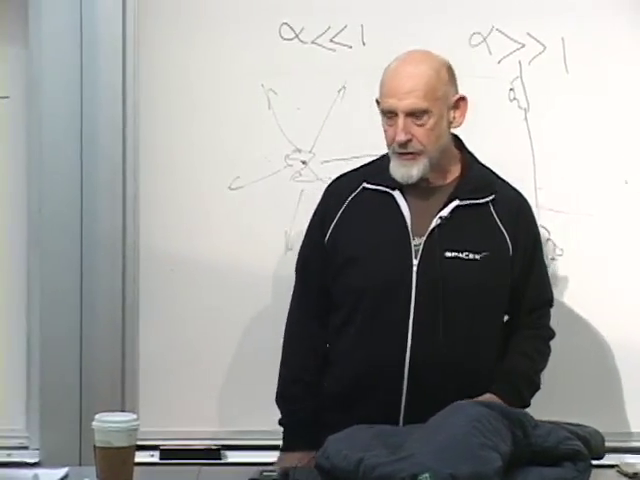
\includegraphics[width=0.72\textwidth]{lecture_01_figure_02.png}
\lectureframe{00:38:22.500}

\vspace{1em}

\begin{tikzpicture}[scale=0.95]
\draw (-5.3,-2.4) rectangle (-1.0,2.1);
\draw (0.3,-2.4) rectangle (4.6,2.1);

\node at (-3.15,2.55) {$\alpha \ll 1$};
\node at (2.45,2.55) {$\alpha \gg 1$};

\draw[line width=0.9pt] (-3.15,-0.15) circle (0.22);
\draw[->,line width=0.8pt] (-3.15,0.07) -- (-3.15,1.35);
\draw[->,line width=0.8pt] (-2.98,-0.01) -- (-1.95,1.00);
\draw[->,line width=0.8pt] (-3.32,-0.01) -- (-4.35,1.00);
\draw[->,line width=0.8pt] (-2.95,-0.23) -- (-1.80,-0.95);
\draw[->,line width=0.8pt] (-3.35,-0.23) -- (-4.50,-0.95);

\draw[line width=1.0pt] (2.15,-1.8) .. controls (1.95,-0.6) and (1.95,0.8) .. (2.15,1.55);
\draw[line width=1.0pt] (2.75,-1.8) .. controls (2.95,-0.6) and (2.95,0.8) .. (2.75,1.55);
\draw[line width=0.8pt] (2.15,-0.85) -- (2.75,-0.85);
\draw[line width=0.8pt] (2.45,1.55) -- (2.45,1.95);
\end{tikzpicture}
\caption{So sánh QED yếu--mạnh trong phần thảo luận về năng lượng tương tác. Hình vẽ tách riêng hai chế độ mà Susskind minh họa: một đám mây ghép yếu thưa loãng và một đám mây ghép mạnh tăng sinh.}
\end{figure}

Lý do hình này được đặt ở đây, dù phép so sánh yếu--mạnh đã được đưa ra trước đó, là vì trong bài giảng Susskind vẽ lại sự tương phản ấy ở thời điểm muộn hơn này do câu hỏi dẫn dắt, khi đang thảo luận về năng lượng tương tác và cấu trúc tăng sinh.

\section{Các lý thuyết brane chẵn và chiều không gian phụ xuất hiện}

Cho đến thời điểm này, bài giảng đã dựng nên một câu chuyện rất thuyết phục về sự hoán đổi: fermion so với boson, electron so với monopole, F-string so với D-string. Bước tiếp theo còn gây ngạc nhiên hơn. Susskind chuyển sang một phiên bản khác của lý thuyết dây, một phiên bản có các D-brane số chiều chẵn thay vì số chiều lẻ. Sự phân biệt này quan trọng vì trong lý thuyết đó không có D-string để hoán đổi với F-string. Ở đó có các D0-brane, D2-brane, D4-brane, v.v.

Vì thế, giới hạn ghép mạnh không thể đơn giản chỉ là việc đổi nhãn từ dây này sang dây khác. Theo bài giảng, có điều gì đó còn lạ hơn xảy ra: một chiều không gian phụ trở nên hiển lộ. Susskind cố ý phát biểu điều này trước hết dưới dạng kịch tính nhất --- ``một chiều mới xuất hiện'' --- rồi lập tức chuyển nó thành phát biểu cẩn trọng hơn: một chiều compact rất nhỏ nở ra cho đến khi không thể tiếp tục bỏ qua nữa.

Việc kiểm đếm này chính là một phần của ý chính, nên ông dừng lại ở đó:
\begin{equation}
\begin{aligned}
10\text{-dimensional string theory} &= 9\text{ space}+1\text{ time},\\
11\text{-dimensional theory} &= 10\text{ space}+1\text{ time}.
\end{aligned}
\end{equation}
Theo bài giảng, giới hạn ghép mạnh của lý thuyết brane chẵn về mặt hiệu dụng là mười một chiều.

\editorialnote{Lý thuyết brane chẵn là lý thuyết dây loại IIA, và sự hoàn chỉnh của nó trong miền liên kết mạnh là lý thuyết M. Trong các đơn vị chuẩn, bán kính của đường tròn xuất hiện và độ dài Planck mười một chiều tỉ lệ như \(R_{11}=g_s\ell_s\) và \(\ell_{11}=g_s^{1/3}\ell_s\). Những tên gọi và công thức này làm tường minh bảng đối chiếu hiện đại đứng sau cách trình bày hình học của bài giảng.}

\subsection{Bánh sandwich bơ đậu phộng}

Để hình dung chiều compact, Susskind dùng mô hình ``bánh sandwich bơ đậu phộng'': hai lát bánh mì mỏng vô hạn, với không gian thực ở giữa chúng. Quy tắc đặc biệt là đi ra ở một phía thì quay trở lại ở phía kia. Trong một ký hiệu thông thường mà bài giảng mô tả bằng hình ảnh hơn là bằng hình thức, ta có thể viết
\begin{equation}
y \sim y + 2\pi R.
\end{equation}
Nếu \(R\) rất nhỏ, những người quan sát sống trong chiếc sandwich đó sẽ mô tả thế giới của mình một cách hiệu dụng như có số chiều thấp hơn. Khi đó, cập nhật then chốt ở liên kết mạnh là
\begin{equation}
g\uparrow
\qquad \Longrightarrow \qquad
R_{\mathrm{compact}}\uparrow.
\end{equation}
Đó là điều Susskind muốn nói khi ông bảo rằng một chiều không gian mới xuất hiện: không phải không gian được tạo ra từ hư không, mà là một chiều compact vốn trước đây rất nhỏ nay nở ra và trở nên nhìn thấy được trong lý thuyết hiệu dụng.

\begin{figure}[htbp]
\centering
\resizebox{\linewidth}{!}{%
\begin{tikzpicture}[scale=0.95]
\draw[line width=0.9pt] (-5,1.7) -- (5,1.7);
\draw[line width=0.9pt] (-5,-1.7) -- (5,-1.7);

\node[left] at (-5,1.7) {ceiling};
\node[left] at (-5,-1.7) {floor};

\draw[->,line width=0.8pt] (5.2,1.45) -- (5.2,-1.45);
\draw[->,line width=0.8pt] (5.5,-1.45) -- (5.5,1.45);
\node[right] at (5.55,0) {periodic};

\draw[line width=1.0pt] (-2.6,0.45) -- (2.2,0.45);
\draw[line width=1.0pt] (-2.6,-0.05) -- (2.2,-0.05);
\draw[line width=1.0pt] (-2.6,0.45) -- (-2.6,-0.05);
\draw[line width=1.0pt] (2.2,0.45) -- (2.2,-0.05);
\node at (-0.2,0.9) {floating D2-brane};

\draw[line width=1.0pt] (3.15,-1.7) -- (3.8,-1.7);
\draw[line width=1.0pt] (3.15,1.7) -- (3.8,1.7);
\draw[line width=1.0pt] (3.15,-1.7) -- (3.15,1.7);
\draw[line width=1.0pt] (3.8,-1.7) -- (3.8,1.7);
\node[right] at (3.95,0) {D2 ribbon};

\fill (-3.8,0) circle (0.07);
\node[below] at (-3.8,-0.05) {D0};
\end{tikzpicture}
}%
\caption{Phép compact hóa kiểu sandwich. Biên trên và biên dưới được đồng nhất tuần hoàn; một D2-brane lơ lửng giữa chúng như một tấm thảm, còn một brane cùng loại khác kéo dài từ sàn lên trần và trông giống một dây khi chiều compact nhỏ.}
\end{figure}

\subsection{D0-brane và D2-brane sẽ ra sao?}

Bài giảng lúc này hỏi điều gì xảy ra với các D0-brane và các dây. Câu trả lời là bất đối xứng. Khi \(g\) trở nên lớn, các D0-brane ngày càng nhẹ đi; trong cách diễn giải cao chiều hơn, chúng gia nhập tháp các hạt mang xung lượng theo phương mới trở nên hiển hiện. Vì vậy, một đối tượng nặng nề, phức tạp trong mô tả liên kết yếu trở thành một kích thích nhẹ, thông thường trong mô tả liên kết mạnh.

Hệ thức khối lượng cho thấy sự đồng nhất sau đây:
\begin{equation}
M_{D0}(n)=\frac{n}{g_s\ell_s}
=\frac{n}{R_{11}}
=M_{\mathrm{KK}}(n).
\end{equation}
\editorialnote{Susskind gọi các D0-brane là ``các graviton'' của lý thuyết mười một chiều. Chính xác hơn, các trạng thái liên kết của chúng là các mode xung lượng Kaluza--Klein của bội siêu hấp dẫn mười một chiều, mà phần không khối lượng của nó chứa graviton. Sự phân biệt này giữ nguyên sự đồng nhất vật lý của bài giảng đồng thời tránh cách nói quá theo nghĩa đen như thể đó là một hạt đơn lẻ.}

Các D2-brane giải thích số phận của các dây. Có hai cấu hình được nhấn mạnh trong bài giảng:
\begin{enumerate}
\item một D2-brane lơ lửng giữa sàn và trần như một tấm thảm trong lớp bơ đậu phộng;
\item một D2-brane kéo dài từ sàn lên trần như một dải ruy băng, mở rộng theo phương nhìn thấy được.
\end{enumerate}
Khi chiếc sandwich mỏng, dải đó trông, về mặt hiệu dụng, như một đối tượng một chiều. Đó là đối tượng mà các quan sát viên năng lượng thấp gọi là một dây. Khi chiều compact mở ra, chính đối tượng ấy trở nên rõ ràng là giống màng. Vì giờ đây nó chứa nhiều vật chất hơn theo phương thẳng đứng, nó trở nên nặng và không còn giống dây nữa.

\paragraph{Lôgic của sự chuyển tiếp.}
\begin{enumerate}
\item Hãy bắt đầu với một chiều compact rất mảnh, để dải từ sàn tới trần ứng xử hiệu dụng như một sợi dây.
\item Tăng \(g\) lên, và chiều compact nở ra.
\item Các D0-brane trở nên nhẹ và được diễn giải lại như các trạng thái xung lượng Kaluza--Klein trong lý thuyết số chiều cao hơn.
\item Dải D2 giống dây trở thành một màng kéo dài thấy rõ và trở nên nặng.
\end{enumerate}
Đây là điểm bản lề của bài giảng khi chuyển từ đối ngẫu sang hình học xuất hiện. Liên kết mạnh không chỉ đơn thuần hoán đổi vật thể này lấy vật thể khác; nó thay đổi hình học nào mới là mô tả hữu hiệu.

Susskind dừng lại ở việc điều này nghe kỳ lạ đến mức nào. Mạng lưới các sự đồng nhất hóa được đề xuất đòi hỏi những quan hệ nhất quán toán học khó khăn, một số trong đó ban đầu xuất hiện trước các nhà vật lý như những phỏng đoán và về sau được các nhà toán học xác lập. Điều ông khẳng định không phải là mọi chân không dây thực tế đều đã được hiểu, mà là chính mạng lưới đối ngẫu ấy đã đứng vững qua những kiểm tra nghiêm ngặt khác thường.

Nếu hằng số liên kết biến thiên từ nơi này sang nơi khác trong thiết lập lý tưởng hóa này, thì mô tả hình học hữu hiệu cũng có thể biến thiên theo nó. Một vùng có thể trông gần như mười chiều, với các dây nhẹ và các D0-brane nặng; một vùng khác có thể mở ra thành mô tả mười một chiều, với các màng quấn nặng và các mode xung lượng Kaluza--Klein nhẹ. Sự thay đổi cục bộ của ngôn ngữ mô tả là một phần của cùng một mạng lưới đối ngẫu.

Bản ghi chép thoáng chốc chép tên của các quan hệ này thành ``các bất đẳng thức.'' Trong ngữ cảnh này, từ được nhắm tới là \emph{các đối ngẫu}: những quan hệ giữa các đầu đối nghịch của không gian tham số. Sự hiệu đính này quan trọng vì kết luận của bài giảng chính xác là không hề biết một danh sách duy nhất các thành phần cơ bản. Dây, brane, hạt và hình học nhiều chiều có thể biến đổi lẫn vào nhau; hoặc không thành viên nào của mạng lưới là tuyệt đối cơ bản, hoặc một sự tổ chức sâu hơn nào đó vẫn còn chưa biết.

\section{Các D3-brane, các màng quấn, và bức tranh hình học về đối ngẫu}

Sau giờ nghỉ, Susskind mô tả tường minh chủ đề này như một ``mạng lưới khổng lồ'' gồm các lý thuyết và ý tưởng liên kết với nhau. Các ví dụ tiếp theo không phải là những hiệu ứng cô lập mới; chúng là những cây cầu nối các ví dụ trước lại với nhau.

\subsection{Thể tích thế giới của một D3-brane}

Cây cầu đầu tiên sử dụng một D3-brane. Một D3-brane có ba chiều không gian, và một quan sát viên bị giới hạn trên nó có thể dễ dàng ngỡ đó là không gian thông thường. Brane có thể uốn cong và dao động, còn các dây kết thúc trên nó có thể nối lại, tách ra và tán xạ. Đối với một quan sát viên chỉ thấy các chiều dọc theo brane, mỗi đầu mút trông như một hạt và các tương tác giữa những đầu mút trông như một lý thuyết trường lượng tử thông thường.

\begin{figure}[htbp]
\centering
\resizebox{\linewidth}{!}{%
\begin{tikzpicture}[scale=1.0]
\draw[fill=gray!15] (-4,-0.35) rectangle (4,0.35);
\node at (0,-0.75) {D3-brane};

\draw[line width=0.9pt] (-1.5,2.1) -- (-1.5,0.35);
\fill (-1.5,0.35) circle (0.07);
\node[left] at (-1.72,1.25) {F-string};
\node[below left] at (-1.5,0.32) {electric charge};

\draw[line width=1.5pt] (1.7,2.1) -- (1.7,0.35);
\fill (1.7,0.35) circle (0.09);
\node[right] at (1.95,1.25) {D-string};
\node[below right] at (1.7,0.32) {magnetic monopole};
\end{tikzpicture}
}%
\caption{Diễn giải trên thể tích thế giới của D3-brane. Đầu mút của một F-string xuất hiện như một điện tích; đầu mút của một D-string xuất hiện như một đơn cực từ.}
\end{figure}

Đây là một trong những sự đồng nhất hóa thỏa đáng nhất của bài giảng. Một F-string kết thúc trên D3-brane xuất hiện đối với quan sát viên trên thể tích thế giới như một điện tích. Một D-string kết thúc trên cùng brane ấy xuất hiện như một đơn cực từ. Nói cách khác, đối ngẫu giữa F-string và D-string trở thành, trên thể tích thế giới của D3-brane, đối ngẫu điện--từ của lý thuyết trường thông thường. Điều trước đây là một phép tương tự nay đã trở thành một từ điển tường minh.

\editorialnote{Đối với một chồng các D3-brane, mô tả thể tích thế giới ở năng lượng thấp là lý thuyết Yang--Mills siêu đối xứng \(\mathcal N=4\) trong bốn chiều. Đối ngẫu điện--từ của nó là sự hiện thực hóa trong lý thuyết trường của đối ngẫu S của Type IIB; một brane đơn cho giới hạn Abel được dùng để minh họa bằng hình trong bài giảng.}

\subsection{Hai chiều compact và sự quấn bất đối xứng}

Sau đó Susskind quay trở lại hình học số chiều cao hơn và compact hóa không chỉ một mà hai chiều nhỏ. Vì không thể vẽ mười một chiều lên bảng, ông nén bảy chiều lớn không dùng trong hình phác thành một chiều ngang nhìn thấy được, rồi vẽ tường minh hai chiều compact. Ông nhấn mạnh phải vẽ phép compact hóa một cách bất đối xứng, vì một chiều compact phải ngắn hơn chiều kia nếu các dây hiệu dụng phải có lực căng khác nhau.

\begin{figure}[htbp]
\centering
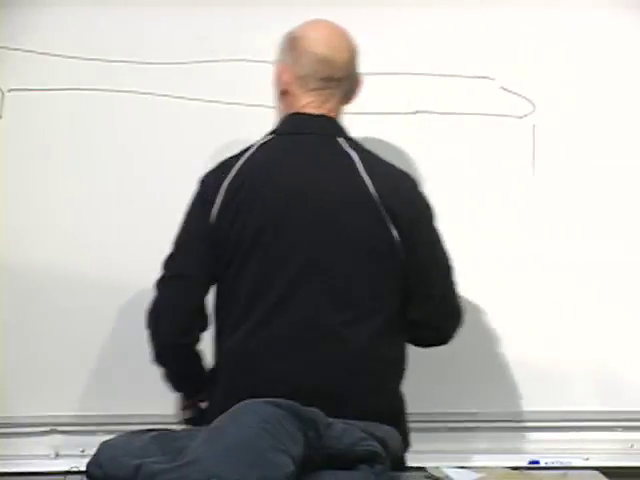
\includegraphics[width=0.78\textwidth]{lecture_01_figure_03.png}
\lectureframe{01:10:25.000}
\caption{Trạng thái hoàn chỉnh trên bảng của hai màng quấn. Chu trình compact ngắn và dài tạo ra các dải giống F-string và D-string được vẽ ở bên phải.}
\end{figure}

Một màng có thể quấn quanh một trong hai chiều compact và trông như một sợi dây khi nhìn từ các chiều không compact. Nếu \(R_1\) và \(R_2\) là hai bán kính vòng tròn, thì các lực căng hiệu dụng tương ứng của nó là
\begin{equation}
\begin{aligned}
T_{(1)}&=2\pi R_1 T_{\mathrm{M2}},\\
T_{(2)}&=2\pi R_2 T_{\mathrm{M2}},\\
\frac{T_{(1)}}{T_{(2)}}&=\frac{R_1}{R_2}.
\end{aligned}
\end{equation}
Do đó các kích thước vòng tròn không bằng nhau tạo ra các lực căng dây không bằng nhau. Nếu đồng nhất cách quấn theo chu trình ngắn hơn với F-string nhẹ và theo chu trình dài hơn với D-string nặng, ta có thể viết một cách sơ đồ
\begin{equation}
g_s\sim \frac{R_{\mathrm{short}}}{R_{\mathrm{long}}},
\qquad
\frac{T_{\mathrm{D1}}}{T_{\mathrm{F1}}}\sim \frac{1}{g_s}.
\end{equation}

\begin{classroomqa}
\audiencequestion{Liệu hằng số liên kết trong bức tranh này có thể được hiểu như tỉ số của hai chiều compact không? \lecturetimestamp{01:10:13}}
\lecturerresponse{Có. Tham số yếu--mạnh được hình học hóa thành một tỉ lệ cạnh. Làm cho một chiều ngắn đi tạo ra liên kết nhỏ; đổi chỗ hai chiều sẽ hoán đổi dây nhẹ và dây nặng.}
\end{classroomqa}

\editorialnote{Bài giảng tạm thời gọi tỉ số này là \(\alpha\), dùng lại ký hiệu trước đó đã dùng cho hằng số cấu trúc tinh tế của QED. Ở đây chúng tôi viết \(g_s\) để giữ cho hai nghĩa tách biệt nhau. Trong cấu trúc M-theory đầy đủ, hằng số liên kết Type IIB được mã hóa trong cấu trúc phức của xuyến compact hai chiều; tử số chính xác phụ thuộc vào cách các chu trình của nó được gán nhãn.}

Bức tranh màng quấn có thể được tóm tắt mà không cần đến phép méo phối cảnh của hình vẽ trên bảng:

\begin{figure}[htbp]
\centering
\begin{tikzpicture}[scale=1.0]
\draw[line width=0.9pt] (0,0) rectangle (5.2,2.2);
\node[below] at (2.6,-0.2) {\(R_1\)};
\node[right] at (5.4,1.1) {\(R_2\)};

\draw[->,line width=0.7pt] (5.45,1.9) -- (5.45,0.3);
\draw[->,line width=0.7pt] (5.7,0.3) -- (5.7,1.9);
\draw[->,line width=0.7pt] (0.4,-0.35) -- (4.8,-0.35);
\draw[->,line width=0.7pt] (4.8,-0.6) -- (0.4,-0.6);

\draw[line width=1.0pt] (1.1,0) -- (1.6,0) -- (1.6,2.2) -- (1.1,2.2) -- cycle;
\node at (1.35,2.55) {light};

\draw[line width=1.0pt] (0,1.45) -- (5.2,1.45);
\draw[line width=1.0pt] (0,1.00) -- (5.2,1.00);
\node at (4.55,1.95) {heavy};

\node at (1.35,-0.95) {F-string};
\node at (4.55,0.55) {D-string};
\end{tikzpicture}
\caption{Cả hai cấu hình màng quấn đều trông giống dây khi nhìn từ các chiều không compact, nhưng các thang compact không bằng nhau khiến một dây hiệu dụng nhẹ hơn dây kia.}
\end{figure}

Đây là phiên bản hình học của câu chuyện đối ngẫu trước đó. Thu ngắn một chiều trong khi kéo dài chiều kia làm một vật thể quấn nặng hơn và vật thể còn lại nhẹ hơn, vì thế vai trò của F-string và D-string có thể hoán đổi cho nhau.

\begin{classroomqa}
\audiencequestion{Nếu các chiều compact là tuần hoàn, các vật thể quấn có rộng vô hạn không? \lecturetimestamp{01:10:41}}
\lecturerresponse{Không. Một đường tròn compact có chu vi hữu hạn mặc dù ta có thể đi quanh nó lặp đi lặp lại mà không chạm tới mép. Phần trên và phần dưới của hình vẽ đã cắt mở biểu diễn cùng một điểm, cũng như hai đầu mút của một đoạn có thể biểu diễn một điểm của đường tròn.}
\end{classroomqa}

\begin{figure}[htbp]
\centering
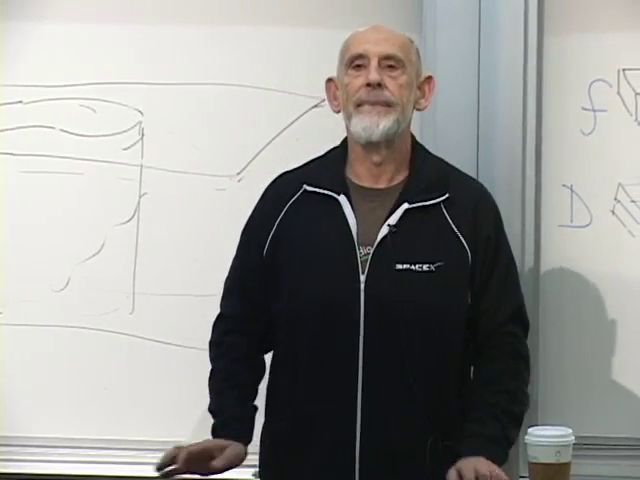
\includegraphics[width=0.78\textwidth]{lecture_01_figure_04.png}
\lectureframe{01:12:25.000}

\vspace{1em}

\begin{tikzpicture}[scale=0.95]
\draw[line width=0.9pt,->] (-3.7,0) arc[start angle=180,end angle=535,radius=0.95];
\node at (-2.75,0) {compact circle};
\draw[line width=0.9pt] (0.0,0) -- (4.8,0);
\fill (0.0,0) circle (0.06);
\fill (4.8,0) circle (0.06);
\draw[<->] (0.0,-0.45) -- (4.8,-0.45);
\node at (2.4,-0.75) {cut-open interval of length \(2\pi R\)};
\node[above] at (0.0,0.1) {same point};
\node[above] at (4.8,0.1) {same point};
\end{tikzpicture}
\caption{Một đường tròn compact và biểu diễn đã cắt mở của nó trên bảng. Đi qua một đầu mút sẽ trở lại ở đầu kia; còn đi quanh đường tròn đồng thời di chuyển theo một chiều không compact thì sẽ vạch ra một đường xoắn ốc.}
\end{figure}

\begin{classroomqa}
\audiencequestion{Tại sao đường đi theo chiều compact là một đường tròn chứ không phải một đường xoắn ốc? \lecturetimestamp{01:12:23}}
\lecturerresponse{Ở mỗi điểm cố định theo chiều không compact, chiều compact là một đường tròn. Chỉ khi ta tiến theo chiều không compact đồng thời quấn quanh đường tròn thì đường xoắn ốc mới xuất hiện. Đoạn trên bảng đơn giản chỉ là một đường tròn bị cắt mở, với hai đầu mút của nó được đồng nhất.}
\end{classroomqa}

\begin{classroomqa}
\audiencequestion{Liệu chính hình học này có giải thích được vì sao một D-brane có thể trông như một tập hợp các F-string khi bị thăm dò ở khoảng cách nhỏ không? \lecturetimestamp{01:12:49}}
\lecturerresponse{Mối liên hệ là có, nhưng nó không hiển nhiên trong bức tranh sơ cấp này; để thấy được điều đó cần thêm công cụ hình học. Hình vẽ nhằm tổ chức đối ngẫu, chứ không suy ra mọi mô tả thành phần vi mô.}
\end{classroomqa}

\begin{classroomqa}
\audiencequestion{Liệu chiều compact dài và ngắn có thể hoán đổi khi ta di chuyển trong không gian, hoặc khi thời gian tiến triển không? \lecturetimestamp{01:13:35}}
\lecturerresponse{Cả hai đều có thể trong mô hình lý tưởng hóa. Ép một chu trình lại trong khi làm nở chu trình kia sẽ hoán đổi dây quấn nào là nhẹ. Đây là một lý do nữa khiến ``dây cơ bản'' chỉ là một cái tên: mô tả được ưu tiên có thể thay đổi từ vùng này sang vùng khác hoặc theo thời gian.}
\end{classroomqa}

\section{Sự lý tưởng hóa, các điểm đối xứng đặc biệt và cảnh quan}

Phần cuối của bài giảng lùi ra khỏi những ví dụ đối ngẫu thanh nhã và hỏi xem chúng cho ta biết gì, và không cho ta biết gì, về thế giới thực.

Trước hết, Susskind cảnh báo rằng các đối ngẫu được kiểm soát chính xác là những đặc trưng của các lý thuyết siêu đối xứng đã được lý tưởng hóa cao độ, trong đó boson và fermion có khối lượng khớp nhau một cách chính xác. Phép tương tự của ông là các quỹ đạo tròn trong cơ học Newton: người ta nghiên cứu chúng trước tiên vì chúng đối xứng và dễ xử lý về toán học, chứ không phải vì chuyển động hành tinh thực tế được mô tả trọn vẹn bởi những đường tròn hoàn hảo. Hoàn toàn tương tự, các lý thuyết dây siêu đối xứng dễ phân tích hơn vì chúng đối xứng hơn mức mà tự nhiên dường như có.

Tuy vậy, sự lý tưởng hóa vẫn đem lại thông tin. Một quỹ đạo tròn hoàn hảo không phải là một hệ hành tinh thực tế, nhưng nó phô bày những đặc điểm còn tồn tại trong các quỹ đạo kém đối xứng hơn. Tương tự, các ví dụ siêu đối xứng cho thấy những cách nhất quán để cơ học lượng tử, hấp dẫn và cấu trúc vi mô có thể khớp với nhau. Cách phát biểu cố ý sắc gọn của Susskind là các lý thuyết dây có thể xử lý được không, theo nghĩa đen, phải là lý thuyết của thế giới chúng ta; giá trị của chúng nằm ở chỗ chúng bộc lộ những hiện tượng có khả năng xuất hiện trở lại trong những bối cảnh kém đối xứng hơn và khó xử lý hơn.

\subsection{Một bộ lắp ghép với nhiều kết quả}

D-brane chỉ là một phần của bộ lắp ghép sẵn có. Bài giảng cũng nhắc tới các thông lượng, orbifold và orientifold. Trước hết ta chọn một hình học compact, rồi chọn những brane và thông lượng nào chiếm các chu trình của nó. Ngay cả cấu hình sandwich đơn giản ấy cũng làm thay đổi vật lý số chiều thấp hơn khi ta chèn vào một D2-brane lơ lửng, hai cái, hoặc ba cái. Việc thêm hoặc bớt những thành phần như thế làm thay đổi các hạt, các tương tác và các tham số hiệu dụng.

Giả sử, theo phép đếm sơ đồ của bài giảng, một không gian compact sáu chiều có xấp xỉ \(500\) chu trình và mỗi chu trình chấp nhận cỡ \(10\) lựa chọn về brane quấn, thông lượng hoặc các cấu trúc liên quan. Khi đó số cách xây dựng tăng như
\begin{equation}
N_{\mathrm{vacua}} \sim 10^{500}.
\end{equation}
Lôgic đếm của bài giảng là sơ đẳng:
\begin{equation}
10 \times 10 \times \cdots \times 10 = 10^{500}
\end{equation}
với \(500\) thừa số. Phép tương tự với DNA nêu cùng ý đó trong một ngữ cảnh quen thuộc hơn:
\begin{equation}
N_{\mathrm{DNA}}(500)=4^{500}.
\end{equation}
Trong lúc so sánh với DNA, một người trong cử tọa kiểm tra rằng dọc theo một sợi có bốn khả năng: A, C, G và T. Sự đính chính ấy củng cố chứ không thay đổi lập luận. Một danh sách ngắn các lựa chọn cục bộ, được lặp lại nhiều lần, tạo ra một số lượng khổng lồ các cách sắp xếp toàn cục. Số mũ chính xác không phải là điều cốt yếu, và Susskind gọi \(10^{500}\) là một sự đánh giá thấp đã cũ; điểm mấu chốt là sự bùng nổ tổ hợp.

Điều này đem lại sự đảo ngược cuối cùng của kỳ vọng quy giản luận mở đầu. Vật lý hạt phức tạp không nhất thiết phải phát sinh từ các quy tắc vi mô phức tạp. Nó có thể phát sinh vì chân không của chúng ta là một cách sắp đặt phức tạp của nhiều thành phần đơn giản, cũng như một sinh vật phức tạp có thể được mã hóa bởi một chuỗi được xây từ bốn bazơ.

\begin{classroomqa}
\audiencequestion{Sau khi các mô tả tương đương có liên hệ với nhau bởi đối ngẫu đã được đồng nhất, liệu thông tin đầy đủ có chỉ chọn ra một hoặc vài chân không khả dĩ trong số này làm mô tả về thế giới của chúng ta không? \lecturetimestamp{01:26:11}}
\lecturerresponse{Có lẽ nó sẽ chọn ra một tập bị hạn chế, nhưng nhiều chân không phân biệt có thể trông cực kỳ giống nhau ở các năng lượng có thể tiếp cận. Con số cảnh quan được nêu ra được hiểu là vẫn còn lớn ngay cả sau khi các mô tả đối ngẫu đã được đồng nhất, và những chi tiết năng lượng cao không liên quan có thể hoạt động như ``DNA rác.''}
\end{classroomqa}

\subsection{Các điểm đối xứng và độ phức tạp điển hình}

Trong landscape có những điểm đối xứng đặc biệt. Trong bức tranh hình học, một cấu hình có tỷ lệ bằng nhau,
\begin{equation}
R_1=R_2,
\end{equation}
làm cho hai mô tả bằng dây quấn đơn giản ngang nhau. Trong phép tương tự điện--từ, điều này được biểu diễn một cách sơ đồ bởi
\begin{equation}
m_{\mathrm{monopole}}=m_e.
\end{equation}

\begin{figure}[htbp]
\centering
\begin{tikzpicture}[scale=0.95]
\draw[line width=0.9pt] (-4.5,-1.0) rectangle (-2.5,1.0);
\draw[<->] (-4.5,-1.35) -- (-2.5,-1.35);
\draw[<->] (-2.15,-1.0) -- (-2.15,1.0);
\node at (-3.5,1.45) {symmetric point};
\node at (-3.5,-1.75) {$R_1=R_2$};

\draw[line width=0.9pt] (0.0,-0.55) rectangle (4.8,0.55);
\draw[<->] (0.0,-0.9) -- (4.8,-0.9);
\draw[<->] (5.15,-0.55) -- (5.15,0.55);
\node at (2.4,1.45) {lopsided point};
\node at (2.4,-1.3) {$R_1\ne R_2$};
\end{tikzpicture}
\caption{Phép compact hóa có tỷ lệ bằng nhau đặt hai dây quấn vào vị thế đối xứng; phép compact hóa bất cân xứng làm cho một mô tả nhẹ hơn rất nhiều so với mô tả kia.}
\end{figure}

\begin{classroomqa}
\audiencequestion{Có những chân không nào trong landscape mà ở đó cách xây dựng trở nên đơn giản hơn nhiều vì các mô tả bằng F-string và D-string trùng nhau không? \lecturetimestamp{01:27:21}}
\lecturerresponse{Có, có những điểm đối xứng đặc biệt. Thế giới của chúng ta dường như không ở một điểm như vậy: hạt điện quen thuộc và một đơn cực từ không có khối lượng bằng nhau. Vì sao tự nhiên lại ở một điểm bất cân xứng như vậy thì chưa rõ.}
\end{classroomqa}

\editorialnote{Việc electron--đơn cực có khối lượng bằng nhau là một đặc trưng có tính sơ đồ của một mô hình tự đối ngẫu được bảo vệ thích hợp, chứ không phải dự đoán của QED thông thường không siêu đối xứng. Nó diễn đạt ý tưởng về điểm đối xứng của bài giảng, chứ không phải một khẳng định về electron quan sát được.}

Susskind sau đó nhắc lại một phép tương tự từ lý thuyết truyền thông. Các mã ngẫu nhiên có thể tốt một cách phi thường, trong khi các mã dễ mô tả và giải mã nhất lại có cấu trúc toán học bổ sung và trong lịch sử thường cho hiệu năng kém hơn. Về sau lý thuyết mã hóa đã tìm ra những cách xây dựng có cấu trúc rất hiệu quả, nhưng phép tương tự vẫn còn nguyên: bất cứ thứ gì có thể được gọi tên hoặc mô tả một cách gọn ghẽ đều nằm ở một góc rất đặc biệt, có độ phức tạp thấp, của toàn bộ không gian các khả thể. Tương tự như vậy, những chân không của lý thuyết dây dễ tính toán nhất có thể đơn giản một cách không điển hình.

Vì thế, những câu hỏi thích hợp có thể thay đổi. Thay vì đòi hỏi phép compact hóa chính xác đến từng chi tiết vi mô, ta có thể hỏi những đặc trưng nào là chung hoặc điển hình trong một tập hợp rộng. Susskind trình bày điều này như một vấn đề nghiên cứu, không phải một kết luận đã ngã ngũ, và bác bỏ các lập luận mang tính ý thức hệ thay cho tính toán.

\subsection{Các câu hỏi vũ trụ học}

\begin{classroomqa}
\audiencequestion{Một chiều compact có chu vi cực lớn có khác biệt được về mặt quan sát so với một chiều vô hạn không, và chúng ta có biết ba chiều không gian lớn của mình là vô hạn không? \lecturetimestamp{01:30:03}}
\lecturerresponse{Chúng ta không biết rằng chúng là vô hạn. Một 3-cầu kín có thể giãn nở mà vẫn compact. Các phép đo độ gần phẳng chỉ cho một cận dưới đối với bán kính độ cong, cũng như việc khảo sát một cánh đồng gần như phẳng có thể đặt cận dưới cho kích thước Trái Đất mà không chứng minh rằng bề mặt của nó là vô hạn. Chỉ khi phát hiện được độ cong hoặc một phép đồng nhất toàn cục thì mới xác định được thang độ hữu hạn ấy.}
\end{classroomqa}

\begin{classroomqa}
\audiencequestion{Nếu độ ghép có thể biến thiên theo không gian trong mô hình lý tưởng hóa, thì trong thế giới thực một sự biến thiên như vậy có thể xảy ra như thế nào? \lecturetimestamp{01:32:43}}
\lecturerresponse{Không phải theo kiểu biến thiên trơn, không bị hạn chế, đã dùng trong ví dụ đối xứng. Khả năng thực tế sẽ được bàn sau là sự biến thiên thông qua các chuyển tiếp rời rạc giữa những vùng có các quy luật hiệu dụng khác nhau. Việc những bước nhảy như thế có xảy ra hay không là một câu hỏi vũ trụ học.}
\end{classroomqa}

\editorialnote{Cần đọc câu trả lời này như phần báo trước của bài giảng về các chân không thông lượng và các chuyển tiếp miền, chứ không phải như một định lý tổng quát cấm mọi trường vô hướng biến thiên trơn. Các quan sát ràng buộc rất chặt các biến thiên của những độ ghép không thứ nguyên, còn các cơ chế ổn định hóa quyết định liệu trong một mô hình cho trước vẫn còn các moduli liên tục hay không.}

Bản ghi không lưu lại câu hỏi cuối cùng của cử tọa. Phần trả lời còn sót lại nói rằng hiện tượng được nêu ra có thể xảy ra đối với một số loại lỗ đen nhưng không xảy ra ở chân trời của một lỗ đen Schwarzschild thông thường, mà chân trời của nó xét cục bộ là một nơi bình thường đối với một quan sát viên rơi tự do. Vì không thể khôi phục câu hỏi ấy một cách đáng tin cậy, nên không quy cho cuộc trao đổi này một khẳng định cụ thể nào hơn.

\section{Từ những viên gạch đến một mạng lưới các mô tả}

Hy vọng rằng các tầng sâu hơn của vật lý tất phải đơn giản hơn đã tỏ ra mong manh. Trong boson hóa \(1+1\) chiều, cùng một lý thuyết có thể được tổ chức hoặc theo fermion hoặc theo boson, với fermion xuất hiện trở lại dưới dạng một kink. Trong điện động lực học lượng tử, ghép yếu và ghép mạnh hoán đổi vai trò mô tả của electron và đơn cực từ. Trong lý thuyết dây, F-string và D-string lặp lại cùng một khuôn mẫu ấy, còn trong lý thuyết các brane chẵn, ghép mạnh còn đi xa hơn nữa: một chiều compact nở ra, các D0-brane trở thành các trạng thái xung lượng Kaluza--Klein, và các dây hiệu dụng được diễn giải lại như các màng quấn trong một hình học số chiều cao hơn. Vì vậy, lý thuyết trường lượng tử hiện đại và lý thuyết dây không cung cấp một câu trả lời duy nhất và dứt khoát cho câu hỏi ``đâu là những viên gạch và đâu là những ngôi nhà?'' Chúng cung cấp một mạng lưới các mô tả, mỗi mô tả hữu hiệu trong miền riêng của nó, cùng với một landscape khổng lồ của các cách xây dựng khả dĩ mà kết quả điển hình là sự phức tạp chứ không phải sự đơn giản.

\chapter{Hình học, thông tin và định luật diện tích của lỗ đen}

\lectureoverview{Điểm đến đã được báo trước là vũ trụ học, nhưng con đường ngắn nhất tới đó lại bắt đầu bằng việc quay về thuyết tương đối hẹp. Metric cho ta biết hình học của không-thời gian, còn điều kiện thời gian riêng bằng không cho ta biết ánh sáng truyền như thế nào. Chúng ta sẽ mang quy tắc duy nhất ấy vào hình học Schwarzschild, phân biệt chân trời với kỳ dị, rồi hỏi thông tin sẽ ra sao khi một lỗ đen bức xạ dần mất đi. Câu trả lời bắt đầu từ entropy thông thường và kết thúc ở lập luận một bit của Bekenstein: lỗ đen lưu trữ thông tin theo đơn vị diện tích chân trời chứ không phải thể tích.}

Susskind tạm gác ngắn gọn bản tổng kết đã hứa về những thành công và thất bại của lý thuyết dây. Ông nói đã muộn, và nội dung thực chất hữu ích hơn một cuộc kiểm kê. Nội dung thực chất tối nay là phần hình học và nhiệt động lực học tối thiểu cần để phát biểu bài toán thông tin của lỗ đen.

\section{Một quy tắc duy nhất cho ánh sáng}

Thuyết tương đối hẹp xem không gian và thời gian là một đối tượng hình học duy nhất. Với các biến cố lân cận cách nhau bởi \(dt,dx,dy,dz\), Susskind dùng quy ước chủ yếu dấu trừ và viết
\begin{equation}
d\tau^2=dt^2-\frac{1}{c^2}\left(dx^2+dy^2+dz^2\right).
\end{equation}
Dấu trái ngược nhau của phần thời gian và phần không gian phân biệt hình học Minkowski với hình học Euclid bốn chiều. Hệ số \(1/c^2\) chỉ đơn thuần điều hòa đơn vị; bằng cách đo thời gian và khoảng cách theo những đơn vị tương thích, ta có thể đặt \(c=1\).

Với khoảng tách kiểu thời gian \(d\tau^2>0\), và \(d\tau\) là thời gian riêng được một chiếc đồng hồ đi theo quỹ đạo ấy ghi lại. Trái lại, các khoảng tách kiểu không gian có \(d\tau^2<0\). Trường hợp cần cho tối nay nằm đúng giữa hai loại đó. Một tia sáng đi theo quỹ đạo \emph{null},
\begin{equation}
d\tau^2=0.
\end{equation}
Trước hết giới hạn vào chuyển động dọc theo trục \(x\) thì được
\begin{align}
0&=dt^2-\frac{dx^2}{c^2},\\
c\,dt&=\pm dx,\\
\frac{dx}{dt}&=\pm c.
\end{align}
Các dấu mô tả các tia đi sang phải và sang trái. Giá trị số gán cho \(c\) thay đổi khi thay xentimét bằng mét hay kilômét; mệnh đề bất biến không phải là một con số mà là điều kiện null.

Thuyết tương đối rộng làm metric phức tạp hơn, chứ không phải quy tắc này. Với các tọa độ \(x^\mu\), \(\mu=0,1,2,3\),
\begin{equation}
ds^2=g_{\mu\nu}(x)\,dx^\mu dx^\nu,
\end{equation}
trong đó các chỉ số lặp được lấy tổng và các hệ số có thể thay đổi từ điểm này sang điểm khác. Để tìm các hướng truyền ánh sáng được phép cục bộ, hãy cho dạng toàn phương này bằng không.

\section{Tọa độ cầu và metric Schwarzschild}

Một lỗ đen không quay có đối xứng cầu, vì vậy tọa độ Cartesian che khuất cấu trúc hữu ích. Hãy để \(r\) đo khoảng cách xuyên tâm và \(\theta,\phi\) xác định một hướng trên mặt cầu đơn vị. Phần tử độ dài của nó là
\begin{equation}
d\Omega^2=d\theta^2+\sin^2\theta\,d\phi^2.
\end{equation}
Vì thế, trên một mặt cầu bán kính \(r\), các độ dời góc đóng góp \(r^2d\Omega^2\). Không-thời gian phẳng trong tọa độ cầu là
\begin{equation}
d\tau^2=dt^2-\left(dr^2+r^2d\Omega^2\right),
\qquad (c=1).
\end{equation}

Susskind không suy ra nghiệm lỗ đen từ các phương trình Einstein. Ông viết nó ra và yêu cầu chúng ta xem xét nó. Bảng viết làm rõ sự so sánh được nhắm tới.

\begin{figure}[htbp]
\centering
\includegraphics[width=0.86\textwidth]{lecture_02_figure_02.png}
\caption{Không-thời gian phẳng trong tọa độ cầu nằm phía trên biến dạng Schwarzschild. Hệ số lặp lại \(1-2GM/(c^2r)=1-R_s/r\) và phác thảo theo phương bán kính được thấy cùng nhau.}
\lectureframe{00:19:12.520}
\end{figure}

Đối với một lỗ đen khối lượng \(M\), định nghĩa bán kính Schwarzschild
\begin{equation}
R_s=\frac{2GM}{c^2}.
\end{equation}
Phần tử độ dài bên ngoài là
\begin{equation}
d\tau^2=\left(1-\frac{R_s}{r}\right)dt^2
-\frac{dr^2/c^2}{1-R_s/r}
-\frac{r^2}{c^2}d\Omega^2.
\label{eq:schwarzschild-explicit-c}
\end{equation}
Tương đương, sau khi đặt \(c=1\),
\begin{equation}
ds^2=\left(1-\frac{2GM}{r}\right)dt^2
-\frac{dr^2}{1-2GM/r}-r^2d\Omega^2.
\label{eq:schwarzschild}
\end{equation}
Ở rất xa, \(R_s/r\ll1\), và metric phẳng trong tọa độ cầu lại xuất hiện. Phép kiểm tra tiệm cận này quan trọng hơn việc học thuộc công thức, dù Susskind khuyên nên làm điều sau như vốn liếng cho các buổi tiệc cocktail.

\editorialnote{Bảng viết luân phiên giữa \(d\tau^2\) và \(ds^2\) và không hiển thị nhất quán mọi hệ số của \(c\). Phương trình~\eqref{eq:schwarzschild-explicit-c} tuân theo quy ước tọa độ thời gian của bài giảng, trong đó \(t\) có đơn vị thời gian. Dạng chuẩn với \(x^0=ct\) là tương đương về mặt đại số.}

\subsection{Chân trời không phải là kỳ dị}

Có hai bán kính trông đáng ngờ trong các tọa độ này. Tại \(r=R_s=2GM\) trong đơn vị tự nhiên, hệ số của \(dt^2\) triệt tiêu còn hệ số của \(dr^2\) phân kỳ. Tại \(r=0\), bản thân độ cong trở nên kỳ dị. Đây không phải là hai phiên bản của cùng một sự kiện:
\begin{equation}
\begin{aligned}
r=R_s &:\quad \text{horizon},\\
r=0 &:\quad \text{curvature singularity}.
\end{aligned}
\end{equation}

Các lực thủy triều cho ta sự phân biệt vật lý. Trường hấp dẫn biến thiên trên một vật thể có kích thước: chân có thể bị kéo mạnh hơn đầu, làm vật thể bị kéo dài ra trong khi các phương ngang bị ép lại. Tại chân trời, các lực thủy triều ấy là hữu hạn, và tại chân trời của một lỗ đen đủ lớn chúng có thể rất nhỏ. Không nhất thiết có điều gì thảm khốc cục bộ xảy ra ở đó. Ngược lại, tại \(r=0\), các lực thủy triều phân kỳ. Những hệ số đáng báo động tại \(r=R_s\) báo hiệu một khuyết tật của tọa độ Schwarzschild; kỳ dị tại \(r=0\) mới là vật lý.

\editorialnote{Tính hữu hạn của độ cong tại \(r=R_s\) có thể được kiểm tra từ vô hướng Kretschmann \(R_{\mu\nu\rho\sigma}R^{\mu\nu\rho\sigma}=48G^2M^2/(c^4r^6)\), đại lượng này hữu hạn ở chân trời và chỉ phân kỳ khi \(r\to0\). Bất biến này không được viết ra trong bài giảng, nhưng nó làm cho sự phân biệt bằng lực thủy triều ở trên trở nên chính xác.}

\section{Ánh sáng theo phương bán kính gần chân trời}

Giờ hãy quay lại quy tắc duy nhất ấy. Một tia theo phương bán kính giữ cố định vị trí góc của nó, nên \(d\Omega=0\), và tia sáng có \(ds^2=0\). Trong đơn vị \(c=1\), Phương trình~\eqref{eq:schwarzschild} cho
\begin{equation}
0=\left(1-\frac{2GM}{r}\right)dt^2
-\frac{dr^2}{1-2GM/r}.
\end{equation}
Nhân với \(1-2GM/r\) rồi lấy căn bậc hai cho hai nhánh,
\begin{align}
dr&=\pm\left(1-\frac{2GM}{r}\right)dt,\\
\frac{dr}{dt}&=\pm\left(1-\frac{2GM}{r}\right).
\label{eq:radial-null}
\end{align}
Dấu cộng là tia đi ra và dấu trừ là tia đi vào. Ở rất xa, các tốc độ tọa độ của chúng tiến tới \(\pm1\). Tại chân trời, cả hai đều thỏa \(\lvert dr/dt\rvert\to0\): theo thời gian tọa độ Schwarzschild, một tia đi ra dường như đứng yên ở đó, còn một tia đi vào cần thời gian tọa độ vô hạn để tới nơi.

\begin{figure}[htbp]
\centering
\includegraphics[width=0.82\textwidth]{lecture_02_figure_03.png}
\caption{Bản phác thảo bảng đen \(t\)-\(r\) đã hoàn chỉnh: các tia null theo phương bán kính trở nên gần như thẳng đứng khi tiến tới chân trời nét đứt.}
\lectureframe{00:30:25.000}
\end{figure}

\begin{figure}[htbp]
\centering
\begin{tikzpicture}[x=1.0cm,y=0.9cm]
\draw[->] (0,0) -- (6.6,0) node[right] {$r$};
\draw[->] (0,0) -- (0,6.2) node[above] {$t$};
\draw[dashed,thick] (2.0,0) -- (2.0,5.9) node[above] {$r=R_s$};
\draw[thick,->] (2.08,.4) .. controls (2.10,2.2) and (2.55,3.8) .. (5.8,5.7);
\draw[thick,->] (5.8,.5) .. controls (3.2,2.0) and (2.15,4.2) .. (2.03,5.7);
\node[align=center] at (4.7,4.4) {outgoing};
\node[align=center] at (4.5,1.2) {ingoing};
\end{tikzpicture}
\caption{Phiên bản theo thời gian tọa độ đã được làm gọn của bản phác thảo trên bảng. Sự chậm lại biểu kiến là một phát biểu về \(t\) trong tọa độ Schwarzschild, không phải về việc ánh sáng cục bộ không còn chuyển động với \(c\).}
\end{figure}

Bên trong chân trời, các nón ánh sáng tương lai nghiêng vào trong đến mức cả hai nhánh theo phương bán kính hướng về tương lai đều dẫn tới \(r\) giảm. Không tín hiệu nào phát sinh ở đó có thể thoát ra ngoài, và mọi đường nhân quả hướng về tương lai đều đi tới kỳ dị.

\begin{classroomqa}
\audiencequestion{Nếu tốc độ ánh sáng là bất biến, thì nói chính xác là gì khi bảo rằng ánh sáng chậm lại gần chân trời?\lecturetimestamp{00:31:44}}
\lecturerresponse{Đại lượng được hiển thị là \(dr/dt\) trong một hệ tọa độ cụ thể. Tốc độ dưới dạng giá trị số đã thay đổi khi mét được thay bằng xentimét; ở đây các chuẩn hiệu dụng theo phương bán kính và theo thời gian còn biến thiên theo vị trí. Mệnh đề phổ quát là mọi tia sáng đều đi theo một quỹ đạo null, \(ds^2=0\).}
\end{classroomqa}
\editorialnote{Một quan sát viên cục bộ rơi tự do đo ánh sáng trong chân không là \(c\); việc vận tốc theo tọa độ Schwarzschild triệt tiêu ở chân trời không phải là một đại lượng quan sát cục bộ.}

\begin{classroomqa}
\audiencequestion{Mệnh đề về tốc độ null ấy có còn đúng bất kể ánh sáng truyền qua môi trường vật chất nào hay không?\lecturetimestamp{00:33:24}}
\lecturerresponse{Không. Tư liệu hiện có không còn lưu phần giải thích dài hơn cho câu trả lời này.}
\end{classroomqa}
\editorialnote{Khẳng định về tốc độ null nói về sự lan truyền trong không-thời gian chân không. Tương tác với vật chất có thể khiến một gói sóng có tốc độ hiệu dụng nhỏ hơn; đó là tính chất của môi trường, không phải sự thay đổi của tốc độ nhân quả cục bộ \(c\).}

\begin{classroomqa}
\audiencequestion{Một tia sáng đi vào trông như thế nào trên cùng giản đồ \(t\)-\(r\)?\lecturetimestamp{00:33:32}}
\lecturerresponse{Đó là nhánh có hình dạng ngược lại: từ \(r\) lớn, nó uốn về phía chân trời và tiến tới đó một cách tiệm cận. Nó cần một lượng thời gian tọa độ \(t\) vô hạn để tới nơi.}
\end{classroomqa}
\editorialnote{Một quan sát viên rơi vào tới chân trời và đi qua nó trong thời gian riêng hữu hạn; chỉ có \(t\) Schwarzschild là phân kỳ.}

\section{Vì sao sự bay hơi tạo ra một vấn đề}

Chân trời còn đáng được nghiên cứu nhiều hơn nữa: nó hình thành ra sao, người quan sát rơi vào thấy gì, và liệu ở đó có điều gì bất thường về cục bộ hay không. Susskind hoãn các câu hỏi ấy lại và chuyển thẳng sang cơ học lượng tử. Từ bên ngoài nhìn vào, vật chất cùng toàn bộ thông tin phân biệt của nó bị nén ngày càng sát chân trời hơn và trở nên không thể tiếp cận. Chỉ riêng điều đó chưa nhất thiết hủy diệt thông tin; có thể nó chỉ đơn giản là che giấu thông tin.

Kết quả của Hawking làm vấn đề trở nên gay gắt. Một lỗ đen cổ điển đã ổn định trông như vật thể tẻ nhạt nhất có thể tưởng tượng: có đối xứng cầu, tối, và không thể gửi đi một thông điệp. Nhưng ``đen'' có hai nghĩa. Nó có thể có nghĩa là không phát ra gì cả, hoặc có thể có nghĩa là phát bức xạ nhiệt vật đen. Một lỗ đen lượng tử là đen theo nghĩa thứ hai. Nó có nhiệt độ, phát sáng và mất năng lượng. Vì
\begin{equation}
E=Mc^2,
\qquad
R_s=\frac{2GM}{c^2},
\end{equation}
bức xạ làm giảm cả khối lượng lẫn bán kính chân trời của nó. Nếu sự bay hơi cuối cùng làm lỗ đen biến mất, thì thông tin dường như vẫn còn ở chân trời của nó sẽ ra sao? Nó có thể bị hủy, bị giữ lại trong một tàn dư tí hon, hoặc được mã hóa trong bức xạ đi ra. Sự căng thẳng giữa những khả năng đó chính là bài toán thông tin, và về sau lý thuyết dây sẽ giúp làm sắc nét cách giải quyết nó.

Tối nay không thử thực hiện phép tính nào về trường lượng tử trong không-thời gian cong. Thay vào đó, Susskind đi theo con đường đơn giản hơn của Bekenstein: trước hết hiểu entropy như thông tin, rồi tính xem lỗ đen có thể che giấu bao nhiêu thông tin.

\section{Thông tin hiện diện nhưng bị che giấu}

Hãy tưởng tượng chia một chiếc hộp thành những ô đủ nhỏ sao cho mỗi ô hoặc có vật chiếm chỗ hoặc trống. Một chuỗi nhị phân---mỗi ô một câu trả lời---phân biệt cấu hình đó với mọi cấu hình được phép khác. Vật chất thực tế hơn đòi hỏi các câu hỏi về loại hạt và những bậc tự do khác, nhưng nguyên lý không đổi: thông tin được đo bằng số tối thiểu các câu hỏi có--không cần để xác định trạng thái.

\begin{classroomqa}
\audiencequestion{Đây có phải chỉ là mô tả của một hệ tĩnh không?\lecturetimestamp{00:45:49}}
\lecturerresponse{Đó là mô tả tức thời, tại một thời điểm. Khi đó động lực học ánh xạ trạng thái ấy sang một trạng thái khác.}
\end{classroomqa}

Nguyên lý tiếp theo còn sâu hơn: sự tiến hóa của một hệ kín không gộp hai trạng thái vi mô khác nhau thành một. Nếu hai cấu hình khác nhau ở hiện tại, thì các cấu hình đã tiến hóa của chúng về nguyên tắc vẫn còn phân biệt được. Sự tiến hóa Hamilton cổ điển là khả nghịch và sự tiến hóa lượng tử là đơn nhất.\editorialnote{Các phương trình hiệu dụng tiêu tán chỉ có thể xóa những khác biệt ấy vì các bậc tự do môi trường không được quan sát đã bị bỏ qua; trạng thái kín đầy đủ vẫn giữ chúng.}

Ví dụ bồn tắm làm cho sự khác nhau giữa mất mát và không thể tiếp cận trở nên cụ thể. Hai dòng giọt nước có thể mã hóa hai thông điệp Morse khác nhau. Sau khi nước lắng xuống, cả hai bồn trông như nhau. Các gợn sóng nhìn thấy được đã biến mất, nhưng một phép đo vi mô đầy đủ vẫn sẽ tìm thấy các cấu hình phân tử khác nhau. Thông điệp đã lan ra các bậc tự do quá nhỏ và quá nhiều để theo dõi.

Entropy chính là thông tin bị che giấu này. So với những câu hỏi vĩ mô mà ta có thể đặt---nhiệt độ, năng lượng toàn phần, thành phần, mực nước---nhiều phân biệt vi mô vẫn có thể tồn tại nhưng không thể tiếp cận. Theo ngôn ngữ đếm bit của bài giảng,
\begin{equation}
S=\hbox{number of hidden bits}.
\end{equation}
Công thức thống kê chính xác là \(S=k_B\ln\Omega\), nhưng định nghĩa định tính là đủ cho lập luận về lỗ đen.

\section{Nhiệt độ như cái giá phải trả để che giấu một bit}

Nhiệt độ là đại lượng quen thuộc để đo nhưng lại được định nghĩa một cách gián tiếp đến đáng ngạc nhiên. Susskind chọn entropy và năng lượng làm các khái niệm nguyên thủy. Giả sử một bit máy tính được đặt lại về một giá trị chuẩn. Thiết bị vật lý vẫn còn đó, nhưng sự phân biệt giữa các trạng thái 0 và 1 trước đây của nó biến mất khỏi máy tính. Nó không thể biến mất khỏi thế giới đầy đủ; nó được chuyển sang các bậc tự do vi mô trong môi trường, khiến môi trường nóng lên một chút. Đây là nguyên lý Landauer.

Nếu lấy một đơn vị entropy là một bit và đo nhiệt độ theo đơn vị năng lượng, thì trong bài giảng viết
\begin{align}
\Delta S&=1,\\
\Delta E&=T\,\Delta S,\\
dE&=T\,dS.
\label{eq:first-law}
\end{align}

\begin{figure}[htbp]
\centering
\includegraphics[width=0.84\textwidth]{lecture_02_figure_04.png}
\caption{Nhiệt động lực học theo lý thuyết thông tin trên bảng: \(S\) là entropy, một bit bị ẩn có \(\Delta S=1\), và chi phí năng lượng tối thiểu của nó được viết là \(\Delta E=T\Delta S\).}
\lectureframe{00:58:40.000}
\end{figure}

\editorialnote{Trong các đơn vị thông thường, chi phí xóa thuận nghịch của một bit nhị phân là \(k_BT\ln2\). Phương trình~\eqref{eq:first-law} dùng \(k_B=1\) và coi đơn vị entropy của bài giảng là một bit đồng thời lược bỏ \(\ln2\) đi kèm. Các quy ước này không ảnh hưởng đến lập luận theo bậc độ lớn ở phần sau.}

Một ước tính từ cử tọa đặt độ tăng nhiệt độ tối thiểu của một cốc nước do xóa khoảng \(100\) gigabyte ở vào cỡ \(10^{-15}\) độ. Susskind chấp nhận ý chính chứ không chấp nhận con số chính xác: ở nhiệt độ phòng, một bit mang một năng lượng tối thiểu cực kỳ nhỏ, và máy tính thực tỏa nhiệt nhiều hơn rất nhiều vì việc xóa không được thực hiện một cách thuận nghịch.

\begin{classroomqa}
\audiencequestion{Ví dụ về ổ cứng chỉ là một phép loại suy, hay sự nung nóng do xóa là một định luật thực sự?\lecturetimestamp{01:00:02}}
\lecturerresponse{Đó là một ràng buộc vật lý thực sự, nguyên lý Landauer. Việc đặt lại một ô nhớ loại bỏ sự phân biệt cũ khỏi máy tính, nên thông tin ấy phải được mang ra môi trường. Các thao tác thông thường kém hiệu quả hơn mức tối thiểu lý tưởng rất nhiều vì chúng còn phải vận hành mạch, di chuyển điện tích và tạo ra nhiệt không liên quan.}
\end{classroomqa}

\begin{classroomqa}
\audiencequestion{Ẩn một bit ở nhiệt độ cao hơn có tốn nhiều năng lượng hơn không?\lecturetimestamp{01:02:07}}
\lecturerresponse{Có. Hệ thức \(dE=T\,dS\) nói đúng như vậy: với cùng một lượng entropy được truyền đi, một bể nhiệt nóng hơn đòi hỏi một lượng năng lượng truyền lớn hơn. Cũng có thể xem quan hệ năng lượng trên mỗi bit bị ẩn này như là định nghĩa của nhiệt độ.}
\end{classroomqa}

\begin{classroomqa}
\audiencequestion{Nếu ta ghi đè lên một bit đã lưu trước đó, thì thông tin cũ ấy có bị mất không?\lecturetimestamp{01:02:43}}
\lecturerresponse{Nó đã rời khỏi máy tính, nhưng không biến mất khỏi hệ vật lý kín. Sự phân biệt bị ghi đè ấy đã bị phân tán vào môi trường, nơi nó góp phần tạo nên thông tin không thể tiếp cận và vì thế là entropy.}
\end{classroomqa}

Việc đồng nhất entropy nhiệt động học với thông tin vi mô bị thiếu đã có từ Boltzmann; Shannon đã cung cấp ngôn ngữ lý thuyết thông tin tương ứng trong thế kỷ XX. Susskind nhận xét rằng lời giải thích này đã vắng mặt một cách kỳ lạ trong các khóa học nhiệt động lực học mà ông và các thành viên cử tọa từng học vào những năm 1950. Khoa học máy tính khiến mối liên hệ ấy khó bị bỏ qua hơn, nhưng không khởi nguyên nội dung vật lý của nó.

\section{Đưa một bit vào một lỗ đen}

Giờ đây ta có thể xây dựng một lỗ đen về mặt khái niệm, từng bit một, giống như có thể đổ đầy bồn tắm từng giọt. Câu hỏi mang tính vi phân: khi thêm một bit bị ẩn nữa, chân trời tăng lên bao nhiêu? Hãy bắt đầu với một lỗ đen có khối lượng \(M\) và bán kính \(R_s\), rồi đưa vào vật đơn giản nhất mà sự phân biệt duy nhất còn có thể phục hồi được là nó có bị hấp thụ hay không.

\begin{classroomqa}
\audiencequestion{Chẳng phải thông tin cần thời gian tọa độ vô hạn để đi vào lỗ đen sao?\lecturetimestamp{01:08:07}}
\lecturerresponse{Nó bị nén theo hàm mũ gần chân trời và trở nên không còn khả dụng đối với bên ngoài chỉ sau một thời gian thực tế ngắn, dù thời gian tọa độ Schwarzschild gán cho việc thực sự đi qua một giá trị vô hạn. Vì vậy, trong cách hạch toán từ bên ngoài, có thể coi nó như được lưu tại chân trời.}
\end{classroomqa}

Photon là một ứng viên tự nhiên, nhưng một photon tổng quát mang nhiều hơn một bit. Phân cực của nó có thể mã hóa một lựa chọn nhị phân. Một điểm đi vào được định xứ rất sắc nét đem lại thêm nhiều câu hỏi có--không nữa: bán cầu trên hay dưới, nửa trái hay phải, v.v. Cơ học lượng tử giới hạn việc định xứ vào cỡ một bước sóng, nên cách triệt bớt thông tin vị trí là dùng bước sóng dài nhất mà lỗ đen vẫn còn hấp thụ được.

\begin{classroomqa}
\audiencequestion{Có thật sự có một bước sóng cực đại mà vượt quá nó thì photon không thể đi vào không?\lecturetimestamp{01:12:15}}
\lecturerresponse{Có. Một sóng lớn hơn lỗ đen rất nhiều chủ yếu bị tán xạ chứ không bị hấp thụ. Lựa chọn biên hữu ích là bước sóng so sánh được với bán kính chân trời: đủ dài để xóa mờ điểm đi vào, nhưng vẫn đủ ngắn để có xác suất hấp thụ đáng kể.}
\end{classroomqa}

\begin{classroomqa}
\audiencequestion{Bản thân hướng mà photon đi tới có làm tăng thêm thông tin không?\lecturetimestamp{01:13:28}}
\lecturerresponse{Với bước sóng cỡ toàn bộ chân trời, trường biến thiên chậm đến mức trên phạm vi lỗ đen nên không thể phân giải hướng tới với độ chính xác cao. Đây là lý do giới hạn bước sóng dài được xấp xỉ bằng một dữ kiện có--không duy nhất, thay vì một cú va chạm được định vị sắc nét.}
\end{classroomqa}

Vì vậy, xét theo bậc độ lớn, chọn
\begin{equation}
\lambda\sim R_s=\frac{2GM}{c^2}.
\label{eq:one-bit-wave}
\end{equation}
Động học của photon cho
\begin{equation}
E=cp,
\qquad
p=\hbar k=\frac{h}{\lambda},
\qquad
\Delta E\sim\frac{\hbar c}{R_s}.
\label{eq:one-bit-energy}
\end{equation}
Ở đây \(k=2\pi/\lambda\) và \(h=2\pi\hbar\). Bài giảng cố ý bỏ qua \(2\pi\), cũng như các hệ số hấp thụ cỡ đơn vị.

\begin{classroomqa}
\audiencequestion{Động lượng nên viết là \(\hbar/\lambda\), hay \(h/\lambda\)?\lecturetimestamp{01:16:00}}
\lecturerresponse{Với \(\lambda\) là bước sóng thông thường, hệ thức chính xác là \(p=h/\lambda=2\pi\hbar/\lambda\); còn với số sóng \(k=2\pi/\lambda\) thì là \(p=\hbar k\). Trong ước lượng hiện tại chỉ giữ lại bậc độ lớn, nên hệ số \(2\pi\) được cố ý bỏ đi.}
\end{classroomqa}

Chi phí năng lượng để ẩn một bit chính là thang nhiệt độ. Vì vậy, các phương trình~\eqref{eq:one-bit-wave} và~\eqref{eq:one-bit-energy} cho
\begin{equation}
k_BT_H\sim\frac{\hbar c}{R_s}
\sim\frac{\hbar c^3}{GM}.
\end{equation}
Kết quả chính xác của Hawking là
\begin{equation}
k_BT_H=\frac{\hbar c^3}{8\pi GM}.
\end{equation}
Lập luận sơ cấp cho đúng sự phụ thuộc vào \(M,G,c,\hbar\), nhưng không cho đúng hệ số.

\section{Một bit chiếm một mảnh diện tích cỡ Planck}

Photon ấy cũng cho ta biết chân trời tăng như thế nào. Năng lượng của nó làm khối lượng thay đổi một lượng
\begin{equation}
\Delta M=\frac{\Delta E}{c^2}
\sim\frac{\hbar}{cR_s}.
\end{equation}
Vì \(R_s=2GM/c^2\),
\begin{equation}
\Delta R_s=\frac{2G}{c^2}\Delta M
\sim\frac{G\hbar}{c^3R_s},
\end{equation}
trong đó mọi hệ số cỡ đơn vị lại một lần nữa đều bị lược bỏ. Nhân với \(R_s\),
\begin{equation}
R_s\Delta R_s\sim\frac{G\hbar}{c^3}.
\end{equation}
Vì \(A=4\pi R_s^2\), vi phân của nó là \(dA=8\pi R_s\,dR_s\). Do đó
\begin{equation}
\Delta A\sim\frac{G\hbar}{c^3}=\ell_P^2,
\qquad
\ell_P=\sqrt{\frac{G\hbar}{c^3}}.
\label{eq:planck-patch}
\end{equation}

\begin{figure}[htbp]
\centering
\includegraphics[width=0.84\textwidth]{lecture_02_figure_05.png}
\caption{Lập luận theo bậc độ lớn hoàn chỉnh trên bảng: năng lượng của một bit \(\Delta E\sim\hbar c/R_s\) dẫn đến độ tăng của bình phương bán kính, và do đó của diện tích, ở cỡ \(G\hbar/c^3\).}
\lectureframe{01:22:40.000}
\end{figure}

Trong phép tính trực tiếp, các thừa số \(c\) được khôi phục ở giữa chừng và một người trong cử tọa phát hiện \(c^{-2}\) bị thiếu trong bán kính Schwarzschild. Chính hiệu chỉnh đó tạo ra \(c^{-3}\) trong Phương trình~\eqref{eq:planck-patch}.

\begin{classroomqa}
\audiencequestion{Việc chỉ khôi phục \(c\) trong một phần phép tính có làm mất hai lũy thừa của nó không?\lecturetimestamp{01:21:18}}
\lecturerresponse{Có. Hệ thức đúng về thứ nguyên là \(R_s=2GM/c^2\), chứ không đơn giản là \(2GM\). Khôi phục thừa số ấy làm cho thang diện tích trở thành \(G\hbar/c^3\).}
\end{classroomqa}

Dùng \(G\simeq6.7\times10^{-11}\,\mathrm{m^3\,kg^{-1}\,s^{-2}}\), \(\hbar\simeq1.05\times10^{-34}\,\mathrm{J\,s}\) và \(c^3\simeq2.7\times10^{25}\,\mathrm{m^3\,s^{-3}}\),
\begin{equation}
\ell_P^2\simeq2.6\times10^{-70}\,\mathrm{m^2},
\qquad
\ell_P\simeq1.6\times10^{-35}\,\mathrm{m}.
\end{equation}
Trong khi thực hiện ước lượng trên bảng, các số mũ được nói ra trong bài giảng có lúc chệch đi; kết luận vật lý thì vẫn ổn định. Thang này nhỏ hơn rất xa độ phân giải thực nghiệm trực tiếp.

Hình ảnh dễ nhớ là những bit không thể xuyên qua nhau, với những khuỷu tay nhọn, tích tụ trên chân trời và đẩy nhau sang bên. Mỗi bit mới chiếm xấp xỉ một mảnh diện tích Planck. Đó là một ẩn dụ cho việc hạch toán theo diện tích, không phải là khẳng định rằng chân trời thực sự được ghép từ những ô vuông.

\begin{classroomqa}
\audiencequestion{Nếu photon thứ nhất vẫn còn đang tiến đến khi một photon khác làm chân trời nở ra, thì chẳng phải photon cũ sẽ nằm bên trong chân trời mới sao?\lecturetimestamp{01:26:39}}
\lecturerresponse{Bức tranh tĩnh đơn giản không đủ chính xác để phân định câu hỏi đó. Chân trời sự kiện trong một không-thời gian động phải được định nghĩa toàn cục, và vị trí của nó thay đổi khi vật chất đi tới. Trong mô tả từ bên ngoài được dùng ở đây, thông tin vẫn gắn với chân trời đang lớn dần. Một định nghĩa cẩn thận về chân trời ấy được để lại cho sau.}
\end{classroomqa}

\begin{classroomqa}
\audiencequestion{Vấn đề ấy có nảy sinh tương tự khi thêm vào một khối lượng rất lớn, chẳng hạn khi hai lỗ đen va chạm, không?\lecturetimestamp{01:27:03}}
\lecturerresponse{Có; khi đó không thể bỏ qua tính động của bài toán. Bài giảng hoãn việc bàn hình học đầy đủ của sự sáp nhập cho đến khi chân trời được định nghĩa cẩn thận hơn.}
\end{classroomqa}

\begin{classroomqa}
\audiencequestion{Diện tích Planck chỉ được định nghĩa trên một mảnh phẳng, thay vì trên một chân trời hình cầu, phải không?\lecturetimestamp{01:27:30}}
\lecturerresponse{Nó là một thang diện tích trên bề mặt cầu, chứ không phải yêu cầu chân trời phải phẳng. Sự phân biệt phẳng hay cầu không có ý nghĩa đáng kể đối với phép đếm này.}
\end{classroomqa}
\editorialnote{Khi bán kính độ cong của chân trời lớn hơn \(\ell_P\) rất nhiều, mỗi lân cận cỡ Planck đều gần như phẳng cục bộ.}

Đối với một lỗ đen có bề ngang tám kilômét, photon ở ngưỡng tương ứng sẽ là một sóng vô tuyến dài có cỡ xấp xỉ như thế. Một phép loại suy từ cử tọa so sánh độ tăng diện tích không phụ thuộc kích thước với việc thêm cùng một phần chu vi vào một sợi dây quấn quanh quả bóng rổ hoặc quanh Trái Đất: trong mỗi trường hợp, khoảng hở theo bán kính được tạo ra bởi cùng một phần chu vi tăng thêm là như nhau. Hình học chính xác của hai trường hợp là khác nhau, nhưng cả hai ví dụ đều cô lập một độ biến thiên không phụ thuộc vào kích thước ban đầu của vật thể.

\section{Định luật diện tích}

Việc thêm từng bit một làm thay đổi diện tích chân trời một lượng vi mô phổ quát. Vì vậy, số bit có thể bị ẩn phải tỉ lệ với \(A/\ell_P^2\), chứ không phải với thể tích. Bekenstein suy ra tính tỉ lệ ấy; phép tính của Hawking cố định hệ số của nó:
\begin{equation}
S_{\mathrm{BH}}=\frac{k_B A c^3}{4G\hbar}
=\frac{k_B A}{4\ell_P^2}.
\label{eq:bh-entropy}
\end{equation}
Nếu entropy được đếm bằng bit nhị phân thay vì đơn vị nhiệt động học, hãy chia \(S_{\mathrm{BH}}/k_B\) cho \(\ln2\).

\begin{figure}[htbp]
\centering
\includegraphics[width=0.84\textwidth]{lecture_02_figure_06.png}
\caption{Công thức cuối cùng trên bảng, kể cả hệ số \(1/4\) của Hawking: \(S\propto Ac^3/(4G\hbar)\) theo đơn vị entropy dùng trong bài giảng.}
\lectureframe{01:31:02.000}
\end{figure}

Vì thế, lỗ đen có entropy lớn hơn các hệ thông thường có kích thước tương đương, với một khoảng cách khổng lồ. Tuy nhiên, đáp án vẫn nhỏ hơn điều mà một phép đếm theo thể tích một cách ngây thơ có thể gợi ý. Lượng thông tin độc lập bị chặn bởi một đại lượng bề mặt. Sự đảo ngược này---một vùng hấp dẫn ba chiều được mô tả bằng thông tin tỉ lệ theo một biên hai chiều---là mầm mống của nguyên lý toàn ảnh.

\begin{classroomqa}
\audiencequestion{Hệ số \(1/4\) trong công thức entropy từ đâu mà ra?\lecturetimestamp{01:30:30}}
\lecturerresponse{Lập luận của Bekenstein xác định sự phụ thuộc vào diện tích và các hằng số cơ bản nhưng để lại một hệ số chưa biết; các ước lượng của ông cho ra những khả năng như logarit của hai. Phép tính trường lượng tử của Hawking cố định hệ số ấy chính xác bằng \(1/4\).}
\end{classroomqa}

Vị trí của \(\hbar\) chứa đựng bất ngờ cuối cùng. Người ta có thể nghĩ rằng một entropy lượng tử sẽ tỉ lệ với \(\hbar\) và triệt tiêu trong giới hạn cổ điển. Thay vào đó, \(\hbar\) lại nằm ở mẫu số. Khi \(\hbar\to0\), một sóng có thể mang thông tin tinh vi tùy ý với chi phí năng lượng nhỏ tùy ý, nên dung lượng entropy phân kỳ. Sự lượng tử hóa không cộng thêm một entropy nhỏ vào một lỗ đen vốn dĩ cổ điển; nó ngăn không cho khả năng chứa thông tin trở nên vô hạn.

\begin{classroomqa}
\audiencequestion{Vì sao \(\hbar\), có đơn vị là mômen động lượng, lại cũng xác lập quan hệ giữa động lượng thông thường và bước sóng?\lecturetimestamp{01:33:23}}
\lecturerresponse{\(\hbar\) có đơn vị của tác dụng, tương đương với động lượng nhân khoảng cách. Vì \(p\lambda\) có cùng đơn vị ấy, nên quan hệ lượng tử có thể là \(p\sim\hbar/\lambda\), tùy theo quy ước \(2\pi\). Mômen động lượng \(\mathbf r\times\mathbf p\) có cùng thứ nguyên vì cùng một lý do.}
\end{classroomqa}

Bài giảng dừng ở đây, không phải vì chủ đề đã cạn mà vì đây là ranh giới thích hợp. Hình học đã cho ta biết vì sao chân trời che giấu thông tin; nhiệt động lực học đã cho ta biết cách đếm thông tin bị che giấu; cơ học lượng tử đã cung cấp một diện tích hữu hạn cho mỗi bit. Câu hỏi tiếp theo không còn là liệu lỗ đen có các trạng thái vi mô hay không, mà là những trạng thái ấy mã hóa và rốt cuộc trả lại những gì đã rơi vào như thế nào.

\chapter{Chân trời trong tọa độ phẳng và nhiệt động lực học của sự bay hơi}

\lectureoverview{Metric Schwarzschild dường như trở nên kỳ dị tại chân trời, mặc dù một quan sát viên rơi tự do lẽ ra không nhận thấy điều gì đặc biệt ở đó. Ta giải quyết sự căng thẳng này bằng cách chuyển metric gần chân trời thành không-thời gian Minkowski phẳng trong tọa độ cực-hyperbol. Khi đó, cùng một hình học sẽ tách biệt mô tả rơi vào của Alice với mô tả gia tốc ở bên ngoài của Bob. Nửa sau phát triển entropy và nhiệt độ, suy ra nhiệt độ tỉ lệ nghịch với khối lượng của Hawking và định luật bay hơi \(M^3\), rồi kết thúc bằng cách đặt câu hỏi xem sự bảo toàn thông tin đòi hỏi gì ở lý thuyết vi mô của hấp dẫn.}

\section{Điều khó hiểu tại \texorpdfstring{\(r=2GM\)}{r=2GM}}

Hãy bắt đầu với một lỗ đen rất lớn. Chân trời của nó có thể có độ cong nhỏ đến mức một quan sát viên rơi qua đó sẽ thấy, trên bất kỳ vùng nào cỡ phòng thí nghiệm vừa phải, một không-thời gian phẳng gần như trống rỗng. Không va phải bức tường nào, và không có cảnh báo cục bộ nào báo hiệu việc băng qua. Tuy vậy, metric Schwarzschild dường như nói rằng có điều gì đó kỳ dị xảy ra đúng tại bán kính ấy. Mục đích của nửa đầu bài giảng là làm cho hai phát biểu này tương thích với nhau.

Ta dùng quy ước phần lớn dấu cộng. Trong không-thời gian phẳng,
\begin{equation}
ds^2=-dt^2+dx^2+dy^2+dz^2,
\end{equation}
vì thế một đường thế giới kiểu thời gian có \(ds^2<0\) và thời gian riêng thỏa mãn \(d\tau^2=-ds^2\). Đây là phép đảo dấu tổng thể của quy ước đã dùng trong bài giảng trước; không có đại lượng quan sát được nào phụ thuộc vào lựa chọn đó.

Với \(c=1\), phần tử độ dài Schwarzschild là
\begin{equation}
\begin{aligned}
ds^2={}&-\left(1-\frac{2GM}{r}\right)dt^2
+\frac{dr^2}{1-\frac{2GM}{r}}
+r^2d\Omega_2^2,\\
d\Omega_2^2={}&d\theta^2+\sin^2\theta\,d\phi^2 .
\end{aligned}
\label{eq:l03-schwarzschild}
\end{equation}
Bán kính Schwarzschild là \(R_s=2GM\), hay \(R_s=2GM/c^2\) khi khôi phục \(c\). Ở rất xa, \(r\gg R_s\), cả hai hệ số theo bán kính đều tiến tới các giá trị của không gian phẳng. Tuy nhiên, tại \(r=R_s\), hệ số của \(dt^2\) triệt tiêu còn hệ số của \(dr^2\) phân kỳ. Điều đó trông có vẻ nghiêm trọng. Câu hỏi là liệu điều nghiêm trọng nằm ở hình học hay chỉ nằm ở tọa độ.

\section{Hai bài học về tọa độ}

\subsection{Gốc vô hại của tọa độ cực}

Trên một mặt phẳng Euclid thông thường,
\begin{equation}
ds^2=dx^2+dy^2.
\end{equation}
Đưa vào tọa độ cực
\begin{equation}
x=\rho\cos\theta,
\qquad
y=\rho\sin\theta .
\end{equation}
Một độ dời nhỏ có độ dài theo bán kính là \(d\rho\) và độ dài tiếp tuyến là \(\rho\,d\theta\), do đó
\begin{equation}
ds^2=d\rho^2+\rho^2d\theta^2.
\label{eq:l03-polar}
\end{equation}
Tại \(\rho=0\), hệ số góc triệt tiêu. Điều này không làm cho tâm của mặt phẳng trở thành kỳ dị. Nó chỉ nói rằng mọi giá trị của \(\theta\) đều chỉ cùng một điểm ở đó. Vì vậy, một hệ số metric khác thường có thể chỉ ra một hệ tọa độ khác thường chứ không phải một vật lý khác thường.

\subsection{Tọa độ cực-hyperbol}

Bây giờ hãy thay mặt phẳng Euclid bằng không-thời gian Minkowski \(1+1\) chiều,
\begin{equation}
ds^2=-dT^2+dX^2.
\end{equation}
Trong nêm bên phải \(X>|T|\), định nghĩa
\begin{equation}
X=\rho\cosh\omega,
\qquad
T=\rho\sinh\omega,
\qquad \rho>0 .
\label{eq:l03-rindler-transform}
\end{equation}
Đồng nhất thức quen thuộc \(\cos^2\theta+\sin^2\theta=1\) được thay bằng
\begin{equation}
\cosh^2\omega-\sinh^2\omega=1.
\end{equation}
Vì vậy, một đường có \(\rho\) không đổi là đường hyperbol
\begin{equation}
X^2-T^2=\rho^2.
\end{equation}
Khác với góc tuần hoàn \(\theta\), tọa độ kiểu độ nhanh \(\omega\) chạy từ \(-\infty\) đến \(+\infty\). Khi \(\omega\) dương và lớn, \(\cosh\omega\) và \(\sinh\omega\) gần như bằng nhau và đường hyperbol tiến sát tới tia null tương lai \(X=T\).

Lấy vi phân Phương trình~\eqref{eq:l03-rindler-transform} cho
\begin{align}
dX&=\cosh\omega\,d\rho+\rho\sinh\omega\,d\omega,\\
dT&=\sinh\omega\,d\rho+\rho\cosh\omega\,d\omega .
\end{align}
Các số hạng chéo triệt tiêu, để lại
\begin{equation}
ds^2=-\rho^2d\omega^2+d\rho^2.
\label{eq:l03-rindler-metric}
\end{equation}

\begin{figure}[htbp]
\centering
\includegraphics[width=0.72\textwidth]{lecture_03_figure_02.png}
\caption{Hình vẽ hoàn chỉnh trên bảng về tọa độ cực-hyperbol: \(X=\rho\cosh\omega\), \(T=\rho\sinh\omega\), cách dựng hyperbol đơn vị, và metric phẳng ở dạng \(ds^2=-\rho^2d\omega^2+d\rho^2\).}
\lectureframe{00:16:55.000}
\end{figure}

Phương trình~\eqref{eq:l03-rindler-metric} vẫn mô tả một không-thời gian hoàn toàn phẳng. Hệ số thời gian của nó triệt tiêu tại \(\rho=0\), đúng như hệ số góc của Phương trình~\eqref{eq:l03-polar} triệt tiêu tại gốc. Bản đồ tọa độ suy biến ở đó; không-thời gian thì không.

\section{Khảo sát cận cảnh chân trời Schwarzschild}

Trở lại phần thời gian-bán kính của Phương trình~\eqref{eq:l03-schwarzschild}:
\begin{align}
ds^2
&=-\frac{r-2GM}{r}\,dt^2
+\frac{r}{r-2GM}\,dr^2 .
\label{eq:l03-rewritten-schwarzschild}
\end{align}
Bây giờ ta chỉ xét một lân cận hẹp của \(r=2GM\). Trong các thừa số biến thiên chậm, có thể thay \(r\) bằng \(2GM\). Phải giữ lại thừa số \(r-2GM\), vì nó triệt tiêu và đổi dấu tại chân trời. Do đó
\begin{equation}
ds^2\approx
-\frac{r-2GM}{2GM}\,dt^2
+\frac{2GM}{r-2GM}\,dr^2 .
\label{eq:l03-near-horizon-r}
\end{equation}

Chọn một tọa độ bán kính mới \(\rho\) sao cho hạng thứ hai đơn giản là \(d\rho^2\):
\begin{equation}
d\rho^2=\frac{2GM}{r-2GM}\,dr^2.
\end{equation}
Bên ngoài chân trời, lấy căn bậc hai dương và tích phân từ \(r=2GM\) cho
\begin{align}
d\rho&=\sqrt{\frac{2GM}{r-2GM}}\,dr,\\
\rho&=2\sqrt{2GM}\sqrt{r-2GM},\\
\rho^2&=8GM(r-2GM),
\qquad
r-2GM=\frac{\rho^2}{8GM}.
\label{eq:l03-rho-r}
\end{align}
Thay vào Phương trình~\eqref{eq:l03-near-horizon-r} ta được
\begin{equation}
ds^2\approx
-\frac{\rho^2}{16G^2M^2}\,dt^2+d\rho^2.
\end{equation}
Cuối cùng, co giãn lại thời gian Schwarzschild,
\begin{equation}
\omega=\frac{t}{4GM},
\qquad
d\omega^2=\frac{dt^2}{16G^2M^2},
\label{eq:l03-omega}
\end{equation}
và thu được
\begin{equation}
\boxed{ds^2\approx-\rho^2d\omega^2+d\rho^2.}
\label{eq:l03-near-horizon-rindler}
\end{equation}

\begin{figure}[htbp]
\centering
\includegraphics[width=0.70\textwidth]{lecture_03_figure_03.png}
\caption{Hình trên bảng sau khi co giãn lại thời gian: metric Schwarzschild gần chân trời đã trở thành cùng một metric cực-hyperbol như của không-thời gian Minkowski phẳng.}
\lectureframe{00:31:35.000}
\end{figure}

Phép xấp xỉ cải thiện không giới hạn khi lân cận đang xét co lại về phía chân trời. Nó chứng minh mệnh đề cục bộ mà ta cần: với một lỗ đen đủ lớn, chân trời là không-thời gian thông thường được viết trong một hệ tọa độ khác thường. Độ cong không đúng nghĩa là bằng 0 đối với một lỗ đen Schwarzschild có khối lượng hữu hạn, nhưng nó là hữu hạn tại chân trời và có thể được làm nhỏ tùy ý ở đó bằng cách tăng \(M\).\editorialnote{Thang độ cong cục bộ có bậc \(R_s^{-2}\). Metric Rindler là hạng đầu trong một khai triển cục bộ gần chân trời, chứ không phải khẳng định rằng toàn bộ hình học Schwarzschild là phẳng trên toàn cục.}

\begin{classroomqa}
\audiencequestion{Với \(r<2GM\), Phương trình~\eqref{eq:l03-rho-r} khiến \(\rho\) ở miền ngoài này trở nên ảo. Điều đó có báo hiệu một vấn đề vật lý không?\lecturetimestamp{00:32:30}}
\lecturerresponse{Nó tái hiện cùng một sự hỏng hóc của tọa độ dưới một dạng khác. Bản đồ hiện tại được dựng cho nêm bên ngoài; để kéo dài qua chân trời cần một bản đồ khác. Sự hỏng hóc của chính \(\rho\) này không phải là một sự kiện vật lý tại chân trời.}
\end{classroomqa}

\begin{classroomqa}
\audiencequestion{Trong phép viết lại gần chân trời, dòng xấp xỉ suy ra từ dòng chính xác ngay trước đó như thế nào?\lecturetimestamp{00:39:21}}
\lecturerresponse{Chỉ những chỗ xuất hiện của \(r\) biến thiên chậm mới được đặt bằng \(2GM\). Hiệu nhỏ \(r-2GM\) được giữ nguyên. Đó là phép xấp xỉ, và nó ngày càng chính xác khi \(r\) tiến tới \(2GM\).}
\end{classroomqa}

\section{Ý nghĩa của các tọa độ}

Phép biến đổi xác định
\begin{equation}
\rho=0\quad\Longleftrightarrow\quad r=2GM.
\end{equation}
Miền ngoài \(r>2GM\) là nêm Rindler bên phải \(X>|T|\). Các đường hyperbol \(\rho\) không đổi biểu diễn những quan sát viên ở lại tại bán kính Schwarzschild cố định. Một tia sáng đi ra được phát từ bất kỳ đâu trong nêm đó sẽ cắt mọi đường thế giới có \(\rho\) lớn hơn, nên một quan sát viên ở bên ngoài có thể liên lạc ra ngoài. Một điểm nằm bên kia biên null tương lai không thể gửi tín hiệu ánh sáng trở lại nêm bên phải. Biên null đó chính là chân trời.

\begin{classroomqa}
\audiencequestion{Mảnh tọa độ hyperbol được vẽ ở đây có luôn mô tả miền bên ngoài chân trời không?\lecturetimestamp{00:35:22}}
\lecturerresponse{Có. Trong cách dựng này, \(r>2GM\) cho \(\rho^2>0\) và đặt sự kiện vào nêm ngoài bên phải. Biên null \(\rho=0\) là chân trời; các tọa độ hiện tại không tiếp tục qua đó như các tọa độ ngoài thực.}
\end{classroomqa}

\begin{classroomqa}
\audiencequestion{Một đường hyperbol \(\rho\) không đổi biểu diễn một thời gian hay một khoảng cách?\lecturetimestamp{00:37:21}}
\lecturerresponse{Nó biểu diễn một khoảng cách riêng cố định tới chân trời trong phép xấp xỉ gần chân trời, và vì thế là một bán kính Schwarzschild cố định. Chuyển động dọc theo đường hyperbol là sự trôi đi của thời gian đối với quan sát viên đứng tại đó.}
\end{classroomqa}

Dọc theo một quỹ đạo \(\rho\) cố định, Phương trình~\eqref{eq:l03-rindler-metric} cho
\begin{equation}
d\tau=\rho\,d\omega.
\label{eq:l03-proper-time-rindler}
\end{equation}
Vì vậy \(\omega\) bản thân nó không phải là thời gian riêng của quan sát viên. Nó là một thời gian góc chung cho họ các đường hyperbol; mỗi quan sát viên nhân nó với \(\rho\) của chính mình, cũng như một góc thông thường được nhân với bán kính của đường tròn để cho độ dài cung.

\begin{classroomqa}
\audiencequestion{Liệu \(\omega\) có phải là thời gian riêng của quan sát viên gia tốc không?\lecturetimestamp{00:51:45}}
\lecturerresponse{Gần như vậy. Tại \(\rho\) cố định, độ gia tăng thời gian riêng là \(\rho\,d\omega\). Thừa số \(\rho\) là thiết yếu.}
\end{classroomqa}

\begin{figure}[htbp]
\centering
\includegraphics[width=0.72\textwidth]{lecture_03_figure_04.png}
\caption{Hình nhân quả gần chân trời trên bảng: các biên null cắt nhau, các đường hyperbol bán kính không đổi trong nêm ngoài, và quan hệ tọa độ giữa \(\rho\) và \(r-2GM\).}
\lectureframe{00:34:35.000}
\end{figure}

\begin{figure}[htbp]
\centering
\begin{tikzpicture}[scale=1.04,>=Latex]
  \draw[->] (-0.3,0) -- (4.6,0) node[right] {\(X\)};
  \draw[->] (0,-3.2) -- (0,3.2) node[above] {\(T\)};
  \draw[very thick,blue!55!black] (0,0) -- (3,3);
  \draw[very thick,blue!55!black] (0,0) -- (3,-3);
  \node[blue!55!black,rotate=45] at (0.72,1.02) {future horizon};
  \draw[thick,domain=-1.45:1.45,samples=80] plot ({0.75*cosh(\x)},{0.75*sinh(\x)});
  \draw[thick,domain=-1.25:1.25,samples=80] plot ({1.25*cosh(\x)},{1.25*sinh(\x)});
  \draw[very thick,domain=-1.05:1.05,samples=80] plot ({2.0*cosh(\x)},{2.0*sinh(\x)});
  \node at (3.64,2.18) {Bob: \(\rho=\mathrm{const.}\)};
  \draw[very thick,red!65!black,->] (1.2,-2.9) -- (1.2,2.9);
  \node[red!65!black] at (1.58,-1.75) {Alice};
  \fill[red!65!black] (1.2,1.2) circle (1.7pt);
  \draw[dashed,->] (1.2,0) -- (2.27,1.07);
  \node[align=left] at (3.18,0.80) {\small pre-crossing\\[-0.2em]\small light signal};
\end{tikzpicture}
\caption{Bản sắp chữ tương ứng với hình trên bảng. Bob đi theo một đường hyperbol \(\rho\) không đổi có gia tốc; Alice đi theo một đường thẳng quán tính cục bộ băng qua chân trời tương lai. Biên null giới hạn khả năng tiếp cận nhân quả của Bob mà không trở thành một chướng ngại cục bộ đối với Alice.}
\end{figure}

\section{Alice rơi vào còn Bob lơ lửng}

Hãy để Bob giữ một khoảng cách cố định tới chân trời trong khi Alice buông tay anh ấy và rơi vào. Đường thế giới của Bob là một đường hyperbol và vì vậy có gia tốc. Đường thế giới cục bộ của Alice xấp xỉ là đường thẳng. Cô băng qua biên null trong thời gian riêng hữu hạn và không gặp bất kỳ sự gián đoạn cục bộ nào.

Các mô tả nhân quả là bất đối xứng. Sau khi Alice băng qua, ánh sáng từ cô không thể tới Bob, trong khi ánh sáng do Bob phát ra vẫn có thể tới Alice trong một thời gian. Bob nhận được những tín hiệu do Alice phát ra ở những giai đoạn ngày càng sớm hơn của quãng rơi hữu hạn của cô. Thời điểm chúng tới bị kéo giãn ra ngày càng xa nhau, tần số của chúng bị dịch đỏ, và cường độ của chúng mờ dần. Trong thời gian Schwarzschild, anh ấy không bao giờ thấy chính việc băng qua; Alice dường như tiến tới và dẹt ra trên chân trời một cách tiệm cận. Mũi của cô không dẹt ra trong khi phía sau đầu vẫn bình thường: tín hiệu từ mọi phần đều bị nén vào cùng một lớp giới hạn.

\begin{classroomqa}
\audiencequestion{Sau khi băng qua, Alice có còn nhìn thấy Bob được không vì các photon của Bob truyền vào phía trong về phía cô?\lecturetimestamp{00:42:48}}
\lecturerresponse{Có. Mối quan hệ nhân quả một chiều mới là điểm cốt lõi: các tín hiệu đi vào của Bob có thể đi vào, còn các tín hiệu đi ra muộn hơn của Alice thì không thể thoát trở lại tới Bob.}
\end{classroomqa}

\begin{classroomqa}
\audiencequestion{Nếu chân của Alice băng qua trước trong khi mắt cô vẫn còn ở ngoài, liệu cô có tạm thời mất nhìn thấy chính chân mình không?\lecturetimestamp{00:43:03}}
\lecturerresponse{Không có sự gián đoạn thị giác thoáng qua nào trong một lần rơi thông thường. Ánh sáng luôn cần thời gian để đi từ chân tới mắt; đến khi tín hiệu liên quan tới nơi thì mắt cô cũng đã băng qua. Chỉ một nỗ lực dữ dội nhằm giữ đầu cô ở ngoài trong khi chân tiếp tục đi vào mới tạo ra một tình huống khác và có tính hủy hoại.}
\end{classroomqa}

Giữ nguyên vị trí là lựa chọn phi quán tính. Bob cần một tên lửa, cũng như một người đứng trên sàn cần lực đẩy hướng lên của sàn để tránh rơi tự do. Bob lơ lửng càng gần chân trời thì gia tốc riêng cần thiết càng lớn; trong phép xấp xỉ Rindler cục bộ, độ lớn của nó là \(a=1/\rho\) trong đơn vị \(c=1\).\editorialnote{Khi khôi phục đơn vị, ta có \(a=c^2/\rho\) cho quan sát viên Rindler cục bộ. Một quan sát viên Schwarzschild tĩnh đúng nghĩa có gia tốc riêng phân kỳ khi tiến gần chân trời.}

\begin{classroomqa}
\audiencequestion{Khi đứng đây trong giảng đường, chúng ta có đang gia tốc không?\lecturetimestamp{00:45:40}}
\lecturerresponse{Có, so với một hệ quy chiếu rơi tự do. Sàn đang đỡ chúng ta; nếu không có nó, hoặc không có ba lô phản lực, chúng ta sẽ rơi.}
\end{classroomqa}

\begin{classroomqa}
\audiencequestion{Liệu cuối cùng Bob có thấy Alice ở trong phạm vi một chiều dài Planck tính từ chân trời không, và sau đó điều gì xảy ra?\lecturetimestamp{00:49:24}}
\lecturerresponse{Đó là chỗ mà mô tả hình học cổ điển không còn đủ nữa. Chiều dài Planck chứa \(\hbar\), nên để trả lời Bob phân giải được gì ở đó cần đến cơ học lượng tử.}
\end{classroomqa}

\begin{classroomqa}
\audiencequestion{Các đường bán kính không đổi dường như gặp chân trời tại một góc tọa độ kiểu vuông. Có thể lấy đạo hàm tại đó không?\lecturetimestamp{00:51:12}}
\lecturerresponse{Có điều gì đó kỳ dị xảy ra với bản đồ tọa độ này tại điểm đó, nhưng không xảy ra với vật lý cục bộ. Một bản đồ bao phủ các nêm khác sẽ loại bỏ góc nhân tạo ấy. Đối với thảo luận hiện tại về miền ngoài, bức tranh Rindler đã chứa sẵn các dữ kiện nhân quả cần thiết.}
\end{classroomqa}

Vì thế, nếu không nêu rõ người quan sát, thì hỏi liệu Alice \emph{thực sự} có băng qua hay không là không hữu ích. Theo đồng hồ của Alice, cô tới chân trời trong một thời gian riêng hữu hạn. Chuỗi tín hiệu Bob nhận được không bao giờ chứa sự kiện cô băng qua. Vật lý hỏi mỗi người quan sát đo được gì và các bản ghi của họ có thể được so sánh như thế nào.

\begin{classroomqa}
\audiencequestion{Phải chăng phát biểu chính xác là Bob chỉ có thể thấy một phần hữu hạn của tương lai Alice, mặc dù thời gian quan sát của chính ông là không bị chặn?\lecturetimestamp{00:53:33}}
\lecturerresponse{Đúng. Alice gán cho phần nhìn thấy được của cú rơi của mình một thời gian riêng hữu hạn. Trong hình học vĩnh cửu lý tưởng hóa, Bob nhận các tín hiệu của phần đó ngày càng trễ và bị dịch đỏ mãi mãi, nhưng ông không thấy cô tiếp tục già đi vượt quá lúc băng qua chân trời.}
\end{classroomqa}

\section{Chỉ riêng các chân trời gia tốc cũng đã đủ}

Không có gì trong cấu trúc nhân quả này đòi hỏi phải có hố đen. Một tên lửa gia tốc đều mãi mãi đi theo một hyperbol Rindler trong không-thời gian phẳng và có một biên null mà vượt ra ngoài đó không tín hiệu nào có thể đuổi kịp nó. Đối với người quan sát ấy, có một chân trời gia tốc, mặc dù một người quan sát quán tính xem chính miền đó là không gian Minkowski thông thường.

\begin{classroomqa}
\audiencequestion{Hiện tượng này chỉ riêng cho hố đen, hay nó xảy ra với mọi chân trời?\lecturetimestamp{00:55:25}}
\lecturerresponse{Cùng hiện tượng đó xảy ra với một người quan sát gia tốc đều. Người quan sát như vậy có một chân trời gia tốc và không thể thấy các sự kiện ở bên kia nó. Về mặt địa phương, chân trời hố đen không khác về vật lý so với trường hợp ấy.}
\end{classroomqa}

Đây là nguyên lý tương đương đang phát huy tác dụng: trước hết hãy hiểu gia tốc đều, rồi nhận ra cùng một cấu trúc địa phương trong trường hấp dẫn. Nhìn lại, người ta đã có thể dự đoán các chân trời hấp dẫn từ các chân trời gia tốc ngay cả trước khi hố đen được chấp nhận. Bản thân Einstein cũng không chấp nhận sự hình thành vật lý của hố đen, dù chính ông đã cung cấp lý thuyết mà từ đó hình học của chúng suy ra. Chân trời không có gì đặc biệt đối với người quan sát rơi tự do và lại có hệ quả quan trọng đối với người quan sát khăng khăng ở bên ngoài. Đó là một sự căng thẳng giữa những mô tả đều hợp lệ, chưa phải là một nghịch lý.

\section{Trở lại với nhiệt và entropy}

Sau giờ nghỉ, ta chuyển sang góc nhìn nhiệt động học. Trong cách xây dựng trước đó, một hố đen được làm đầy như một bồn tắm, từng giọt một, chỉ khác là mỗi giọt là một photon mang xấp xỉ một bit. Mỗi bit làm tăng diện tích chân trời lên một lượng cỡ một diện tích Planck. Entropy chính xác là
\begin{equation}
S_{\mathrm{BH}}=\frac{k_B A}{4\ell_P^2}.
\end{equation}
Bài giảng đùa rằng hệ số \(1/4\) lẽ ra có thể tránh được nếu Planck đã định nghĩa độ dài mang tên mình theo cách khác. Điểm nghiêm túc là phân tích thứ nguyên cố định thang đo nhưng không cố định hệ số số học; phép tính của Hawking cố định hệ số đó.\editorialnote{Độ dài Planck có định nghĩa chuẩn là \(\ell_P=\sqrt{G\hbar/c^3}\). Hệ số \(1/4\) là vật lý một khi quy ước này và entropy nhiệt động học thông thường đã được cố định; nhận xét về việc định nghĩa lại nó chỉ là một câu đùa trên lớp về các quy ước.}

Nhiệt độ có vẻ là khái niệm sơ đẳng vì ngón tay và nhiệt kế ghi nhận nó trực tiếp. Entropy thường có vẻ bí ẩn hơn. Bài giảng đảo ngược thứ bậc đó: entropy và năng lượng được coi là các biến cơ bản, còn nhiệt độ được suy ra từ việc năng lượng phải thay đổi bao nhiêu khi entropy thay đổi:
\begin{equation}
dE=T\,dS.
\end{equation}
Trong hệ đơn vị một-bit của bài giảng, \(\Delta S=1\), nên năng lượng tối thiểu gắn với việc thêm hoặc xóa một bit được gọi là \(T\). Xóa một cách cẩu thả---bằng thứ tương đương về mặt logic với một cái búa tạ---có thể làm tiêu tán nhiều năng lượng hơn tùy ý. Định nghĩa này nói về mức tiêu tán nhỏ nhất có thể khi thông tin bị mất được chuyển vào các bậc tự do vi mô của môi trường. Trong các đơn vị thông thường, một bit nhị phân mang \(\Delta S=k_B\ln2\), và sự xóa thuận nghịch tiêu tán ít nhất \(k_BT\ln2\).\editorialnote{Đây là chuẩn hóa Landauer bị ẩn đi bởi lựa chọn của bài giảng là đo cả entropy lẫn nhiệt độ trong các đơn vị tự nhiên dựa trên năng lượng.}

\subsection{Ước lượng một photon}

Hãy chọn một photon có bước sóng cùng cỡ với bán kính Schwarzschild:
\begin{equation}
\lambda\sim R_s=\frac{2GM}{c^2}.
\end{equation}
Năng lượng của nó, sai khác đến quy ước \(2\pi\) dùng để phân biệt \(h\) với \(\hbar\), là
\begin{equation}
\Delta E\sim \frac{\hbar c}{\lambda}.
\end{equation}
Đó là chi phí năng lượng của bit được thêm vào, nên
\begin{equation}
k_BT_H\sim\frac{\hbar c}{R_s}
\sim\frac{\hbar c^3}{GM}.
\label{eq:l03-hawking-scale}
\end{equation}
Lập luận heuristic không thể xác định các hệ số như \(2\) và \(\pi\). Kết quả Hawking chính xác là
\begin{equation}
\boxed{k_BT_H=\frac{\hbar c^3}{8\pi GM}.}
\label{eq:l03-hawking-exact}
\end{equation}

\begin{figure}[htbp]
\centering
\includegraphics[width=0.72\textwidth]{lecture_03_figure_05.png}
\caption{Bảng nhiệt độ hoàn chỉnh: \(R_s=2GM/c^2\), thang một-bit \(\hbar c/R_s\), và chuẩn hóa Hawking chính xác \(8\pi\).}
\lectureframe{01:07:48.000}
\end{figure}

Hai điều xuất hiện ngay. Thứ nhất, nhiệt độ triệt tiêu cùng với \(\hbar\), nên đây là một hiệu ứng lượng tử. Thứ hai,
\begin{equation}
T_H\propto\frac{1}{M}.
\end{equation}
Một hố đen lớn thì lạnh. Với một khối lượng Mặt Trời,
\begin{equation}
T_H\approx6\times10^{-8}\ {\rm K},
\end{equation}
điều này cùng bậc với ước lượng \(10^{-8}\,\mathrm{K}\) của bài giảng và thấp hơn rất nhiều so với nhiệt độ nền vi sóng vũ trụ cỡ \(2.7\,\mathrm{K}\).

\subsection{Nhiệt dung âm}

Đặt một hố đen như vậy vào môi trường ấm hơn. Nó hấp thụ năng lượng, khối lượng tăng lên, và Phương trình~\eqref{eq:l03-hawking-exact} nói rằng nó trở nên lạnh hơn. Khi đó nó lại càng hấp thụ dễ hơn nữa. Đặt nó vào môi trường lạnh hơn thì sự mất ổn định theo chiều ngược lại bắt đầu: nó bức xạ, mất khối lượng, trở nên nóng hơn, và bức xạ nhanh hơn. Về hình thức,
\begin{equation}
C_{\mathrm{BH}}
=\frac{dE}{dT_H}
=c^2\frac{dM}{dT_H}
<0.
\end{equation}

\begin{classroomqa}
\audiencequestion{Đây có phải là điều được gọi là nhiệt dung riêng âm không?\lecturetimestamp{01:14:08}}
\lecturerresponse{Chính xác. Một hệ tự hấp dẫn có thể nóng lên trong khi mất năng lượng. Một ngôi sao cũng làm điều tương tự: khi nó bức xạ, áp suất giảm cho phép nó co lại, và sự nén hấp dẫn làm nhiệt độ của nó tăng lên.}
\end{classroomqa}

Bởi vậy mà một hố đen cô lập không trở nên phi vật lý. Trong vũ trụ ngày nay, một hố đen cỡ sao lạnh hơn môi trường xung quanh và chủ yếu hấp thụ. Khi vũ trụ giãn nở và nền nguội đi, cán cân cuối cùng có thể đảo ngược và sự bay hơi có thể chiếm ưu thế. Cân bằng đơn giản với một bể nhiệt hiệu dụng vô hạn là bất ổn.\editorialnote{Điều kiện biên có ý nghĩa. Một hố đen có thể được ổn định trong một hốc phản xạ hữu hạn hoặc, đối với những hố đủ lớn thích hợp, trong không-thời gian phản de Sitter; tính bất ổn được mô tả ở đây là trường hợp phẳng tiệm cận với bể nhiệt thông thường.}

\section{Định luật bay hơi}

Để suy ra quy luật tỉ lệ, hãy tưởng tượng không có sách tra cứu trong tay và chọn hệ đơn vị trong đó các phương trình còn nhớ được viết ngắn nhất:
\begin{equation}
c=\hbar=G=k_B=1.
\end{equation}
Đó là các đơn vị Planck. Các thang đặc trưng được nêu trong bài giảng là
\begin{equation}
\ell_P\sim10^{-35}\ {\rm m},
\qquad
t_P\sim10^{-43}\ {\rm s},
\qquad
m_P\sim10^{-8}\ {\rm kg}.
\end{equation}
Khối lượng Planck xấp xỉ một hạt bụi có thể nhìn thấy, còn độ dài và thời gian Planck thì cực kỳ nhỏ. Vì \(c=1\), nên \(t_P\) đơn giản là thời gian ánh sáng đi qua \(\ell_P\).

Hãy coi hố đen như một vật đen, nghĩa là một nguồn phát nhiệt chứ không phải một vật buộc phải luôn tối hoàn toàn. Nó có thể phát ra bức xạ điện từ và, về nguyên tắc, các loại hạt khác có thể có, kể cả graviton. Công suất bức xạ tỉ lệ với diện tích phát xạ vì bức xạ thoát ra qua bề mặt. Quy luật tỉ lệ Stefan--Boltzmann là
\begin{equation}
L=-\frac{dE}{dt}\sim A T^4.
\end{equation}
Trong đơn vị Planck, \(E=M\), \(R_s\sim M\), \(A\sim R_s^2\sim M^2\), và \(T\sim R_s^{-1}\sim M^{-1}\). Do đó
\begin{align}
-\frac{dM}{dt}
&\sim R_s^2\left(\frac{1}{R_s}\right)^4
\sim\frac{1}{R_s^2}
\sim\frac{1}{M^2},\\
-M^2\frac{dM}{dt}&\sim1,\\
-\frac{d(M^3)}{dt}&\sim1.
\label{eq:l03-evap-scaling}
\end{align}
Bỏ qua các hệ số cỡ một, thời gian sống là
\begin{equation}
\boxed{t_{\mathrm{evap}}\sim M^3.}
\label{eq:l03-lifetime}
\end{equation}

\begin{figure}[htbp]
\centering
\includegraphics[width=0.72\textwidth]{lecture_03_figure_06.png}
\caption{Bảng bay hơi không bị cản trở: độ sáng cho \(-dM/dt\sim1/M^2\), do đó \(M^3\) giảm đều và thời gian sống tỉ lệ với lập phương của khối lượng ban đầu.}
\lectureframe{01:23:20.000}
\end{figure}

Cách xử lý Stefan--Boltzmann kiểu phác họa này bỏ qua các hệ số greybody và số lượng các loài hạt. Với một hố trung hòa, không quay trong phép gần đúng đơn giản nhất chỉ có phát xạ không khối lượng, việc khôi phục các hằng số cho
\begin{equation}
t_{\mathrm{evap}}
=\frac{5120\pi G^2M_0^3}{\hbar c^4}.
\label{eq:l03-exact-lifetime}
\end{equation}
Hệ số này là một bổ sung biên tập; bài giảng chỉ suy ra sự phụ thuộc bền vững theo \(M_0^3\).

\subsection{Các thang cỡ Mặt Trời, núi và kilôgam}

Mặt Trời có khối lượng \(M_\odot\sim10^{30}\,\mathrm{kg}\sim10^{38}m_P\). Lấy lập phương rồi nhân với một thời gian Planck cho chuỗi ước lượng cố ý thô của bài giảng
\begin{equation}
t_{\mathrm{evap}}\sim10^{114}t_P
\sim10^{71}\ {\rm s}
\sim10^{64}\ {\rm yr}.
\end{equation}
Dù theo cách ước lượng nào thì thời gian ấy cũng dài hơn một cách khủng khiếp so với tuổi vũ trụ cỡ \(10^{10}\) năm. Khôi phục hệ số trong Phương trình~\eqref{eq:l03-exact-lifetime} nâng ước lượng chuẩn cho một khối lượng Mặt Trời lên khoảng \(2\times10^{67}\) năm.\editorialnote{Sự khác biệt này là điều được chờ đợi: phép tính trên bảng bỏ hết các hằng số số học và làm tròn các thang Planck theo lũy thừa của mười. Mục đích của nó là quy luật tỉ lệ theo lập phương khối lượng, chứ không phải tính toán thời gian sống thiên văn một cách chính xác.}

Lớp học sau đó thử xét một hố đen có khối lượng cỡ \emph{một ngọn núi}. Lớp chốt giá trị gần đúng trên lớp là \(M\sim10^{10}\,\mathrm{kg}\), do đó \(M\sim10^{18}m_P\), và thu được
\begin{equation}
t_{\mathrm{evap}}\sim10^{54}t_P
\sim10^{11}\ {\rm s}
\sim10^4\ {\rm yr}.
\end{equation}
Điều này giữ nguyên phép tính số học đã thực sự được tiến hành trên bảng. Hình dung hình học bằng lời dùng để gợi ra khối lượng ấy---xấp xỉ \(100\,\mathrm{km}^3\) đá---trên thực tế sẽ nặng hơn nhiều, và hệ số chính xác của thời gian sống cũng sẽ làm thay đổi kết quả đáng kể.\editorialnote{Ở mật độ đá thông thường, \(100\,\mathrm{km}^3\) cỡ \(10^{14}\,\mathrm{kg}\), không phải \(10^{10}\,\mathrm{kg}\). Với \(10^{10}\,\mathrm{kg}\), Phương trình~\eqref{eq:l03-exact-lifetime} cho thời gian sống cỡ \(10^6\) năm. Những hiệu chỉnh này không làm thay đổi bài học của bài giảng rằng thời gian sống tỉ lệ theo lập phương của khối lượng.}

\begin{classroomqa}
\audiencequestion{Liệu một hố đen có khối lượng chỉ một kilôgam có cực kỳ nhỏ không?\lecturetimestamp{01:29:14}}
\lecturerresponse{Có. Vì bán kính tỉ lệ với khối lượng và một khối lượng Mặt Trời tương ứng với vài kilômét, nên bán kính Schwarzschild của một kilôgam vào cỡ \(10^{-27}\,\mathrm{m}\). Một hố như vậy cũng sẽ cực kỳ nóng và tồn tại rất ngắn.}
\end{classroomqa}

\begin{classroomqa}
\audiencequestion{Các ước lượng bay hơi này có giả sử nhiệt độ môi trường bằng không không?\lecturetimestamp{01:29:53}}
\lecturerresponse{Chúng áp dụng khi môi trường xung quanh lạnh hơn hố đen, để năng lượng ròng chảy ra ngoài. Một môi trường nóng hơn thay vào đó sẽ cấp năng lượng cho hố đen. Khối lượng mà tại đó nhiệt độ Hawking khớp với nhiệt độ nền hiện nay được để lại như một bài tập.}
\end{classroomqa}

Để định hướng, đặt \(T_H=2.7\,\mathrm{K}\) thì được \(M\) cỡ \(10^{22}\,\mathrm{kg}\) và bán kính Schwarzschild cỡ \(10^{-4}\,\mathrm{m}\).\editorialnote{Đây là lời giải của bài tập được nêu trong bài giảng; nó không thuộc phần suy ra được trình bày miệng.}

\section{Phải có gì bên dưới metric?}

\begin{classroomqa}
\audiencequestion{Cơ chế nào khiến các photon đi ra khỏi hố đen?\lecturetimestamp{01:30:53}}
\lecturerresponse{Trước khi đưa ra một cơ chế vi mô cho bức xạ, trước hết phải xác định các bậc tự do chịu trách nhiệm cho entropy. Lập luận nhiệt động học ràng buộc cái phải tồn tại mà chưa cần hiển thị tường minh các biến ấy.}
\end{classroomqa}

Phép loại suy là cơ học chất lưu. Thủy động lực học mô tả các trường mật độ và vận tốc trơn mà không theo dõi từng phân tử. Tuy vậy, entropy cho thấy có nhiều cấu hình vi mô ẩn nằm dưới cùng một trạng thái trơn như thế. Theo cùng cách đó, thuyết tương đối rộng cổ điển mô tả một metric trơn nhưng không bộc lộ vô số bậc tự do vi mô được entropy hố đen đếm đến. Định luật diện tích và bức xạ Hawking là những manh mối cho thấy lý thuyết Einstein là một mô tả vĩ mô hiệu dụng.

\begin{classroomqa}
\audiencequestion{Nếu hố đen bức xạ năng lượng, có phải điều đó cũng có nghĩa là nó bức xạ thông tin, để rồi thông tin bị nuốt vào trong quá trình lớn lên quay trở lại trong quá trình bay hơi không?\lecturetimestamp{01:33:27}}
\lecturerresponse{Đó là yêu cầu: nếu tiến hóa hoàn chỉnh bảo toàn thông tin, thì bức xạ đi ra cuối cùng phải phân biệt được các trạng thái khả dĩ đã tạo nên hố đen. Điều này vẫn phải được hòa giải với bức tranh nhân quả trong đó vật chất đi qua chân trời.}
\end{classroomqa}

Thông lượng năng lượng tự nó không đủ để đặc tả thông tin. Một ma trận mật độ nhiệt hoàn toàn có thể mang năng lượng trong khi quên mất trạng thái ban đầu chi tiết. Trong một mô tả đơn nhất, thông tin cần thiết được mã hóa trong những tương quan tinh vi giữa các lượng tử phát ra.\editorialnote{Sự phân biệt này làm tường minh dạng hiện đại của bài toán thông tin. Nó làm sắc nét hơn chứ không thay đổi câu hỏi được nêu trong bài giảng.}

\section{Bảo toàn thông tin như một nguyên lý cấu trúc}

\begin{classroomqa}
\audiencequestion{Liệu bảo toàn thông tin có thực sự là một nguyên lý cơ bản không?\lecturetimestamp{01:34:13}}
\lecturerresponse{Đó là một trong những nguyên lý cơ bản nhất. Nếu các trạng thái đầu khác nhau có thể tiến hóa thành chính xác cùng một trạng thái cuối, thì các định luật sẽ xóa đi chính quá khứ của chúng. Các định luật bảo toàn thông thường không chỉ dựa vào các đối xứng mà còn dựa vào một dạng tiến hóa Hamilton khả nghịch hoặc đơn nhất.}
\end{classroomqa}

Hãy tưởng tượng, như trong bài giảng, một định luật cơ bản hư cấu chỉ đơn giản khiến mọi cục tẩy đang trượt đều dừng lại. Các vận tốc ban đầu khác nhau đều kết thúc ở cùng một trạng thái. Cục tẩy ở trạng thái cuối không còn phân biệt được các lịch sử của nó nữa: thông tin đã bị hủy. Động lượng và cơ năng cũng biến mất. Ma sát thực không làm như vậy ở mức vi mô; động lượng và năng lượng truyền sang mặt bàn, không khí và các bậc tự do nhiệt.

Ngay cả một mặt bàn vô hạn hoàn toàn đồng nhất cũng có đối xứng tịnh tiến, vậy mà định luật tắt dần hư cấu ấy vẫn có thể làm cục tẩy dừng lại. Vì thế, chỉ riêng đối xứng tịnh tiến là chưa đủ để suy ra bảo toàn động lượng từ một quy tắc phi Hamilton như vậy. Định lý Noether giả định một nguyên lý tác dụng và động lực học khả nghịch đi kèm. Theo ngôn ngữ được dùng ở đây, đối xứng cộng với động lực học bảo toàn thông tin sẽ cho ra định luật bảo toàn.

\begin{classroomqa}
\audiencequestion{Bảo toàn thông tin có cơ bản hơn tính nhân quả không?\lecturetimestamp{01:37:00}}
\lecturerresponse{Chúng là những nguyên lý khác nhau ở một mức nền tảng tương đương. Trước hết, tính nhân quả phải được phát biểu một cách chính xác---chẳng hạn, rằng các tín hiệu không thể lan truyền ngược lại ra ngoài cấu trúc nhân quả được phép---nhưng không nguyên lý nào có thể đơn giản thay thế nguyên lý kia.}
\end{classroomqa}

\begin{classroomqa}
\audiencequestion{Việc bảo toàn diện tích trong không gian pha được bàn tới trong cơ học Hamilton có phải là phiên bản cổ điển của ý tưởng này không?\lecturetimestamp{01:37:38}}
\lecturerresponse{Có. Định lý Liouville phát biểu rằng dòng Hamilton bảo toàn thể tích không gian pha. Một đám mây các trạng thái đầu khả dĩ không thể co sụp thành một thể tích nhỏ hơn và xóa đi các khác biệt. Trong cơ học lượng tử, mệnh đề tương ứng là tính đơn nhất: các tích vô hướng, và do đó các khác biệt giữa các trạng thái trực giao, được bảo toàn.}
\end{classroomqa}

Trong trường hợp cổ điển,
\begin{equation}
\frac{d}{dt}\,\mathrm{Vol}_{\Gamma}=0,
\end{equation}
đối với một miền không gian pha được dòng Hamilton mang theo. Trong trường hợp lượng tử,
\begin{equation}
\begin{aligned}
\ket{\psi(t)}&=U(t)\ket{\psi(0)},\\
U^\dagger U&=I,\\
\braket{\psi(t)}{\phi(t)}
&=\braket{\psi(0)}{\phi(0)}.
\end{aligned}
\end{equation}
Đây là những dạng phát biểu chính xác của khẳng định rằng các khác biệt vi mô được bảo toàn qua tiến hóa theo thời gian.

\section{Entropy phụ thuộc theo chiều nào?}

Phần trao đổi cuối cùng quay trở lại entropy theo lý thuyết thông tin. Cho các xác suất \(p_i\) ứng với các khả năng vi mô,
\begin{equation}
S=-k_B\sum_i p_i\ln p_i
\label{eq:l03-shannon}
\end{equation}
trong đơn vị nhiệt động lực học, hoặc bỏ \(k_B\) nếu là entropy Shannon không thứ nguyên.

\begin{figure}[htbp]
\centering
\includegraphics[width=0.72\textwidth]{lecture_03_figure_07.png}
\caption{Công thức trên bảng ở phần cuối \(S=-\sum_i p_i\log p_i\), được viết ra trong khi phân biệt một phân bố xác suất với giá trị entropy đơn lẻ được tính từ nó.}
\lectureframe{01:40:32.000}
\end{figure}

\begin{classroomqa}
\audiencequestion{Việc cực đại hóa entropy có xác định phân bố xác suất hay không, thay vì các xác suất xác định entropy?\lecturetimestamp{01:38:33}}
\lecturerresponse{Một phân bố xác suất xác định một giá trị entropy thông qua phương trình~\eqref{eq:l03-shannon}; một con số không thể khôi phục toàn bộ các \(p_i\). Việc cực đại hóa entropy chỉ có thể chọn ra một phân bố sau khi điều kiện chuẩn hóa và các ràng buộc khác, chẳng hạn năng lượng trung bình cố định, cũng đã được cho trước.}
\end{classroomqa}

Sự phân biệt đó khép lại bài giảng đúng ở đường biên của vấn đề. Hình học trơn đã dẫn tới một chân trời; chân trời đã dẫn tới nhiệt động lực học; nhiệt động lực học đã làm lộ ra các bậc tự do ẩn; và giờ đây bảo toàn thông tin đòi hỏi rằng các bậc tự do ấy phải tiến hóa mà không xóa đi những khác biệt đã đi vào hố. Cơ chế ấy vẫn chưa được đưa ra. Thay vào đó, hình học và việc hạch toán đã làm rõ điều mà bất kỳ lý thuyết vi mô thành công nào cũng phải giải thích.

\chapter{Lỗ đen, lỗ trắng và sơ đồ nhân quả toàn cục}

\lectureoverview{Một chân trời về mặt cục bộ thì bình thường nhưng trên bình diện toàn cục lại có tính quyết định. Ta bắt đầu với metric Schwarzschild gần chân trời, lần theo nó đi ra ngoài bằng phép loại suy điếu xì gà Euclid, rồi hỏi Alice và Bob thực sự có thể nhìn thấy gì. Điểm kỳ dị và vùng lỗ trắng đảo chiều thời gian mở rộng bức tranh cục bộ đó thành không-thời gian Schwarzschild vĩnh cửu. Phép compact hóa Penrose làm cho cấu trúc nhân quả trở nên hữu hạn và dễ đọc. Bước cuối cùng chuyển từ một nghiệm vĩnh cửu sang một lỗ đen được tạo thành bởi sự suy sụp, nơi định lý vỏ cầu của Newton và định lý Birkhoff cung cấp các mảnh ghép cần được nối lại.}

\section{Từ chân trời đến vô cực}

Gần một chân trời Schwarzschild đủ lớn, độ cong trên phạm vi một phòng thí nghiệm nhỏ là yếu và hình học xuyên tâm-thời gian xấp xỉ phẳng. Biến xuyên tâm thuận tiện không phải là tọa độ Schwarzschild \(r\), mà là khoảng cách riêng \(\rho\) được đo theo hướng ra ngoài từ chân trời dọc theo một lát không gian tại thời gian không đổi:
\begin{equation}
\rho=0 \quad\Longleftrightarrow\quad r=2GM .
\label{eq:l04-rho-horizon}
\end{equation}
Tọa độ thời gian thuận tiện là đại lượng không thứ nguyên
\begin{equation}
\omega=\frac{t}{4GM},
\label{eq:l04-omega}
\end{equation}
trong đó \(c=1\). Do đó \(\omega\) là thời gian Schwarzschild được đo theo đơn vị bằng hai lần bán kính Schwarzschild.

Theo quy ước chữ ký chủ yếu dương, metric xuyên tâm-thời gian gần chân trời là
\begin{equation}
ds^2\approx-\rho^2d\omega^2+d\rho^2.
\label{eq:l04-rindler}
\end{equation}
Phần hai-cầu góc đã được lược bỏ vì lập luận hiện tại chỉ liên quan đến thời gian và khoảng cách xuyên tâm.

\begin{figure}[htbp]
\centering
\includegraphics[width=0.72\textwidth]{lecture_04_figure_02.png}
\caption{Metric gần chân trời và thời gian Schwarzschild đã được đổi tỷ lệ.}
\lectureframe{00:05:46.800}
\end{figure}

Phương trình~\eqref{eq:l04-rindler} có cùng quan hệ với không-thời gian Minkowski như tọa độ cực đối với mặt phẳng Euclid. Với
\begin{equation}
T=\rho\sinh\omega,
\qquad
X=\rho\cosh\omega,
\end{equation}
ta thu được
\begin{equation}
-dT^2+dX^2=-\rho^2d\omega^2+d\rho^2.
\end{equation}
Các đường \(\rho\) không đổi là những hyperbol \(X^2-T^2=\rho^2\), còn \(\omega\) chạy từ quá khứ xa đến tương lai xa. Hai đường null \(X=\pm T\) gặp nhau tại điểm phân nhánh của sơ đồ rút gọn. Trong bốn chiều, điểm đó biểu diễn một 2-cầu, và các mặt null tương lai và quá khứ tạo thành một chân trời Killing phân nhánh.\editorialnote{Việc chỉ gọi điểm giao nhau là chân trời phân nhánh là một cách viết tắt hữu ích trong sơ đồ xuyên tâm. Nói chính xác hơn, hai nhánh của chân trời cắt nhau trên một 2-cầu phân nhánh.}

\subsection{Vùng xa}

Phần xuyên tâm-thời gian của metric Schwarzschild là
\begin{equation}
ds^2
=-\left(1-\frac{2GM}{r}\right)dt^2
+\frac{dr^2}{1-\frac{2GM}{r}}.
\label{eq:l04-schwarzschild}
\end{equation}
Xa lỗ đen, \(r\gg2GM\), metric tiến gần tới
\begin{equation}
ds^2\approx-dt^2+dr^2.
\end{equation}
Ở đó \(r\) và \(\rho\) chỉ khác nhau bởi một hiệu chỉnh cộng không quan trọng, nên với \(dt=4GM\,d\omega\),
\begin{equation}
ds^2\approx-(4GM)^2d\omega^2+d\rho^2.
\label{eq:l04-far}
\end{equation}
Hệ số xuyên tâm là đơn giản trong cả hai giới hạn. Điều thay đổi là hệ số thời gian:
\begin{equation}
ds^2\approx
\begin{cases}
-\rho^2d\omega^2+d\rho^2, & \rho\ll GM,\\[3pt]
-(4GM)^2d\omega^2+d\rho^2, & \rho\gg GM.
\end{cases}
\label{eq:l04-two-limits}
\end{equation}
Dọc theo một quỹ đạo lơ lửng, \(d\rho=0\). Gần chân trời,
\begin{equation}
d\tau=\rho\,d\omega,
\end{equation}
trong khi ở xa \(d\tau\approx4GM\,d\omega=dt\). Với một độ tăng cố định của tọa độ thời gian miền ngoài, đồng hồ được giữ càng gần chân trời thì thời gian riêng trôi qua trên nó càng ít.

\subsection{Điếu xì gà}

Không-thời gian khó hình dung, nên hãy thay phương thời gian bằng một phương góc thông thường. Viết
\begin{equation}
\begin{aligned}
d\ell^2&=F(\rho)^2d\theta^2+d\rho^2,\\
F(\rho)&\sim
\begin{cases}
\rho, & \rho\to0,\\
4GM, & \rho\to\infty.
\end{cases}
\end{aligned}
\label{eq:l04-cigar}
\end{equation}
Gần \(\rho=0\), đây là mặt phẳng trong tọa độ cực. Ở xa, chu vi không còn tăng theo bán kính:
\begin{equation}
C_\infty=\int_0^{2\pi}4GM\,d\theta=8\pi GM.
\label{eq:l04-cigar-circumference}
\end{equation}
Vì thế bề mặt tròn lại ở một đầu và tiến gần tới một hình trụ ở đầu kia. Nó trông như một điếu xì gà.

\begin{figure}[htbp]
\centering
\includegraphics[width=0.74\textwidth]{lecture_04_figure_03.png}
\caption{Phép so sánh Euclid: một đầu nhọn cực nối với một hình trụ tiệm cận có chu vi \(8\pi GM\).}
\lectureframe{00:14:05.000}
\end{figure}

Khối lượng càng lớn thì bề ngang tiệm cận càng lớn và độ uốn gần chóp càng nhẹ. Một lỗ nhỏ tương ứng với một điếu xì gà cong gắt; một lỗ lớn có chóp rộng, cong yếu. Đây là hình ảnh của phép nội suy trong Phương trình~\eqref{eq:l04-two-limits}, không phải là một phép nhúng của chính lỗ đen Lorentzian.\editorialnote{Đối tượng hình học chính xác thu được bằng cách tiếp tục thời gian Schwarzschild sang thời gian ảo. Khi đó tính trơn tại chóp cố định chu kỳ thời gian Euclid thành \(8\pi GM\), chính thang đó về sau quyết định nhiệt độ Hawking. Bài giảng ở đây chỉ dùng phép loại suy trực quan.}

\section{Đọc chân trời theo cấu trúc nhân quả}

Bên ngoài lỗ đen, \(\rho>0\), một quan sát viên đứng yên đi theo một hyperbol với \(\rho\) không đổi. Ở xa, chỉ cần gia tốc vừa phải để chống lại hấp dẫn; gần chân trời, gia tốc riêng cần thiết tăng không bị chặn. Một khi một thế giới tuyến cắt qua biên null tương lai, không tín hiệu nhân quả nào hướng tới tương lai từ nó còn có thể tới được miền ngoài.

\begin{classroomqa}
\audiencequestion{Các tia sáng có phải là những đường thẳng trên sơ đồ này không?\lecturetimestamp{00:20:21}}
\lecturerresponse{Các tia sáng xuyên tâm được vẽ ở \(45^\circ\), trừ khi có nêu một quy ước khác. Một tia đi vào cắt qua chân trời; một tia đi ra mà đã ở bên trong thì không thể cắt ngược trở lại miền ngoài.}
\end{classroomqa}

\begin{classroomqa}
\audiencequestion{Một tia sáng đi vào có ở lại trên chân trời không?\lecturetimestamp{00:21:12}}
\lecturerresponse{Không. Một tia hướng vào trong sẽ cắt qua chân trời tương lai và tiếp tục đi vào bên trong lỗ đen. Chỉ chính một đường sinh của chân trời mới nằm lại trên biên null.}
\end{classroomqa}

\subsection{Bob quan sát Alice}

Hãy để Bob lơ lửng bên ngoài tại bán kính cố định còn Alice rơi vào trong. Bob chỉ nhìn thấy Alice bằng cách nhận ánh sáng truyền ra ngoài từ cô ấy. Giả sử cô ấy ra hiệu tuần hoàn theo đồng hồ riêng của mình. Những tín hiệu được phát ra muộn hơn trong quá trình rơi của cô mất thời gian Schwarzschild ngày càng lâu hơn để đến Bob, và anh nhận được ít tín hiệu hơn trong mỗi đơn vị thời gian. Không tín hiệu nào phát ra sau khi cắt qua chân trời có thể trở lại với anh.

Các tọa độ Rindler làm lộ ra hành vi giới hạn. Định nghĩa tọa độ null đi ra
\begin{equation}
U=T-X=-\rho e^{-\omega}.
\end{equation}
Tiến gần chân trời tương lai có nghĩa là \(U\to0^{-}\), điều này đòi hỏi \(\omega\to+\infty\) khi giữ cố định \(\rho\) ở miền ngoài. Vì vậy, một sự kiện băng qua hữu hạn của Alice bị đẩy tới thời gian miền ngoài vô hạn. Các đỉnh sóng liên tiếp tới nơi với độ tách tăng theo hàm mũ, nên tần số của chúng bị dịch đỏ theo hàm mũ.\editorialnote{Phép tính bằng tọa độ null này cung cấp dạng toán học của sự dịch đỏ đã được mô tả định tính trên lớp. Nó chỉ dùng phép xấp xỉ Rindler cục bộ.}

Ban đầu Bob nhận ánh sáng khả kiến, rồi hồng ngoại, rồi sóng vô tuyến có bước sóng khổng lồ. Điều hữu ích cần nói không phải là Alice vẫn còn như một bức ảnh vĩnh viễn nhìn thấy được trên chân trời. Cô ấy trở nên mờ hơn, đỏ hơn, và cuối cùng không còn phát hiện được nữa.

\begin{classroomqa}
\audiencequestion{Bob có thấy Alice bị đóng băng ở đúng một vị trí bên ngoài chân trời không?\lecturetimestamp{00:26:31}}
\lecturerresponse{Trong mô tả cổ điển bằng tọa độ miền ngoài, các ảnh nhận được ở những thời điểm càng lúc càng muộn xuất phát từ các sự kiện ngày càng gần chân trời. Ảnh giới hạn bị đóng băng ở đó, nhưng bức xạ của nó bị dịch đỏ cho đến khi trên thực tế biến mất. Vật lý lỗ đen lượng tử vẫn chưa đi vào phần mô tả này.}
\end{classroomqa}

\begin{classroomqa}
\audiencequestion{Khi Alice mờ dần đi, cô ấy cũng trông như bị nén lại không?\lecturetimestamp{00:28:34}}
\lecturerresponse{Có. Chuyển động tương đối sinh ra co Lorentz dọc trong mô tả miền ngoài. Hiệu ứng quan sát quan trọng ở đây vẫn là sự dịch đỏ: các dao động nội tại của cô ấy có vẻ chậm hơn và bước sóng nhận được tăng lên.}
\end{classroomqa}

\subsection{Alice quan sát Bob}

Thời gian riêng của Alice vẫn đều đặn tại chân trời. Cô tiếp tục nhận các tín hiệu đi vào từ Bob sau khi băng qua, vì các tín hiệu ấy đi theo cùng chiều nhân quả như cô. Một khi đã ở bên trong, cô không thể hồi đáp ra miền ngoài. Chân trời là một chiều, không phải một bức tường được gặp một cách đối xứng từ cả hai phía.

\begin{classroomqa}
\audiencequestion{Alice có thấy ánh sáng của Bob bị dịch xanh khi cô rơi qua không?\lecturetimestamp{00:30:29}}
\lecturerresponse{Trong bức tranh đang dùng ở đây, cô thấy Bob lùi xa dần và các tín hiệu của anh bị dịch về phía đỏ; không có gì kỳ dị xảy ra tại lúc cô băng qua. Độ dịch tần số chính xác phụ thuộc vào cả hai thế giới tuyến và vào thời điểm Bob phát, nên phát biểu bất biến là tần số cô đo được vẫn hữu hạn tại một chân trời chính quy.}
\end{classroomqa}

\begin{classroomqa}
\audiencequestion{Sự hạn chế nhân quả tương tự có áp dụng cho graviton không?\lecturetimestamp{00:31:15}}
\lecturerresponse{Nó áp dụng cho bức xạ hấp dẫn thật sự cũng giống như áp dụng cho photon. Không nhiễu loạn bức xạ nào được phát ra từ phía sau chân trời tương lai có thể tới được Bob.}
\end{classroomqa}

\begin{classroomqa}
\audiencequestion{Khi Alice rơi vào, năng lượng của cô ấy có làm tăng khối lượng và bán kính của lỗ đen không?\lecturetimestamp{00:31:43}}
\lecturerresponse{Có. Một khi năng lượng của cô được gộp vào lỗ đen, khối lượng của nó tăng và bán kính Schwarzschild của nó \(R_s=2GM\) cũng tăng theo. Bài toán hình thành động lực học sẽ làm cho phát biểu đó trở thành một phát biểu hình học.}
\end{classroomqa}

\subsection{Vì sao miền ngoài vẫn có hấp dẫn}

Lỗ đen tối nhưng không phải không có hấp dẫn. Một trường hấp dẫn tĩnh không phải là một dòng graviton on-shell liên tục thoát ra từ bên trong. Nó là hình học miền ngoài đã được thiết lập sẵn. Nếu nguồn thay đổi, sự thay đổi của trường truyền đi theo nhân quả; một quan sát viên ở xa không thể phát hiện sự thay đổi đó trước khi một tín hiệu ánh sáng có thể tới nơi.

\begin{classroomqa}
\audiencequestion{Nếu graviton không thể thoát ra, vì sao lỗ đen vẫn gây hấp dẫn được?\lecturetimestamp{00:32:04}}
\lecturerresponse{Trường tĩnh đã hiện diện sẵn ở bên ngoài. Người ta có thể mô tả lỏng nó bằng graviton ảo, nhưng chúng không phải là những hạt có thể phát hiện mang các thông điệp mới từ bên trong ra. Điều bị giới hạn bởi tốc độ ánh sáng là một sự thay đổi của trường, kể cả bức xạ hấp dẫn.}
\end{classroomqa}

\begin{classroomqa}
\audiencequestion{Làm sao có thể hòa giải graviton ảo với phát biểu rằng một thay đổi của trường truyền với tốc độ ánh sáng?\lecturetimestamp{00:34:02}}
\lecturerresponse{Các lượng tử ảo là những phần tử hạch toán trong một phép tính nhiễu loạn, không phải những hạt mang tín hiệu có quỹ đạo đo được. Các nhiễu động bất biến chuẩn và thông tin truyền theo nhân quả. Cùng một sự phân biệt ấy cũng xuất hiện giữa một trường điện từ tĩnh và bức xạ điện từ.}
\end{classroomqa}

Vì thế, cách nói trên lớp rằng graviton ảo có thể vượt quá tốc độ ánh sáng không nên được hiểu là truyền tin siêu ánh sáng.\editorialnote{Các hạt ảo off-shell không nhất thiết phải thỏa mãn quan hệ tán sắc on-shell, nhưng chúng không phải là các đại lượng quan sát được và không thể dùng để truyền thông tin. Trong thuyết tương đối rộng, mô tả gọn gàng còn đơn giản hơn: metric tĩnh của miền ngoài tồn tại, còn các thay đổi của trường hấp dẫn thì truyền theo nhân quả.}

\section{Alice còn có thể nhìn thấy bàn chân của mình không?}

Hãy để Alice rơi với chân xuống trước. Bàn chân của cô cắt qua chân trời trước đầu. Khi cúi nhìn xuống, cô không bao giờ nhìn thấy sự kiện đồng thời trên thế giới tuyến của bàn chân; ánh sáng cần thời gian để truyền đi, nên cô thấy bàn chân của mình tại một sự kiện sớm hơn đôi chút. Có một dãy liên tục các sự kiện quá khứ như thế trước và sau khi đầu cô băng qua. Không có gì gián đoạn cục bộ xảy ra chỉ vì một phần cơ thể cô đã đi qua \(r=2GM\).

Thí nghiệm nguy hiểm là đảo chiều chuyển động sau khi bàn chân đã ở bên trong. Để giữ đầu mình ở bên ngoài, Alice phải gia tốc ra ngoài. Bàn chân của cô, vốn đã ở bên kia chân trời tương lai, không thể đi theo một quỹ đạo lơ lửng ở miền ngoài. Khoảng cách trong hệ quy chiếu gia tốc tăng không bị chặn, và một vật thể vật chất không thể giữ cứng qua biên nhân quả ấy. Cô hoặc phải rơi tự do cùng với bàn chân, hoặc bị xé toạc khi cố giữ phần còn lại của mình ở bên ngoài.

Sự kéo dãn này không phải là một lực thủy triều phân kỳ tại một chân trời lớn. Nó là hệ quả của việc đòi hỏi những thế giới tuyến không tương thích cho một vật thể có kích thước hữu hạn.\editorialnote{Một chân trời Schwarzschild đủ lớn có độ cong thủy triều nhỏ. Tính bệnh lý trong thí nghiệm tư duy này đến từ nỗ lực gia tốc và ràng buộc độ cứng, chứ không phải từ một điểm kỳ dị độ cong cục bộ tại chân trời.}

\section{Điểm kỳ dị nằm trong tương lai}

Hãy quay lại Phương trình~\eqref{eq:l04-schwarzschild}. Ở bên ngoài,
\begin{equation}
1-\frac{2GM}{r}>0,
\end{equation}
nên trong tọa độ Schwarzschild, \(t\) là kiểu thời gian và \(r\) là kiểu không gian. Ở bên trong,
\begin{equation}
1-\frac{2GM}{r}<0,
\end{equation}
và các vai trò tọa độ đó đảo ngược: chiều \(r\) giảm là một hướng kiểu thời gian. Điều này không có nghĩa là không gian về mặt vật lý biến thành thời gian tại chân trời. Nó có nghĩa là bản đồ tọa độ Schwarzschild suy biến tại đó và các nhãn của nó có tính chất nhân quả khác ở bên trong.

Điểm kỳ dị thật sự nằm tại
\begin{equation}
r=0.
\end{equation}
Nó không phải là một đường thế giới thẳng đứng biểu diễn một nơi mà người ta có thể né tránh. Nó là một biên tương lai kiểu không gian. Một khi Alice đi vào vùng lỗ đen, mọi đường kiểu thời gian hoặc null hướng về tương lai đều kết thúc ở đó. Bất biến độ cong
\begin{equation}
R_{\mu\nu\rho\sigma}R^{\mu\nu\rho\sigma}
=\frac{48G^2M^2}{r^6}
\label{eq:l04-kretschmann}
\end{equation}
phân kỳ khi \(r\to0\), trong khi tại \(r=2GM\) nó là hữu hạn.\editorialnote{Phương trình~\eqref{eq:l04-kretschmann} là vô hướng Kretschmann Schwarzschild tiêu chuẩn. Nó diễn đạt dưới dạng bất biến sự phân biệt được vạch ra bằng hình học trong bài giảng giữa chân trời chính quy và điểm kỳ dị độ cong.}

\section{Đảo ngược thời gian và lỗ trắng}

Metric Schwarzschild không phụ thuộc vào \(t\), và \(dt^2\) không đổi dưới phép \(t\mapsto-t\). Vì vậy phần mở rộng tối đại của nó đối xứng dưới phép đảo ngược thời gian. Bên cạnh điểm kỳ dị tương lai và chân trời tương lai, nghiệm toán học còn chứa một điểm kỳ dị quá khứ và một chân trời quá khứ.

Hãy đảo ngược thời gian của sự rơi của Alice. Khi đó cô xuất hiện ra từ điểm kỳ dị quá khứ, đi qua chân trời quá khứ theo chiều đi ra ngoài, và hiện ra trong miền bên ngoài của Bob. Miền đó được gọi là lỗ trắng. Nó không phải là lối thoát khỏi nội vùng lỗ đen trong tương lai: chân trời tương lai và chân trời quá khứ là các biên null khác nhau.

\begin{classroomqa}
\audiencequestion{Nếu Alice không thể đi xuyên ra ngoài qua chân trời lỗ đen, thì Alice đã đảo ngược thời gian có thể đi ra bằng cách nào?\lecturetimestamp{00:50:24}}
\lecturerresponse{Cô ấy không đi xuyên ra ngoài qua chân trời tương lai. Cô ấy đi xuyên ra ngoài qua chân trời quá khứ, đúng như ảnh đảo thời gian của sự rơi vào thông thường. Vùng lỗ đen tương lai vẫn không có đường nhân quả nào đi ra ngoài.}
\end{classroomqa}

\begin{classroomqa}
\audiencequestion{Trong bức tranh lỗ trắng, toàn bộ lịch sử của Bob cũng phải chạy ngược lại sao?\lecturetimestamp{00:52:15}}
\lecturerresponse{Không. Hình học mở rộng cho phép một lịch sử trong đó Bob vẫn ở miền bên ngoài còn Alice xuất hiện từ chân trời quá khứ. Điều gây bối rối không phải là tính nhất quán toán học; mà là điều kiện đầu cực kỳ khác thường được biểu diễn bởi điểm kỳ dị quá khứ.}
\end{classroomqa}

\begin{figure}[htbp]
\centering
\includegraphics[width=0.72\textwidth]{lecture_04_figure_04.png}
\caption{Phác thảo nhân quả đã triển khai: các chân trời cắt nhau, các đường điểm kỳ dị tương lai và quá khứ, cùng các quỹ đạo của các quan sát viên được bổ sung trong suốt cuộc thảo luận.}
\lectureframe{01:00:19.818}
\end{figure}

\begin{figure}[htbp]
\centering
\begin{tikzpicture}[scale=0.92]
\draw[blue!75!black,thick] (-3,-3) -- (3,3);
\draw[blue!75!black,thick] (-3,3) -- (3,-3);
\draw[very thick,decorate,decoration={snake,amplitude=1.4pt,segment length=7pt}]
  (-2.55,2.75) .. controls (-1.45,1.35) and (1.45,1.35) .. (2.55,2.75);
\draw[very thick,decorate,decoration={snake,amplitude=1.4pt,segment length=7pt}]
  (-2.55,-2.75) .. controls (-1.45,-1.35) and (1.45,-1.35) .. (2.55,-2.75);
\draw (0.75,-2.75) .. controls (1.55,-1.15) and (1.55,1.15) .. (0.75,2.75);
\draw (1.55,-2.75) .. controls (2.35,-1.15) and (2.35,1.15) .. (1.55,2.75);
\draw[red!75!black,very thick] (2.6,-2.0) .. controls (1.65,-0.9) and (0.75,0.2) .. (0.2,1.55);
\fill (0,0) circle (1.5pt);
\node[above,font=\small] at (0,1.95) {future singularity};
\node[below,font=\small] at (0,-1.95) {past singularity};
\node[right] at (2.10,0.65) {exterior};
\node[left] at (-2.10,0.65) {second exterior};
\node[font=\scriptsize] at (-0.35,1.15) {black hole};
\node[font=\scriptsize] at (-0.35,-1.15) {white hole};
\node[font=\small,anchor=east] (bifurcation-label) at (-0.35,-0.15) {bifurcation};
\draw[->,thin] (bifurcation-label.east) -- (0,0);
\end{tikzpicture}
\caption{Một bức tranh nhân quả chưa compact hóa đã được làm gọn. Các chân trời null cắt nhau tại mặt phân nhánh; các điểm kỳ dị kiểu không gian nằm trong các nêm tương lai và quá khứ.}
\end{figure}

\subsection{Điều có thể xảy ra không phải là điều điển hình}

Cơ học vi mô bất biến dưới phép đảo ngược thời gian với độ chính xác rất cao, nhưng các lịch sử vĩ mô lại có một chiều ưu tiên. Một quả bom dễ dàng phát nổ; các mảnh văng ra hầu như không bao giờ tụ lại để dựng nó trở lại. Một quả bóng dễ dàng lăn xuống từ một đỉnh không ổn định; một quả bóng bị ném ngẫu nhiên hầu như không bao giờ dừng lại chính xác ở đó. Một tam giác bi-a đã được xếp sẵn dễ dàng tán xạ, trong khi các quả bi tán xạ không tự phát sắp xếp thành thế xếp đó. Một cục nước đá tan trong nước nóng, còn nước hầu như không bao giờ đẩy ra một cục nước đá mới được lắp ghép.

Sự khác biệt nằm ở entropy. Một trạng thái vĩ mô entropy thấp chiếm một vùng rất nhỏ của không gian pha; một trạng thái vĩ mô entropy cao chứa một số lượng khổng lồ các cách sắp xếp vi mô. Các phương trình cho phép quỹ đạo đảo ngược, nhưng việc chuẩn bị vi trạng thái ban đầu của nó đòi hỏi những tương quan chính xác đến mức phi thường.

\begin{classroomqa}
\audiencequestion{Chẳng phải mỗi cấu hình tán xạ chính xác đều hiếm chẳng kém cấu hình đảo thời gian chính xác sao?\lecturetimestamp{00:56:55}}
\lecturerresponse{Đúng, đối với các vi trạng thái được chỉ định riêng lẻ. Sự bất đối xứng xuất hiện khi ta so sánh các trạng thái vĩ mô. Một cách sắp xếp tán xạ bao gồm nhiều vi trạng thái hơn rất nhiều so với một tam giác được xếp chính xác, nên gần như mọi trạng thái vi mô tương thích với mô tả thứ nhất vẫn hỗn độn ở mức vĩ mô.}
\end{classroomqa}

Một lỗ trắng phát ra một Alice được tổ chức hoàn chỉnh là phiên bản hấp dẫn của một lịch sử làm giảm entropy như vậy. Nó được các phương trình thuận nghịch cho phép nhưng đòi hỏi một quá khứ đặc biệt đến mức khác thường. Bản thân chân trời mang entropy và thông tin vi mô bị che giấu, nên một dao động cỡ Alice không bị cấm về mặt logic; nó bị áp chế một cách áp đảo.

\begin{classroomqa}
\audiencequestion{Một dao động như vậy sẽ là lượng tử hay nhiệt?\lecturetimestamp{00:59:48}}
\lecturerresponse{Cả hai loại đều có thể đóng góp. Trong một hệ nóng thông thường, ngôn ngữ chi phối là dao động nhiệt; đối với lỗ đen, các hiệu ứng lượng tử và nhiệt đan xen vào nhau. Dù theo cách nào, sự áp chế trung tâm vẫn là entropic.}
\end{classroomqa}

\section{Khoảng cách riêng và phép compact hóa Penrose}

Trước khi vẽ không-thời gian toàn cục, ta nên làm cho thuật ngữ hướng tâm trở nên chính xác. Thời gian riêng là cái mà một chiếc đồng hồ đo dọc theo một đường thế giới kiểu thời gian. Khoảng cách riêng là cái mà một chuỗi thước mét cục bộ đo dọc theo một đường cong kiểu không gian đã chọn. Đối với lát Schwarzschild có \(t\) không đổi,
\begin{equation}
d\rho=\frac{dr}{\sqrt{1-2GM/r}}.
\label{eq:l04-proper-distance}
\end{equation}
Vì vậy \(r\) là một tọa độ diện tích, chứ không phải khoảng cách thước đo trực tiếp tính từ chân trời.

Bây giờ hãy bắt đầu với không-thời gian phẳng theo phương hướng tâm. Chỉ giữ lại \(t\) và \(\rho\ge0\). Đường \(\rho=0\) là gốc không gian, và một tia sáng hướng tâm đi vào gốc sẽ tiếp tục đi ra ngoài ở phía vật lý đối diện, điều này hiện ra như một phép phản xạ trong nửa mặt phẳng đã rút gọn.

Một sơ đồ Penrose ánh xạ mọi giá trị hữu hạn và vô hạn của \(t\) và \(\rho\) vào một miền hữu hạn trong khi bảo toàn các hướng null. Hai quy tắc của nó là:
\begin{enumerate}
\item compact hóa toàn bộ không-thời gian vào một miền hữu hạn;
\item giữ các tia sáng hướng tâm ở \(45^\circ\).
\end{enumerate}
Độ dài và các góc thông thường bị biến dạng; các quan hệ nhân quả thì không.

\begin{figure}[htbp]
\centering
\includegraphics[width=0.70\textwidth]{lecture_04_figure_06.png}
\caption{Lưới compact hóa hoàn chỉnh cho không-thời gian Minkowski hướng tâm. Thời gian vô hạn nằm tại các đầu mút trên và dưới bên trái, còn bán kính vô hạn bị nén vào đỉnh bên phải.}
\lectureframe{01:14:44.040}
\end{figure}

\begin{figure}[htbp]
\centering
\begin{tikzpicture}[scale=0.92]
\coordinate (im) at (0,-3);
\coordinate (ip) at (0,3);
\coordinate (iz) at (3,0);
\draw[very thick] (im) -- (ip) -- (iz) -- cycle;
\draw[gray] (0,-2.1) .. controls (0.8,-1.15) and (1.8,-0.35) .. (2.65,0);
\draw[gray] (0,-1.05) .. controls (0.9,-0.6) and (1.9,-0.15) .. (2.65,0);
\draw[gray] (0,0) -- (2.65,0);
\draw[gray] (0,1.05) .. controls (0.9,0.6) and (1.9,0.15) .. (2.65,0);
\draw[gray] (0,2.1) .. controls (0.8,1.15) and (1.8,0.35) .. (2.65,0);
\draw[gray] (0.65,-2.55) .. controls (1.0,-0.9) and (1.0,0.9) .. (0.65,2.55);
\draw[gray] (1.25,-1.75) .. controls (1.7,-0.7) and (1.7,0.7) .. (1.25,1.75);
\draw[gray] (1.95,-1.05) .. controls (2.25,-0.4) and (2.25,0.4) .. (1.95,1.05);
\draw[red!75!black,thick] (1.5,-1.5) -- (0,0) -- (1.5,1.5);
\node[left] at (ip) {\(i^+\)};
\node[left] at (im) {\(i^-\)};
\node[right] at (iz) {\(i^0\)};
\node[above right] at (1.35,1.65) {\(\mathcal{I}^+\)};
\node[below right] at (1.35,-1.65) {\(\mathcal{I}^-\)};
\node[left] at (0,0) {\(\rho=0\)};
\end{tikzpicture}
\caption{Không-thời gian Minkowski hướng tâm trong một tam giác hữu hạn. Tia null màu đỏ đi vào từ \(\mathcal{I}^-\), đến gốc, và đi ra qua \(\mathcal{I}^+\).}
\label{fig:l04-flat-penrose}
\end{figure}

Các điểm mút có những ý nghĩa nhân quả khác nhau:
\begin{equation}
\begin{aligned}
i^-&:\ \text{past timelike infinity},\\
i^+&:\ \text{future timelike infinity},\\
i^0&:\ \text{spatial infinity},\\
\mathcal{I}^-&:\ \text{past null infinity},\\
\mathcal{I}^+&:\ \text{future null infinity}.
\end{aligned}
\end{equation}
Các ký hiệu \(\mathcal{I}^{-}\) và \(\mathcal{I}^{+}\) được đọc là scri minus và scri plus.

\begin{classroomqa}
\audiencequestion{Một tia null có nên đi qua các góc của mọi ô lưới bị biến dạng, và do đó hơi cong đi không?\lecturetimestamp{01:11:08}}
\lecturerresponse{Nếu toàn bộ lưới tọa độ được vẽ chính xác, các giao điểm của nó sẽ phù hợp với đường cong null. Phép dựng cốt yếu là bảo giác: các hướng null hướng tâm vẫn ở \(45^\circ\), mặc dù các đường lưới \(t\) không đổi và \(\rho\) không đổi bị uốn cong và dồn lại.}
\end{classroomqa}

\begin{classroomqa}
\audiencequestion{Nếu một tia sáng không đi qua gốc thì nó được vẽ như thế nào?\lecturetimestamp{01:11:45}}
\lecturerresponse{Nó đạt tới một khoảng cách tiếp cận gần nhất khác không rồi quay ra ngoài. Khi còn giữ chuyển động góc, hình chiếu hướng tâm của nó không nhất thiết là một đường thẳng \(45^\circ\) duy nhất.}
\end{classroomqa}

\begin{classroomqa}
\audiencequestion{Vậy tại sao tia sáng đó không ở \(45^\circ\)?\lecturetimestamp{01:12:49}}
\lecturerresponse{Quy tắc \(45^\circ\) được phát biểu cho các tia sáng hướng tâm. Một tia null mang mômen góc dành một phần chuyển động của nó cho các hướng góc, nên hình chiếu của nó lên mặt phẳng \(t\)-\(\rho\) không phải là hướng tâm.}
\end{classroomqa}

\section{Sơ đồ Schwarzschild vĩnh cửu}

Sơ đồ đã compact hóa có bốn miền. Hai hình thoi ở hai bên của nó là các miền bên ngoài phẳng tiệm cận. Tam giác phía trên là nội vùng lỗ đen và kết thúc tại điểm kỳ dị kiểu không gian trong tương lai. Tam giác phía dưới là miền lỗ trắng và bắt đầu tại điểm kỳ dị kiểu không gian trong quá khứ. Hợp lại, các miền này tạo thành hình học Schwarzschild mở rộng tối đại.

\begin{figure}[htbp]
\centering
\includegraphics[width=0.74\textwidth]{lecture_04_figure_07.png}
\caption{Sơ đồ Penrose Schwarzschild vĩnh cửu hoàn chỉnh, với các điểm kỳ dị, các chân trời, các quỹ đạo null và một biên tiệm cận được đánh dấu trên bảng.}
\lectureframe{01:21:30.000}
\end{figure}

\begin{figure}[htbp]
\centering
\begin{tikzpicture}[scale=0.90]
\coordinate (C) at (0,0);
\coordinate (TL) at (-2,2);
\coordinate (TR) at (2,2);
\coordinate (BL) at (-2,-2);
\coordinate (BR) at (2,-2);
\coordinate (L) at (-4.0,0);
\coordinate (R) at (4.0,0);
\draw[very thick] (TL) -- (TR);
\draw[very thick] (BL) -- (BR);
\draw[thick] (C) -- (TL) (C) -- (TR) (C) -- (BL) (C) -- (BR);
\draw[thick] (TL) -- (L) -- (BL);
\draw[thick] (TR) -- (R) -- (BR);
\draw[red!75!black,very thick] (3,-1) -- (1,1) -- (0,2);
\node[above] at (0,2) {\(r=0\), future singularity};
\node[below] at (0,-2) {\(r=0\), past singularity};
\node[font=\small] at (0,1.15) {black hole};
\node[font=\small] at (0,-1.15) {white hole};
\node at (2.4,0.45) {Bob's exterior};
\node at (-2.4,0.45) {second exterior};
\node[right] at (R) {\(i^0_R\)};
\node[left] at (L) {\(i^0_L\)};
\fill (C) circle (1.5pt);
\end{tikzpicture}
\caption{Bốn miền của Schwarzschild vĩnh cửu. Một tia sáng hướng tâm đi vào cắt qua chân trời tương lai và kết thúc tại \(r=0\).}
\label{fig:l04-eternal}
\end{figure}

Một tia sáng hướng tâm đi vào từ \(\mathcal{I}^-\) cắt qua chân trời tương lai và kết thúc ở điểm kỳ dị. Mọi đường cong nhân quả trong tam giác phía trên đều chung số phận đó. Miền bên ngoài thứ hai thường được mô tả là miệng kia của một cầu Einstein--Rosen, nhưng nó không thể đi xuyên qua: bất kỳ chuyến đi nhân quả nào được thử từ một miền bên ngoài sang miền kia đều đi vào vùng lỗ đen và chạm tới điểm kỳ dị.

\begin{classroomqa}
\audiencequestion{Hai thế giới bên ngoài có được nối với nhau bằng một hố sâu, và có thể gửi tín hiệu qua đó không?\lecturetimestamp{01:22:21}}
\lecturerresponse{Hình học vĩnh cửu chứa một cầu Einstein--Rosen trên các lát không gian thích hợp, nhưng không có tín hiệu nhân quả nào đi từ miền bên ngoài này sang miền bên ngoài kia. Cầu đó thắt lại quá nhanh; ngay cả ánh sáng đi vào một chân trời cũng kết thúc ở điểm kỳ dị tương lai.}
\end{classroomqa}

Sơ đồ này mô tả một lỗ đã tồn tại từ mọi thời. Các lỗ vật lý thiên văn thực sự được hình thành từ vật chất suy sụp. Sơ đồ nhân quả của chúng không có điểm kỳ dị lỗ trắng trong quá khứ và không có miền bên ngoài phẳng tiệm cận thứ hai. Để xây dựng hình học đó, ta cần hiểu các vỏ cầu.

\section{Tạo ra một lỗ đen bằng sự suy sụp}

Hãy hình dung một vỏ cầu loãng gồm các hạt đi vào. Chúng có thể là photon: năng lượng gây hấp dẫn, nên một xung bức xạ đủ tập trung có thể tạo thành một lỗ đen. Trước khi suy sụp, miền trung tâm giống không-thời gian phẳng rỗng; sau khi đủ năng lượng bị nén lại, miền bên ngoài giống Schwarzschild. Nhiệm vụ là ghép các miền đó qua vỏ đang chuyển động.

\subsection{Định lý vỏ cầu của Newton}

Đối với một vỏ cầu Newton đối xứng cầu có tổng khối lượng \(M\), định luật Gauss cho hấp dẫn có dạng
\begin{equation}
\oint \mathbf{g}\cdot d\mathbf{A}=-4\pi G M_{\mathrm{enc}}.
\label{eq:l04-gauss-gravity}
\end{equation}
Đối xứng cầu khiến \(\mathbf{g}=g(r)\hat{\mathbf r}\), nên
\begin{equation}
g(r)=
\begin{cases}
0, & r<R_{\mathrm{shell}},\\[4pt]
-\dfrac{GM}{r^2}, & r>R_{\mathrm{shell}}.
\end{cases}
\label{eq:l04-shell-field}
\end{equation}
Ở bên trong, không có khối lượng nào được bao kín và trường hấp dẫn triệt tiêu. Ở bên ngoài, vỏ tác dụng đúng hệt như một khối lượng điểm \(M\) tại tâm. Thế hấp dẫn bên trong là hằng số chứ không phải bằng 0, nhưng không còn lực Newton cục bộ nào.\editorialnote{Lập luận bằng các đường sức được đưa ra trong lớp học được định luật Gauss mô tả một cách chính xác. Sự khác biệt giữa trường bằng 0 và thế hằng số là quan trọng khi so sánh các chuẩn hóa đồng hồ trong thuyết tương đối.}

Kết luận ấy vẫn đúng khi một vỏ cầu hoàn toàn đối xứng cầu co lại, miễn là tổng khối lượng của nó được bảo toàn. Chỉ vị trí của biên giữa nghiệm bên trong và nghiệm bên ngoài thay đổi.

\subsection{Định lý Birkhoff}

Đối ứng tương đối tính của nó là định lý Birkhoff: mọi miền chân không đối xứng cầu đều cục bộ là một phần của họ Schwarzschild. Với một vỏ không có khối lượng ở tâm,
\begin{align}
ds^2_{\mathrm{inside}}&=-dT^2+dR^2+R^2d\Omega_2^2,\\
ds^2_{\mathrm{outside}}&=
-\left(1-\frac{2GM}{r}\right)dt^2
\nonumber\\
&\quad+\frac{dr^2}{1-2GM/r}
+r^2d\Omega_2^2.
\label{eq:l04-birkhoff-pieces}
\end{align}

\begin{figure}[htbp]
\centering
\includegraphics[width=0.74\textwidth]{lecture_04_figure_08.png}
\caption{Bảng ghép vỏ: không-thời gian phẳng ở bên trong đường tròn và nghiệm Schwarzschild ở bên ngoài.}
\lectureframe{01:34:15.000}
\end{figure}

\begin{classroomqa}
\audiencequestion{Metric nào xuất hiện bên ngoài một vỏ cầu trong thuyết tương đối rộng?\lecturetimestamp{01:33:17}}
\lecturerresponse{Metric Schwarzschild, với tham số khối lượng bằng tổng khối lượng bảo toàn của vỏ. Miền trung tâm rỗng là không-thời gian Minkowski cục bộ.}
\end{classroomqa}

\begin{classroomqa}
\audiencequestion{Nếu vỏ co lại, tại sao tham số khối lượng không thay đổi?\lecturetimestamp{01:34:33}}
\lecturerresponse{Vì tổng năng lượng được bảo toàn. Bán kính của vỏ và các đóng góp động năng hoặc năng lượng liên kết của nó có thể thay đổi, nhưng khối lượng bên ngoài được bảo toàn là cố định đối với một hệ cầu cô lập. Vỏ chuyển động làm thay đổi nơi mà các miền phẳng và Schwarzschild được ghép lại.}
\end{classroomqa}

Miền trong phẳng không có nghĩa là một đồng hồ ở bên trong tất yếu có cùng chuẩn hóa như một đồng hồ ở vô cực. Việc ghép qua vỏ có thể nhân tọa độ thời gian bên trong với một hằng số, và một vỏ chuyển động đòi hỏi các điều kiện nối tương ứng.\editorialnote{Định lý Birkhoff xác định cục bộ từng vùng chân không. Quan hệ toàn cục giữa các tọa độ của chúng được xác định bằng cách ghép metric cảm sinh và độ cong ngoại lai qua vỏ. Các chi tiết đó được để lại sau, đúng như cách phép dựng sự sụp đổ được để lại cho bài giảng tiếp theo.}

Giờ đây ta đã có hai mảnh cần thiết cho sự hình thành: không-thời gian Minkowski ở bên trong vỏ co lại và không-thời gian Schwarzschild ở bên ngoài nó. Khi vỏ dịch vào trong, mặt phân cách giữa chúng vạch nên một ống thế giới. Theo dõi ống đó đi qua bán kính Schwarzschild giả định sẽ thay thế nửa quá khứ phi vật lý của Hình~\ref{fig:l04-eternal} bằng một vùng tiền sụp đổ chính quy và cho thấy chân trời sự kiện của một lỗ đen thực sự bắt đầu ở đâu.

\chapter{Dựng một lỗ đen và câu đố cận chân trời}

\lectureoverview{Chúng ta sẽ dựng một lỗ đen từ ba mảnh: sơ đồ nhân quả của không-thời gian phẳng, sơ đồ Schwarzschild, và định lý Birkhoff cho một vỏ cầu. Phép dựng này cho thấy chân trời sự kiện là một biên toàn cục và có thể bắt đầu trong một miền mà cục bộ vẫn còn phẳng. Sau đó ta chuyển từ hình học nhân quả sang entropy và nhiệt độ Hawking. Một nhiệt kế được giữ gần chân trời sẽ trở nên nóng tùy ý, trong khi một quan sát viên rơi tự do không chờ đợi một thảm họa cục bộ nào. Lập luận kết thúc đặt câu hỏi: một thí nghiệm từ bên ngoài thực sự có thể xác lập được điều gì mà không tạo ra chính nhiễu loạn nó nhằm phát hiện?}

\section{Một lỗ đen ở nhiệt độ của không gian trống}

Đáng lẽ đã có bài tập về nhà: dựng một lỗ đen và mang nó đến lớp để cho cả lớp xem và giới thiệu. Không ai có cái nào để trưng bày, nhưng một phép tính tìm được qua Wolfram đã cung cấp một bài mở đầu nhẹ nhàng hơn. Bán kính và khối lượng nào sẽ cho một lỗ đen có nhiệt độ Hawking gần với nhiệt độ \(3\,\mathrm{K}\) của bức xạ nền vi sóng vũ trụ?

\begin{classroomqa}
\audiencequestion{Trên trang web đã tính ra điều gì?\lecturetimestamp{00:00:39}}
\lecturerresponse{Bán kính của một lỗ đen có nhiệt độ khoảng \(3\,\mathrm{K}\). Mục đích không phải là một phép tính chính xác; đó là một ước lượng về quy mô vật lý.}
\end{classroomqa}

Một lỗ như vậy trong chốc lát sẽ có cùng nhiệt độ với môi trường xung quanh, nhưng cân bằng ấy sẽ không ổn định. Một lỗ đen Schwarzschild có nhiệt dung âm. Nếu nó trở nên hơi nóng hơn bể nhiệt, nó phát xạ, mất khối lượng, rồi còn nóng hơn nữa. Nếu nó trở nên hơi lạnh hơn, nó hấp thụ, tăng khối lượng, rồi còn lạnh hơn nữa.\editorialnote{Đây là lập luận ổn định chính xác đằng sau cách diễn đạt cố ý lỏng trên lớp. Một bể nhiệt chuẩn tắc không thể cung cấp cân bằng ổn định cho một lỗ đen Schwarzschild cô lập.}

Ước lượng bắt đầu từ bước sóng đặc trưng của bức xạ \(3\,\mathrm{K}\).

\begin{classroomqa}
\audiencequestion{Bức xạ ở khoảng ba kelvin có bước sóng nào?\lecturetimestamp{00:02:03}}
\lecturerresponse{Trong phòng đã có các câu trả lời một centimet, \(21\) centimet, và thậm chí \(10\) mét trước khi chốt lại vào miền vi sóng. Đáp án hữu ích theo bậc độ lớn cho lập luận là cỡ một centimet, đủ nhỏ để dẫn đến những câu đùa về lò vi sóng và hộp đựng bánh mì.}
\end{classroomqa}

Lượng tử Hawking điển hình có bước sóng cùng bậc với bán kính Schwarzschild, sai khác chỉ bởi các hệ số số học:
\begin{equation}
\lambda_{\mathrm{H}}\sim R_s,
\qquad
R_s=\frac{2GM}{c^2}.
\label{eq:l05-scale}
\end{equation}
Lấy giá trị dùng trong lớp \(\lambda_{\mathrm H}\sim1\,\mathrm{cm}\) thì được \(R_s\sim1\,\mathrm{cm}\). Vì một lỗ đen có khối lượng Mặt Trời có bán kính cỡ vài kilômét và \(R_s\) tỉ lệ với \(M\), nên khối lượng tương ứng xấp xỉ là
\begin{equation}
M\sim10^{-5}M_\odot,
\label{eq:l05-rough-mass}
\end{equation}
nghĩa là ở thang hành tinh. Đó là vì sao bài giảng đi đến một ước lượng cỡ Trái Đất.

\begin{classroomqa}
\audiencequestion{Điều đó có phù hợp với kết quả số từ Wolfram không?\lecturetimestamp{00:05:53}}
\lecturerresponse{Kết quả được báo cáo gần với khối lượng của Mặt Trăng hơn. So với ước lượng thô, điều đó nghe có vẻ nhỏ, nhưng dù là đáp án nào thì ý cần nói vẫn vậy: vật thể ấy không phải thứ người ta có thể mang trong túi.}
\end{classroomqa}

Giữ lại các hằng số sẽ giải thích được sự chênh lệch. Từ
\begin{equation}
T_H=\frac{\hbar c}{4\pi k_B R_s},
\end{equation}
ta tìm được, tại \(T_H=3\,\mathrm{K}\),
\begin{equation}
R_s\simeq6.1\times10^{-5}\,\mathrm{m},
\qquad
M\simeq4.1\times10^{22}\,\mathrm{kg}.
\label{eq:l05-three-kelvin}
\end{equation}
Đó là khối lượng cỡ Mặt Trăng chứ không phải cỡ Trái Đất. Bước sóng vi sóng, thừa số \(4\pi\), và việc chọn bước sóng vật đen nào làm bước sóng điển hình tạo nên khoảng cách giữa ước lượng nhanh và giá trị số.\editorialnote{Phương trình~\eqref{eq:l05-three-kelvin} khôi phục các hệ số số đã bị lược bỏ trong ước lượng theo thứ nguyên của bài giảng. Bản thân ước lượng đó vẫn được giữ lại vì đó là con đường đã dùng trên lớp.}

Phần số học đã hoàn thành mục đích của nó. Giờ đây ta muốn dựng một lỗ đen, bằng toán học và bằng tưởng tượng. Hệ đầy đủ các phương trình trường quá khó cho mục đích hiện tại. Các hình vẽ sẽ cung cấp những dữ kiện cơ bản.

\section{Phần làm việc thứ nhất: Không-thời gian phẳng}

Hãy dùng tọa độ cực lấy một quan sát viên làm tâm và bỏ qua các góc. Các tọa độ rút gọn là \((t,r)\), với \(r\geq0\). Một điểm trong sơ đồ rút gọn này không phải là một điểm của không-thời gian bốn chiều; trừ tại \(r=0\), nó biểu diễn cả một hai-cầu \(S^2\).

Các tia sáng theo phương bán kính đi theo góc \(45^\circ\). Một tia đi vào tới gốc tọa độ, còn một tia đi ra rời khỏi đó theo hướng null kia. Nửa mặt phẳng vô hạn có thể được nén thành một nêm Penrose hữu hạn bằng một phép biến đổi bảo giác. Phép biến đổi ấy không duy nhất. Những tính chất cốt yếu của nó là đưa vô cực về một biên hữu hạn và giữ các hướng null theo phương bán kính ở góc \(45^\circ\). Theo cách nói trên bảng, ta ép dẹt sơ đồ lại.

\begin{figure}[htbp]
\centering
\includegraphics[width=0.68\textwidth]{lecture_05_figure_02.png}
\caption{Nửa trên của không-thời gian Minkowski theo phương bán kính đã được compact hóa. Cạnh thẳng đứng là \(r=0\), còn các họ đường cong dồn về phía vô cực đã compact hóa.}
\lectureframe{00:11:41.560}
\end{figure}

\begin{figure}[htbp]
\centering
\begin{tikzpicture}[scale=0.94]
\coordinate (O) at (0,0);
\coordinate (P) at (0,3.8);
\coordinate (I) at (6.2,1.9);
\draw[very thick] (O)--(P)--(I)--cycle;
\foreach \y in {0.45,0.90,1.35,1.80,2.25,2.70,3.15} {
  \draw[gray!75] (0,\y) .. controls (2.0,\y-0.18) and (4.4,1.9) .. (I);
}
\draw[gray!75] (0.65,0.37) .. controls (1.55,1.20) and (1.55,2.60) .. (0.65,3.43);
\draw[gray!75] (1.30,0.74) .. controls (2.25,1.30) and (2.25,2.50) .. (1.30,3.06);
\draw[gray!75] (2.05,1.08) .. controls (3.00,1.46) and (3.00,2.34) .. (2.05,2.72);
\draw[gray!75] (3.00,1.36) .. controls (3.85,1.62) and (3.85,2.18) .. (3.00,2.44);
\node[left] at (0,1.9) {\(r=0\)};
\node[above] at (P) {\(i^+\)};
\node[right] at (I) {\(i^0\)};
\end{tikzpicture}
\caption{Phiên bản gọn của nêm phía trên. Các đường cong là những họ đường \(r\) không đổi và \(t\) không đổi theo nghĩa định tính, chứ không phải một lưới tọa độ chính xác.}
\label{fig:l05-flat-wedge}
\end{figure}

Các đường thế giới tại \(r\) cố định, vốn thẳng đứng trước khi compact hóa, uốn cong và dồn lại gần vô cực loại thời tương lai. Các lát \(t\) không đổi cũng tương tự mà dồn về phía vô cực không gian. Sự dồn này là một hiệu ứng tọa độ, không phải sự nén vật chất về mặt vật lý.

Quy tắc \(45^\circ\) áp dụng trực tiếp cho ánh sáng theo phương bán kính. Một tia có mômen động lượng có thể không đi qua gốc, đạt tới một khoảng cách tiếp cận gần nhất khác không, rồi quay trở ra. Ở xa gốc, chuyển động chiếu của nó trông gần như theo phương bán kính; chỉ gần điểm tiếp cận gần nhất thì quỹ đạo rút gọn trong \((t,r)\) mới cong thấy rõ. Như vậy là hoàn tất phần làm việc thứ nhất.

\section{Phần làm việc thứ hai: Schwarzschild vĩnh cửu}

Nghiệm Schwarzschild mở rộng tối đại có hai hình thoi miền ngoài, một miền lỗ đen tương lai, và một miền lỗ trắng quá khứ. Các biên lượn sóng phía trên và phía dưới của nó lần lượt là kỳ dị tương lai và kỳ dị quá khứ. Đối với một lỗ đen được tạo ra bởi sự suy sụp, phần lớn cấu trúc này sẽ sớm bị loại bỏ, nhưng miền ngoài bên phải thông thường chính là mảnh ta cần.

\begin{figure}[htbp]
\centering
\includegraphics[width=0.72\textwidth]{lecture_05_figure_03.png}
\caption{Sơ đồ Schwarzschild vĩnh cửu, với miền ngoài thông thường và lưới tọa độ sơ đồ hóa của nó ở bên phải.}
\lectureframe{00:16:55.975}
\end{figure}

\begin{figure}[htbp]
\centering
\begin{tikzpicture}[scale=0.88]
\coordinate (C) at (0,0);
\coordinate (TL) at (-2.0,2.0);
\coordinate (L) at (-4.0,0);
\coordinate (BL) at (-2.0,-2.0);
\coordinate (TR) at (2.0,2.0);
\coordinate (R) at (4.0,0);
\coordinate (BR) at (2.0,-2.0);
\draw[thick] (C)--(TL)--(L)--(BL)--(C);
\draw[thick] (C)--(TR)--(R)--(BR)--(C);
\draw[very thick,decorate,decoration={snake,amplitude=1.2pt,segment length=7pt}] (TL)--(TR);
\draw[very thick,decorate,decoration={snake,amplitude=1.2pt,segment length=7pt}] (BL)--(BR);
\draw[gray!75] (TR) .. controls (2.15,0.8) and (2.15,-0.8) .. (BR);
\draw[gray!75] (TR) .. controls (2.65,0.9) and (2.65,-0.9) .. (BR);
\draw[gray!75] (TR) .. controls (3.20,0.7) and (3.20,-0.7) .. (BR);
\draw[gray!75] (0.15,0.95) .. controls (1.5,0.82) and (2.9,0.40) .. (R);
\draw[gray!75] (0.10,0.35) .. controls (1.5,0.34) and (2.9,0.18) .. (R);
\draw[gray!75] (0.10,-0.35) .. controls (1.5,-0.34) and (2.9,-0.18) .. (R);
\fill (C) circle (1.6pt);
\node[above] at (TR) {\(i^+\)};
\node[below] at (BR) {\(i^-\)};
\node[right] at (R) {\(i^0,\ r=\infty\)};
\node[above] at (0,2.25) {\(r=0\), future singularity};
\node[below] at (0,-2.25) {\(r=0\), past singularity};
\node[rotate=45,above,font=\small] at (1.0,1.0) {\(r=2GM\)};
\node[font=\small] at (2.70,0.75) {\(r=6GM\)};
\node[font=\small] at (3.15,-0.75) {\(r=100GM\)};
\end{tikzpicture}
\caption{Miền ngoài bên phải giống nêm phẳng ở bán kính lớn. Cạnh null phía trong của nó là \(r=2GM\) khi \(c=1\); các bán kính được gắn nhãn khác chỉ là những ví dụ sơ đồ.}
\label{fig:l05-eternal-schwarzschild}
\end{figure}

Càng xa lỗ đen, miền ngoài càng giống không-thời gian phẳng đã compact hóa. Những đường như \(r=6GM\) và \(r=100GM\) tiến gần tới cách hành xử của các đường thế giới bán kính không đổi thông thường. Biên trong của miền ngoài nằm tại
\begin{equation}
r=2GM
\end{equation}
trong các đơn vị \(c=1\).

Gần tâm, phép so sánh với không-thời gian phẳng không còn đúng nữa. Một tia theo phương bán kính trong không-thời gian Minkowski đi tới \(r=0\) rồi xuất hiện trở lại ở phía vật lý đối diện. Một tia hướng tương lai ở bên trong Schwarzschild không bật lại. Nó kết thúc trên kỳ dị kiểu không gian tại \(r=0\). Chính khác biệt nhân quả ấy là điều phép dựng suy sụp phải bảo toàn.

\section{Định lý cho phép ta ghép các mảnh}

Thành phần còn thiếu trước hết xuất hiện trong hấp dẫn Newton. Đối với một phân bố khối lượng đối xứng cầu, định luật Gauss cho
\begin{equation}
\oint\mathbf g\cdot d\mathbf A=-4\pi G M_{\mathrm{enc}},
\end{equation}
và do đó
\begin{equation}
\mathbf g(r)=-\frac{G M_{\mathrm{enc}}(r)}{r^2}\,\hat{\mathbf r}.
\label{eq:l05-shell-theorem}
\end{equation}
Vật chất ở ngoài mặt cầu bán kính \(r\) không đóng góp trường tổng nào tại đó. Đối với một vỏ rỗng có tổng khối lượng \(M\),
\begin{equation}
\mathbf g=
\begin{cases}
0, & r<R_{\mathrm{shell}},\\[3pt]
-\dfrac{GM}{r^2}\hat{\mathbf r}, & r>R_{\mathrm{shell}}.
\end{cases}
\end{equation}

Định lý Birkhoff là sự thay thế tương đối tính. Mọi miền chân không đối xứng cầu đều cục bộ là một miền Schwarzschild với một tham số khối lượng không đổi. Phần trong rỗng của một vỏ cầu có tham số khối lượng bằng không và cục bộ là Minkowski; phần ngoài có tham số khối lượng \(M\) và là Schwarzschild:
\begin{equation}
\begin{aligned}
M_{\mathrm{enc}}&=0 && \text{inside the shell},\\
M_{\mathrm{enc}}&=M && \text{outside the shell}.
\end{aligned}
\label{eq:l05-birkhoff}
\end{equation}
Mệnh đề này vẫn hữu ích khi vỏ chuyển động, vì các miền chân không ở hai phía của nó vẫn giữ đối xứng cầu.

\editorialnote{Phẳng ở bên trong là một mệnh đề cục bộ. Một vỏ tĩnh có thể làm thay đổi chuẩn hóa của tọa độ thời gian bên trong mặc dù độ cong bên trong triệt tiêu. Đối với một vỏ chuyển động hoặc vỏ null, hai metric chân không phải được ghép khớp qua vỏ; phép dựng lý tưởng hóa là một ghép nối vỏ mỏng, có liên hệ chặt chẽ với hình học Vaidya đi vào. Không một điều kiện kèm theo nào trong số này làm thay đổi lập luận cắt-dán nhân quả được dùng ở đây.}

Để có một hình ảnh trong phòng thí nghiệm, hãy tưởng tượng một hình cầu phủ dày đặc các laser đồng bộ, như tại một cơ sở giam hãm quán tính cỡ lớn, tất cả cùng bắn vào trong một lúc. Trong lý tưởng hóa này không có thiết bị nào, chỉ có một vỏ ánh sáng cầu hoàn hảo. Vỏ mang năng lượng \(E\), nên tham số khối lượng bên ngoài là
\begin{equation}
M=\frac{E}{c^2},
\end{equation}
hoặc đơn giản là \(E=M\) trong đơn vị tự nhiên. Vì vỏ chuyển động với tốc độ ánh sáng, nó là một đường null đi vào trên sơ đồ rút gọn. Mỗi điểm trên đường đó biểu diễn cả một mặt sóng cầu, chứ không phải quỹ đạo của một photon.

\section{Khâu nối không-thời gian suy sụp}

Hãy bắt đầu với không-thời gian phẳng và vẽ vỏ null đi vào. Miền bên trong vỏ là đúng: định lý Birkhoff nói rằng nó phẳng. Miền bên ngoài là sai, vì hình học Schwarzschild của miền ngoài đã phải phản ánh tổng khối lượng của vỏ.

Bây giờ hãy vẽ chính vỏ ấy trong sơ đồ Schwarzschild vĩnh cửu. Ở đó miền bên ngoài vỏ là đúng. Lỗ trắng, miền ngoài thứ hai, và phần không thích hợp của miền trong lỗ đen đều sai đối với một sự suy sụp bắt đầu trong không gian trống thông thường, nên hãy xóa chúng đi.

\begin{figure}[htbp]
\centering
\includegraphics[width=0.72\textwidth]{lecture_05_figure_05.png}
\caption{Vỏ null, màu đỏ, được vẽ đè lên sơ đồ Schwarzschild trong khi phần miền ngoài đúng đang được tách ra.}
\lectureframe{00:32:00.000}
\end{figure}

Vỏ đi tới \(r=0\) trong mảnh phẳng. Trong mảnh Schwarzschild, nó đi tới điểm bắt đầu của kỳ dị tương lai. Đó là cùng một điểm cuối. Dán miền trong phẳng với miền ngoài Schwarzschild dọc theo vỏ sẽ cho không-thời gian đơn giản nhất của sự hình thành lỗ đen.

\begin{classroomqa}
\audiencequestion{Ở điểm nối phía trên bên trái, điểm cuối của phần không gian phẳng có thật sự là cùng một điểm với điểm ở phía Schwarzschild không?\lecturetimestamp{00:34:50}}
\lecturerresponse{Có. Vỏ trong không gian phẳng co lại đến \(r=0\), và kỳ dị Schwarzschild cũng ở \(r=0\). Hai điểm đang được đồng nhất có cùng ý nghĩa hình học: hai-cầu đã co lại về kích thước bằng không.}
\end{classroomqa}

\begin{figure}[htbp]
\centering
\begin{tikzpicture}[scale=0.96]
\coordinate (A) at (0,-2.8);
\coordinate (B) at (0,1.65);
\coordinate (C) at (2.05,1.65);
\coordinate (D) at (5.4,-0.15);
\coordinate (E) at (3.75,3.10);
\coordinate (H0) at (0,-0.45);
\draw[very thick] (A)--(B);
\draw[very thick] (A)--(D)--(E);
\draw[very thick,red!75!black] (D)--(B);
\draw[very thick,decorate,decoration={snake,amplitude=1.2pt,segment length=7pt}] (B)--(C);
\draw[very thick,green!45!black] (H0)--(C);
\draw[thick] (C)--(E);
\node[left] at (0,0.45) {\(r=0\)};
\node[below right] at (3.95,-0.05) {ingoing null shell};
\node[font=\small] at (1.25,-1.35) {flat interior};
\node[font=\small,anchor=west] at (2.55,2.38) {Schwarzschild exterior};
\node[above,font=\small] at (1.0,2.02) {\(r=0\) singularity};
\node[above left,font=\small] at (0.98,0.62) {event horizon};
\node[right] at (E) {\(i^+\)};
\end{tikzpicture}
\caption{Hình học suy sụp. Vỏ đỏ nối một miền trong phẳng với một miền ngoài Schwarzschild. Chân trời sự kiện màu xanh bắt đầu sớm hơn trong miền phẳng và kết thúc ở biên tương lai của miền lỗ đen.}
\label{fig:l05-collapse}
\end{figure}

Phép dựng này trả lời một câu hỏi còn bỏ ngỏ từ nghiệm vĩnh cửu. Một lỗ đen được tạo thành từ sự suy sụp không có lỗ trắng quá khứ và không có vũ trụ tiệm cận thứ hai. Nó vẫn có một kỳ dị tương lai.

\section{Chân trời là một biên toàn cục}

Nhãn cũ \(r=2GM\) dùng để nhận diện chân trời trong hình học Schwarzschild dừng, nhưng đó không phải là định nghĩa cần dùng trong một không-thời gian động.

\begin{definition}
Chân trời sự kiện tương lai là biên của tập các sự kiện có thể gửi một tín hiệu nhân quả hướng tương lai đến vô cực null tương lai.
\end{definition}

Trên sơ đồ suy sụp, hãy lần theo tia null đi ra vừa đúng không thoát được. Các tia ngay phía ngoài nó đi tới vô cực; các tia ngay phía trong nó kết thúc ở kỳ dị. Đường phân cách ấy là chân trời thực sự.

\begin{figure}[htbp]
\centering
\includegraphics[width=0.72\textwidth]{lecture_05_figure_06.png}
\caption{Phép dựng hoàn chỉnh trên bảng. Vỏ đi vào có màu đỏ còn chân trời sự kiện có màu xanh; một phần của đường xanh nằm trong miền vẫn còn phẳng ở bên dưới vỏ.}
\lectureframe{00:39:10.000}
\end{figure}

Đặc điểm gây kinh ngạc giờ đây không thể né tránh. Chân trời kéo ngược về một vùng mà lớp vỏ vẫn chưa tới. Hình học ở đó phẳng theo nghĩa cục bộ, và một người quan sát đi qua đường đó không phát hiện xung độ cong, bức tường hay tia lóe nào. Tuy nhiên, người ấy đã không còn khả năng tới vô cực, vì lớp vỏ trong tương lai sẽ khép mọi lối thoát khả dĩ. Chân trời sự kiện mang tính viễn đích đúng theo nghĩa toàn cục này: để xác định một chân trời như vậy, cần biết toàn bộ tương lai của không-thời gian.\editorialnote{Không thí nghiệm cục bộ nào có thể xác định rằng một chân trời sự kiện trơn vừa mới được vượt qua. Những khái niệm khác, chẳng hạn chân trời biểu kiến hoặc chân trời bẫy, có tính cục bộ hơn và không nhất thiết trùng với chân trời sự kiện trong quá trình sụp đổ.}

Phép ví von lỗ thoát nước tách riêng ý niệm nhân quả. Hãy hình dung một người chèo thuyền gần một lỗ thoát đã bị bịt trong một hồ nước đứng yên. Nếu nút bịt ấy cứ ở nguyên mãi mãi, người chèo thuyền có thể rời đi. Nếu chắc chắn sẽ có người rút nó ra, thì dòng chảy về sau có thể khiến việc thoát ra trở nên bất khả dù hiện vẫn chưa có nước nào chuyển động. Một thác Niagara bị đóng băng cũng nêu đúng ý đó: nước yên lặng không bảo đảm một lối thoát an toàn trong tương lai.

\begin{classroomqa}
\audiencequestion{Có phải nút bịt bị rút ra vì lớp vỏ cầu ánh sáng trở nên ngày càng tập trung hơn không?\lecturetimestamp{00:43:13}}
\lecturerresponse{Sự tập trung ấy tạo ra lỗ đen, nhưng câu chuyện lỗ thoát nước đang được dùng cho một mục đích hẹp hơn: người ta đã có thể ở bên kia điểm không thể quay lại trước cả khi bất cứ điều gì kịch tính nào xảy ra tại chỗ.}
\end{classroomqa}

\subsection{Một chân trời được tạo bởi các mặt cầu lớn dần}

Mỗi điểm trên chân trời rút gọn biểu diễn một \(S^2\). Ở điểm đầu tiên của chân trời, mặt cầu ấy có diện tích bằng không. Đi lên dọc theo chân trời, mặt cầu lớn dần cho đến khi bán kính diện tích của nó đạt tới
\begin{equation}
R_s=\frac{2GM}{c^2}.
\end{equation}
Nó giữ nguyên kích thước đó đối với một lỗ đen tĩnh và lại lớn lên nếu có thêm năng lượng rơi vào.

\editorialnote{Trong giản đồ sụp đổ cầu đối xứng lý tưởng hóa, các đường sinh của chân trời gặp nhau tại một điểm hình thành, hay một nếp gấp, trên \(r=0\). Chính mặt 2-cầu giới hạn này có diện tích bằng không; không nên hiểu phát biểu đó là một chân trời Schwarzschild hữu hạn đột ngột co lại thành một điểm.}

\subsection{Những gì người quan sát ở xa có thể tái dựng}

Phần thảo luận dài tiếp theo tách một người quan sát đã ở bên trong chân trời toàn cục ra khỏi lịch sử đã đưa người ấy tới đó.

\begin{classroomqa}
\audiencequestion{Địa vị của người bị mắc kẹt trước khi lớp vỏ tới là gì? Theo quan điểm của người quan sát ở xa thì người đó có ở ngoài chân trời không?\lecturetimestamp{00:44:03}}
\lecturerresponse{Không. Một khi đường thế giới đã nằm phía sau chân trời sự kiện, tương lai của nó đi tới kỳ dị và không có tín hiệu mới nào từ nó tới được người quan sát ở xa. Tuy nhiên, người đó không bắt đầu tồn tại ở đó. Những hạt trước đó, tổ tiên, hoặc dạng năng lượng tiền thân khác đã đi vào từ một vùng còn nhìn thấy được.}
\end{classroomqa}

Vì thế, người quan sát ở xa có thể thấy vật chất tiền thân tiến gần chân trời mà không bao giờ nhận được tín hiệu nào từ phía bên kia nó. Không có mâu thuẫn nào trong việc nhìn xuyên qua lớp vỏ đang đi vào: nó được tạo bởi ánh sáng, và người quan sát cũng có thể nhìn thấy chính lớp vỏ ấy rồi suy ra rằng một lỗ đen đã hình thành.

\begin{classroomqa}
\audiencequestion{Đường ngắm có đi xuyên qua lớp vỏ đang co sụp không, và người quan sát bên ngoài vẫn có thể biết rằng lỗ đen đã hình thành chứ?\lecturetimestamp{00:46:51}}
\lecturerresponse{Có. Người quan sát nhìn thấy lớp vỏ đi vào và có thể nhận ánh sáng có đường đi cắt qua nó trong khi ánh sáng ấy vẫn còn thoát ra được. Điều trông có vẻ lạ là vật chất tiền thân tiến tới chân trời vừa được xác định ngay cả trước khi lớp vỏ chạm tới tâm.}
\end{classroomqa}

\begin{classroomqa}
\audiencequestion{Điều này có tiếp tục khẳng định quy tắc rằng, nhìn từ bên ngoài, vật chất trông như đã bị nén lên chân trời không?\lecturetimestamp{00:47:49}}
\lecturerresponse{Có. Trong mô tả từ bên ngoài, nó vẫn gắn với chân trời, ngày càng bị đỏ dịch mạnh hơn, cho đến khi quá trình lượng tử về sau là sự bốc hơi lỗ đen làm thay đổi câu chuyện.}
\end{classroomqa}

Mô tả từ bên ngoài này dẫn sang chủ đề tiếp theo. Nếu thông tin dường như bị dán lên một bề mặt hai chiều, thì việc entropy lỗ đen tỉ lệ theo diện tích của bề mặt đó sẽ bớt gây ngạc nhiên hơn.

\section{Entropy và nhiệt độ quan sát từ vô cực}

Gần một chân trời lớn, ta có thể thay bề mặt cầu bằng một mặt phẳng cục bộ, cũng như ta dùng xấp xỉ Trái Đất phẳng trong một phòng thí nghiệm nhỏ. Khi đó, hai sự kiện từ phần thảo luận trước được ghép lại với nhau:
\begin{equation}
\begin{aligned}
S_{\mathrm{BH}}&\propto A_H,\\
\Delta A_H&\sim \ell_P^2
\quad\text{per added bit, schematically}.
\end{aligned}
\end{equation}
Quy tắc ghi nhớ một bit trên mỗi diện tích Planck diễn đạt định luật diện tích; đó không phải là một suy dẫn vi mô.

Nhiệt độ Hawking đo ở xa một lỗ đen Schwarzschild là
\begin{equation}
T_H=\frac{\hbar c^3}{8\pi GMk_B}.
\label{eq:l05-hawking}
\end{equation}
Với \(R_s=2GM/c^2\),
\begin{equation}
T_H=\frac{\hbar c}{4\pi k_B R_s}.
\label{eq:l05-hawking-radius}
\end{equation}
Vì vậy, lỗ đen càng lớn thì càng lạnh.

\begin{classroomqa}
\audiencequestion{Nhiệt độ có thể phụ thuộc vào vị trí không?\lecturetimestamp{00:52:43}}
\lecturerresponse{Trong cách nói thông thường thì rõ ràng là có: New York và Stanford không nhất thiết có cùng nhiệt độ. Câu hỏi sắc nét hơn liên quan đến một hệ ở cân bằng nhiệt hấp dẫn. Khi đó, số đo nhiệt kế cục bộ có thể thay đổi theo độ cao dù nhiệt độ cân bằng đã tính đến đỏ dịch là hằng số.}
\end{classroomqa}

Nhiệt độ được đọc thông qua các năng lượng động học cục bộ. Trong một khí quyển loãng phía trên một Trái Đất được nung nóng, các phân tử mất năng lượng động học khi đi lên và thu thêm khi đi xuống. Photon bị đỏ dịch khi đi lên và bị lam dịch khi đi xuống. Vì vậy, một nhiệt kế thấp và một nhiệt kế cao không nhất thiết chỉ cùng một thang năng lượng cục bộ.

Đối với một không-thời gian tĩnh, hệ thức cân bằng là
\begin{equation}
T_{\mathrm{loc}}(r)\sqrt{-g_{tt}(r)}=T_\infty,
\label{eq:l05-tolman}
\end{equation}
đó là định luật Tolman. Nhiệt độ Hawking trong Phương trình~\eqref{eq:l05-hawking} là \(T_\infty\), tức số đo được chuẩn hóa tại vô cực.

\section{Khí quyển tĩnh nóng gần chân trời}

Gọi \(\rho\) là khoảng cách riêng đo ra ngoài từ chân trời. Gần một chân trời Schwarzschild lớn, Phương trình~\eqref{eq:l05-tolman} trở thành
\begin{equation}
k_B T_{\mathrm{loc}}(\rho)
\simeq\frac{\hbar c}{2\pi\rho},
\label{eq:l05-local-temperature-si}
\end{equation}
hoặc, trong đơn vị \(c=\hbar=k_B=1\),
\begin{equation}
T_{\mathrm{loc}}(\rho)=\frac{1}{2\pi\rho}.
\label{eq:l05-local-temperature}
\end{equation}

\begin{figure}[htbp]
\centering
\includegraphics[width=0.72\textwidth]{lecture_05_figure_07.png}
\caption{Nhiệt độ Hawking tiệm cận và nhiệt độ cục bộ gần chân trời \(T(\rho)=1/(2\pi\rho)\) trên bảng.}
\lectureframe{01:02:40.000}
\end{figure}

Một nhiệt kế nhỏ xíu được giữ bằng cáp tại \(\rho\) cố định sẽ cho biết nhiệt độ tăng dần khi nó được hạ xuống. Một nguyên tử được giữ trong khí quyển tĩnh đó sẽ bị kích thích, rồi bị ion hóa, rồi bị phá vỡ; ở những năng lượng cục bộ còn lớn hơn nữa, ngay cả hạt nhân và hadron cũng không còn giữ được tính toàn vẹn. Hạ một người xuống bằng chân trước cho ta một chẩn đoán dễ nhớ: nóng chân.

Từ \emph{được giữ} là thiết yếu. Sự phân kỳ này gắn với một đầu dò được giữ đứng yên nhờ gia tốc. Nó mô tả khí quyển nhiệt khi được đỏ dịch theo thời gian bên ngoài. Một đầu dò rơi tự do đi theo một quỹ đạo khác và, đối với một lỗ đen đủ lớn trong một trạng thái lượng tử chính quy, không nhất thiết gặp một bể nhiệt phân kỳ tại chân trời.\editorialnote{Sự phân biệt này tách nhiệt độ Tolman và nhiệt độ gia tốc mà các người quan sát tĩnh nhìn thấy khỏi trải nghiệm cục bộ bình thường của một người quan sát rơi tự do. Bài giảng cố ý biến sự tương phản đó thành một câu đố thao tác được, thay vì giải quyết nó chỉ bằng thuật ngữ.}

Ngưỡng ion hóa làm cho sự xung đột trở nên cụ thể.

\begin{classroomqa}
\audiencequestion{Cần bao nhiêu năng lượng để ion hóa hydro?\lecturetimestamp{01:06:53}}
\lecturerresponse{Cả lớp nêu \(13\) electron volt, qua đó xác định đúng \(13.6\,\mathrm{eV}\) là năng lượng ion hóa từ trạng thái cơ bản. Ước lượng đi kèm cỡ vài nghìn kelvin là quá nhỏ, nhưng đối với lập luận này chỉ cần sự tồn tại của một ngưỡng hữu hạn.}
\end{classroomqa}

Thật vậy,
\begin{equation}
\frac{13.6\,\mathrm{eV}}{k_B}\simeq1.58\times10^5\,\mathrm{K}.
\end{equation}
Vì thế tồn tại một khoảng cách riêng nhỏ nào đó \(\rho_{\mathrm{ion}}\) mà tại đó nhiệt độ tĩnh đạt tới thang ion hóa. Một phép ngoại suy tĩnh nói rằng nguyên tử lẽ ra đã bị ion hóa ở đó, bên ngoài chân trời. Trái lại, một nguyên tử rơi tự do không chờ đợi một bức tường cục bộ nào và có thể vượt qua chân trời trong thời gian riêng hữu hạn. Liệu một người quan sát bên ngoài có thể thực hiện một thí nghiệm quyết định giữa hai mô tả này không?

\section{Kính hiển vi Heisenberg}

Trước khi áp dụng câu hỏi đó cho lỗ đen, hãy nhớ lại kính hiển vi photon. Để định vị một hạt với độ phân giải \(\Delta x\), bước sóng đầu dò phải thỏa
\begin{equation}
\lambda\lesssim\Delta x.
\end{equation}
Khi đó, một photon mang động lượng ít nhất là
\begin{equation}
p_\gamma\gtrsim\frac{\hbar}{\Delta x}.
\label{eq:l05-microscope}
\end{equation}
Sự tán xạ photon ấy tạo ra một độ giật lùi cùng bậc. Nếu trước hết đo vị trí rồi kiểm tra vận tốc ngay lập tức, phép đo thứ hai sẽ thấy một trạng thái đã bị phép đo thứ nhất làm thay đổi. Thí nghiệm tạo ra chính điều kiện mà nó định loại trừ.

\begin{figure}[htbp]
\centering
\includegraphics[width=0.70\textwidth]{lecture_05_figure_08.png}
\caption{Kính hiển vi cho ước lượng \(\Delta x\gtrsim\lambda\) và \(p_\gamma\gtrsim\hbar/\Delta x\).}
\lectureframe{01:11:50.000}
\end{figure}

Đây không chỉ đơn thuần là một giới hạn của quang học cổ điển. Sóng cổ điển có thể được làm yếu tùy ý; cơ học lượng tử đòi hỏi ít nhất một lượng tử trong một sự kiện phát hiện thành công. Vì vậy, việc cải thiện độ phân giải không gian buộc phải có một sự truyền động lượng hữu hạn.

\section{Thí nghiệm gần chân trời}

Bây giờ hãy để một nguyên tử rơi qua lớp bắt đầu tại \(\rho_{\mathrm{ion}}\). So với khung tĩnh, nó đang chuyển động vào trong với tốc độ gần \(c\), nên khoảng thời gian sẵn có trước khi vượt qua chân trời có bậc
\begin{equation}
\Delta\tau\sim\frac{\rho_{\mathrm{ion}}}{c}.
\label{eq:l05-fall-time}
\end{equation}
Sau khi vượt qua, không thể gửi kết quả nào trở lại bên ngoài. Phép đo phải phân biệt một nguyên tử còn nguyên vẹn với một nguyên tử đã bị ion hóa trong khoảng ngắn này.

Để phân giải nguyên tử trong lớp đó cần
\begin{equation}
\lambda\lesssim\rho_{\mathrm{ion}}.
\end{equation}
Do đó năng lượng đầu dò bị chặn dưới bởi
\begin{equation}
E_\gamma=cp_\gamma
\gtrsim\frac{\hbar c}{\rho_{\mathrm{ion}}}.
\label{eq:l05-probe-energy}
\end{equation}
Ngoài thừa số \(2\pi\), đây là cùng một thang như Phương trình~\eqref{eq:l05-local-temperature-si}:
\begin{equation}
E_\gamma\gtrsim2\pi k_B T_{\mathrm{loc}}(\rho_{\mathrm{ion}}).
\label{eq:l05-probe-temperature}
\end{equation}
Photon đủ năng lượng để phân giải sự kiện cũng đồng thời đủ năng lượng để ion hóa nguyên tử.

\begin{figure}[htbp]
\centering
\includegraphics[width=0.72\textwidth]{lecture_05_figure_09.png}
\caption{Ước lượng gần chân trời trên bảng: \(\lambda<\rho\) buộc năng lượng đầu dò cục bộ phải có bậc \(\hbar c/\rho\).}
\lectureframe{01:18:30.000}
\end{figure}

\begin{classroomqa}
\audiencequestion{Liệu photon năng lượng cao đó có ion hóa nguyên tử ngay cả trong hệ quy chiếu rơi tự do của nó không?\lecturetimestamp{01:19:07}}
\lecturerresponse{Có. Nguyên tử bị đánh trúng bởi một lượng tử năng lượng cao có thật và bị giật lùi hoặc bị ion hóa trong chính hệ quy chiếu cục bộ của nó. Phép đo không bộc lộ một sự rơi không bị nhiễu; nó thay thế sự rơi ấy bằng một sự rơi đã bị nhiễu.}
\end{classroomqa}

\begin{classroomqa}
\audiencequestion{Nếu nguyên tử cứ đơn giản rơi xuống và không ai thực hiện thí nghiệm thì sao?\lecturetimestamp{01:19:39}}
\lecturerresponse{Khi đó, nhiễu động riêng này không có mặt. Nếu một người quan sát bên ngoài thực sự tiến hành thí nghiệm độ phân giải cao, thì nguyên tử sẽ gặp nguy. Lập luận này liên quan đến điều gì có thể được kiểm chứng từ bên ngoài, chứ không phải là một chứng minh rằng một vật rơi vào không bị đo sẽ bị thiêu cháy.}
\end{classroomqa}

\subsection{Nhiệt kế hay bộ phát tín hiệu có thể làm tốt hơn không?}

Di chuyển thiết bị không loại bỏ được vấn đề thông tin.

\begin{classroomqa}
\audiencequestion{Liệu ta có thể đo ở xa hơn, suy ra gradien, hoặc để một nhiệt kế rơi tự do ghi lại nhiệt độ rồi thu hồi nó sau đó không?\lecturetimestamp{01:19:51}}
\lecturerresponse{Để biết bản ghi gần chân trời, phải có một cái gì đó tương tác với nhiệt kế và mang thông tin trở lại dưới dạng các lượng tử. Quay đầu nhiệt kế lại đòi hỏi gia tốc dữ dội, còn đọc nó từ xa thì đòi hỏi phát xạ hoặc tán xạ. Cả hai con đường đều làm thay đổi chính hệ vật lý mà ta muốn kiểm tra lịch sử không bị nhiễu của nó.}
\end{classroomqa}

\begin{classroomqa}
\audiencequestion{Năng lượng đầu dò cao cần cho độ phân giải nhỏ có phải cũng chính là khó khăn khi đưa tín hiệu phản xạ của phép quan sát ra khỏi vùng gần chân trời không?\lecturetimestamp{01:21:51}}
\lecturerresponse{Chúng là hai mặt của cùng một thang đã đỏ dịch. Photon có thể có năng lượng thấp khi cuối cùng nó tới vô cực vì nó mất năng lượng khi leo ra ngoài, nhưng nó phải có tần số cục bộ cao tại nơi nó phân giải nguyên tử.}
\end{classroomqa}

\editorialnote{Một photon phát ra ngay bên ngoài chân trời không nhất thiết phải mang năng lượng lớn chỉ để thoát ra. Yêu cầu quyết định ở đây là nó phải mã hóa sự kiện trong một thời gian riêng và một khoảng cách riêng cỡ \(\rho\); khi đó, dịch đỏ hấp dẫn liên hệ tần số cục bộ lớn ấy với một tần số tiệm cận nhỏ hơn nhiều.}

\begin{classroomqa}
\audiencequestion{Liệu vật thể có thể tự phát ra thông tin thay vì bị một photon bên ngoài chiếu vào không?\lecturetimestamp{01:22:51}}
\lecturerresponse{Có, nhưng sự phát xạ cục bộ đó vẫn cần băng thông cần thiết để nhận diện điều gì đã xảy ra trong khoảng thời gian ngắn ấy. Sự phát xạ cũng làm vật thể bị giật lùi. Việc thay ánh sáng phản xạ bằng một bộ phát không cho ta một bản ghi nào mà không phải trả giá.}
\end{classroomqa}

\begin{classroomqa}
\audiencequestion{Nguyên tử đang rơi có một hướng ưu tiên. Động năng có hướng của nó có đang bị gọi là nhiệt độ không?\lecturetimestamp{01:23:10}}
\lecturerresponse{Không. Ném một quả bóng chày không làm quả bóng chày nóng lên. Năng lượng rơi vào của chuyển động khối và sự khuấy động nhiệt là hai thứ khác nhau. Nhiệt độ trong lập luận thuộc về môi trường bức xạ tĩnh xung quanh, chứ không thuộc về chuyển động của tâm khối lượng của nguyên tử.}
\end{classroomqa}

\begin{classroomqa}
\audiencequestion{Liệu một phòng thí nghiệm cùng rơi có thể dùng từ trường để kiểm tra xem nguyên tử có bị ion hóa hay không?\lecturetimestamp{01:23:50}}
\lecturerresponse{Một phòng thí nghiệm có thể thực hiện một phép kiểm tra cục bộ. Khó khăn là truyền kết quả của nó trở lại bên ngoài trước khi vượt qua. Việc truyền thông tin đó một lần nữa đòi hỏi một tương tác và các lượng tử phát ra ngoài với độ phân giải cục bộ cần thiết.}
\end{classroomqa}

\begin{classroomqa}
\audiencequestion{Liệu một bộ phát được tích hợp vào nhiệt kế có cần nhiều năng lượng cục bộ đến mức phá hủy thiết bị không?\lecturetimestamp{01:24:57}}
\lecturerresponse{Đó cũng chính là cùng một trở ngại, nhưng dưới dạng kỹ thuật. Ở đủ gần chân trời, năng lượng tín hiệu cần thiết trên thang cục bộ thích hợp có thể so sánh với thang nhiệt đang được kiểm tra.}
\end{classroomqa}

\begin{classroomqa}
\audiencequestion{Phải chăng vùng nhiệt độ cao mỏng đến mức không có thời gian để thực hiện phép đo một cách thong thả?\lecturetimestamp{01:25:15}}
\lecturerresponse{Đúng vậy. Độ dày riêng của nó có bậc \(\rho\), và thời gian đi qua có bậc \(\rho/c\). Có thể mô tả giới hạn này như độ phân giải không gian hoặc băng thông thời gian; theo cách mô tả nào thì nó cũng đòi hỏi xung lượng hoặc năng lượng cục bộ lớn.}
\end{classroomqa}

Ước lượng thời gian–băng thông tương ứng là
\begin{equation}
\Delta E\,\Delta\tau\gtrsim\hbar.
\end{equation}
Ở đây, hệ thức này nên được hiểu như một cận về độ phân giải theo nghĩa Fourier hay thao tác, chứ không phải như một hệ thức bất định toán tử có cùng địa vị với \(\Delta x\,\Delta p\geq\hbar/2\). Bài giảng viện dẫn bất định thời gian–năng lượng theo lối trực giác; Phương trình~\eqref{eq:l05-probe-energy}, được suy ra từ độ phân giải không gian, là phần vững chắc hơn của lập luận.

\begin{classroomqa}
\audiencequestion{Liệu có thể dùng các đầu dò năng lượng thấp hơn, độ phân giải thấp hơn trên nhiều nguyên tử và khôi phục câu trả lời bằng thống kê không?\lecturetimestamp{01:26:26}}
\lecturerresponse{Đây là một câu hỏi hợp lý, và trong lớp học nó được để ngỏ. Mỗi nguyên tử chỉ cung cấp một lần đi qua, và bất kỳ tín hiệu nào được khôi phục vẫn phải mang đủ thông tin để nhận diện sự kiện ngắn ngủi gần chân trời ấy. Bài giảng viện đến nguyên lý bất định nhưng không đưa ra một chứng minh bất khả hoàn chỉnh về mặt thống kê.}
\end{classroomqa}

\enlargethispage{2\baselineskip}
\section{Điều đã và chưa được xác lập}

Lập luận này không dự đoán rằng một người rơi tự do nhất thiết phải cảm thấy nhiệt độ tĩnh phân kỳ.

\begin{classroomqa}
\audiencequestion{Có phải ta đang nói rằng ta có thể dự đoán người đang rơi sẽ không cảm thấy nhiệt độ ấy không?\lecturetimestamp{01:27:38}}
\lecturerresponse{Không. Kết quả hẹp hơn thế: một thí nghiệm từ bên ngoài được thiết kế để xác nhận rằng nguyên tử đã không trải qua nhiễu loạn nhiệt độ cao lại tạo ra một nhiễu loạn cùng thang. Đó là tất cả những gì phân tích thao tác này xác lập.}
\end{classroomqa}

Vì vậy, kết luận không phải là một định lý firewall, cũng không phải là một chứng minh rằng vật rơi vào bị thiêu đốt, cũng không phải là một chứng minh rằng không có gì xảy ra. Nó là một giới hạn đối với sự kiểm chứng từ bên ngoài: \emph{việc phân giải sự kiện gần chân trời không bị nhiễu đòi hỏi một đầu dò làm nhiễu nó}.
Nếu thí nghiệm được thực hiện, các lượng tử của nó tạo ra hiệu ứng mà nó nhằm kiểm tra. Nếu không thực hiện, riêng lập luận này không gán thêm sự kiện nào có thể tiếp cận được bằng thực nghiệm. Sự so sánh với thí nghiệm hai khe là có chủ ý: việc hỏi hạt đã đi qua khe nào khi không có phép đo đường đi, và việc hỏi một thiết bị bên ngoài xác nhận điều gì khi không có tương tác, đều là những nỗ lực gán một câu trả lời theo nghĩa thao tác ở nơi không thể thu được bằng chứng được đề xuất.

\chapter{Dây dài và sự tương ứng với hố đen}

\lectureoverview{Hố đen có entropy, nên nó phải có các bậc tự do vi mô. Ta sẽ xây dựng cách giải thích theo lý thuyết dây đơn giản nhất cho các bậc tự do ấy: trước tiên đếm các trạng thái của một dây dài bị kích thích, rồi thay đổi hằng ghép dây cho đến khi hai mô tả bằng dây và bằng hố đen gặp nhau. Đẳng thức cuối cùng được cố ý để lại như bài toán sẽ được hoàn tất ở buổi giảng sau.}

\section{Entropy đòi hỏi các vật mang ở cấp vi mô}

Nói rằng một hệ có entropy lớn tức là nói rằng nó có thể che giấu một lượng lớn thông tin vi mô. Một bồn tắm nước nóng có thể có entropy cỡ \(10^{30}\). Chỉ riêng phát biểu đó đã cho ta biết rằng có cực kỳ nhiều bậc tự do vi mô, bất kể ta có chọn khảo sát chúng từng phân tử một hay không. Nhiệt động lực học có thể xác định entropy bằng cách đo năng lượng và nhiệt độ, nhưng nó không nhận diện các đối tượng mang nó.

Động lực học chất lưu làm cho sự phân biệt này trở nên quen thuộc. Nó mô tả mật độ, vận tốc, áp suất và dòng chảy vĩ mô mà không nhắc đến nguyên tử. Thêm nhiệt động lực học vào, ta phát hiện rằng chất lưu có entropy. Entropy báo hiệu một cấu trúc vi mô mà các phương trình thô hạt không hiển lộ; nó gợi ra một câu hỏi mới chứ không trả lời câu hỏi đó.

Hố đen đặt ra cùng một thách thức, nhưng ở dạng sắc nét hơn. Đề xuất của Bekenstein, được hoàn tất bởi phép tính của Hawking, gán cho nó một entropy tỉ lệ với diện tích chân trời. Thuyết tương đối rộng xác định hình học và nhiệt động lực học của nó, nhưng không cho bản kiểm kê nào về các trạng thái vi mô. Đâu là những đối tượng nhỏ bé và đông đảo mà các cấu hình của chúng giải thích được định luật diện tích? Trong lý thuyết dây có một ứng viên cụ thể. Lập luận được phát triển ở đây có chủ ý là định tính: nó cho đúng sự phụ thuộc tham số, đồng thời lược bỏ các hằng số số học và bộ máy hình thức của một phép đếm trạng thái đầy đủ.

\section{Ba thang đo và một điểm dễ nhầm về ký hiệu}

Hấp dẫn cung cấp một độ dài đặc biệt, độ dài Planck,
\begin{equation}
\ell_p=\sqrt{\frac{G_N\hbar}{c^3}}.
\label{eq:l06-planck-si}
\end{equation}

\begin{classroomqa}
\audiencequestion{Tổ hợp nào của \(G_N\), \(\hbar\) và \(c\) cho ra độ dài Planck?\lecturetimestamp{00:06:08}}
\lecturerresponse{Đó là \(\sqrt{G_N\hbar/c^3}\), khoảng \(10^{-33}\) centimét. Ta sẽ lập tức đặt \(\hbar=c=1\), nên hệ thức trở nên đơn giản hơn nhiều.}
\end{classroomqa}

Trong đơn vị tự nhiên,
\begin{equation}
\hbar=c=1,
\qquad
G_N=\ell_p^2.
\label{eq:l06-planck-area}
\end{equation}
Vì thế hằng số Newton có thứ nguyên của diện tích. Bởi vậy, một diện tích chia cho \(G_N\) là vô thứ nguyên và có thể là entropy.

Lý thuyết dây có một độ dài thứ hai, \(\ell_s\). Khi đun nóng một dây, hoặc đặt nó vào trạng thái kích thích mạnh, nó ngoằn ngoèo trên nhiều thang độ dài. Thang ngắn nhất đặc trưng trong bức tranh sơ cấp này là độ dài dây. Có thể xem \(\ell_s\) là kích thước gắn với một đơn vị cơ bản của dao động dây.

Đại lượng thứ ba là hằng ghép dây vô thứ nguyên \(g_s\). Nó chi phối sự tách và nhập: một dây có thể thắt lại thành hai dây, hoặc một dây kích thích có thể phát ra một lượng tử dây kín.

\begin{classroomqa}
\audiencequestion{Ý nghĩa vật lý của hằng ghép dây là gì?\lecturetimestamp{00:09:20}}
\lecturerresponse{Nó chi phối khả năng xảy ra một tương tác của dây, chẳng hạn sự tách khi một dây tự giao với chính nó. Chính xác hơn, \(g_s\) là biên độ tương tác; một xác suất hay tốc độ tương ứng bắt đầu ở bậc \(g_s^2\).}
\end{classroomqa}

Kích thích dây kín không khối lượng được phát ra có thể là một graviton. Theo nghĩa đó \(g_s\) đóng vai trò tương tự điện tích: nó là hệ số gắn với một đỉnh tương tác.\editorialnote{Trong bài giảng, \(g_s\) lúc được gọi là xác suất, lúc là biên độ. Trong lý thuyết nhiễu loạn, nó là hằng ghép ở mức biên độ; xác suất và tốc độ chứa bình phương của nó.}

\section{Vì sao hấp dẫn phụ thuộc vào \texorpdfstring{\(g_s^2\)}{bình phương của hằng ghép}}

Trước hết hãy xét bức tranh trao đổi trong điện từ học. Một vật mang điện phát ra một photon với hệ số \(e\), và một vật thứ hai hấp thụ nó với thêm một hệ số \(e\). Vì vậy biên độ trao đổi chứa \(e^2\). Bức tranh này không phải là câu chuyện theo nghĩa đen về một vật phóng cổ điển, nhưng nó cho thấy đúng cách hằng ghép đi vào.

\begin{figure}[htbp]
\centering
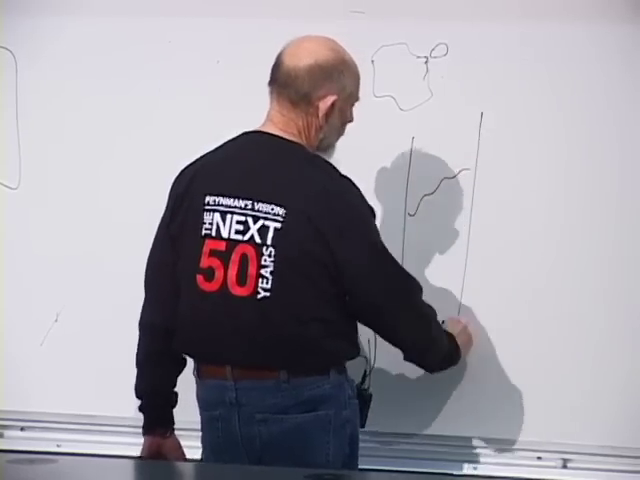
\includegraphics[width=0.72\textwidth]{lecture_06_figure_03.png}
\caption{Các phác họa hoàn chỉnh về quá trình trao đổi trên bảng: một hằng ghép gắn tại điểm phát và lại gắn thêm một lần nữa tại điểm hấp thụ.}
\lectureframe{00:11:30.000}
\end{figure}

Trong phiên bản của lý thuyết dây, photon được thay bằng graviton và điện tích được thay bằng \(g_s\). Một hệ số đi kèm sự phát ra và một hệ số khác đi kèm sự hấp thụ, nên độ mạnh hấp dẫn tỉ lệ như \(g_s^2\).

Ở khoảng cách lớn, chính tương tác ấy phải tái tạo định luật lực Newton,
\begin{equation}
F_{\mathrm{grav}}\sim G_N\frac{M_1M_2}{r^2}.
\end{equation}
Các khối lượng và sự phụ thuộc nghịch đảo bình phương mô tả nguồn và sự lan truyền; điều cần ở đây là hằng ghép nhân với chúng.

\begin{figure}[htbp]
\centering
\begin{tikzpicture}[x=1cm,y=1cm]
  \node[font=\small\bfseries] at (1.8,3.55) {electromagnetism};
  \draw[line width=0.8pt] (0,0) -- (0,3);
  \draw[line width=0.8pt] (3.6,0) -- (3.6,3);
  \draw[line width=0.8pt] plot[smooth] coordinates {(0,1.5) (0.45,1.72) (0.9,1.28) (1.35,1.72) (1.8,1.28) (2.25,1.72) (2.7,1.28) (3.15,1.72) (3.6,1.5)};
  \node[below] at (0,1.42) {\(e\)};
  \node[below] at (3.6,1.42) {\(e\)};
  \node[font=\small] at (1.8,0.25) {exchange strength \(\propto e^2\)};
  \node[font=\small\bfseries] at (7.2,3.55) {string gravity};
  \draw[line width=0.8pt,rounded corners=6pt] (5.4,0) -- (5.2,0.7) -- (5.5,1.5) -- (5.25,2.3) -- (5.4,3);
  \draw[line width=0.8pt,rounded corners=6pt] (9,0) -- (9.2,0.7) -- (8.9,1.5) -- (9.15,2.3) -- (9,3);
  \draw[line width=0.8pt] plot[smooth] coordinates {(5.5,1.5) (5.95,1.72) (6.4,1.28) (6.85,1.72) (7.3,1.28) (7.75,1.72) (8.2,1.28) (8.65,1.72) (8.9,1.5)};
  \node[below] at (5.5,1.42) {\(g_s\)};
  \node[below] at (8.9,1.42) {\(g_s\)};
  \node[font=\small] at (7.2,0.25) {exchange strength \(\propto g_s^2\)};
\end{tikzpicture}
\caption{Phép tương tự bằng cách đếm hằng ghép. Mỗi đầu của lượng tử được trao đổi đóng góp một hệ số tương tác.}
\end{figure}

Nhận xét này gần như xác định hằng số Newton. Hằng ghép \(g_s\) là vô thứ nguyên, còn trong bốn chiều \(G_N\) có thứ nguyên là độ dài bình phương. Độ dài vi mô sẵn có là \(\ell_s\), do đó
\begin{equation}
G_N\sim g_s^2\ell_s^2.
\label{eq:l06-newton-string}
\end{equation}
Kết hợp điều này với Phương trình~\eqref{eq:l06-planck-area} ta được
\begin{equation}
\ell_p\sim g_s\ell_s.
\label{eq:l06-planck-string}
\end{equation}

\begin{figure}[htbp]
\centering
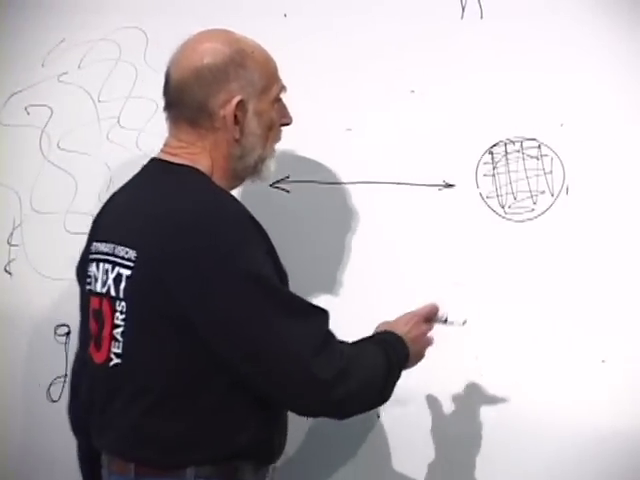
\includegraphics[width=0.72\textwidth]{lecture_06_figure_04.png}
\caption{Các hệ thức cơ bản được giữ lại trên bảng: \(\ell_p^2=G_N\) và \(\ell_p\sim g_s\ell_s\).}
\lectureframe{00:15:45.000}
\end{figure}

Phương trình~\eqref{eq:l06-newton-string} là hệ thức rút gọn được dùng xuyên suốt bài giảng này.\editorialnote{Trong lý thuyết dây đã compact hóa, hằng số Newton hiệu dụng bốn chiều còn phụ thuộc vào thể tích compact hóa và các quy ước hệ số cỡ một. Bài giảng lược bỏ những dữ liệu ấy để tách riêng luật tỉ lệ của phép tương ứng.}

\begin{classroomqa}
\audiencequestion{\(g_s\) lớn hơn hay nhỏ hơn một, và độ dài nào lớn hơn?\lecturetimestamp{00:16:00}}
\lecturerresponse{Ta làm việc ở ghép yếu, \(g_s<1\). Khi đó \(\ell_p\sim g_s\ell_s\) suy ra rằng độ dài dây lớn hơn độ dài Planck. Ghép mạnh đòi hỏi một mô tả khác và không cần ở đây.}
\end{classroomqa}

\section{Phép đếm cho hố đen}

Bỏ qua hằng số Boltzmann và các hệ số số học, entropy Bekenstein--Hawking là
\begin{equation}
S_{\mathrm{BH}}=\frac{A}{4G_N}sim\frac{A}{G_N}sim\frac{A}{\ell_p^2}.
\label{eq:l06-bh-area}
\end{equation}
Hệ số \(1/4\) là chính xác trong công thức bán cổ điển, nhưng nó sẽ không đóng vai trò nào trong lập luận theo luật tỉ lệ này.

\begin{classroomqa}
\audiencequestion{Chỉ số dưới ``BH'' có nghĩa là black hole hay Bekenstein--Hawking?\lecturetimestamp{00:16:51}}
\lecturerresponse{Với mục đích của ta, nó có thể gợi nhắc cả hai. Điều quan trọng là entropy bằng diện tích chân trời được đo theo các diện tích Planck.}
\end{classroomqa}

Đối với một hố đen Schwarzschild bốn chiều,
\begin{equation}
R_s=2G_NM,
\qquad
A=4\pi R_s^2.
\end{equation}
Bỏ qua \(2\) và \(4\pi\) như trong bài giảng,
\begin{align}
S_{\mathrm{BH}}
&\sim \frac{R_s^2}{G_N}
\sim \frac{(G_NM)^2}{G_N} \\
&\sim M^2G_N
\sim M^2\ell_p^2.
\label{eq:l06-bh-mass}
\end{align}
Đây là dạng ta sẽ so sánh với phép đếm của dây.

\section{Một dây dài như một bước đi ngẫu nhiên}

Hãy bắt đầu với một dây nhỏ và bơm năng lượng vào nó. Một dây kích thích mạnh điển hình không còn là một vòng gọn gàng. Nó trở thành một vật thể dài, rối mù, như dây câu sau khi ống cuộn bị rối tung. Mớ rối ấy có entropy vì một số lượng khổng lồ cấu hình trông giống nhau ở mức vĩ mô.

Để đếm chúng, hãy thay không gian bằng một mạng mà các link có độ dài \(\ell_s\). Các site là các đỉnh, các link là các đoạn thẳng, và các ô vuông cơ bản là các plaquette. Một dây được biểu diễn bằng một dãy liên thông các link. Mô hình này có chủ ý là thô sơ, nhưng phép đếm trạng thái tăng theo hàm mũ của nó nắm bắt được luật tỉ lệ mong muốn.

\begin{figure}[htbp]
\centering
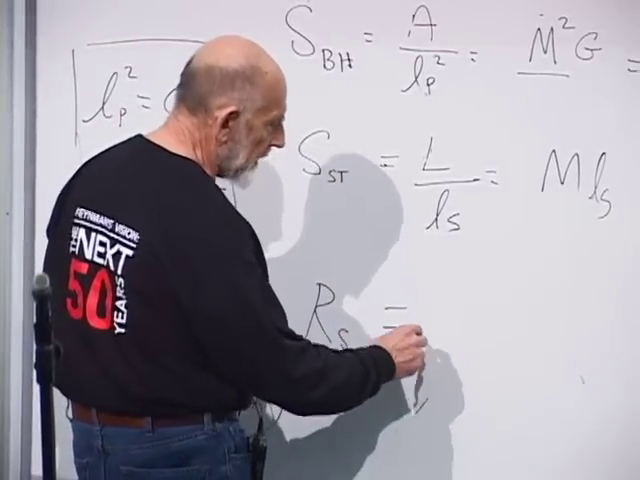
\includegraphics[width=0.72\textwidth]{lecture_06_figure_05.png}
\caption{Mô hình mạng hai chiều. Đoạn màu xanh đánh dấu một bước của dây; bốn khả năng tiếp diễn được đếm tại mỗi site.}
\lectureframe{00:23:50.000}
\end{figure}

\begin{classroomqa}
\audiencequestion{Có bao nhiêu lựa chọn ở mỗi bước của bước đi mô hình?\lecturetimestamp{00:22:43}}
\lecturerresponse{Là bốn trên mạng vuông, vì cho phép quay lui ngay lập tức. Trong ba chiều sẽ là sáu. Một mạng khác sẽ thay đổi con số thông thường, nhưng không thay đổi sự thật rằng số bước đi tăng theo hàm mũ với số link.}
\end{classroomqa}

Nếu dây có \(n\) link, thì phép đếm mô hình hai chiều là
\begin{equation}
\Omega_n\sim4^n.
\label{eq:l06-walk-count}
\end{equation}
Có một bước đi thẳng ngoại lệ, nhưng đó chỉ là một trạng thái trong \(4^n\). Một bước đi điển hình gấp khúc lặp đi lặp lại và chiếm một khối cầu rối. Với \(n\) lớn, hầu như mọi cấu hình được sinh ngẫu nhiên đều giống nhau về mặt định tính.

Entropy là logarit của số cấu hình không thể phân biệt ở mức vĩ mô:
\begin{equation}
S_{\mathrm{st}}=\log\Omega_n\sim n\log4\sim n.
\label{eq:l06-string-entropy-n}
\end{equation}

\begin{classroomqa}
\audiencequestion{Vì sao entropy lại tỉ lệ với \(n\) chứ không phải với \(4^n\)?\lecturetimestamp{00:25:39}}
\lecturerresponse{Entropy là logarit của số trạng thái. Do đó \(\log(4^n)=n\log4\), còn hệ số \(\log4\) là một hằng số cỡ một mà ta sẽ lược bỏ.}
\end{classroomqa}

Nếu \(L\) là độ dài đường cong thu được khi đi dọc theo dây từ đầu này đến đầu kia, thì
\begin{equation}
n=\frac{L}{\ell_s},
\qquad
S_{\mathrm{st}}\sim\frac{L}{\ell_s}.
\label{eq:l06-string-entropy-length}
\end{equation}
Ở đây \(L\) không phải là đường kính của khối rối. Nó là quãng đường dài hơn nhiều được đo dọc theo dây.

Tiếp theo ta đổi từ độ dài đường cong sang khối lượng. Với \(c=\hbar=1\), khối lượng có thứ nguyên là nghịch đảo của độ dài. Vì vậy một link cỡ dây mang khối lượng cỡ
\begin{equation}
m_{\mathrm{link}}\sim\frac{1}{\ell_s}.
\label{eq:l06-link-mass}
\end{equation}

\begin{classroomqa}
\audiencequestion{Vì sao khối lượng của một link phải tỉ lệ như \(1/\ell_s\)?\lecturetimestamp{00:29:20}}
\lecturerresponse{Trong các đơn vị này, khối lượng là nghịch đảo của độ dài, và \(\ell_s\) là độ dài sẵn có duy nhất. Tương đương, sức căng dây cỡ \(1/\ell_s^2\) nhân với độ dài link \(\ell_s\) cho cùng kết quả.}
\end{classroomqa}

Khi đó toàn bộ dây có
\begin{equation}
M\sim n m_{\mathrm{link}}
\sim\frac{n}{\ell_s}
\sim\frac{L}{\ell_s^2},
\qquad
L\sim M\ell_s^2.
\label{eq:l06-string-mass}
\end{equation}
Thế vào Phương trình~\eqref{eq:l06-string-entropy-length} ta được
\begin{equation}
S_{\mathrm{st}}\sim M\ell_s.
\label{eq:l06-string-entropy-mass}
\end{equation}
Bước đi trên mạng bỏ qua các ràng buộc của mặt thế giới và các hệ số số học, nhưng sự tăng theo hàm mũ của phổ dây kích thích mạnh cho cùng luật tỉ lệ dẫn đầu này.\editorialnote{Cấu trúc bước đi ngẫu nhiên là một mẹo ghi nhớ cho mật độ trạng thái của dây ở mức kích thích cao, chứ không phải một phép rời rạc hóa theo nghĩa đen của một dây cơ bản.}

\section{Sự không khớp mở đầu cho lập luận}

Giờ đây hai kết quả là
\begin{equation}
S_{\mathrm{BH}}\sim M^2\ell_p^2,
\qquad
S_{\mathrm{st}}\sim M\ell_s.
\label{eq:l06-two-entropies}
\end{equation}
Chúng giống nhau, nhưng không bằng nhau khi khối lượng cố định và hằng ghép tùy ý. Biểu thức của hố đen là bậc hai theo \(M\); biểu thức của dây là tuyến tính. Không thể đơn giản tuyên bố một dây nóng là hố đen mà không giải thích hai miền đó gặp nhau như thế nào.

\begin{figure}[htbp]
\centering
\includegraphics[width=0.78\textwidth]{lecture_06_figure_06.png}
\caption{Phép so sánh trên bảng không bị che khuất: entropy hố đen ở trên, entropy dây dài ở dưới, với các hệ thức Planck--dây được giữ lại ở bên trái.}
\lectureframe{00:33:20.000}
\end{figure}

Đây là chỗ lớp học tạm dừng. Sự hồi hộp này có ích: sự không khớp không phải là thất bại của ý tưởng, mà là manh mối cho thấy phải so sánh cùng một trạng thái trong khi thay đổi độ mạnh của hấp dẫn.

\section{Xoay núm điều chỉnh hằng ghép}

Giữ \(\ell_s\) cố định và hình dung rằng \(g_s\) có thể thay đổi. Tại \(g_s=0\), dây không tách cũng không nhập và hấp dẫn biến mất vì \(G_N\sim g_s^2\ell_s^2\). Khi đó một trạng thái có năng lượng đủ lớn là một dây dài tương tác yếu.

Tăng \(g_s\) từ từ. Các tương tác của dây trở nên khả dĩ và, quan trọng hơn đối với lập luận hiện tại, hấp dẫn mạnh lên.

\begin{classroomqa}
\audiencequestion{Khi \(g_s\) tăng, liệu hiệu ứng đầu tiên có đơn giản chỉ là dây tách thành những dây ngắn hơn không?\lecturetimestamp{00:36:29}}
\lecturerresponse{Sự tách và nhập trở nên khả dĩ, nhưng hãy giữ \(\ell_s\) cố định và theo dõi trạng thái entropy cao. Hiệu ứng trung tâm là \(G_N\) tăng lên, nên tự hấp dẫn của dây dài kéo khối rối co vào trong.}
\end{classroomqa}

Vật thể co lại và trở nên đậm đặc hơn. Thế năng hấp dẫn của nó là âm, nên sự co lại làm giảm tổng năng lượng của nó và do đó làm giảm khối lượng.

\begin{classroomqa}
\audiencequestion{Năng lượng tăng hay giảm khi tự hấp dẫn kéo dây lại với nhau?\lecturetimestamp{00:37:48}}
\lecturerresponse{Nó giảm. Năng lượng liên kết trở nên âm hơn. Khối lượng dọc theo quá trình đó không nhất thiết phải giữ cố định dù ta vẫn tiếp tục theo dõi cùng một trạng thái.}
\end{classroomqa}

Cuối cùng, kích thước của vật trở nên cùng bậc với bán kính Schwarzschild của nó. Vượt quá điểm đó, mô tả lỗ đen là cách mô tả tự nhiên. Một kích thích ban đầu lớn hơn đạt tới điều kiện này ở hằng số liên kết nhỏ hơn, vì một vật có khối lượng lớn hơn cần độ mạnh hấp dẫn nhỏ hơn để hình thành chân trời.

\begin{figure}[htbp]
\centering
\resizebox{0.95\linewidth}{!}{%
\begin{tikzpicture}[x=1cm,y=1cm,>=Latex]
  \draw[->,line width=0.9pt] (0,0) -- (11,0) node[right] {increasing \(g_s\)};
  \node[draw,rounded corners,align=center,minimum width=2.6cm,minimum height=1.15cm] at (1.8,1.5) {long excited string\\weak self-gravity};
  \node[draw,rounded corners,align=center,minimum width=2.6cm,minimum height=1.15cm] at (5.5,1.5) {correspondence point\\\(R_s\sim\ell_s\)};
  \node[draw,circle,align=center,minimum size=1.8cm] at (9.3,1.5) {black\\hole};
  \draw[->,line width=0.8pt] (3.15,1.5) -- (4.1,1.5) node[midway,above,font=\small] {contracts};
  \draw[->,line width=0.8pt] (6.9,1.5) -- (8.25,1.5);
  \node[font=\small,align=center] at (5.5,-0.65) {same family of states followed slowly;\\binding energy and mass may change};
\end{tikzpicture}
}
\caption{Quỹ đạo tương ứng khi giữ \(\ell_s\) cố định. Đảo ngược mũi tên đưa trạng thái lỗ đen trở lại trạng thái dây dài.}
\end{figure}

\begin{classroomqa}
\audiencequestion{Ta có nên hình dung \(g_s\) nằm giữa 0 và 1 không?\lecturetimestamp{00:40:18}}
\lecturerresponse{Có. Lập luận vẫn nằm trong miền liên kết yếu. Nếu \(g_s\) rất nhỏ, thì trạng thái đó phải có khối lượng lớn tương ứng trước khi trở thành lỗ đen. Chúng ta không cần đi vào miền \(g_s>1\) được kiểm soát kém.}
\end{classroomqa}

Sự thay đổi chậm là thuận nghịch trong thí nghiệm tưởng tượng này.

\begin{classroomqa}
\audiencequestion{Nếu ta hạ hằng số liên kết trở lại cho đến khi hấp dẫn không còn có thể giữ lỗ đen gắn kết nữa, thì nó trở thành gì?\lecturetimestamp{00:41:37}}
\lecturerresponse{Một dây dài. Khi hấp dẫn triệt tiêu, mọi thứ trong cách xây dựng này đều phải được mô tả bằng các trạng thái dây. Xoay núm điều chỉnh theo một chiều sẽ ánh xạ dây thành lỗ đen; xoay ngược lại sẽ ánh xạ lỗ đen thành dây.}
\end{classroomqa}

Với tổng năng lượng cố định và trong một thể tích cố định, cấu hình entropy cao chiếm ưu thế về cơ bản là một dây dài chứ không phải một số lượng khổng lồ các dây ngắn. Mệnh đề đó không được suy ra ở đây. Đó là kết quả của cơ học thống kê của các dây gần chế độ Hagedorn và sẽ được quay lại sau.

\section{Những gì người quan sát bên ngoài thấy}

Dây ở đâu khi vật được mô tả là một lỗ đen? Trong mô tả từ bên ngoài, nó không đột ngột biến mất. Thời gian Schwarzschild đẩy sự băng qua biểu kiến tới thời điểm muộn tùy ý, nên các bậc tự do dạng dây được biểu diễn như đang tích tụ trên hoặc gần chân trời.

\begin{figure}[htbp]
\centering
\includegraphics[width=0.72\textwidth]{lecture_06_figure_07.png}
\caption{So sánh trên bảng giữa một chân trời vĩ mô, nơi cấu trúc ở thang dây chỉ là một lớp mờ mỏng, và một chân trời nhỏ hơn có bán kính tiến gần tới thang kích thước vòng.}
\lectureframe{00:45:30.000}
\end{figure}

Khi \(R_s\gg\ell_s\), lỗ đen là vĩ mô và cấu trúc ở thang dây chỉ là một lớp mỏng so với bán kính chân trời. Khi bán kính giảm xuống gần \(\ell_s\), sự phân biệt giữa một lỗ đen trơn và một dây mở rộng mất đi ý nghĩa. Đây là mô tả bên ngoài theo chân trời kéo giãn; không nên nhầm nó với một khẳng định độc lập với tọa độ rằng vật chất rơi vào không bao giờ đi qua một chân trời chính quy.\editorialnote{Bài giảng dùng mô tả bên ngoài quen thuộc trong nguyên lý bổ sung lỗ đen. Cụm ``trên chân trời'' chỉ các bậc tự do được phân giải trong mô tả từ bên ngoài, chứ không phải một suy dẫn riêng về vị trí hiệp biến của chúng.}

Sự chuyển tiếp xảy ra khi
\begin{equation}
R_s\sim\ell_s.
\label{eq:l06-correspondence-radius}
\end{equation}
Bên dưới thang dây, hình học Schwarzschild không thể phân giải cấu trúc được cho là nâng đỡ nó. Các vòng dao động rời khỏi chân trời lẽ ra sẽ có, và trạng thái ấy đúng hơn nên được gọi là một dây.

\section{Điểm tương ứng}

Dùng \(R_s\sim G_NM\) trong Phương trình~\eqref{eq:l06-correspondence-radius}:
\begin{equation}
G_NM\sim\ell_s.
\end{equation}
Sau đó thế \(G_N\sim g_s^2\ell_s^2\):
\begin{equation}
M g_s^2\ell_s^2\sim\ell_s,
\qquad
M g_s^2\ell_s\sim1.
\label{eq:l06-correspondence-condition}
\end{equation}

\begin{figure}[htbp]
\centering
\includegraphics[width=0.72\textwidth]{lecture_06_figure_08.png}
\caption{Phần đại số hoàn chỉnh của sự chuyển tiếp trên bảng: \(R_s\sim\ell_s\) dẫn tới điều kiện vô thứ nguyên được đóng khung \(Mg_s^2\ell_s\sim1\).}
\lectureframe{00:49:50.000}
\end{figure}

Một người nghe nhận ra điều kiện này đang chuẩn bị cho điều gì. Tại điểm tương ứng,
\begin{align}
S_{\mathrm{BH}}
&\sim M^2\ell_p^2
\sim M^2g_s^2\ell_s^2 \\
&=(M\ell_s)(Mg_s^2\ell_s)
\sim M\ell_s
\sim S_{\mathrm{st}}.
\label{eq:l06-entropy-preview}
\end{align}

\begin{classroomqa}
\audiencequestion{Các phương trình đã ngụ ý rằng entropy của lỗ đen và của dây trở nên bằng nhau hay chưa?\lecturetimestamp{00:50:18}}
\lecturerresponse{Đúng. Đó chính là hướng mà phép tính đang đi tới. Các thành phần đã được đặt lên bảng, nhưng bài giảng hoãn việc lắp ghép đầy đủ chúng lại để có thể xem xét cẩn thận logic của phép tương ứng.}
\end{classroomqa}

Phương trình~\eqref{eq:l06-entropy-preview} là bản xem trước đại số một dòng hàm ẩn trong phần trao đổi đó. Nó xác lập quy luật tỉ lệ, không phải hệ số chính xác \(1/4\). Những sự khớp vi mô chính xác đòi hỏi các lỗ đen được kiểm soát tốt hơn và các cấu trúc dây chi tiết hơn.\editorialnote{Bài giảng dừng lại trước khi trình bày Phương trình~\eqref{eq:l06-entropy-preview} như một phép suy dẫn hoàn chỉnh. Nó được viết ra ở đây vì người nghe đã nêu đích danh sự bằng nhau ấy và mọi hệ thức cần thiết đều đã xuất hiện.}

\section{Vì sao entropy có thể được chuyển qua}

Còn lại một thành phần logic nữa. Giả sử một tham số điều khiển, chẳng hạn như từ trường hay \(g_s\), được biến thiên đủ chậm trong khi hệ được cô lập và tiến hóa là thuận nghịch. Năng lượng, kích thước và mức độ liên kết có thể thay đổi, nhưng entropy được bảo toàn:
\begin{equation}
\Delta S=0.
\label{eq:l06-adiabatic-entropy}
\end{equation}
Bài giảng nối điều này với sự bảo toàn thông tin. Entropy đo lượng thông tin bị che khuất bởi một mô tả thô hoá; một sự thay đổi chậm, thuận nghịch của Hamiltonian sắp xếp lại các trạng thái mà không xóa đi thông tin đó.

\begin{classroomqa}
\audiencequestion{Entropy không đổi có đòi hỏi rằng đường đi phải tránh một chuyển pha không?\lecturetimestamp{00:54:01}}
\lecturerresponse{Có, phải có thể theo dõi trạng thái một cách liên tục. Một hệ hữu hạn không có chuyển pha nhiệt động học phi giải tích đúng nghĩa kiểu thể tích vô hạn, và nếu sự thay đổi đủ chậm thì phép tương ứng có thể được xem như một sự chuyển tiếp trơn.}
\end{classroomqa}

Ở đây, đoạn nhiệt được dùng theo nghĩa mạnh hơn, gần tĩnh và thuận nghịch. Một quá trình đoạn nhiệt nhưng không thuận nghịch có thể sinh entropy; sự chậm và khả năng theo dõi trạng thái là thiết yếu.\editorialnote{Mệnh đề nhiệt động học \(\Delta S=0\) đòi hỏi một đường đi đoạn nhiệt thuận nghịch. Về mặt cơ học lượng tử, ý tưởng tương ứng là bám theo cùng một tập trạng thái khi một tham số thay đổi mà không có các chuyển mức mất kiểm soát.}

\begin{classroomqa}
\audiencequestion{Vì sao một dây dài lại có entropy lớn hơn vài dây ngắn hơn mang cùng tổng khối lượng?\lecturetimestamp{00:54:44}}
\lecturerresponse{Điều đó trái trực giác, nhưng phép đếm tường minh các trạng thái năng lượng cao ưu ái một thành phần dây dài trong một thể tích cố định. Chứng minh được để lại sau; đối với lập luận hiện tại, ta chỉ cần rằng lỗ đen được ánh xạ vào sector dây entropy cực đại, chứ không phải vào một khí loãng gồm rất nhiều dây ngắn.}
\end{classroomqa}

Vì vậy, chiến lược thực hiện là:
\begin{enumerate}
\item Bắt đầu với một lỗ đen khối lượng \(M_0\) ở hằng số liên kết \(g_{s,0}\).
\item Giảm \(g_s\) từ từ trong khi bám theo cùng một họ trạng thái entropy cao.
\item Dừng ở \(R_s\sim\ell_s\), nơi mô tả lỗ đen chuyển thành mô tả dây dài.
\item Đếm các trạng thái dây bằng \(S_{\mathrm{st}}\sim M\ell_s\).
\item Mang entropy đó trở lại dọc theo đường đi thuận nghịch tới lỗ đen ban đầu.
\end{enumerate}

\begin{figure}[htbp]
\centering
\includegraphics[width=0.72\textwidth]{lecture_06_figure_09.png}
\caption{Nguyên lý được giữ lại trên bảng trong khi trình bày chiến lược: một sự thay đổi đoạn nhiệt của \(g_s\) không làm thay đổi \(S\).}
\lectureframe{00:56:40.000}
\end{figure}

Lý thuyết dây đã cho ra những phép đếm entropy sắc nét hơn nhiều cho các lỗ đen mang điện, quay, siêu đối xứng, gần cực trị và ở số chiều cao hơn. Thảo luận về Schwarzschild trung hòa ở đây là lập luận tương ứng gần đúng: nó xác định sự phụ thuộc theo tham số của mật độ trạng thái và sự chuyển tiếp vật lý, chứ không phải một độ suy biến được bảo vệ một cách chính xác.\editorialnote{Sự phù hợp chính xác là mạnh nhất đối với các lỗ đen đặc biệt mà phép đếm trạng thái của chúng được bảo vệ khi hằng số liên kết thay đổi. Bài giảng này chủ ý trình bày phiên bản đơn giản nhất ở mức bậc độ lớn.}

\begin{classroomqa}
\audiencequestion{Khi hấp dẫn bị tắt đi, trạng thái đó có thể trở thành hai dây thay vì đúng một dây không?\lecturetimestamp{00:58:25}}
\lecturerresponse{Có một xác suất hữu hạn để xuất hiện một số ít dây dài, và việc có hai thay vì một không làm thay đổi quy luật tỉ lệ entropy ở bậc dẫn đầu. Điều sẽ làm thay đổi lập luận là sự phân mảnh thành một đám khí khổng lồ gồm các dây ngắn; phép đếm thống kê ở năng lượng cao không ưu tiên kết cục đó.}
\end{classroomqa}

Lỗ đen là lượng entropy lớn nhất có thể nhồi vào một vùng, và dây dài là trạng thái entropy cao tương ứng khi bỏ hấp dẫn đi. Hai mô tả ấy giờ đã được nối với nhau, nhưng vẫn chưa được phát triển thành một phép tính chính xác. Bước tiếp theo là lặp lại phần đại số một cách cẩn thận và hỏi phép tương ứng có thể được tin cậy đến mức nào.

\chapter{Entropy lỗ đen, toàn ảnh và không gian de Sitter}

\lectureoverview{Chúng ta hoàn tất lập luận tương ứng đã bắt đầu ở bài giảng trước. Một dây kích thích mạnh có entropy tỉ lệ với khối lượng của nó, còn một lỗ đen Schwarzschild có entropy tỉ lệ với diện tích của nó. Hai công thức này được nối với nhau không phải bằng cách đồng nhất một lỗ đen tự hấp dẫn mạnh với một dây tự do, mà bằng cách biến thiên chậm hằng số ghép dây cho đến khi hai mô tả gặp nhau. Khi đó định luật diện tích dẫn một cách tự nhiên đến nguyên lý toàn ảnh, và phần cuối của bài giảng giới thiệu không gian giãn nở cùng hình học de Sitter, với chân trời của nó sẽ được khảo sát tiếp theo.}

\section{Trở lại bài toán đếm}

Có một điểm còn bỏ ngỏ trong phép đếm dây dài. Nếu một tổng chiều dài cố định được chia cho một số dây, các dây giống hệt nhau có cùng độ dài là không thể phân biệt được. Tuy vậy, vị trí của chúng trong hộp vẫn là một phần của trạng thái, và hộp được chọn có kích thước xấp xỉ vùng mà một dây dài đơn lẻ tương ứng chiếm giữ.

\begin{classroomqa}
\audiencequestion{Các dây ngắn có được phân biệt với nhau không, và vị trí của chúng có được tính không?\lecturetimestamp{00:00:37}}
\lecturerresponse{Các dây có cùng các tính chất là không thể phân biệt được, nhưng vị trí của chúng trong hộp thì được tính. Việc so sánh được thực hiện ở thể tích cố định, được chọn sao cho khớp với vùng mà dây dài chiếm giữ.}
\end{classroomqa}

Với điểm đó đã được làm rõ, ta có thể nêu mục tiêu. Chúng ta sẽ tập hợp một danh sách ngắn các phương trình và dùng chúng để suy ra quy luật tỉ lệ của entropy lỗ đen. Không cần đến tích phân hay tổng vô hạn nào. Khó khăn không nằm ở đại số; nó nằm ở chỗ biết những đại lượng nào có thể đem so sánh và ở giai đoạn nào của lập luận.

\section{Đơn vị tự nhiên và diện tích Planck}

Đặt
\begin{equation}
c=\hbar=1,
\label{eq:l07-natural-units}
\end{equation}
nhưng vẫn giữ tường minh hằng số Newton. Hệ quả đầu tiên là thời gian và độ dài có cùng đơn vị. Hệ thức photon
\begin{equation}
E=\frac{\hbar c}{\lambda}
\end{equation}
và hệ thức khối lượng–năng lượng \(E=mc^2\) khi đó suy ra
\begin{equation}
[M]=L^{-1}.
\label{eq:l07-mass-dimension}
\end{equation}
Vì thế, khối lượng có thể được biểu diễn như nghịch đảo của một độ dài.

\begin{figure}[htbp]
\centering
\includegraphics[width=0.62\textwidth]{lecture_07_figure_02.png}
\caption{Quy ước đơn vị tự nhiên ở đầu lập luận thứ nguyên. Công thức năng lượng được hoàn chỉnh trong các phương trình bên trên.}
\lectureframe{00:03:27.900}
\end{figure}

Để xác định đơn vị của \(G_N\), hãy chỉ dùng gia tốc Newton như một phép hạch toán thứ nguyên:
\begin{equation}
a\sim\frac{G_NM}{R^2}.
\end{equation}
Vì \(T\) và \(L\) có cùng đơn vị, nên \([a]=L/T^2=L^{-1}\). Kết hợp với Phương trình~\eqref{eq:l07-mass-dimension}, ta được
\begin{equation}
[G_N]=L^2.
\end{equation}
Trong các đơn vị này, hằng số Newton là một diện tích. Định nghĩa độ dài Planck bởi
\begin{equation}
G_N=\ell_p^2,
\label{eq:l07-planck-area}
\end{equation}
ta hiểu ngay vì sao \(A/G_N=A/\ell_p^2\) là không thứ nguyên: nó đo một diện tích theo đơn vị diện tích Planck.

\section{Hằng số ghép dây và độ mạnh của hấp dẫn}

Bây giờ hấp dẫn phải được diễn đạt bằng ngôn ngữ dây. Hình dung hữu ích là một quá trình trao đổi. Khi một dây tự cắt qua chính nó, nó có thể tách ra rồi nhập lại. Một vòng dây kín nhỏ có thể được một vật phát ra và một vật khác hấp thụ; khi kích thích ấy là một graviton, quá trình đó làm trung gian cho hấp dẫn. Một thừa số tương tác xuất hiện ở lúc phát ra và một thừa số khác ở lúc hấp thụ, nên cường độ trao đổi chứa \(g_s^2\).

Hằng số ghép \(g_s\) là không thứ nguyên. Chính xác hơn, đó là hằng số ghép ở cấp biên độ, còn xác suất hay tốc độ thì bắt đầu ở bậc \(g_s^2\).\editorialnote{Trong bài giảng đôi khi \(g_s\) được gọi là một xác suất rồi được đính chính thành căn bậc hai của một xác suất. Hằng số ghép nhiễu loạn thuộc cấp biên độ.} Vì \(G_N\) có thứ nguyên diện tích, vẫn còn thiếu một thang độ dài. Độ dài dây cơ bản \(\ell_s\), là thang của một dao động cơ bản của dây, cung cấp nó:
\begin{equation}
G_N\sim g_s^2\ell_s^2,
\qquad
\ell_p\sim g_s\ell_s.
\label{eq:l07-planck-string}
\end{equation}

\begin{figure}[htbp]
\centering
\includegraphics[width=0.72\textwidth]{lecture_07_figure_05.png}
\caption{Hệ thức ghép trên bảng: \(G_N=\ell_p^2\) và \(g_s^2\ell_s^2\sim\ell_p^2\).}
\lectureframe{00:12:15.000}
\end{figure}

Ở ghép yếu, \(g_s\ll1\), độ dài Planck nhỏ hơn nhiều so với độ dài dây. Giảm \(g_s\) sẽ làm hấp dẫn yếu đi trong khi giữ cố định thang dây sơ cấp.\editorialnote{Đối với một lý thuyết hiệu dụng bốn chiều, dữ liệu compact hóa và các quy ước số cũng đi vào \(G_N\). Chúng được giữ cố định và được lược bỏ trong lập luận về quy luật tỉ lệ này.}

\section{Đếm một dây dài}

Entropy đếm số lựa chọn sơ cấp cần thiết để xác định một trạng thái. Hãy thay một dây kích thích mạnh bằng một đường đi trên mạng vuông. Ở mỗi đỉnh, đoạn tiếp theo có thể chỉ theo một trong bốn hướng. Việc mô tả lựa chọn sơ cấp ấy như một quyết định bốn ngả hay hai quyết định nhị phân chỉ làm thay đổi một hằng số bậc một. Điều quan trọng là số bước.

Nếu \(L\) là chiều dài đường cong của dây và mỗi bước có độ dài \(\ell_s\), thì cần
\begin{equation}
N=\frac{L}{\ell_s}
\end{equation}
bước. Số đường đi tăng theo hàm mũ, về mặt sơ đồ là \(\Omega_N\sim q^N\) với \(q\) cỡ đơn vị, và do đó
\begin{equation}
S_{\mathrm{str}}=\log\Omega_N\sim N\sim\frac{L}{\ell_s}.
\label{eq:l07-string-entropy-length}
\end{equation}

\begin{figure}[htbp]
\centering
\includegraphics[width=0.68\textwidth]{lecture_07_figure_03.png}

\vspace{0.7em}
\begin{tikzpicture}[scale=0.82]
  \draw[step=0.8cm,gray!45,thin] (0,0) grid (6.4,4.0);
  \draw[very thick,blue!60!black]
    (0.8,0.8)--(1.6,0.8)--(1.6,1.6)--(2.4,1.6)--(2.4,2.4)--
    (3.2,2.4)--(3.2,1.6)--(4.0,1.6)--(4.0,2.4)--(4.8,2.4)--
    (4.8,3.2)--(5.6,3.2);
  \draw[<->,thick] (0.8,-0.35)--(1.6,-0.35);
  \node[below] at (1.2,-0.35) {step \(\ell_s\)};
  \node[align=center] at (8.1,2.0) {\(N=L/\ell_s\) steps\\[0.3em]\(S_{\mathrm{str}}\sim N\)};
\end{tikzpicture}
\caption{Mô hình mạng trên bảng và cách diễn giải đã được làm gọn của nó theo bước đi ngẫu nhiên. Chính chiều dài đường cong, chứ không phải đường kính của búi rối, quyết định số lựa chọn.}
\lectureframe{00:17:20.000}
\end{figure}

Khối lượng được đếm từ chính các đoạn sơ cấp ấy. Một đoạn có độ dài \(\ell_s\) có thang khối lượng
\begin{equation}
m_{\mathrm{seg}}\sim\frac{1}{\ell_s}.
\end{equation}

\begin{classroomqa}
\audiencequestion{Đoạn sơ cấp có đang được gán độ dài \(\ell_s\) không?\lecturetimestamp{00:18:56}}
\lecturerresponse{Có. Độ dài đặc trưng của nó là \(\ell_s\), nên trong đơn vị tự nhiên khối lượng đặc trưng của nó là \(1/\ell_s\).}
\end{classroomqa}

Cộng \(L/\ell_s\) khối lượng đoạn lại cho ta
\begin{equation}
M\sim\frac{L}{\ell_s}\frac{1}{\ell_s}
=\frac{L}{\ell_s^2},
\qquad
L\sim M\ell_s^2.
\label{eq:l07-string-mass}
\end{equation}
Động năng và thế năng của dây dao động đã được nén vào hệ thức tỉ lệ này; một cách xử lý cơ học thống kê chi tiết cũng cho cùng sự phụ thuộc. Thế vào Phương trình~\eqref{eq:l07-string-entropy-length} ta thu được công thức phía dây mà ta sẽ cần:
\begin{equation}
S_{\mathrm{str}}\sim M\ell_s.
\label{eq:l07-string-entropy-mass}
\end{equation}

\begin{figure}[htbp]
\centering
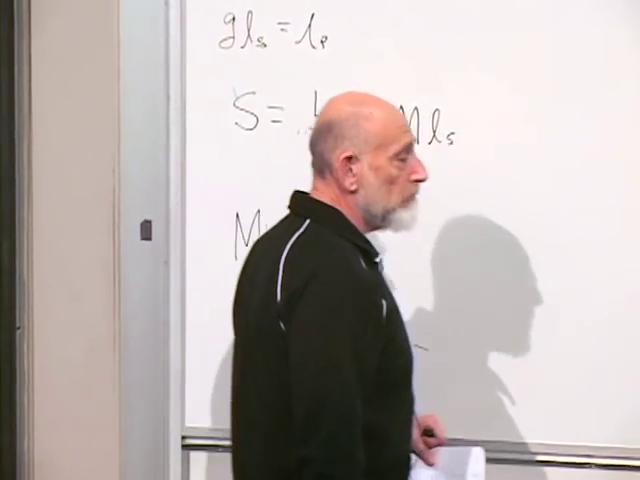
\includegraphics[width=0.66\textwidth]{lecture_07_figure_04.png}
\caption{Cột phía dây được tập hợp trước khi so sánh: \(\ell_p\sim g_s\ell_s\), \(S_{\mathrm{str}}\sim L/\ell_s\sim M\ell_s\) và \(M\sim L/\ell_s^2\).}
\lectureframe{00:21:57.800}
\end{figure}

\section{Vì sao một dây tự do vẫn chưa phải là một lỗ đen}

Ở phía hấp dẫn, công thức bán cổ điển chính xác là
\begin{equation}
S_{\mathrm{BH}}=\frac{A}{4G_N}.
\label{eq:l07-bh-exact}
\end{equation}

\begin{classroomqa}
\audiencequestion{Hệ số số nào nằm ở mẫu số?\lecturetimestamp{00:23:28}}
\lecturerresponse{Là 4. Lập luận tương ứng sẽ khôi phục quy luật tỉ lệ nhưng quá thô để xác định đúng hệ số chính xác đó.}
\end{classroomqa}

Đối với một lỗ đen Schwarzschild bốn chiều,
\begin{equation}
R_s=2G_NM,
\qquad
A=4\pi R_s^2.
\end{equation}
Bỏ qua các hệ số số như bài giảng vẫn làm,
\begin{align}
S_{\mathrm{BH}}
&\sim\frac{A}{G_N}
\sim\frac{(G_NM)^2}{G_N} \\
&\sim M^2G_N
\sim M^2\ell_p^2.
\label{eq:l07-bh-scaling}
\end{align}

\begin{figure}[htbp]
\centering
\includegraphics[width=0.72\textwidth]{lecture_07_figure_06.png}
\caption{Phép so sánh đã hoàn tất trên bảng: entropy dây là một độ dài tính theo đơn vị dây, còn entropy lỗ đen là một diện tích tính theo đơn vị Planck.}
\lectureframe{00:25:35.000}
\end{figure}

Sự giống nhau giữa Phương trình~\eqref{eq:l07-string-entropy-mass} và \eqref{eq:l07-bh-scaling} là gợi ý đáng chú ý, nhưng chúng không phải cùng một công thức. Sẽ là sai nếu chỉ đơn giản gọi lỗ đen ban đầu là một dây tự do rồi thế vào. Phép đếm dây tự do bỏ qua tương tác hút giữa các phần của dây, chính là tương tác nén dây thành một lỗ đen và hạ thấp tổng năng lượng của nó thông qua năng lượng liên kết âm.

Một ngôi sao khiến sai lầm ấy trở nên quen thuộc. Một chất khí nóng có khối lượng sao đặt trong một cái hộp quá lớn không phải là mô hình của một ngôi sao, ngay cả ở cùng nhiệt độ. Tự hấp dẫn làm thay đổi kích thước cân bằng và quan hệ giữa năng lượng với entropy. Việc lần theo mọi tự tương tác của một dây dài sẽ rất khó, nên ta sẽ tránh làm điều đó.

\begin{classroomqa}
\audiencequestion{Nếu một vòng nhỏ rời khỏi một dây dài, entropy của nó giảm. Vậy trao đổi graviton có làm giảm entropy của hệ hấp dẫn không?\lecturetimestamp{00:28:48}}
\lecturerresponse{Không phải trong quá trình trao đổi cân bằng đang được dùng ở đây. Các kích thích ảo được phát ra và hấp thụ theo cả hai chiều; hình vẽ minh họa đó không phải là sự mất đi theo nghĩa đen của một mảnh dây vĩnh viễn. Mục đích duy nhất hiện tại của nó là thiết lập hai thừa số ghép và do đó là sự phụ thuộc theo \(g_s^2\).}
\end{classroomqa}

\section{Trò chơi tương ứng đoạn nhiệt}

Thay vào đó, hãy bắt đầu ở nơi hấp dẫn có thể bỏ qua. Khi \(g_s\to0\), các dây cắt qua nhau mà không tách hay nhập, và lực hút do tự hấp dẫn biến mất. Tăng \(g_s\) trong khi giữ \(\ell_s\) cố định: hấp dẫn mạnh lên, một dây kích thích mạnh co lại, và rốt cuộc nó trở thành một lỗ đen. Vặn ngược núm điều chỉnh một cách chậm rãi thì lỗ đen phải trở về một trạng thái dây. Nó có thể trở thành một số nhỏ các dây dài, nhưng phép đếm năng lượng cao từ bài giảng trước nói rằng ngành trội chứa một dây dài chứ không phải một chất khí khổng lồ gồm các dây ngắn.

\begin{classroomqa}
\audiencequestion{Điều gì được giữ cố định khi hằng số ghép thay đổi?\lecturetimestamp{00:32:19}}
\lecturerresponse{Độ dài dây \(\ell_s\), và do đó thang khối lượng dây sơ cấp \(1/\ell_s\), được giữ cố định. Núm điều chỉnh làm thay đổi \(g_s\) và vì thế \(G_N\sim g_s^2\ell_s^2\).}
\end{classroomqa}

Sự thay đổi phải chậm, cô lập và thuận nghịch. Dưới những điều kiện đó, entropy là một bất biến đoạn nhiệt:
\begin{equation}
\Delta S=0.
\label{eq:l07-adiabatic}
\end{equation}
Chỉ chậm thôi là chưa đủ nếu xảy ra các chuyển tiếp tiêu tán hoặc không được kiểm soát. Ở đây ``đoạn nhiệt'' có nghĩa là có thể theo dõi liên tục cùng một họ trạng thái.\editorialnote{Đây là nghĩa nhiệt động học thuận nghịch của đoạn nhiệt. Một quá trình bất thuận nghịch có thể là đoạn nhiệt theo nghĩa không có dòng nhiệt mà vẫn tạo ra entropy.}

Gọi lỗ đen đích có khối lượng \(M_0\) và hằng số ghép \(g_{s,0}\). Trước khi dùng công thức diện tích mà ta đang tìm cách giải thích, phân tích thứ nguyên chỉ cho biết rằng entropy của một lỗ đen trung hòa, không quay là một hàm nào đó của tổ hợp không thứ nguyên
\begin{equation}
S_{\mathrm{BH}}=f(M\ell_p)
=f(Mg_s\ell_s).
\label{eq:l07-entropy-function}
\end{equation}
Vì vậy, khi giữ \(\ell_s\) cố định, một quỹ đạo đẳng entropy sẽ giữ
\begin{equation}
Mg_s=M_0g_{s,0}
\label{eq:l07-adiabat}
\end{equation}
không đổi, miễn là đi theo cùng một nhánh trạng thái.

Khi \(g_s\) giảm, năng lượng liên kết âm bị loại bỏ, nên khối lượng \(M\) tăng dọc theo quỹ đạo này. Cấu hình dây nền tảng cũng bớt bị liên kết chặt và lan rộng ra. Tuy nhiên, bán kính Schwarzschild hình thức ứng xử như \(R_s\sim Mg_s^2\ell_s^2\sim g_s\ell_s\) trên đường đoạn nhiệt và vì thế giảm.\editorialnote{Trong phần trình bày bằng lời, từ ``nở ra'' được dùng cho vật thể khi được giải phóng khỏi liên kết hấp dẫn. Không nên hiểu điều đó là bán kính Schwarzschild tăng dọc theo đường đoạn nhiệt suy ra ở trên.}

\begin{classroomqa}
\audiencequestion{Vật thể lớn lên hay co lại khi hấp dẫn yếu đi?\lecturetimestamp{00:36:28}}
\lecturerresponse{Cấu trúc dây của nó được giải phóng và nở ra, trong khi khối lượng của nó tăng vì năng lượng liên kết âm bị loại bỏ. Bán kính do công thức lỗ đen gán cho nó giảm xuống cho đến khi chạm thang dây, tại đó mô tả lỗ đen ấy không còn hữu ích nữa.}
\end{classroomqa}

\section{Hai đường cong và giao điểm của chúng}

Biểu diễn khối lượng theo trục đứng và hằng số ghép dây theo trục ngang. Phương trình~\eqref{eq:l07-adiabat} là một đường hyperbol, \(M\propto g_s^{-1}\).

\begin{classroomqa}
\audiencequestion{Loại đường cong nào có tích \(Mg_s\) không đổi?\lecturetimestamp{00:44:08}}
\lecturerresponse{Một đường hyperbol. Đó là đường đoạn nhiệt đi qua điểm đích \((g_{s,0},M_0)\).}
\end{classroomqa}

Đường cong thứ hai đánh dấu chỗ chuyển tiếp giữa hai mô tả. Một lỗ đen không còn có thể được phân giải như một hình học Schwarzschild thông thường một khi bán kính của nó nhỏ hơn một dao động sơ cấp của dây. Vì vậy ta ước lượng điểm tương ứng bằng
\begin{equation}
R_s\sim\ell_s.
\label{eq:l07-correspondence-radius}
\end{equation}
Dùng \(R_s\sim MG_N\) và Phương trình~\eqref{eq:l07-planck-string}, điều này trở thành
\begin{equation}
Mg_s^2\ell_s^2\sim\ell_s,
\qquad
Mg_s^2\sim\frac{1}{\ell_s}.
\label{eq:l07-transition-curve}
\end{equation}
Do đó, đường cong chuyển tiếp đi xuống theo \(M\propto g_s^{-2}\), dốc hơn đường đoạn nhiệt.

\begin{figure}[htbp]
\centering
\includegraphics[width=0.70\textwidth]{lecture_07_figure_07.png}

\vspace{0.6em}
\begin{tikzpicture}[x=1cm,y=0.78cm]
  \draw[->] (0.4,0.4)--(7.0,0.4) node[right] {\(g_s\)};
  \draw[->] (0.4,0.4)--(0.4,6.5) node[above] {\(M\)};
  \draw[thick,black] plot[smooth] coordinates {(1.0,5.6) (1.5,4.0) (2.2,2.9) (3.2,2.1) (4.6,1.55) (6.3,1.2)};
  \draw[very thick,red!70!black] plot[smooth] coordinates {(1.25,6.0) (1.55,4.55) (2.0,3.15) (2.7,2.0) (3.8,1.25) (5.8,0.78)};
  \fill (2.05,3.1) circle (2pt) node[above right] {\((g_{s,*},M_*)\)};
  \node[black,rotate=-17] at (4.75,1.9) {\(Mg_s=M_0g_{s,0}\)};
  \node[red!70!black,rotate=-25] at (4.45,0.95) {\(Mg_s^2=1/\ell_s\)};
  \node at (5.75,3.5) {black hole};
  \node at (1.15,1.25) {string};
\end{tikzpicture}
\caption{Đồ thị trên bảng và cách diễn giải đã được làm gọn của nó. Đường đoạn nhiệt màu đen cắt đường cong tương ứng màu đỏ dốc hơn tại điểm mà vật thể trở nên giống dây.}
\lectureframe{00:49:35.000}
\end{figure}

Tại giao điểm \((M_*,g_{s,*})\), hai phương trình là
\begin{align}
M_*g_{s,*} &= M_0g_{s,0}, \\
M_*g_{s,*}^2 &\sim \frac{1}{\ell_s}.
\end{align}
Bình phương phương trình thứ nhất rồi chia cho phương trình thứ hai:
\begin{equation}
M_*
\sim M_0^2g_{s,0}^2\ell_s.
\end{equation}
Nhân với \(\ell_s\),
\begin{equation}
M_*\ell_s
\sim M_0^2g_{s,0}^2\ell_s^2
\sim M_0^2G_{N,0}.
\label{eq:l07-crossover-result}
\end{equation}

\begin{figure}[htbp]
\centering
\includegraphics[width=0.68\textwidth]{lecture_07_figure_08.png}
\caption{Phần đại số chuyển tiếp đã hoàn tất, bao gồm \(M_*\ell_s=M_0^2g_{s,0}^2\ell_s^2=M_0^2G_{N,0}\).}
\lectureframe{00:54:40.000}
\end{figure}

\begin{classroomqa}
\audiencequestion{Khi chia hai phương trình đường cong cho nhau, \(\ell_s\) phải lên tử hay xuống mẫu?\lecturetimestamp{00:52:41}}
\lecturerresponse{Lên tử. Chia cho \(1/\ell_s\) tức là nhân với \(\ell_s\), nên \(M_*\sim M_0^2g_{s,0}^2\ell_s\).}
\end{classroomqa}

Ở điểm chuyển tiếp, công thức dây là hợp lệ, nên
\begin{equation}
S_*\sim M_*\ell_s.
\end{equation}
Entropy không đổi dọc theo đường đi. Kết hợp mệnh đề này với Phương trình~\eqref{eq:l07-crossover-result} cho entropy của lỗ đen đích ban đầu:
\begin{equation}
S_{\mathrm{BH}}(M_0)
\sim M_0^2G_{N,0}
\sim M_0^2\ell_{p,0}^2.
\label{eq:l07-final-correspondence}
\end{equation}
Đây là dạng tỉ lệ theo định luật diện tích như mong muốn.

\section{Phép tương ứng chứng minh điều gì và không chứng minh điều gì}

Lập luận này không nói rằng lỗ đen ban đầu, với trường hấp dẫn mạnh, là một dây tự do. Nó đưa đối tượng sang một chế độ mà phép đếm dây là đáng tin cậy, đọc entropy ở đó, rồi mang entropy ấy trở lại dọc theo một đường đi thuận nghịch. Sự chuyển tiếp là một crossover chứ không phải một biên pha được xác định sắc nét, nên ước lượng này không thể xác định hệ số \(1/4\) trong Phương trình~\eqref{eq:l07-bh-exact}.

Tuy vậy, cùng logic đó vẫn hoạt động về mặt tham số cho các lỗ đen mang điện, các vật thể đen ở số chiều khác, và các brane đen kéo dài. Các ví dụ đối xứng hơn và siêu đối xứng cho phép các phép đếm trạng thái được bảo vệ, giữ lại thông tin chính xác khi hằng số liên kết thay đổi; các phương pháp ấy khôi phục được các hệ số số học nhưng thêm vào bộ máy toán học không cần thiết cho lập luận khái niệm hiện tại.

Quan trọng nhất, phép tính này cung cấp một diễn giải vi mô. Entropy là bằng chứng của cấu trúc ẩn. Cơ học chất lưu mô tả mật độ, áp suất và dòng chảy trong khi bỏ qua các phân tử; entropy của chất lưu cho thấy rằng những bậc tự do vi mô như vậy quả thực tồn tại. Thuyết tương đối rộng cũng tương tự: nó mô tả một chân trời mà không phô bày các vi trạng thái của nó. Phép đếm dây cho thấy một lý thuyết hấp dẫn lượng tử nhất quán có thể chứa đủ số trạng thái để giải thích entropy của lỗ đen.

\begin{classroomqa}
\audiencequestion{Nếu thay vì kết quả bậc hai mà thu được \(S\sim M^3\ell_p^3\), thì điều đó sẽ có nghĩa gì?\lecturetimestamp{00:59:41}}
\lecturerresponse{Nó sẽ trông như một định luật thể tích. Vật chất thông thường trong một căn phòng hay một tách cà phê có entropy tỉ lệ với thể tích; kết quả bậc hai là đặc biệt vì, thông qua \(R_s\sim M\ell_p^2\), nó tỉ lệ với diện tích chân trời.}
\end{classroomqa}

Kết quả này là bằng chứng rằng entropy Bekenstein--Hawking không chỉ đơn thuần là một phép tương tự nhiệt động học hình thức. Nó chỉ ra các bậc tự do hấp dẫn vi mô, dù phép suy dẫn sơ cấp không làm cho các bậc tự do ấy hiện ra từng cái một.

\section{Từ entropy cực đại đến toàn ảnh}

Bây giờ ta đổi câu hỏi. Thay vì hỏi entropy của một trạng thái xác định, hãy hỏi entropy lớn nhất tương thích với một vùng.

Hãy bắt đầu với một mô hình mạng tinh thể thông thường của một căn phòng. Chia thể tích thành các ô có kích thước \(V_{\mathrm{cell}}\), và cho mỗi ô mang một câu hỏi có-không: bị chiếm hay trống. Susskind đặt cho nguyên tử tưởng tượng cái tên cố ý phi lý ``meatonium'' để không có chi tiết nguyên tử hiện thực nào làm phân tán sự chú ý khỏi phép đếm. Nếu
\begin{equation}
N=\frac{V}{V_{\mathrm{cell}}},
\end{equation}
thì số cấu hình và entropy cực đại là
\begin{equation}
\Omega=2^N,
\qquad
S_{\max}=\log\Omega=N\log2
\sim\frac{V}{V_{\mathrm{cell}}}.
\label{eq:l07-volume-count}
\end{equation}

\begin{figure}[htbp]
\centering
\includegraphics[width=0.68\textwidth]{lecture_07_figure_09.png}
\caption{Căn phòng được chia thành các ô, với hai trạng thái cho mỗi ô. Đây là phép đếm một entropy cực đại, không phải entropy của căn phòng ngăn nắp đang được lớp học chiếm giữ.}
\lectureframe{01:05:20.000}
\end{figure}

Căn phòng thực tế thấp hơn rất xa mức cực đại này. Một trạng thái khảo sát hỗn loạn tất cả những lựa chọn ô đó sẽ cực kỳ nóng. Điều còn lại từ mô hình đồ chơi là kỳ vọng thông thường rằng số bậc tự do độc lập, và do đó entropy cực đại, tỉ lệ với thể tích.

Hấp dẫn lật ngược kỳ vọng đó. Hãy xét một vùng hình cầu có diện tích biên \(A\), entropy ban đầu \(S_{\mathrm{i}}\), và khối lượng \(M\) nhỏ hơn khối lượng \(M_{\mathrm{BH}}\) của một lỗ đen vừa khít lấp đầy hình cầu. Nếu \(M\) lớn hơn, chân trời của nó đã kéo dài ra ngoài biên được chọn rồi.

Bây giờ hãy cho đi vào một vỏ có khối lượng \(M_{\mathrm{BH}}-M\). Thành phần của nó là không liên quan; bài giảng cho phép ánh sáng, vật chất thông thường, hay thậm chí cả pho mát Thụy Sĩ. Hãy sắp đặt để nó sụp đổ. Trạng thái cuối là một lỗ đen có chân trời vừa khít lấp đầy vùng, với entropy
\begin{equation}
S_{\mathrm{f}}=\frac{A}{4G_N}.
\end{equation}
Định luật thứ hai đòi hỏi
\begin{equation}
S_{\mathrm{i}}\le S_{\mathrm{f}}
=\frac{A}{4G_N}.
\label{eq:l07-holographic-bound}
\end{equation}

\begin{figure}[htbp]
\centering
\includegraphics[width=0.70\textwidth]{lecture_07_figure_10.png}

\vspace{0.5em}
\begin{tikzpicture}[scale=0.88]
  \draw[thick] (0,0) circle (1.35);
  \draw[very thick,red!70!black] (0,0) circle (2.05);
  \fill[gray!25] (0,0) circle (1.32);
  \node at (0,0) {\(M,S_{\mathrm{i}}\)};
  \draw[-{Latex[length=3mm]},thick,red!70!black] (3.5,0)--(2.15,0);
  \node[align=center,right] at (3.5,0) {incoming shell\\\(M_{\mathrm{BH}}-M\)};
  \node[below] at (0,-2.2) {final horizon area \(A\)};
\end{tikzpicture}
\caption{Cấu dựng bằng vỏ. Một lượng khối lượng bổ sung vừa đủ được đưa vào trong để hình thành một lỗ đen có chân trời vừa khít lấp đầy vùng đã chọn.}
\lectureframe{01:13:30.000}
\end{figure}

Vì một lỗ đen cỡ đó là một trạng thái được phép và làm bão hòa bất đẳng thức, entropy cực đại là
\begin{equation}
S_{\max}=\frac{A}{4G_N}.
\label{eq:l07-holographic-maximum}
\end{equation}
Đây là nguyên lý toàn ảnh dưới dạng đếm của nó: số tối đa các bậc tự do độc lập trong một vùng có hấp dẫn tỉ lệ với diện tích biên của vùng đó, xấp xỉ một bậc tự do cỡ đơn vị trên mỗi diện tích Planck, thay vì tỉ lệ với số thể tích Planck ở bên trong.\editorialnote{Lập luận vỏ giả sử rằng vùng có thể được bao kín và làm sụp đổ theo cách đã nêu. Các không-thời gian tổng quát hơn đòi hỏi các cận entropy hiệp biến, nhưng lập luận hình cầu nắm bắt đúng nguyên lý được dùng trong bài giảng.}

Sự chênh lệch là khổng lồ. Trực giác lý thuyết trường địa phương gợi rằng những lựa chọn được thực hiện tại các điểm bên trong khác nhau phải kết hợp độc lập, tạo ra một định luật thể tích. Hấp dẫn nói rằng đủ nhiều lựa chọn như vậy tự chúng sẽ sụp đổ, và lỗ đen cung cấp entropy cho phép lớn hơn. Vì thế phép đếm trên biên không phải là một hiệu chỉnh nhỏ đối với phép đếm theo thể tích; nó là một cách tổ chức khác của không gian Hilbert.

\begin{classroomqa}
\audiencequestion{Điều gì xảy ra đối với một vũ trụ rất lớn có mật độ gần như đồng đều?\lecturetimestamp{01:15:48}}
\lecturerresponse{Câu hỏi đó đòi hỏi vũ trụ học chứ không phải cấu dựng hình cầu tĩnh. Nó thúc đẩy sự chuyển ngay sang các nghiệm giãn nở của phương trình Einstein.}
\end{classroomqa}

\begin{classroomqa}
\audiencequestion{Cận diện tích có liên quan đến nguyên lý bất định không?\lecturetimestamp{01:16:03}}
\lecturerresponse{Bài giảng để ngỏ câu hỏi này và tiếp theo chuyển sang vũ trụ học.}
\end{classroomqa}

\section{Không gian giãn nở}

Ở đây chúng ta sẽ không suy ra các nghiệm vũ trụ học từ các phương trình Einstein; chúng ta sẽ viết các nghiệm đó ra và học cách đọc chúng. Các lát cắt không gian có thể cong dương và kín, cong âm và hyperbolic, hoặc phẳng. Trong thảo luận hiện tại, hãy lấy các lát cắt Euclid phẳng theo không gian trong một không-thời gian phụ thuộc thời gian.

\begin{classroomqa}
\audiencequestion{Tương tự không-thời gian của không gian Euclid thông thường là gì?\lecturetimestamp{01:19:37}}
\lecturerresponse{Không-thời gian Minkowski. Mô hình vũ trụ học được xét ở đây có các lát cắt không gian phẳng nhưng không phải là không-thời gian Minkowski, vì metric không gian của nó thay đổi theo thời gian.}
\end{classroomqa}

Hình ảnh quả bóng bay quen thuộc mô tả một bề mặt kín đang giãn nở thấp hơn một chiều. Susskind nhắc lại việc đã thử làm minh họa đó với một quả bóng lớn có đánh dấu; bút đánh dấu làm cao su yếu đi và gây ra một tiếng nổ theo nghĩa đen. Sự cố ấy cũng bộc lộ một khuyết điểm khái niệm của phép loại suy. Khi một quả bóng thông thường nở ra, các phân tử cao su của nó tách xa nhau và vật liệu mỏng dần cho đến khi vỡ. Không gian vũ trụ học không có các định luật địa phương bị pha loãng. Để bảo toàn phép loại suy, ta phải hình dung rằng các phân tử cao su mới liên tục được chèn thêm vào sao cho mỗi mảng nhỏ đều giữ nguyên các tính chất địa phương như cũ. Trong một mô hình phẳng, hãy thay quả bóng bằng một tấm lớn được kéo đều ra ngoài và cũng được bổ sung tương tự.

Về mặt toán học, sự giãn nở nằm trong metric:
\begin{equation}
\begin{aligned}
ds^2&=-dt^2+a(t)^2d\mathbf{x}^2,\\
d\mathbf{x}^2&=\delta_{ij}\,dx^i dx^j
=dx^2+dy^2+dz^2.
\end{aligned}
\label{eq:l07-frw-metric}
\end{equation}

\begin{figure}[htbp]
\centering
\includegraphics[width=0.72\textwidth]{lecture_07_figure_11.png}
\caption{Metric giãn nở với lát cắt không gian phẳng như được viết trên bảng.}
\lectureframe{01:25:10.000}
\end{figure}

Những điểm giữ cố định các tọa độ không gian được gọi là đồng chuyển động. Nếu hai điểm như vậy có độ tách tọa độ \(\Delta x\), thì khoảng cách riêng của chúng tại thời điểm \(t\) là
\begin{equation}
D(t)=a(t)\Delta x.
\label{eq:l07-proper-distance}
\end{equation}
Tọa độ của chúng không chuyển động, nhưng khoảng cách metric giữa chúng thay đổi. Lấy đạo hàm tại \(\Delta x\) cố định,
\begin{equation}
V=\dot D=\dot a\,\Delta x
=\frac{\dot a}{a}D.
\end{equation}
Định nghĩa tham số Hubble
\begin{equation}
H(t)=\frac{\dot a(t)}{a(t)}.
\label{eq:l07-hubble-parameter}
\end{equation}
Khi đó
\begin{equation}
V=H(t)D,
\label{eq:l07-hubble-law}
\end{equation}
đó là định luật Hubble tại một thời điểm vũ trụ cố định.

\begin{figure}[htbp]
\centering
\includegraphics[width=0.68\textwidth]{lecture_07_figure_12.png}
\caption{Định luật lùi xa tại cùng thời gian trên bảng: \(V=D\,\dot a/a\).}
\lectureframe{01:29:10.000}
\end{figure}

Tên gọi ``hằng số Hubble'' có thể gây hiểu lầm. Nói chung, \(H(t)\) thay đổi theo thời gian. Đại lượng không đổi theo không gian là tỉ số \(V/D\) đối với mọi cặp điểm đồng chuyển động trên cùng một lát thời gian.

\begin{classroomqa}
\audiencequestion{Đối với các thiên hà xa, thời gian nào xuất hiện trong hệ thức này? Ta quan sát chúng ở một thời kỳ sớm hơn.\lecturetimestamp{01:31:10}}
\lecturerresponse{Phương trình~\eqref{eq:l07-hubble-law} là một mệnh đề tại cùng thời gian. Một quan sát đi theo một tia sáng hướng về quá khứ và lấy mẫu thiên hà xa ở một thời điểm sớm hơn, nên quan hệ giữa độ dịch đỏ đo được và khoảng cách đòi hỏi toàn bộ lịch sử trên nón ánh sáng chứ không phải một giá trị tức thời duy nhất của \(H\).}
\end{classroomqa}

\begin{figure}[htbp]
\centering
\includegraphics[width=0.66\textwidth]{lecture_07_figure_13.png}
\caption{Bản phác thảo không-thời gian dùng để phân biệt một độ tách tại cùng thời gian với điều mà người quan sát thấy dọc theo một tia sáng hướng về quá khứ.}
\lectureframe{01:33:20.000}
\end{figure}

\section{Thang Hubble và sự giãn nở de Sitter}

Trong đơn vị \(c=1\), Phương trình~\eqref{eq:l07-hubble-law} gán tốc độ lùi xa bằng 1 tại khoảng cách
\begin{equation}
D_H=\frac{1}{H}.
\label{eq:l07-hubble-radius}
\end{equation}
Các điểm đồng chuyển động xa hơn có thể có \(V>1\), thậm chí \(V\gg1\), mà không vi phạm thuyết tương đối hẹp. Chúng không đi ngang qua một người quan sát địa phương nhanh hơn ánh sáng; khoảng cách riêng giữa chúng tăng lên vì hình học ở giữa đang giãn nở.\editorialnote{Đối với một vũ trụ học tổng quát phụ thuộc thời gian, \(1/H\) là bán kính Hubble, không tự động là một chân trời sự kiện. Nó trở thành thang chân trời không đổi trong trường hợp de Sitter sẽ được bàn tiếp theo.}

Trong nhiều mô hình vũ trụ học cũ hơn, chậm dần, \(H(t)\) giảm và \(1/H(t)\) tăng, nên những vùng từng lùi xa siêu quang về sau có thể đi vào liên hệ nhân quả. Trái lại, bức tranh thời muộn được bàn trong bài giảng tiến tới một hằng số dương \(H\). Khi đó \(1/H\) giữ nguyên, và phương trình giãn nở trở thành
\begin{equation}
\frac{\dot a}{a}=H,
\qquad
\dot a=Ha.
\label{eq:l07-constant-h}
\end{equation}

\begin{classroomqa}
\audiencequestion{Đơn vị của một tham số Hubble không đổi là gì?\lecturetimestamp{01:38:24}}
\lecturerresponse{Nghịch đảo thời gian. Tương đương, với \(c=1\), nó là nghịch đảo độ dài. Đại lượng \(H^{-1}\) cung cấp cả một thang thời gian giãn nở lẫn một thang khoảng cách; bài giảng dùng một ví dụ bậc độ lớn cỡ mười lăm tỷ năm.}
\end{classroomqa}

Nghiệm của Phương trình~\eqref{eq:l07-constant-h} là
\begin{equation}
a(t)=a_0e^{Ht}.
\label{eq:l07-desitter-scale-factor}
\end{equation}

\begin{classroomqa}
\audiencequestion{Hàm nào có tốc độ biến thiên tỉ lệ với chính nó?\lecturetimestamp{01:39:04}}
\lecturerresponse{Một hàm mũ. Vì vậy thừa số tỉ lệ là \(a_0e^{Ht}\), còn hệ số không gian \(a(t)^2\) trong metric tăng như \(e^{2Ht}\).}
\end{classroomqa}

\begin{figure}[htbp]
\centering
\includegraphics[width=0.70\textwidth]{lecture_07_figure_14.png}
\caption{Các phương trình với \(H\) không đổi và nghiệm hàm mũ của chúng trên bảng.}
\lectureframe{01:39:30.000}
\end{figure}

Một không-thời gian có sự giãn nở hàm mũ này là không gian de Sitter. Thang Hubble không đổi của nó tạo ra một chân trời sự kiện ở khoảng cách riêng hữu hạn. Theo một nghĩa nào đó, hình học này là phần bù của bức tranh lỗ đen: một người quan sát ở bên trong một chân trời vũ trụ học, còn các vật thể đủ xa thì lùi ra xa và không bao giờ có thể gửi các tín hiệu bắt kịp người quan sát. Chân trời lỗ đen che giấu miền bên trong khỏi một người quan sát bên ngoài; chân trời de Sitter che giấu miền bên ngoài của mảng không-thời gian mà người quan sát có thể tiếp cận. Không giống một lỗ đen thông thường đang bay hơi, hình học de Sitter lý tưởng ở đây được xem là tồn tại bền vững. Sự so sánh mới chỉ bắt đầu ở đây. Bài giảng tiếp theo sẽ phát triển chân trời này, nhiệt động học của nó và những câu đố mà nó tạo ra cho vũ trụ học.
\chapter{Năng lượng chân không và chân trời de Sitter}

\lectureoverview{Năng lượng chân không khác với vật chất thông thường: nó không chọn ra một hệ quy chiếu quán tính ưu tiên nào và cũng không bị pha loãng khi vũ trụ giãn nở. Một khi có tính đến hấp dẫn, mốc không của năng lượng tưởng như vô hại ấy sẽ làm thay đổi hình học của không-thời gian. Chúng ta sẽ suy ra định luật chi phối bởi vật chất \(a(t)\propto t^{2/3}\), đối chiếu nó với định luật chi phối bởi chân không \(a(t)\propto e^{Ht}\), rồi sau đó viết lại không-thời gian de Sitter trong tọa độ bảo giác. Biểu đồ nhân quả thu được cho thấy một chân trời sự kiện phụ thuộc vào người quan sát ở khoảng cách riêng cố định.}

\section{Thăng giáng lượng tử trong chân không}

Chúng ta bắt đầu bằng câu hỏi thôi thúc toàn bộ bài giảng. Lý thuyết trường lượng tử gán năng lượng cho không gian trống rỗng. Điều đó có nghĩa là các cặp electron--positron thực liên tục xuất hiện từ hư vô hay không?

\begin{classroomqa}
\audiencequestion{Liệu sự tạo thành và hủy cặp electron--positron có thực sự xảy ra trong chân không, hay đó chỉ đơn thuần là một thủ pháp hạch toán?\lecturetimestamp{00:00:06}}
\lecturerresponse{Các cặp ảo góp phần vào năng lượng chân không, nhưng chúng không phải là những hạt thông thường mà ta có thể quan sát khi chúng xuất hiện từ không gian trống rỗng. Chúng là các thăng giáng của trạng thái cơ bản lượng tử và chỉ tồn tại trong những giới hạn thích hợp với một quá trình ảo.}
\end{classroomqa}

Dao động tử điều hòa cho ta mô hình minh bạch nhất. Về mặt cổ điển, nó có thể đứng yên tại điểm cực tiểu của thế năng. Theo cơ học lượng tử, vị trí chính xác tại điểm cực tiểu và động lượng đúng bằng 0 là không tương thích. Trạng thái cơ bản dung hòa giữa hai điều đó và vẫn giữ năng lượng điểm không
\begin{equation}
E_0=\frac{1}{2}\hbar\omega.
\label{eq:l08-zero-point}
\end{equation}
Đây là năng lượng nhỏ nhất mà dao động tử có thể có. Nó không phải là trạng thái kích thích và không biểu diễn một dòng hạt có thể quan sát được.

Một trường tự do phân tích thành các mode chuẩn, mỗi mode hành xử như một dao động tử. Trường điện từ trong một hốc cộng hưởng là một ví dụ quen thuộc. Mỗi mode đóng góp một hạng có dạng như trong Phương trình~\eqref{eq:l08-zero-point}; các trường lượng tử của electron, quark và các trường khác đóng góp các thăng giáng trạng thái cơ bản riêng của chúng. Cộng các đóng góp này lại tạo ra cái mà ta gọi là năng lượng chân không. Sự không khớp tai tiếng giữa các ước lượng vi mô ngây thơ và thang vũ trụ học được quan sát là có thật, nhưng đó không phải là chủ đề của bài giảng này.

\begin{classroomqa}
\audiencequestion{Liệu sự sai khác cỡ \(120\) bậc độ lớn có được thảo luận lại không?\lecturetimestamp{00:02:59}}
\lecturerresponse{Không ở đây. Mục tiêu hiện tại là hiểu các chân trời vũ trụ: các phương trình vũ trụ học tạo ra sự giãn nở gia tốc như thế nào và vì sao sự giãn nở gia tốc lại tạo ra các chân trời sự kiện.}
\end{classroomqa}

\begin{classroomqa}
\audiencequestion{Quan hệ tử ngoại--hồng ngoại từ bài giảng trước có phải là một phần của thảo luận tối nay không?\lecturetimestamp{00:03:59}}
\lecturerresponse{Có thể sẽ quay lại sau, nhưng nó không nằm trong mạch lập luận đã định. Lộ trình trước mắt đi từ năng lượng chân không đến vũ trụ học rồi đến các chân trời.}
\end{classroomqa}

\section{Vì sao năng lượng chân không là bất biến Lorentz}

Câu hỏi tiếp theo có vẻ sơ đẳng nhưng phơi bày tính chất định nghĩa của năng lượng chân không. Nếu không gian trống rỗng có mật độ năng lượng dương, tại sao nó không hành xử như một môi trường quang học và làm thay đổi tốc độ ánh sáng?

\begin{classroomqa}
\audiencequestion{Liệu một mật độ năng lượng chân không dương có nên có hiệu ứng khúc xạ, khiến ánh sáng truyền đi chậm hơn đôi chút không?\lecturetimestamp{00:04:35}}
\lecturerresponse{Vật chất thông thường có thể làm như vậy vì nó xác định một hệ quy chiếu nghỉ ưu tiên. Năng lượng chân không thì khác: nó không chọn ra một hệ như thế, và mọi quan sát viên quán tính đều thu được cùng một mật độ năng lượng chân không. Vì vậy, các phép đo cục bộ của ánh sáng vẫn giữ tốc độ bất biến \(c\).}
\end{classroomqa}

Ta phải phân biệt đối xứng của các định luật với đối xứng của một trạng thái cụ thể. Các phương trình vật lý có thể bất biến tịnh tiến mặc dù Stanford không phải Berkeley và Trái Đất không phải không gian liên sao. Tịnh tiến \emph{toàn bộ} sự sắp đặt vật lý sẽ để các định luật không đổi; còn sự sắp đặt vật chất thực tế thì không nhất thiết phải trông giống nhau ở mọi vị trí. Tương tự, các phương trình bất biến quay không làm cho phòng học này có đối xứng quay.

Sự phân biệt tương tự cũng áp dụng cho các phép biến đổi Lorentz. Một chất khí có một hệ quy chiếu nghỉ. Một quan sát viên chuyển động xuyên qua nó sẽ thấy các phân tử chuyển động và một mật độ năng lượng khác, nên trạng thái của chất khí không bất biến Lorentz mặc dù các phương trình chi phối nó thì có. Vật chất thông thường, các môi trường bức xạ và các thiết bị trong phòng thí nghiệm đều phá vỡ đối xứng bằng cách chọn ra những chuyển động hoặc phương đặc biệt.

Năng lượng chân không là dạng vật chất ngoại lệ không làm như thế. Hãy tưởng tượng một đầu dò cho biết mật độ năng lượng chân không. Khi đứng yên, nó cho một giá trị nào đó \(\rho_{\rm vac}\). Gia tốc cho đầu dò rồi lặp lại phép đo: kết quả không đổi. Trong ký hiệu tương đối tính, tính chất này được mã hóa bằng một tensor năng lượng-xung lượng tỉ lệ với metric,
\begin{equation}
T_{\mu\nu}^{\rm vac}=-\rho_{\rm vac}g_{\mu\nu},
\qquad
p_{\rm vac}=-\rho_{\rm vac}.
\label{eq:l08-vacuum-stress}
\end{equation}
\editorialnote{Quan hệ áp suất không được suy ra trên bảng. Đó là phát biểu hiệp biến đứng sau hai tính chất định nghĩa của bài giảng: bất biến Lorentz và mật độ không đổi trong quá trình giãn nở.}

Điều kiện cục bộ là quan trọng. Một tia sáng đi qua một quan sát viên được đo bằng các đồng hồ và thước đo lân cận là chuyển động với \(c\). Việc hỏi về tốc độ của một tia sáng ở xa đối với ta trong một hình học giãn nở đòi hỏi phải chọn tọa độ và một quy ước để so sánh các sự kiện ở xa. Tốc độ theo tọa độ đó không nhất thiết bằng \(c\), mặc dù mọi quan sát viên cục bộ đều đo được \(c\).

\begin{classroomqa}
\audiencequestion{Trong thảo luận này, năng lượng chân không và hằng số vũ trụ có đồng nghĩa không?\lecturetimestamp{00:11:57}}
\lecturerresponse{Có. Chúng là hai cách đặt cùng một hạng tử trong phương trình Einstein: nó có thể được mô tả như một hằng số vũ trụ ở phía hình học hoặc như năng lượng-xung lượng chân không bất biến Lorentz ở phía nguồn.}
\end{classroomqa}

\section{Cái gì bị pha loãng và cái gì không bị pha loãng}

Hãy lấp đầy một vùng lớn bằng các hạt không tương đối tính có khối lượng \(m\). Trên các thang đủ lớn để lấy trung bình qua các thiên hà và cụm thiên hà, giả sử phân bố là đồng nhất. Nếu một thể tích đồng chuyển động chứa \(N\) hạt, thì mật độ vật chất của nó là
\begin{equation}
\rho_m=\frac{Nm}{V}.
\end{equation}
Khi mọi kích thước tuyến tính tăng gấp đôi, thể tích tăng \(2^3=8\), còn \(N\) và \(m\) vẫn không đổi. Vì vậy mật độ giảm xuống còn một phần tám giá trị trước đó. Vật chất thông thường bị pha loãng vì cùng những hạt ấy chiếm một thể tích vật lý lớn hơn.

Bức xạ cũng bị pha loãng, và còn nhanh hơn. Mật độ số của nó giảm theo thể tích, trong khi bước sóng của mỗi photon bị kéo giãn và năng lượng của nó bị dịch đỏ. Chúng ta sẽ ghi lại kết quả \(\rho_r\propto a^{-4}\) sau, nhưng tối nay sẽ không giải vũ trụ học chi phối bởi bức xạ.

Năng lượng chân không là ngoại lệ:
\begin{equation}
\rho_{\rm vac}(t)=\text{constant}.
\label{eq:l08-rho-vac-constant}
\end{equation}
Nó không kết tụ, không chọn ra một hướng, không chọn ra một hệ quy chiếu quán tính, và không giảm mật độ khi không gian giãn nở. Nếu một hộp đồng chuyển động lớn lên, năng lượng chân không chứa trong đó tăng tỉ lệ với thể tích của hộp.

\editorialnote{Mật độ không đổi không có nghĩa là tổng năng lượng chân không bên trong một hộp đồng chuyển động đang giãn nở là không đổi. Bảo toàn hiệp biến năng lượng-xung lượng,
\(\dot\rho+3H(\rho+p)=0\), được thỏa mãn vì năng lượng chân không có áp suất âm \(p_{\rm vac}=-\rho_{\rm vac}\). Hạng công cung cấp chính xác độ biến thiên của tổng năng lượng chân không trong hộp.}

\section{Hấp dẫn nhìn thấy mốc không của năng lượng}

Trong vật lý phòng thí nghiệm không có hấp dẫn, việc dịch chuyển mọi năng lượng cùng một hằng số thường không làm thay đổi điều gì. Phổ phụ thuộc vào các hiệu số: năng lượng giữa một nguyên tử ở trạng thái kích thích và không kích thích, hoặc giữa một trạng thái có hạt và một trạng thái không có hạt. Không gian trống rỗng dường như không cho một mốc tham chiếu nào để đo năng lượng tuyệt đối của nó.

Hấp dẫn làm thay đổi câu hỏi. Khối lượng là năng lượng, năng lượng là nguồn của hấp dẫn, và vì vậy năng lượng chân không cũng hấp dẫn. Một hằng số vốn vô hình trong một chuyển mức nguyên tử có thể làm cong không-thời gian.

Phương trình Einstein tách hình học khỏi các nguồn:
\begin{equation}
G_{\mu\nu}=8\pi G_N T_{\mu\nu},
\label{eq:l08-einstein}
\end{equation}
trong các đơn vị với \(c=1\). Tensor Einstein \(G_{\mu\nu}\) được xây dựng từ metric \(g_{\mu\nu}(x)\) và các đạo hàm của nó. Tensor năng lượng-xung lượng \(T_{\mu\nu}\) chứa mật độ năng lượng, mật độ xung lượng, áp suất và ứng suất do vật chất và các trường không hấp dẫn gây ra. Năng lượng chân không thuộc về phía nguồn này cũng như vật chất thông thường.\editorialnote{Phần dẫn nhập bằng lời chỉ liên hệ ngắn gọn \(8\pi/3\) với phương trình tensor. Thừa số \(1/3\) thuộc về phương trình Friedmann phẳng không gian ở dưới, không phải Phương trình~\eqref{eq:l08-einstein}.}

\begin{figure}[htbp]
\centering
\includegraphics[width=0.62\textwidth]{lecture_08_figure_02.png}
\caption{Vế hình học của phương trình Einstein, được xây dựng từ metric không-thời gian \(g_{\mu\nu}(x)\).}
\lectureframe{00:21:58.820}
\end{figure}

\section{Hình học quy về một thừa số tỉ lệ}

Bây giờ ta chọn hình học giãn nở đồng nhất đơn giản nhất với các lát không gian phẳng:
\begin{equation}
ds^2=-dt^2+a(t)^2\,d\mathbf{x}^2,
\qquad
d\mathbf{x}^2=dx^2+dy^2+dz^2.
\label{eq:l08-frw-metric}
\end{equation}
Các mốc tọa độ \(\mathbf{x}\) được vẽ trên một tấm cao su vô hạn. Bản thân chúng không nhất thiết chuyển động, nhưng khoảng cách vật lý giữa chúng thì có thể thay đổi. Hai điểm đồng chuyển động cách nhau \(\Delta\mathbf{x}\) có khoảng cách riêng tại \(t\) cố định là
\begin{equation}
D(t)=a(t)\lvert\Delta\mathbf{x}\rvert.
\label{eq:l08-proper-distance}
\end{equation}
Vì vậy, toàn bộ phụ thuộc theo thời gian của hình học đối xứng cao này được chứa trong một hàm duy nhất, thừa số tỉ lệ \(a(t)\). \(a\) không đổi cho không-thời gian Minkowski phẳng sau một phép co giãn không gian. \(a\) phụ thuộc thời gian có thể giữ cho mỗi lát không gian phẳng trong khi vẫn làm cho toàn bộ không-thời gian cong.

\begin{classroomqa}
\audiencequestion{Với các mốc tọa độ \(x=7\) và \(x=13\), khoảng cách tọa độ của chúng có phải là \(4\) không?\lecturetimestamp{00:27:40}}
\lecturerresponse{Không. Nó là \(13-7=6\), nên khoảng cách vật lý của chúng là \(6a(t)\). Việc sửa lại này rất hữu ích: \(x\) gắn nhãn vị trí đồng chuyển động, còn nhân với \(a(t)\) thì cho khoảng cách vật lý.}
\end{classroomqa}

Đối với metric này và một mật độ năng lượng đồng đều theo không gian, một thành phần của phương trình Einstein trở thành phương trình Friedmann phẳng không gian,
\begin{equation}
\left(\frac{\dot a}{a}\right)^2
=\frac{8\pi G_N}{3}\rho(t).
\label{eq:l08-friedmann}
\end{equation}
Tỉ số
\begin{equation}
H(t)\equiv\frac{\dot a(t)}{a(t)}
\label{eq:l08-hubble-definition}
\end{equation}
là tham số Hubble. Ở giai đoạn này, đó là một định nghĩa và có thể biến thiên theo thời gian.

\begin{figure}[htbp]
\centering
\includegraphics[width=0.90\textwidth]{lecture_08_figure_03.png}
\caption{Metric giãn nở phẳng và phương trình Friedmann sau khi thừa số còn thiếu \(1/a^2\) đã được khôi phục trên bảng.}
\lectureframe{00:30:30.000}
\end{figure}

\paragraph{Bức tranh cân bằng năng lượng.}
Đối với bức tranh cân bằng năng lượng này, Phương trình~\eqref{eq:l08-friedmann} được viết một cách sơ đồ thành
\begin{equation}
-\frac{3}{8\pi G_N}H^2+\rho=0.
\label{eq:l08-energy-heuristic}
\end{equation}
Năng lượng vật chất là dương, còn bậc tự do hấp dẫn được biểu diễn bởi thừa số tỉ lệ đang giãn nở mang một hạng động năng âm. Trong bài toán rút gọn này, việc năng lượng hấp dẫn âm cộng với năng lượng vật chất dương bằng 0 là một mẹo ghi nhớ hữu ích.

\editorialnote{Phương trình~\eqref{eq:l08-energy-heuristic} là ràng buộc Hamilton trong một mô hình minisuperspace có đối xứng rất cao, chứ không phải một định lý độc lập với tọa độ rằng mọi vũ trụ bất kỳ đều có một tổng năng lượng toàn cục được bảo toàn bằng 0. Bài giảng dùng nó như một cách diễn giải trực giác của ràng buộc Friedmann.}

\section{Sự giãn nở do vật chất chi phối}

Hãy quay lại một hộp toán học đồng chuyển động có cạnh tọa độ \(\Delta x=1\). Cạnh vật lý của nó là \(a(t)\), nên thể tích vật lý của nó là \(a(t)^3\). Nếu nó chứa \(N\) hạt không tương đối tính có khối lượng \(m\), thì
\begin{equation}
\rho_m(t)=\frac{Nm}{a(t)^3}
=\frac{\rho_0}{a(t)^3}.
\label{eq:l08-matter-density}
\end{equation}
Bản thân các hạt không giãn nở; khoảng cách trung bình giữa chúng thì có.

\begin{figure}[htbp]
\centering
\includegraphics[width=0.84\textwidth]{lecture_08_figure_04.png}
\caption{Metric và phương trình Friedmann khi lập luận về hộp đồng chuyển động được thiết lập.}
\lectureframe{00:36:07.940}
\end{figure}

Thế vào Phương trình~\eqref{eq:l08-friedmann} ta được
\begin{equation}
\left(\frac{\dot a}{a}\right)^2
=\frac{8\pi G_N\rho_0}{3a^3}.
\end{equation}
Đặt \(K=8\pi G_N\rho_0/3\) và chọn nhánh giãn nở:
\begin{align}
\dot a^2&=\frac{K}{a},\\
\dot a&=\sqrt{K}\,a^{-1/2},\\
a^{1/2}\,da&=\sqrt{K}\,dt.
\label{eq:l08-matter-separated}
\end{align}

\begin{classroomqa}
\audiencequestion{Phương trình đã tách biến này nên được giải như thế nào?\lecturetimestamp{00:38:15}}
\lecturerresponse{Lấy tích phân hai vế. Tích phân của \(a^{1/2}\,da\) là \(\frac{2}{3}a^{3/2}\), không phải \(\frac{3}{2}a^{3/2}\); \(\frac{3}{2}\) là số mũ mới, còn \(\frac{2}{3}\) là hệ số.}
\end{classroomqa}

Do đó,
\begin{equation}
\frac{2}{3}a^{3/2}
=\sqrt{K}\,(t-t_B),
\end{equation}
trong đó \(t_B\) là một hằng số tích phân ấn định gốc thời gian đã chọn. Ngoài chuẩn hóa và độ dời thời gian,
\begin{equation}
a(t)\propto (t-t_B)^{2/3}.
\label{eq:l08-matter-solution}
\end{equation}

\begin{figure}[htbp]
\centering
\includegraphics[width=0.86\textwidth]{lecture_08_figure_05.png}
\caption{Phép thế mật độ vật chất và phép tách biến dẫn đến \(a^{1/2}da\propto dt\).}
\lectureframe{00:38:30.000}
\end{figure}

Đường cong \(t^{2/3}\) tăng chậm hơn một đường thẳng. Độ dốc của nó giảm dần, nên một vũ trụ bị vật chất chi phối là vũ trụ giảm tốc. Theo ngôn ngữ Newton được dùng trong bài giảng, các hạt ban đầu tách xa nhau, và lực hấp dẫn lẫn nhau của chúng liên tục làm giảm tốc độ tách xa.

\begin{figure}[htbp]
\centering
\includegraphics[width=0.86\textwidth]{lecture_08_figure_06.png}
\caption{So sánh trên bảng giữa sự giãn nở tuyến tính và quy luật vật chất lõm xuống \(a(t)\propto t^{2/3}\).}
\lectureframe{00:40:00.000}
\end{figure}

Để định hướng, một phông bức xạ có
\begin{equation}
\rho_r\propto a^{-4},
\end{equation}
chứ không phải \(a^{-3}\): sự pha loãng do thể tích đóng góp ba lũy thừa và độ dịch đỏ vũ trụ học đóng góp thêm một lũy thừa nữa. Hệ số tỉ lệ tương ứng cũng có thể giải được, nhưng bài giảng chủ ý để riêng bài tập đó.

\section{Sự giãn nở bị năng lượng chân không chi phối}

Bây giờ chỉ đặt năng lượng chân không ở vế phải của phương trình Friedmann. Vì \(\rho_{\rm vac}\) là hằng số,
\begin{equation}
\left(\frac{\dot a}{a}\right)^2
=\frac{8\pi G_N}{3}\rho_{\rm vac}
\equiv H^2.
\label{eq:l08-de-sitter-friedmann}
\end{equation}
Cần phân biệt hai cách dùng của \(H\). Phương trình~\eqref{eq:l08-hubble-definition} định nghĩa đại lượng có thể phụ thuộc thời gian \(\dot a/a\). Phương trình~\eqref{eq:l08-de-sitter-friedmann} nói rằng trong một vũ trụ thuần năng lượng chân không, giá trị của nó là hằng số
\begin{equation}
H=\sqrt{\frac{8\pi G_N\rho_{\rm vac}}{3}}.
\end{equation}
Chọn nhánh giãn nở thì được
\begin{equation}
\dot a=Ha,
\end{equation}
và do đó
\begin{equation}
a(t)=C e^{Ht}.
\label{eq:l08-exponential-solution}
\end{equation}
Hằng số tích phân \(C\) xác định sự chuẩn hóa tùy ý của các tọa độ đồng chuyển động. Việc tăng lên tỉ lệ với giá trị hiện thời của \(a\) chính là tăng trưởng mũ.

\begin{figure}[htbp]
\centering
\includegraphics[width=0.88\textwidth]{lecture_08_figure_07.png}
\caption{Phương trình bị năng lượng chân không chi phối \((\dot a/a)^2=H^2\), dạng bậc nhất của nó \(\dot a=Ha\), và nghiệm mũ.}
\lectureframe{00:47:45.000}
\end{figure}

Định luật Hubble cho các vật thể đồng chuyển động là
\begin{equation}
v_{\rm rec}=HD.
\label{eq:l08-hubble-law}
\end{equation}
Trong trường hợp de Sitter thuần túy này, khoảng cách riêng tại đó tốc độ lùi bằng \(c\) là hằng số:
\begin{equation}
D_H=\frac{c}{H},
\label{eq:l08-hubble-radius}
\end{equation}
hay \(D_H=H^{-1}\) trong các đơn vị \(c=1\) dùng trên bảng. Thang độ cố định này sẽ lại xuất hiện về mặt hình học như bán kính chân trời sự kiện de Sitter.\editorialnote{Bán kính Hubble không tự động là chân trời sự kiện trong một vũ trụ học phụ thuộc thời gian bất kỳ. Sự đồng nhất này đúng ở đây vì \(H\) là hằng số trong không gian de Sitter chính xác.}

Bài giảng nêu ra một thí nghiệm tưởng tượng cho máy dò năng lượng chân không. Hãy đặt hai vật thử rất nhẹ ở xa các nguồn khác, ban đầu đứng yên đối với dòng đồng chuyển động, và làm cho lực hút lẫn nhau của chúng không đáng kể. Khoảng cách giữa chúng tuân theo sự giãn nở mũ. Hiệu ứng này quá nhỏ đối với một thiết bị trên Trái Đất, nhưng các khoảng cách vũ trụ và thời gian nhìn ngược làm cho cùng vật lý ấy có thể quan sát được.

\section{Từ sự chi phối của vật chất sang sự chi phối của năng lượng chân không}

Mô hình vũ trụ học thực tế được xét trong bài giảng chứa cả hai hạng:
\begin{equation}
H(t)^2
=\frac{8\pi G_N}{3}
\left(\frac{\rho_0}{a(t)^3}+\rho_{\rm vac}\right).
\label{eq:l08-mixed-friedmann}
\end{equation}
Khi \(a\) nhỏ, hạng vật chất chi phối vì \(a^{-3}\) lớn, và nghiệm giống với \(t^{2/3}\). Khi vũ trụ lớn lên, vật chất bị pha loãng còn năng lượng chân không vẫn giữ nguyên. Cuối cùng hạng hằng chiếm ưu thế và hệ số tỉ lệ uốn cong đi lên hướng tới \(e^{Ht}\).

\begin{figure}[htbp]
\centering
\includegraphics[width=0.87\textwidth]{lecture_08_figure_08.png}
\caption{Chuyển tiếp định tính được vẽ trong bài giảng: giai đoạn đầu giảm tốc do vật chất chi phối, tiếp theo là tăng trưởng mũ muộn do năng lượng chân không chi phối.}
\lectureframe{00:53:30.000}
\end{figure}

\begin{classroomqa}
\audiencequestion{Nghiệm mũ chứa một hằng số tích phân. Làm sao biết rằng nó không cực kỳ nhỏ?\lecturetimestamp{00:52:41}}
\lecturerresponse{Ta đo nó. Nhìn xa hơn vào vũ trụ nghĩa là nhìn xa hơn về quá khứ, nên các quan sát ở những khoảng cách khác nhau tái dựng phần sớm hơn của đường cong giãn nở chứ không chỉ đơn thuần giá trị của nó hôm nay.}
\end{classroomqa}

Bài giảng cho biết rằng các quan sát thời muộn sẵn có vào lúc đó phù hợp với một nhánh mũ ở mức xấp xỉ 5 phần trăm và mô tả chứng cứ là thuyết phục, dù không chính xác đến mức của một phép đo chính xác như các tính chất của electron. Điều này nên được hiểu là đánh giá mang tính lịch sử của bài giảng, chứ không phải một phát biểu về độ chính xác ở thời điểm hiện nay.

\begin{classroomqa}
\audiencequestion{Liệu đường cong giãn nở uốn lên đó cuối cùng có ngăn chúng ta lần ngược các quan sát về tới Big Bang hay phông vi sóng vũ trụ không?\lecturetimestamp{00:55:05}}
\lecturerresponse{Điều đó không được theo đuổi như một câu hỏi về việc ngoại suy đồ thị. Vấn đề bất biến thích hợp là sự tồn tại của một chân trời sự kiện, và đó là câu hỏi nhân quả mà bây giờ ta chuyển sang.}
\end{classroomqa}

\section{Các hệ liên kết và tương lai xa}

Nếu sự giãn nở mũ tiếp tục, mọi thành phần bị pha loãng đều trở nên không đáng kể so với \(\rho_{\rm vac}\). Điều đó không có nghĩa là bản thân các nguyên tử, các hệ Mặt Trời hay các thiên hà bị kéo giãn tách rời nhau. Những hệ được giữ với nhau đủ mạnh để vẫn liên kết thì không đi theo dòng Hubble.

\begin{classroomqa}
\audiencequestion{Các thiên hà hiện nay không giãn nở rồi cuối cùng có giãn nở khi năng lượng chân không chi phối không?\lecturetimestamp{00:57:44}}
\lecturerresponse{Các hệ liên kết thì vẫn liên kết. Dải Ngân Hà và Andromeda thuộc về cấu trúc lân cận sẽ còn ở cùng nhau, trong khi những thiên hà đủ xa đã chuyển động theo sự giãn nở thì tiếp tục đi ra xa và cuối cùng vượt ra ngoài chân trời của chúng ta.}
\end{classroomqa}

Sự phân biệt giữa \emph{bị hút} và \emph{liên kết} là thiết yếu. Một tên lửa được phóng vượt quá vận tốc thoát vẫn còn ở dưới tác dụng hấp dẫn hút của Trái Đất, nhưng nó không quay lại. Tương tự, lực hấp dẫn thông thường có thể là lực cục bộ lớn nhất giữa hai thiên hà mà quỹ đạo tương đối của chúng vẫn không phải là quỹ đạo liên kết.

\begin{classroomqa}
\audiencequestion{Thiên hà của chúng ta có liên hệ hấp dẫn với một nhóm. Liệu sự giãn nở gia tốc cuối cùng có thắng được lực hút đó không?\lecturetimestamp{00:59:17}}
\lecturerresponse{Chỉ phần thật sự liên kết của cấu trúc lân cận mới còn ở cùng nhau. Một cụm chỉ như một nhãn mô tả thì chưa đủ; liên kết có nghĩa là chuyển động tương đối nằm dưới vận tốc thoát. Các thiên hà xa hơn có thể bị hút mà vẫn lùi xa với tốc độ vượt vận tốc thoát.}
\end{classroomqa}

Để trực giác hơn, bài giảng biểu diễn gia tốc xuyên tâm tương đối một cách sơ đồ như tổng của một hạng hút nghịch đảo bình phương và một hạng chân không tuyến tính theo độ tách:
\begin{equation}
\ddot r\sim-\frac{G_NM}{r^2}+H^2r.
\label{eq:l08-newtonian-vacuum}
\end{equation}
Các hệ số là độc lập với thời gian trong giới hạn de Sitter lý tưởng hóa. Hạng thứ hai chỉ lớn lên vì \(r\) tăng; nó không phát sinh từ sự suy yếu dần của \(G_N\).

\editorialnote{Phương trình~\eqref{eq:l08-newtonian-vacuum} là một mô tả Newton mang tính heuristic về gia tốc tương đối, không phải một định luật lực bổ sung cơ bản của thuyết tương đối rộng. Trong không gian de Sitter chính xác, các đường thế giới rơi tự do lân cận có gia tốc tương đối tỉ lệ với \(H^2r\).}

\begin{figure}[htbp]
\centering
\includegraphics[width=0.88\textwidth]{lecture_08_figure_09.png}
\caption{So sánh trên bảng giữa lực hút nghịch đảo bình phương và lực đẩy chân không hiệu dụng tăng tuyến tính theo độ tách.}
\lectureframe{01:04:10.000}
\end{figure}

\begin{classroomqa}
\audiencequestion{Bản thân hiệu ứng hướng ra ngoài có tăng theo thời gian không?\lecturetimestamp{01:01:18}}
\lecturerresponse{Không, nếu xét tại một độ tách cố định. Hệ số của nó là hằng số. Các vật thể đang lùi xa tự do thì ngày càng cách nhau xa hơn, và khi đó hạng tỉ lệ với \(r\) lớn hơn vì khoảng cách của chúng lớn hơn.}
\end{classroomqa}

\begin{classroomqa}
\audiencequestion{Có thể mô tả hiệu ứng tổng thể như một sự giảm dần của hằng số Newton không?\lecturetimestamp{01:02:30}}
\lecturerresponse{Không. \(G_N\) vẫn là hằng số. Ở một độ tách cho trước, cả hai hệ số đều không đổi; chỉ có tầm quan trọng tương đối của lực hút \(1/r^2\) và của hạng tỉ lệ với \(r\) thay đổi theo khoảng cách.}
\end{classroomqa}

\begin{classroomqa}
\audiencequestion{Có phải những thiên hà ấy đã liên kết hấp dẫn trong vũ trụ sơ khai, trước khi năng lượng chân không trở nên quan trọng không?\lecturetimestamp{01:05:03}}
\lecturerresponse{Sự chi phối của lực hút thông thường tự nó không hàm ý có liên kết. Nhiều thiên hà đã tách xa nhau với tốc độ xấp xỉ vận tốc thoát hoặc lớn hơn. Về sau năng lượng chân không quyết định xem sự giãn nở quy mô lớn chậm dần tới tái co sụp hay gia tốc mà đi xa, nhưng việc lực là lớn nhất và việc quỹ đạo là liên kết vẫn là hai khẳng định khác nhau.}
\end{classroomqa}

Vì thế, một người quan sát ở tương lai rất xa có thể sống trong một cấu trúc lân cận đã sáp nhập trong khi mọi thiên hà không liên kết đều đã trở nên không thể quan sát. Không có ghi chép lịch sử, người quan sát đó hoàn toàn có thể suy ra một vũ trụ gần như trống rỗng. Sự cô đơn nhân quả này, chứ không phải sự phá hủy các vật thể địa phương, là phần dẫn nhập vật lý cho chân trời.

\section{Ý nghĩa của chân trời sự kiện}

Sau giờ nghỉ, đặt
\begin{equation}
a(t)=e^{Ht}
\end{equation}
và viết metric thành
\begin{equation}
ds^2=-dt^2+e^{2Ht}d\mathbf{x}^2.
\label{eq:l08-de-sitter-metric}
\end{equation}

\begin{classroomqa}
\audiencequestion{Tên của không-thời gian được mô tả bởi metric này là gì?\lecturetimestamp{01:08:13}}
\lecturerresponse{Đó là không-thời gian de Sitter, thường được gọi ngắn gọn là không gian de Sitter. Các chân trời của nó quan trọng vì một vũ trụ bị năng lượng chân không chi phối tiến gần tới hình học này ở thời muộn.}
\end{classroomqa}

Trước khi vẽ cấu trúc nhân quả của nó, hãy nhắc lại vai trò của biểu đồ Penrose. Các khoảng vô hạn được nén vào một hình hữu hạn trong khi các tia null vẫn nằm ở \(45^\circ\). Trong không-thời gian phẳng, các vật thể có khối lượng kết thúc ở vô cùng kiểu thời tương lai, các tia null kết thúc ở vô cùng null, và một người quan sát quán tính được phép chờ lâu tùy ý thì không có chân trời sự kiện nào loại trừ vĩnh viễn một vùng không-thời gian.

\begin{figure}[htbp]
\centering
\includegraphics[width=0.80\textwidth]{lecture_08_figure_10.png}
\caption{Biểu đồ Penrose của không-thời gian phẳng dùng để phân biệt các đích kiểu thời và null trước khi đưa vào một chân trời.}
\lectureframe{01:10:35.000}
\end{figure}

Biểu đồ hố đen tạo ra sự tương phản. Một người quan sát ở bên ngoài chỉ có thể nhận tín hiệu từ các sự kiện nằm trong quá khứ nhân quả của phần tương lai trên đường thế giới của mình. Ngay cả khi thời gian quan sát tiến tới vô hạn, vùng bên trong vẫn bị loại trừ. Biên giữa những sự kiện có thể liên lạc với người quan sát đó và những sự kiện vĩnh viễn không thể là chân trời sự kiện.

\begin{definition}Biên của tập các sự kiện mà từ đó một tín hiệu nhân quả hướng về tương lai có thể, vào một lúc nào đó, tới được đường thế giới của một người quan sát chính là chân trời sự kiện tương lai của người quan sát ấy.
\label{def:l08-event-horizon}
\end{definition}

\begin{figure}[htbp]
\centering
\includegraphics[width=0.80\textwidth]{lecture_08_figure_11.png}
\caption{So sánh với hố đen: các nón ánh sáng lùi về quá khứ từ những quan sát bên ngoài ở các thời điểm muộn tùy ý không bao giờ bao gồm vùng ở phía bên kia chân trời sự kiện.}
\lectureframe{01:13:50.000}
\end{figure}

Vì vậy, chân trời sự kiện là một biên nhân quả toàn cục, không chỉ đơn thuần là khoảng cách mà tại đó hôm nay một vật tình cờ trông mờ nhạt. Muốn xác định nó, ta phải biết những tín hiệu nào có thể đến nơi ngay cả sau khi chờ lâu tùy ý.

\section{Nén tương lai vô hạn}

Các tọa độ không gian trong Phương trình~\eqref{eq:l08-de-sitter-metric} đã trải trên một lát cắt phẳng vô hạn. Ta sẽ giữ nguyên chúng và chỉ nén thời gian. Đưa vào thời gian conformal \(T\) bằng cách yêu cầu
\begin{equation}
dt^2=e^{2Ht}dT^2.
\label{eq:l08-conformal-definition}
\end{equation}
Lấy căn bậc hai theo hướng tương lai rồi sắp xếp lại, ta được
\begin{equation}
dT=e^{-Ht}dt.
\end{equation}

\begin{classroomqa}
\audiencequestion{Nguyên hàm đó là gì, kể cả dấu của nó?\lecturetimestamp{01:17:25}}
\lecturerresponse{Nó là \(-H^{-1}e^{-Ht}\). Một hằng số cộng chỉ dịch gốc của \(T\), nên hãy chọn nó sao cho tương lai vô hạn nằm tại \(T=0\).}
\end{classroomqa}

Do đó
\begin{equation}
T=-\frac{1}{H}e^{-Ht},
\qquad -\infty<T<0.
\label{eq:l08-conformal-time}
\end{equation}
Khi \(t\to-\infty\), \(T\to-\infty\). Khi thời gian riêng \(t\to+\infty\), \(T\to0^{-}\). Một tương lai vô hạn đã được đặt lên đường nằm ngang hữu hạn \(T=0\); không người quan sát nào đạt tới đó trong thời gian riêng hữu hạn.

\begin{figure}[htbp]
\centering
\includegraphics[width=0.86\textwidth]{lecture_08_figure_12.png}
\caption{Tích phân thời gian conformal và phép ánh xạ tương lai vô hạn \(t\to+\infty\) thành \(T=0^{-}\).}
\lectureframe{01:19:10.000}
\end{figure}

Từ Phương trình~\eqref{eq:l08-conformal-time},
\begin{equation}
HT=-e^{-Ht},
\qquad
e^{2Ht}=\frac{1}{H^2T^2}.
\label{eq:l08-conformal-factor}
\end{equation}
Dùng \(dt=e^{Ht}dT\) trong Phương trình~\eqref{eq:l08-de-sitter-metric} thì thu được
\begin{equation}
ds^2=\frac{1}{H^2T^2}
\left(-dT^2+d\mathbf{x}^2\right).
\label{eq:l08-conformal-metric}
\end{equation}
Biểu thức trong ngoặc là metric Minkowski. Toàn bộ hình học de Sitter giờ nằm trong một nhân tử conformal chung, nhân tử này phân kỳ khi \(T\to0^{-}\).

\begin{figure}[htbp]
\centering
\includegraphics[width=0.87\textwidth]{lecture_08_figure_13.png}
\caption{Phép biến đổi đại số liên hệ \(e^{2Ht}\) với \(1/(H^2T^2)\), chuẩn bị cho dạng conformal của metric.}
\lectureframe{01:22:50.000}
\end{figure}

\begin{classroomqa}
\audiencequestion{Điều kiện nào xác định quỹ đạo của một tia sáng trong metric này?\lecturetimestamp{01:23:49}}
\lecturerresponse{Một tia sáng đi theo một quỹ đạo null, \(ds^2=0\). Vì thế nhân tử conformal chung triệt tiêu, để lại \(dT=\pm dx\) dọc theo một phương không gian đã chọn.}
\end{classroomqa}

Các tia sáng là những đường thẳng \(45^\circ\) trong biểu đồ \((T,x)\):
\begin{equation}
\frac{dx}{dT}=\pm1.
\label{eq:l08-null-lines}
\end{equation}
Bức tranh tọa độ bị nén mạnh gần \(T=0\), nhưng nó vẫn bảo toàn chính xác điều ta cần: những sự kiện nào có thể liên lạc với nhau.

\begin{figure}[htbp]
\centering
\includegraphics[width=0.86\textwidth]{lecture_08_figure_14.png}
\caption{Mêtric bảo giác tại thời điểm người ta dùng điều kiện null \(ds^2=0\) để khôi phục các tia sáng \(45^\circ\).}
\lectureframe{01:24:05.000}
\end{figure}

\section{Alice và Bob trong không gian de Sitter}

Đặt Alice tại vị trí đồng chuyển động cố định \(x=0\). Đường thế giới của cô đi thẳng đứng lên trên và kết thúc trên biểu đồ tại \(T=0\), mặc dù đồng hồ đeo tay của cô cần thời gian riêng vô hạn mới tới được đó. Hãy vẽ các tia null hướng về quá khứ từ điểm cuối ấy. Chúng xác định miền lớn nhất mà từ đó Alice còn có thể nhận được một tín hiệu. Các sự kiện ở bên ngoài miền đó sẽ vĩnh viễn không thể tiếp cận.

\begin{figure}[htbp]
\centering
\includegraphics[width=0.88\textwidth]{lecture_08_figure_15.png}
\caption{Nón ánh sáng quá khứ giới hạn của Alice. Biên null của nó là chân trời sự kiện de Sitter phụ thuộc người quan sát của cô.}
\lectureframe{01:28:50.000}
\end{figure}

Chân trời này là riêng của từng người quan sát. Một người quan sát khác có một điểm cuối tương lai khác và vì thế có một nón ánh sáng quá khứ giới hạn khác. Giả sử có lúc Bob nằm trong miền nhân quả của Alice và hai người trao đổi thông điệp. Nếu về sau Bob đi theo dòng Hubble băng qua chân trời của Alice, thì các tín hiệu phát ra sau lần băng qua đó sẽ không thể tới được Alice, bất kể cô chờ bao lâu. Bob có chân trời riêng của mình và cuối cùng cũng mất đi khả năng tương ứng là nhận các tín hiệu phát muộn từ Alice.

\begin{figure}[htbp]
\centering
\includegraphics[width=0.88\textwidth]{lecture_08_figure_16.png}
\caption{Alice và Bob với các biên nhân quả riêng biệt của họ. Một Bob đồng chuyển động có thể rời khỏi quá khứ nhân quả của Alice mặc dù trước đó họ đã trao đổi tín hiệu.}
\lectureframe{01:30:20.000}
\end{figure}

Nếu Alice và Bob nắm tay nhau, hoặc thực tế hơn là vẫn bị liên kết ở khoảng cách riêng cố định, thì độ tách trong tọa độ đồng chuyển động của họ co lại như \(a^{-1}\). Các đường cong của họ tiến lại gần nhau trên biểu đồ bảo giác, nhưng điều này không có nghĩa là khoảng cách riêng của họ biến mất. Hệ số bảo giác tăng dần bù cho khe hở tọa độ đang co lại, và việc liên lạc vẫn có thể duy trì vô thời hạn.

\begin{classroomqa}
\audiencequestion{Sau khi các chân trời tách họ ra, Bob có thể nhìn thấy Alice vào cùng một thời điểm không?\lecturetimestamp{01:31:43}}
\lecturerresponse{Không người quan sát nào từng nhìn thấy một sự kiện ở xa "đồng thời" theo nghĩa đen đó; quan sát luôn là quan sát một sự kiện nằm trong nón ánh sáng quá khứ. Phát biểu sắc nét hơn là sau khi băng qua chân trời, không tín hiệu mới phát nào từ đường thế giới kia có thể tới nơi.}
\end{classroomqa}

Trong ứng dụng vũ trụ học ở tương lai xa, Alice biểu diễn tàn dư địa phương bị liên kết của chúng ta còn Bob biểu diễn từng thiên hà xa không bị liên kết. Các thiên hà không đột ngột vụt tắt tại một thời điểm hữu hạn trên đồng hồ của Alice. Những tín hiệu về sau của chúng bị kéo giãn trên các khoảng thời gian dài hơn và dịch sang các bước sóng dài hơn cho đến khi chúng trở nên không thể phát hiện được về mặt vật lý.

\begin{classroomqa}
\audiencequestion{Lý thuyết thực sự có nói rằng sẽ không còn thiên hà xa nào nhìn thấy được trong tương lai xa không?\lecturetimestamp{01:33:38}}
\lecturerresponse{Các thiên hà không bị liên kết đi ra ngoài chân trời sự kiện của người quan sát địa phương. Những tín hiệu nhìn thấy được cuối cùng của chúng đến với độ trễ ngày càng lớn và bị dịch đỏ ngày càng mạnh, chỉ còn lại cấu trúc địa phương bị liên kết là còn quan sát được cho các mục đích thực tế.}
\end{classroomqa}

\section{Độ dịch đỏ tại chân trời}

Người ta vẫn có thể vẽ một tín hiệu ánh sáng cũ từ Bob tới Alice tại một thời bảo giác rất muộn, điều này có thể tạo cảm giác rằng cô vẫn tiếp tục nhìn thấy anh. Nội dung vật lý nằm ở khoảng cách thời gian và năng lượng của các tín hiệu ấy. Những khoảng thời gian bằng nhau trên đồng hồ của Bob tới nơi với khoảng cách theo thời gian riêng của Alice ngày càng lớn hơn. Tần số và năng lượng photon giảm:
\begin{equation}
\nu_{\rm received}\longrightarrow0,
\qquad
E_{\rm received}=h\nu_{\rm received}\longrightarrow0.
\end{equation}
Ảnh của Bob chậm dần, đỏ hơn, rồi mờ dần. Tín hiệu giới hạn mang lượng thông tin hữu dụng triệt tiêu.

\begin{figure}[htbp]
\centering
\includegraphics[width=0.89\textwidth]{lecture_08_figure_17.png}
\caption{Trạng thái cuối trên bảng so sánh độ dịch đỏ ở chân trời de Sitter với cách nhìn từ bên ngoài quen thuộc về chân trời lỗ đen.}
\lectureframe{01:36:20.000}
\end{figure}

\begin{classroomqa}
\audiencequestion{Điều này có giống lỗ đen, nơi một người quan sát bên ngoài không bao giờ thấy một vật đang rơi vào băng qua chân trời không?\lecturetimestamp{01:36:09}}
\lecturerresponse{Có. Trong cả hai trường hợp, người quan sát nhận được các tín hiệu ngày càng bị dịch đỏ và không bao giờ trực tiếp thấy việc băng qua hoàn tất. Biểu đồ nhân quả cho biết những phát xạ về sau nào sẽ không bao giờ tới nơi; còn độ dịch đỏ giải thích thông tin quan sát được cuối cùng mờ dần như thế nào.}
\end{classroomqa}

Phép loại suy này gợi ra một câu hỏi về nhiệt độ.

\begin{classroomqa}
\audiencequestion{Làm thế nào Alice có thể đo nhiệt độ ngay phía trên một chân trời?\lecturetimestamp{01:39:34}}
\lecturerresponse{Về mặt thao tác, cô có thể hạ một nhiệt kế xuống bằng dây cáp, giữ nó không cho băng qua, rồi kéo nó lên. Một người quan sát de Sitter có thể hình dung thí nghiệm tương tự gần chân trời vũ trụ học. Trong lý thuyết lượng tử, các chân trời là nóng, nhưng bài giảng hiện tại dừng ở hình học cổ điển và hoãn phép tính đó lại.}
\end{classroomqa}

Ở đây không suy ra công thức nào cho nhiệt độ de Sitter. Bức xạ Hawking chỉ được nêu ra như một báo trước về hiệu chỉnh lượng tử đối với bức tranh cổ điển này.

\section{Bán kính chân trời cố định}

Biểu đồ bảo giác có thể được chuyển trở lại tọa độ thời gian ban đầu. Hai điểm đồng chuyển động ở độ tách tọa độ cố định thỏa mãn
\begin{equation}
D(t)=e^{Ht}\lvert\Delta x\rvert,
\end{equation}
nên khoảng cách riêng của chúng tăng theo hàm mũ.

\begin{classroomqa}
\audiencequestion{Cùng chuyển động đó trông như thế nào trong tọa độ thời gian ban đầu, chưa biến đổi?\lecturetimestamp{01:41:14}}
\lecturerresponse{Với các tọa độ đồng chuyển động cố định, toàn bộ mêtric không gian tăng theo \(e^{2Ht}\); do đó các độ tách riêng tăng như \(e^{Ht}\). Việc đảo phép biến đổi tọa độ làm cho sự giãn nở ấy hiện ra tường minh.}
\end{classroomqa}

Chân trời ứng xử khác đi vì khoảng cách tọa độ đồng chuyển động từ nó tới Alice không cố định. Từ đường null \(45^\circ\) kết thúc tại \(T=0\), khoảng cách tới chân trời trên một lát \(T<0\) không đổi là
\begin{equation}
\Delta x_H=-T=\frac{1}{H}e^{-Ht}.
\label{eq:l08-coordinate-horizon}
\end{equation}
Nhân với thừa số tỉ lệ, ta được
\begin{equation}
D_H(t)=a(t)\Delta x_H
=e^{Ht}\frac{e^{-Ht}}{H}
=\frac{1}{H}.
\label{eq:l08-fixed-horizon}
\end{equation}
Khôi phục đơn vị, \(D_H=c/H\). Khe hở tọa độ co lại, thang của mêtric tăng lên, và tích của chúng vẫn không đổi.

\begin{classroomqa}
\audiencequestion{Khi thời gian trôi qua, khoảng cách từ Alice tới chân trời tăng, giảm hay giữ nguyên?\lecturetimestamp{01:42:42}}
\lecturerresponse{Nó giữ nguyên. Khoảng cách tọa độ của nó co lại trong khi hệ số bảo giác tăng lên, để lại bán kính chân trời theo khoảng cách riêng cố định ở \(H^{-1}\) trong hệ đơn vị với \(c=1\).}
\end{classroomqa}

\begin{figure}[H]
\centering
\includegraphics[width=0.90\textwidth]{lecture_08_figure_18.png}
\caption{Trạng thái cuối trên bảng: các lát ngang kế tiếp có khoảng cách tọa độ tới chân trời co nhỏ dần nhưng cùng một khoảng cách riêng.}
\lectureframe{01:43:20.000}
\end{figure}

\begin{classroomqa}
\audiencequestion{Alice có tiếp tục nhìn thấy quá khứ được chiếu lên chân trời vì những ảnh cũ không bao giờ biến mất hẳn không?\lecturetimestamp{01:43:45}}
\lecturerresponse{Về mặt cổ điển, các ảnh chỉ tồn tại theo nghĩa giới hạn là chúng ngày càng khó phát hiện hơn do độ dịch đỏ không bị chặn. Phát biểu đó bỏ qua bức xạ Hawking gắn với chân trời, vốn sẽ làm thay đổi mô tả lượng tử.}
\end{classroomqa}

Vì vậy bài giảng khép lại ở một ranh giới xác định rõ ràng. Năng lượng chân không đã tạo ra sự giãn nở theo hàm mũ; sự giãn nở theo hàm mũ đã tạo ra một chân trời sự kiện cố định, phụ thuộc người quan sát; và các tín hiệu gần chân trời đó đã bị đẩy tới tần số triệt tiêu. Nhiệt độ của chân trời và bức xạ Hawking thuộc về phần tiếp theo. Giả sử, như Susskind nói, rằng chúng ta không băng qua chân trời của nhau, hẹn gặp lại ở bài giảng sau.

\chapter{Chân trời de Sitter và xác suất vũ trụ học}

\lectureoverview{Chân trời không chỉ đơn thuần là một biên nhân quả. Đối với một người quan sát đứng yên, nó là một hệ nhiệt: một nhiệt kế được giữ ở khoảng cách riêng \(\rho\) tính từ chân trời sẽ chỉ một nhiệt độ cỡ \(1/(2\pi\rho)\), trong khi dịch đỏ hấp dẫn làm cho bức xạ được thấy ở xa lạnh hơn nhiều. Chúng ta sẽ mang bài học này từ lỗ đen sang không gian de Sitter, suy ra bán kính chân trời cố định \(H^{-1}\), và viết metric miền tĩnh của người quan sát. Nửa sau của bài giảng đi theo nhiệt động lực học đến những hệ quả gây bất an của nó: entropy de Sitter hữu hạn, sự hồi quy Poincaré, các não Boltzmann, lạm phát vĩnh cửu và bài toán độ đo. Phần thảo luận cuối cùng tách biệt các cấu trúc siêu đối xứng chính xác của lý thuyết dây khỏi khuôn khổ vẫn còn chưa biết có thể mô tả thế giới của chúng ta.}

\section{Một chân trời nóng có nghĩa là gì}

Trước khi vào bài giảng chính thức, chúng ta bắt đầu bằng câu hỏi quyết định hướng đi của buổi tối nay.

\begin{classroomqa}
\audiencequestion{Một chân trời vũ trụ không chứa lỗ đen nào. Vậy bằng cơ chế nào nó vẫn có thể nóng?\lecturetimestamp{00:00:17}}
\lecturerresponse{Cơ chế ấy cũng chính là cơ chế của chân trời lỗ đen. Câu hỏi hữu ích là câu hỏi thao tác: một nhiệt kế được giữ gần chân trời ghi nhận điều gì, và bức xạ nào tới được người quan sát ở xa nó?}
\end{classroomqa}

Thí nghiệm đầu tiên là cục bộ. Hãy giữ một nhiệt kế ở khoảng cách riêng cố định \(\rho\) tính từ bất kỳ chân trời trơn, không cực trị nào. Đủ gần chân trời, hình học có dạng Rindler phổ quát, và nhiệt kế chỉ
\begin{equation}
T_{\rm local}(\rho)\simeq \frac{1}{2\pi\rho}
\label{eq:l09-local-temperature}
\end{equation}
trong hệ đơn vị \(\hbar=c=k_B=1\). Khôi phục các hằng số, ta được
\begin{equation}
k_B T_{\rm local}(\rho)\simeq \frac{\hbar c}{2\pi\rho}.
\end{equation}
Sự phân kỳ khi \(\rho\to0\) không có nghĩa là một người quan sát rơi vào sẽ gặp một lò nung vật chất thông thường. Đó là nhiệt độ mà một người quan sát vẫn đứng yên ngay bên ngoài chân trời gán cho hệ, và vì thế người này phải gia tốc ngày càng dữ dội.

Cuộc trao đổi mở đầu cũng tách biệt ba khái niệm rất dễ bị lẫn lộn: năng lượng, nhiệt độ và entropy.

\begin{classroomqa}
\audiencequestion{Nếu ta gửi các photon vào một lỗ đen, entropy đo được có còn như cũ không, hay chỉ có năng lượng thay đổi?\lecturetimestamp{00:01:22}}
\lecturerresponse{Khi một photon trở nên không còn tiếp cận được phía sau chân trời, thông tin bổ sung đã bị che giấu. Trong ngôn ngữ bit đơn giản được dùng ở đây, một photon có thể che giấu thêm một bit và do đó làm tăng entropy. Năng lượng, nhiệt độ và entropy có liên hệ với nhau, nhưng chúng không thể thay thế cho nhau.}
\end{classroomqa}

\editorialnote{Đối với một lỗ đen vật lý, độ biến thiên entropy được cố định về mặt nhiệt động lực học bởi \(dS=dE/T_H\); không phải cứ mỗi photon, bất kể năng lượng của nó, đều phổ quát tương ứng với một bit. Phát biểu một-bit là sự lý tưởng hóa theo lý thuyết thông tin của bài giảng.}

Vùng gần chân trời liên tục phát ra và tái hấp thụ các thăng giáng lượng tử tần số cao. Đối với người quan sát đứng yên, chân trời khiến các thăng giáng đó mang tính nhiệt. Tuy vậy, điều này lập tức nêu ra một câu đố. Nếu vùng ấy nóng đến mức tùy ý, tại sao một người quan sát ở xa lại không bị chói lòa bởi các photon có năng lượng tùy ý lớn?

\section{Dịch đỏ và nhiệt độ Hawking}

Một bức tường nóng thông thường vẫn là nguồn bức xạ tần số cao ngay cả khi ta đứng cách xa nó. Chân trời thì khác, vì bức xạ của nó phải vượt qua một dịch đỏ hấp dẫn. Vận tốc của photon vẫn là \(c\); thứ giảm là năng lượng của nó,
\begin{equation}
E=\hbar\omega,
\qquad
\omega_{\rm received}<\omega_{\rm emitted}.
\end{equation}
Phép so sánh với mẩu phấn được dùng trong bài giảng chỉ hữu ích tới đây. Một hòn đá ném lên sẽ chậm dần khi đi lên, còn photon vẫn tiếp tục với tốc độ ánh sáng trong khi tần số và năng lượng của nó giảm xuống.

Đối với lỗ đen Schwarzschild, nhiệt độ do một người quan sát ở vô cực đo được là
\begin{equation}
T_H=\frac{1}{8\pi M}
\label{eq:l09-hawking-natural}
\end{equation}
trong hệ đơn vị \(G_N=\hbar=c=k_B=1\). Trong đơn vị thông thường,
\begin{equation}
T_H=\frac{\hbar c^3}{8\pi G_N M k_B}.
\label{eq:l09-hawking-full}
\end{equation}

\begin{figure}[htbp]
\centering
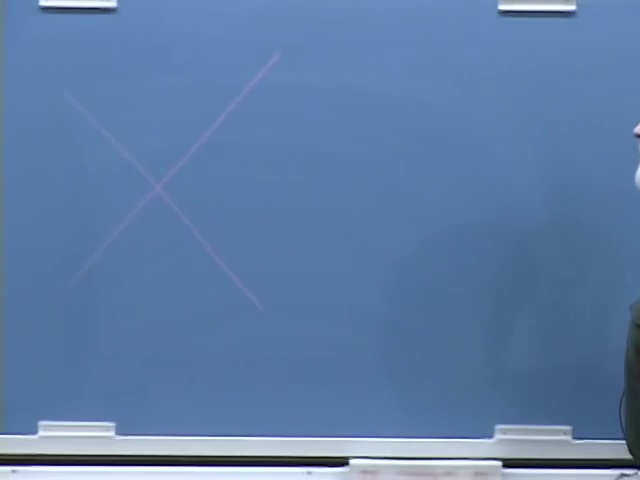
\includegraphics[width=0.68\textwidth]{lecture_09_figure_02.png}
\caption{Nhiệt độ Hawking \(T_H=1/(8\pi M)\) trong đơn vị tự nhiên.}
\lectureframe{00:08:12}
\end{figure}

Lỗ đen càng lớn thì càng lạnh. Bài giảng giải thích điều này bằng cách lần ngược một photon điển hình. Các photon nhiệt có năng lượng đặc trưng \(E_\gamma\sim T_H\). Một photon tới được vô cực với năng lượng cỡ \(M^{-1}\) đã có năng lượng cục bộ lớn hơn nhiều khi nó khởi đầu gần chân trời. Dịch đỏ giữa lớp gần chân trời và vô cực mạnh hơn đối với một lỗ lớn hơn, nên nhiệt độ ở vô cực thấp hơn.

\begin{classroomqa}
\audiencequestion{Nếu thời gian Schwarzschild bị đóng băng tại chân trời, có phải ta nên theo dõi photon ban đầu đã rơi vào và góp phần tạo nên lỗ đen không?\lecturetimestamp{00:04:19}}
\lecturerresponse{Đối với câu hỏi về nhiệt độ, hãy theo các photon phát ra theo hướng ra ngoài. Chúng bắt đầu với tần số cục bộ rất cao, mất năng lượng khi leo ra ngoài, và đến nơi như bức xạ Hawking. Số phận của photon ban đầu rơi vào là một câu hỏi thông tin riêng biệt.}
\end{classroomqa}

\section{Lớp Planck và chân trời kéo giãn}

Quan hệ cục bộ trong Phương trình~\eqref{eq:l09-local-temperature} có thể được tin cậy đến gần tới mức nào? Bài giảng lấy độ dài Planck làm khoảng cách ngắn nhất còn có ý nghĩa trong mô tả bán cổ điển. Điều này gợi ra một lớp mỏng, xấp xỉ một độ dài Planck bên ngoài chân trời toán học, chứa đầy các thăng giáng ở thang Planck. Nó liên tục phát xạ và hấp thụ.

Phần lớn các lượng tử phát ra không thoát được. Chỉ những lượng tử hướng vào một nón rất hẹp ra ngoài mới tránh rơi trở lại. Những lượng tử phóng đi ở các góc thông thường sẽ quay lại chân trời. Các kích thích đi ra và đi vào va chạm, tạo ra các cặp và những hạt khác; theo nghĩa này, mô tả đứng yên chứa một lớp vỏ mỏng gồm vật chất cực nóng.

\begin{figure}[htbp]
\centering
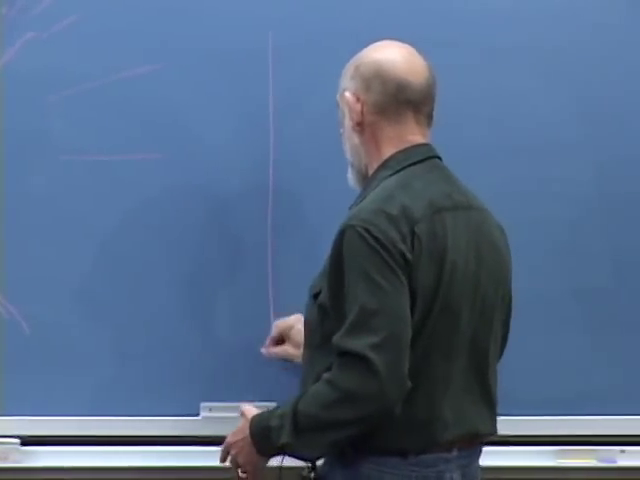
\includegraphics[width=0.74\textwidth]{lecture_09_figure_03.png}
\caption{Nón thoát hẹp của bức xạ gần chân trời. Phần lớn các lượng tử được phát cục bộ quay lại chân trời.}
\lectureframe{00:11:38}
\end{figure}

Có một bức tranh không-thời gian bổ sung. Xa chân trời, một thăng giáng ảo có thể được biểu diễn sơ đồ bằng một vòng kín ngắn: một kích thích hạt-phản hạt xuất hiện rồi biến mất trước khi nó có thể trở thành một trạng thái tiệm cận. Gần chân trời, một thăng giáng có thể bắc qua biên nhân quả. Đối với người quan sát bên ngoài, phần ở ngoài trông như một hạt do chân trời phát ra rồi về sau bị tái hấp thụ. Một phần rất nhỏ thoát ra và trở thành bức xạ Hawking.

\begin{classroomqa}
\audiencequestion{Trong giản đồ miền ngoài, một thăng giáng như vậy có kéo dài từ \(t=-\infty\) đến \(t=+\infty\) không?\lecturetimestamp{00:15:00}}
\lecturerresponse{Chân trời cổ điển chính xác dẫn đến mô tả trông có vẻ kỳ dị đó. Trên thực tế, ta thay nó bằng một chân trời kéo giãn, một siêu mặt kiểu thời gian cách ra ngoài chừng một độ dài Planck. Khi đó, sự phát xạ và tái hấp thụ xảy ra ở những thời gian miền ngoài hữu hạn.}
\end{classroomqa}

\begin{figure}[htbp]
\centering
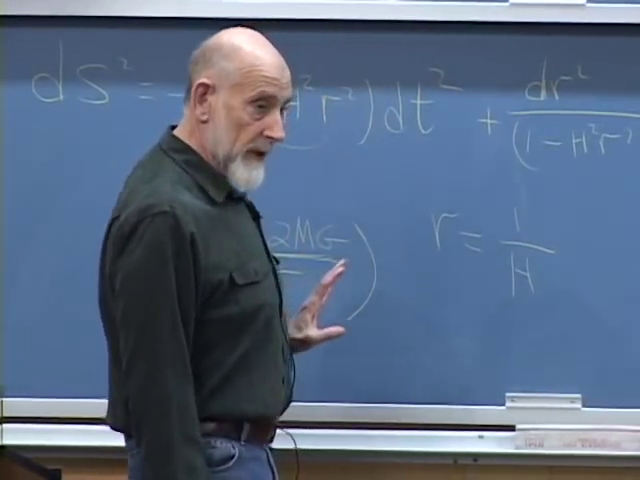
\includegraphics[width=0.72\textwidth]{lecture_09_figure_04.png}
\caption{Chân trời cổ điển và chân trời kéo giãn lân cận được dùng trong mô tả miền ngoài.}
\lectureframe{00:15:52}
\end{figure}

Chân trời kéo giãn không phải là một biên bất biến mới. Nó là một bề mặt hiệu dụng được đặt tại nơi hình học bán cổ điển không còn đáng tin cậy. Các thăng giáng lượng tử của vật chất và của chính hình học làm nhòe vị trí chính xác ở thang Planck. Cách dựng này gói sự bất định đó vào một bề mặt mà trên đó mô tả miền ngoài vẫn hữu hạn.

Không có gì trong lập luận cục bộ này phân biệt việc chân trời thuộc về một lỗ đen hay một vũ trụ đang gia tốc. Đó là chiếc cầu nối sang không gian de Sitter.

\section{Không gian de Sitter trong các tọa độ giãn nở}

Bài giảng chính thức bắt đầu bằng phép cắt phẳng theo không gian của không-thời gian de Sitter,
\begin{equation}
ds^2=-dt^2+e^{2Ht}d\mathbf{x}^2,
\qquad
d\mathbf{x}^2=dx^2+dy^2+dz^2.
\label{eq:l09-flat-slicing}
\end{equation}
Hằng số \(H\) là tốc độ giãn nở de Sitter. Thừa số xuất hiện dưới dạng \(e^{2Ht}\) vì metric đo bình phương khoảng cách; một khoảng tọa độ cố định có độ dài vật lý
\begin{equation}
D(t)=e^{Ht}\lvert\Delta\mathbf{x}\rvert.
\end{equation}

\begin{figure}[htbp]
\centering
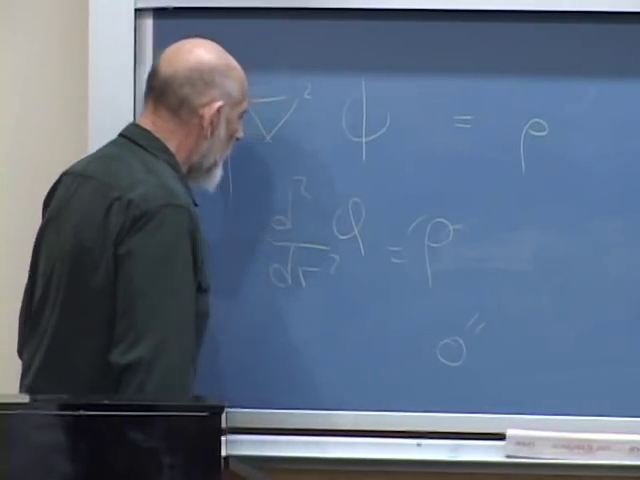
\includegraphics[width=0.78\textwidth]{lecture_09_figure_05.png}
\caption{Metric de Sitter giãn nở theo hàm mũ trong tọa độ phẳng.}
\lectureframe{00:18:50}
\end{figure}

Các tọa độ này làm sự giãn nở trở nên hiển nhiên nhưng đặt vô cực tương lai xa vô hạn lên phía trên trang. Để đưa nó lên bảng, ta đưa vào thời gian bảo giác
\begin{equation}
\eta=-\frac{1}{H}e^{-Ht},
\qquad
-\infty<\eta<0.
\label{eq:l09-conformal-time}
\end{equation}
Khi đó
\begin{equation}
dt=\frac{d\eta}{-H\eta},
\qquad
e^{Ht}=-\frac{1}{H\eta},
\end{equation}
và Phương trình~\eqref{eq:l09-flat-slicing} trở thành
\begin{equation}
ds^2=\frac{1}{H^2\eta^2}
\left(-d\eta^2+d\mathbf{x}^2\right).
\label{eq:l09-conformal-metric}
\end{equation}
Khi \(t\to+\infty\), \(\eta\to0^{-}\). Thời gian riêng vô hạn đã được nén thành đường ngang hữu hạn \(\eta=0\).

\editorialnote{Phép biến đổi thời gian được sửa nhiều lần trong lúc viết trên bảng. Phương trình~\eqref{eq:l09-conformal-time} là dạng nhất quán: thời gian vũ trụ sớm ánh xạ tới \(\eta\to-\infty\), còn vô cực tương lai ánh xạ tới \(\eta\to0^{-}\).}

\begin{figure}[htbp]
\centering
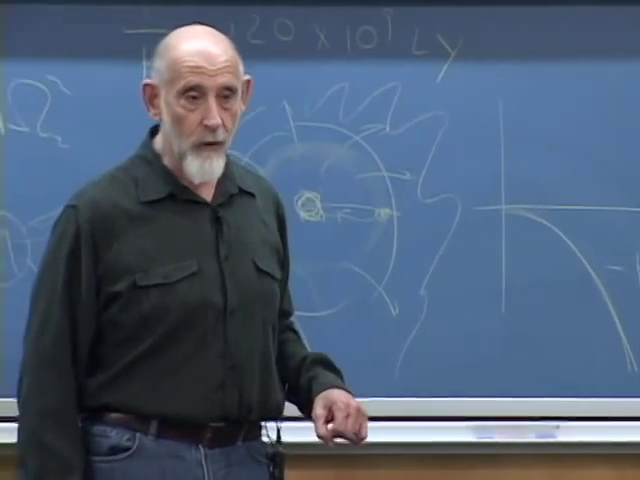
\includegraphics[width=0.82\textwidth]{lecture_09_figure_06.png}
\caption{Phép biến đổi sang thời gian bảo giác và metric phẳng bảo giác.}
\lectureframe{00:21:24}
\end{figure}

Thừa số bảo giác nhân vào cả hạng thời gian lẫn hạng không gian, nên nó không làm thay đổi các phương null. Đối với một tia sáng xuyên tâm,
\begin{equation}
ds^2=0
\quad\Longrightarrow\quad
-d\eta^2+dx^2=0
\quad\Longrightarrow\quad
\frac{dx}{d\eta}=\pm1.
\label{eq:l09-null-rays}
\end{equation}
Vì vậy ánh sáng truyền theo \(45^\circ\) trên giản đồ bảo giác. Đó là lý do phép đổi tọa độ này hữu ích: khả năng tiếp cận nhân quả trở nên nhìn thấy được.

\section{Miền nhân quả của một người quan sát}

Hãy hình dung một người quan sát có đường thế kéo dài trong thời gian riêng vô hạn. Trên giản đồ compact hóa, nó kết thúc tại một điểm trên \(\eta=0\). Mọi tín hiệu mà người quan sát ấy có thể nhận được đều nằm bên trong nón ánh sáng quá khứ của điểm cuối đó. Các sự kiện ở ngoài nón ấy sẽ không bao giờ có thể liên lạc với người quan sát, dù người đó chờ bao lâu đi nữa.

\begin{figure}[htbp]
\centering
\includegraphics[width=0.78\textwidth]{lecture_09_figure_07.png}
\caption{Nón ánh sáng quá khứ giới hạn của một người quan sát trong tọa độ de Sitter bảo giác.}
\lectureframe{00:24:38}
\end{figure}

Một người quan sát thứ hai có một nón khác. Hai miền có thể tiếp cận chồng lấn lên nhau, nhưng không miền nào là toàn bộ không-thời gian. Trong phần còn lại của lập luận, ta nhận quan điểm của người quan sát thứ nhất và gọi nón ánh sáng quá khứ đó là miền nhân quả của người quan sát.

Hình vẽ dường như cho thấy miền ấy co lại về phía tương lai, nhưng độ rộng tọa độ không phải là khoảng cách riêng. Trên một mặt cắt có \(\eta\) không đổi, bình phương khoảng cách vật lý giữa người quan sát tại \(x=0\) và chân trời tại \(x=\Delta x\) là
\begin{equation}
D^2=\frac{(\Delta x)^2}{H^2\eta^2}.
\label{eq:l09-horizon-distance-start}
\end{equation}
Chân trời là một đường null \(45^\circ\) kết thúc tại \(\eta=0\), do đó
\begin{equation}
\Delta x=\lvert\eta\rvert.
\end{equation}
Thay vào ta được
\begin{equation}
D_{\rm hor}^2=\frac{1}{H^2},
\qquad
D_{\rm hor}=\frac{1}{H}.
\label{eq:l09-horizon-radius}
\end{equation}
Độ tách tọa độ co lại, nhưng thừa số bảo giác tăng đúng bằng lượng bù trừ. Bán kính riêng của chân trời là hằng số.

\begin{figure}[htbp]
\centering
\includegraphics[width=0.80\textwidth]{lecture_09_figure_08.png}
\caption{Phép suy ra trên bảng chuyển khoảng tọa độ đang co lại thành khoảng cách riêng cố định \(H^{-1}\).}
\lectureframe{00:28:42}
\end{figure}

\section{Miền tĩnh}

Một bán kính chân trời cố định gợi ý một hệ tọa độ thích nghi với người quan sát ở tâm. Không suy ra phép biến đổi tọa độ, bài giảng viết kết quả:
\begin{equation}
ds^2=
-\left(1-H^2r^2\right)d\tau^2
+\frac{dr^2}{1-H^2r^2}
+r^2d\Omega_2^2.
\label{eq:l09-static-patch}
\end{equation}
Các hệ số phụ thuộc vào \(r\), chứ không phụ thuộc vào \(\tau\). Hệ tọa độ này bao phủ miền tĩnh của người quan sát,
\begin{equation}
0\le r<\frac{1}{H}.
\end{equation}

\begin{figure}[htbp]
\centering
\includegraphics[width=0.88\textwidth]{lecture_09_figure_09.png}
\caption{Metric miền tĩnh de Sitter và sự so sánh của nó với thừa số Schwarzschild.}
\lectureframe{00:34:22}
\end{figure}

Sự giống nhau với Schwarzschild hiện ra ngay lập tức:
\begin{equation}
f_{\rm dS}(r)=1-H^2r^2,
\qquad
f_{\rm Schw}(r)=1-\frac{2G_NM}{r}.
\end{equation}
Trong cả hai trường hợp, chân trời trong tọa độ tĩnh xuất hiện tại nơi \(f(r)=0\). Đối với de Sitter,
\begin{equation}
1-H^2r^2=0
\quad\Longrightarrow\quad
r_H=H^{-1}.
\end{equation}
Hệ tọa độ này kỳ dị tại đó, đúng như tọa độ Schwarzschild kỳ dị tại chân trời lỗ đen. Tuy vậy, các hình học toàn cục khác nhau theo một cách quan trọng. Người quan sát lỗ đen đứng ở bên ngoài và nhìn vào trong; người quan sát de Sitter đứng ở bên trong và nhìn ra ngoài.

\begin{classroomqa}
\audiencequestion{Làm sao hình học có thể tĩnh khi các hạt được buông tự do lại chuyển động xa nhau trong một vũ trụ giãn nở theo hàm mũ?\lecturetimestamp{00:36:06}}
\lecturerresponse{Tĩnh không có nghĩa là mọi hạt đều đứng yên. Nó có nghĩa là các hệ số của metric và kết quả của một thí nghiệm lặp lại không phụ thuộc vào thời điểm bắt đầu. Buông hai hạt bây giờ và chúng gia tốc tách xa nhau; lặp lại cùng thí nghiệm ấy về sau thì cùng chuyển động đó lại xảy ra.}
\end{classroomqa}

\begin{classroomqa}
\audiencequestion{Hai hạt đang tách xa nhau có thấy nhau bị dịch đỏ không?\lecturetimestamp{00:38:34}}
\lecturerresponse{Có. Sự tách xa ngày càng tăng của chúng tạo ra một dịch đỏ tương đối, dù metric thích nghi với người quan sát là độc lập theo thời gian.}
\end{classroomqa}

\section{Nhiệt độ nhìn từ bên trong}

Cấu trúc lân cận chân trời của không gian Schwarzschild và de Sitter là tương đương cục bộ. Vì vậy, chân trời de Sitter phát ra rồi tái hấp thụ các lượng tử nhiệt. Một photon hiếm hoi truyền vào trong tới người quan sát ở tâm, mất năng lượng khi leo ngược thế của miền tĩnh. Nhiệt độ Gibbons--Hawking đo tại tâm là
\begin{equation}
T_{\rm dS}=\frac{H}{2\pi}
\label{eq:l09-de-sitter-temperature}
\end{equation}
trong đơn vị tự nhiên. Một nhiệt kế đứng yên tại bán kính \(r\) đo được giá trị bị dịch đỏ theo Tolman
\begin{equation}
T_{\rm local}(r)=
\frac{T_{\rm dS}}{\sqrt{1-H^2r^2}},
\label{eq:l09-tolman}
\end{equation}
đại lượng này phân kỳ khi \(r\to H^{-1}\) và ở gần chân trời thì rút gọn về Phương trình~\eqref{eq:l09-local-temperature}.

\editorialnote{Bài giảng suy ra thang độ lớn từ khoảng cách tới chân trời và độ dịch đỏ thay vì viết tường minh các Phương trình~\eqref{eq:l09-de-sitter-temperature} và \eqref{eq:l09-tolman}. Ở đây nêu ra cách chuẩn hóa tiêu chuẩn của lập luận đó.}

Đối với gia tốc muộn quan sát được, bài giảng dùng ước lượng chu kỳ
\begin{equation}
H^{-1}\sim 20\times10^9\ {\rm light\ years}.
\label{eq:l09-lecture-horizon-estimate}
\end{equation}
Khi đó, một photon chân trời điển hình có bước sóng cỡ hàng tỉ năm ánh sáng. Đây không phải bức xạ nền vi sóng; nó lạnh hơn rất nhiều.

Thí nghiệm tưởng tượng mang tính thao tác là một cần câu ở quy mô vũ trụ học. Alice ở lại tại \(r=0\), gắn một nhiệt kế vào một sợi dây rất dài đồng thời truyền dữ liệu, rồi để lực đẩy vũ trụ đưa thiết bị ra ngoài. Cô dừng nó ngay trước chân trời, chờ tín hiệu quay về, và thấy một nhiệt độ cục bộ lớn. Nhiệt kế đặt cạnh cô ở tâm chỉ giá trị rất nhỏ \(H/(2\pi)\). Cùng một chân trời cho ra cả hai số đo vì chúng được thực hiện tại những thế hấp dẫn khác nhau.

\section{Vượt qua chân trời}

Mô tả cổ điển từ bên ngoài giống với câu chuyện hố đen quen thuộc. Bob ở tâm nhìn Alice lùi xa dần. Tín hiệu của cô bị dịch đỏ ngày càng mạnh và đến ngày càng chậm; cô dường như bị ép dẹt lên chân trời rồi cuối cùng mờ hẳn đi. Một người du hành đến sau, Jane, hiện ra như một lớp khác còn mỏng hơn trong một chồng trầm tích gần biên.

\begin{classroomqa}
\audiencequestion{Từ quan điểm của chúng ta, các vật thể có bao giờ đi qua chân trời vũ trụ không?\lecturetimestamp{00:45:30}}
\lecturerresponse{Không, trong mô tả cổ điển của người quan sát tĩnh. Tín hiệu của chúng bị dịch đỏ và mờ dần trong khi vị trí biểu kiến của chúng tiến sát chân trời. Tuy nhiên, trong mô tả rơi tự do của chính chúng, chúng đi qua mà không gặp một bề mặt kỳ dị cục bộ nào.}
\end{classroomqa}

\begin{classroomqa}
\audiencequestion{Chân trời chỉ nóng đối với các quan sát viên ở gần mà không băng qua nó thôi sao? Một người quan sát rơi vào không bị nấu chín chỉ vì đi qua nó, đúng không?\lecturetimestamp{00:48:27}}
\lecturerresponse{Alice đi qua trơn tru trong hệ quy chiếu riêng của cô. Nhiệt độ cực cao thuộc về mô tả đứng yên. Nếu Bob cứ khăng khăng phân giải Alice ngày càng sát chân trời, ông phải chiếu sáng cô bằng những bước sóng ngày càng ngắn. Khi đó, kính hiển vi Heisenberg trong nỗ lực ấy sẽ nạp vào đủ năng lượng để nấu chín chính thứ nó đang cố quan sát.}
\end{classroomqa}

Đây không phải là một mâu thuẫn giữa hai sự kiện cục bộ. Người quan sát đứng yên và người rơi vào dùng những phép đo khác nhau một cách căn bản. Tính bổ sung chân trời đặt câu hỏi làm thế nào cả hai mô tả đều có thể đúng mà không cho phép một người quan sát nào trực tiếp so sánh thông tin trùng lặp.

\section{Mô hình Newton của lực đẩy chân không}

Đến đây một sinh viên hỏi điều gì đóng vai trò thay cho giếng thế hấp dẫn của hố đen. Susskind trả lời bằng cách xây dựng một mô hình Newton. Gọi \(\phi\) là thế hấp dẫn, khi đó gia tốc của một hạt thử là
\begin{equation}
\mathbf{a}=-\boldsymbol{\nabla}\phi.
\end{equation}
Đối với vật chất thông thường không tương đối tính, phương trình Poisson là
\begin{equation}
\nabla^2\phi=4\pi G_N\rho.
\label{eq:l09-poisson}
\end{equation}

\begin{classroomqa}
\audiencequestion{Nếu các hiệu ứng của hố đen đến từ giếng thế hấp dẫn của nó, thì nguồn tương ứng trong không gian de Sitter là gì?\lecturetimestamp{00:49:36}}
\lecturerresponse{Chính năng lượng chân không cung cấp một nguồn hấp dẫn đồng nhất theo không gian. Trong mô tả Newton, nó tạo ra một thế bậc hai chứ không phải một giếng thế \(1/r\).}
\end{classroomqa}

\begin{figure}[htbp]
\centering
\includegraphics[width=0.78\textwidth]{lecture_09_figure_10.png}
\caption{Phương trình Poisson và dạng đạo hàm bậc hai theo bán kính mang tính sơ đồ trong bài giảng.}
\lectureframe{00:51:38}
\end{figure}

Trên bảng, người giảng lược bỏ hệ số chuẩn hóa, các hạng do độ đo cầu, áp suất, và lúc đầu thậm chí cả dấu tổng thể, khiến bài toán rút xuống còn
\begin{equation}
\frac{d^2\phi}{dr^2}\sim H^2.
\end{equation}
Suy luận cốt lõi là một nguồn hằng cho ra một hàm bậc hai. Với dấu cần có cho lực đẩy de Sitter,
\begin{equation}
\phi_{\rm dS}(r)=-\frac{1}{2}H^2r^2,
\qquad
a_r=-\frac{d\phi_{\rm dS}}{dr}=H^2r.
\label{eq:l09-de-sitter-potential}
\end{equation}
Gia tốc hướng ra ngoài và tăng tuyến tính theo khoảng cách. Giải \(\ddot r=H^2r\) thu được
\begin{equation}
r(\tau)=A e^{H\tau}+B e^{-H\tau},
\end{equation}
nên nhánh tăng tái tạo sự tách xa theo hàm mũ.

\begin{figure}[htbp]
\centering
\includegraphics[width=0.76\textwidth]{lecture_09_figure_11.png}
\caption{Phương trình nguồn đồng nhất và thế de Sitter bậc hai.}
\lectureframe{00:53:32}
\end{figure}

\editorialnote{Trong thuyết tương đối rộng, gia tốc trong gần đúng trường yếu của một lưu chất đồng nhất phụ thuộc vào \(\rho+3p\), chứ không chỉ vào \(\rho\). Năng lượng chân không có \(p=-\rho\), nên \(\rho+3p=-2\rho\) và gia tốc là đẩy ra. Phương trình~\eqref{eq:l09-de-sitter-potential} là kết quả de Sitter với chuẩn hóa đúng; phép tính trên bảng cố ý chỉ theo dõi phụ thuộc bậc hai và dấu.}

Đặt một khối lượng thông thường \(M\) tại tâm. Thế định tính khi đó trở thành
\begin{equation}
\phi(r)=-\frac{G_NM}{r}-\frac{1}{2}H^2r^2,
\label{eq:l09-combined-potential}
\end{equation}
và gia tốc theo bán kính là
\begin{equation}
a_r=-\frac{G_NM}{r^2}+H^2r.
\end{equation}
Khi \(r\) nhỏ, lực hút cục bộ thắng; khi \(r\) lớn, lực đẩy chân không thắng. Sự cân bằng của chúng xảy ra tại
\begin{equation}
r_\ast=\left(\frac{G_NM}{H^2}\right)^{1/3}.
\label{eq:l09-turnaround}
\end{equation}
Đây là phiên bản gọn gàng của cực đại thế trong bài giảng. Nó giải thích về mặt định tính vì sao các hệ bị liên kết hấp dẫn ở gần có thể vẫn ở cùng nhau trong khi những thiên hà đủ xa thì gia tốc rời xa nhau.

\begin{figure}[htbp]
\centering
\includegraphics[width=0.78\textwidth]{lecture_09_figure_12.png}
\caption{Lực hút thông thường \(1/r\) kết hợp với thế de Sitter bậc hai lật ngược.}
\lectureframe{00:58:20}
\end{figure}

\begin{classroomqa}
\audiencequestion{Các lực thông thường còn quan trọng không, hay lực đẩy chân không rốt cuộc sẽ xé toạc mọi hòn đảo vật chất?\lecturetimestamp{00:57:29}}
\lecturerresponse{Mọi lực đều phải được tính đến. Trên những thang đủ nhỏ, liên kết điện từ và hấp dẫn cục bộ chi phối. Lực đẩy chân không chỉ trở nên quan trọng trên những khoảng cách khổng lồ được đặt bởi \(H^{-1}\) và bởi thang cân bằng thích hợp với khối lượng liên kết.}
\end{classroomqa}

\section{Một nguồn, nhiều tên gọi}

Phần thảo luận giờ tạm dừng ở thuật ngữ. Năng lượng chân không, hằng số vũ trụ và năng lượng tối không phải là ba thành phần cộng gộp trong mô hình đang dùng. Chúng là ba cách mô tả cùng một nguồn \(w=-1\). Ta có thể nói tới một hạng hằng trong phương trình Einstein, một mật độ năng lượng chân không bất biến Lorentz, hoặc thành phần thúc đẩy gia tốc ở thời muộn.

\begin{classroomqa}
\audiencequestion{Nguồn Newton đồng nhất và năng lượng chân không lượng tử có cùng hiện diện như các hiệu ứng tách biệt không?\lecturetimestamp{00:59:14}}
\lecturerresponse{Không. Mật độ đồng nhất là mô hình Newton của cùng một nguồn đó. Năng lượng chân không, hằng số vũ trụ và, trong bài giảng này, năng lượng tối đều chỉ một thành phần vật lý.}
\end{classroomqa}

\begin{classroomqa}
\audiencequestion{Vậy cùng một hiện tượng có một mô tả cổ điển và một mô tả lượng tử phải không?\lecturetimestamp{01:00:32}}
\lecturerresponse{Nguồn gốc vi mô của nó có thể là cơ học lượng tử, cũng như một phần khối lượng của electron có nguồn gốc lượng tử. Một khi mật độ năng lượng hiệu dụng đã được biết, nó đi vào các phương trình hấp dẫn cổ điển như một nguồn thông thường. Chúng ta không biết nguồn gốc tối hậu của giá trị quan sát được.}
\end{classroomqa}

Trong đơn vị Planck, mật độ năng lượng chân không quan sát được là cực kỳ nhỏ,
\begin{equation}
\rho_\Lambda\sim10^{-123}\rho_{\rm Pl},
\label{eq:l09-planck-smallness}
\end{equation}
tùy theo quy ước dùng cho mật độ Planck. Con số nhỏ đó chính là bài toán hằng số vũ trụ. Đó cũng là lý do chân trời lại lớn đến vậy: trong bốn chiều,
\begin{equation}
H^2=\frac{8\pi G_N}{3}\rho_\Lambda,
\qquad
r_H=H^{-1}.
\end{equation}
Nếu \(H\) lớn hơn, chân trời sẽ nhỏ hơn, nhiệt độ de Sitter tại tâm sẽ cao hơn, và gia tốc đẩy \(H^2r\) sẽ mạnh hơn.

\begin{classroomqa}
\audiencequestion{Hằng số vũ trụ rất nhỏ có liên hệ với hằng số Planck và các dao động lượng tử không?\lecturetimestamp{01:03:27}}
\lecturerresponse{Phép so sánh gọn gàng nhất dùng các đơn vị Planck không thứ nguyên, trong đó \(G_N=\hbar=c=1\). Trong các đơn vị ấy, mật độ chân không thấp hơn mật độ Planck tự nhiên khoảng \(123\) bậc độ lớn. Giải thích sự phân cấp đó là một trong những câu đố trung tâm của vật lý cơ bản.}
\end{classroomqa}

\begin{classroomqa}
\audiencequestion{Năng lượng chân không có nhất thiết phải là một hằng số vũ trụ đúng nghĩa không đổi không? Thành phần gây gia tốc có thể giảm đi và cuối cùng về không không?\lecturetimestamp{01:04:52}}
\lecturerresponse{Đó là một khả năng thay thế hợp logic: một trường năng lượng tối động lực học có thể biến thiên theo thời gian. Bài giảng dùng trường hợp hằng vì những quan sát hiện có vào thời điểm đó ngày càng ủng hộ hành vi gần với một hằng số vũ trụ, chứ không phải vì mọi phương án thay thế đã được chứng minh là bất khả.}
\end{classroomqa}

\section{Thiên văn học trong tương lai xa}

Trong một vũ trụ tiệm cận de Sitter, các cấu trúc không bị liên kết hấp dẫn rốt cuộc sẽ đi qua chân trời của người quan sát. Phông vi sóng vũ trụ bị dịch đỏ xuống dưới ngưỡng phát hiện. Các thiên hà xa biến mất. Một nhà thiên văn còn lại có thể chỉ nhìn thấy một hòn đảo hấp dẫn địa phương đã sáp nhập nằm trong một vùng còn lại thì tối đen.

\begin{classroomqa}
\audiencequestion{Không có kính thiên văn, liệu có ai thậm chí nhận ra rằng các thiên hà xa đã biến mất không?\lecturetimestamp{01:06:17}}
\lecturerresponse{Có lẽ là không. Vấn đề nghiêm trọng hơn còn sâu hơn: ngay cả với các thiết bị tiên tiến, những người quan sát tương lai có thể thiếu các chỉ dấu xa và phông vi sóng mà từ đó ngày nay chúng ta suy ra sự giãn nở.}
\end{classroomqa}

Khi đó, bức tranh vũ trụ-đảo cũ có thể trở nên rất thuyết phục. Nghịch lý Olbers sẽ không buộc ta đi đến một kết luận khác, vì nó giả sử có một quần thể vô hạn, tĩnh và đồng đều của các nguồn sáng; người quan sát tương lai sẽ chỉ thấy các ngôi sao hữu hạn của hòn đảo địa phương. Năng lượng tối không liên tục tạo ra các thiên hà thay thế từ không gian trống rỗng.

Chân trời trong không gian de Sitter chính xác không co lại quanh thiên hà địa phương. Bán kính vật lý của nó vẫn là \(H^{-1}\), lớn hơn một thiên hà rất nhiều. Điều biến mất là vật chất không bị liên kết bị mang ra ngoài biên nhân quả cố định đó.

\begin{classroomqa}
\audiencequestion{Các ngôi sao bị bắn văng khỏi thiên hà có thể làm các vật thử để phát hiện hình học quy mô lớn không?\lecturetimestamp{01:11:25}}
\lecturerresponse{Trong một thời gian thì có. Các vật bị văng ra và các tín hiệu ánh sáng có đường cơ sở dài có thể thăm dò hình học. Nhưng hiệu ứng chỉ trở nên đáng kể trên những khoảng cách cỡ một phần đáng kể của một tỉ năm ánh sáng, nên thí nghiệm sẽ mất thời gian vũ trụ học.}
\end{classroomqa}

\begin{classroomqa}
\audiencequestion{Làm sao ta biết rằng một chân trời xa chưa che khuất phần lớn vũ trụ khỏi chúng ta?\lecturetimestamp{01:11:45}}
\lecturerresponse{Chúng ta đã nhìn thấy đủ nhiều thiên hà, độ dịch đỏ và bức xạ nền để đo sự giãn nở và phục dựng hình học quy mô lớn. Những người quan sát tương lai bị tước mất các chỉ dấu ấy sẽ đối diện một bài toán suy luận khó hơn nhiều.}
\end{classroomqa}

\begin{classroomqa}
\audiencequestion{Nếu chân trời nằm ngay bên ngoài Andromeda, sự hiện diện của nó có hiển nhiên không?\lecturetimestamp{01:12:19}}
\lecturerresponse{Có. Một chân trời nhỏ như vậy sẽ đòi hỏi \(H\) lớn hơn nhiều, và lực đẩy do đó sinh ra sẽ làm biến đổi mạnh chuyển động của Andromeda. Thay vào đó, giá trị đo được đặt chân trời tiệm cận ở một thang lớn hơn rất nhiều.}
\end{classroomqa}

\begin{classroomqa}
\audiencequestion{Những vụ nổ lớn mới có thể đang xảy ra bên ngoài chân trời của chúng ta không?\lecturetimestamp{01:13:25}}
\lecturerresponse{Các sự kiện bên ngoài chân trời là không thể nhìn thấy đối với chúng ta hoặc các hậu duệ của chúng ta. Một khả năng liên quan nhưng chính xác hơn, sự tạo mầm bong bóng trong lạm phát vĩnh cửu, sẽ được giới thiệu về sau trong bài giảng.}
\end{classroomqa}

Với tên lửa, đồng hồ và vài tỉ năm, những người quan sát tương lai có thể gửi các nhà thám hiểm đi qua một phần lớn của miền này và phục dựng metric của nó. Tuy nhiên, trên các thang thời gian phòng thí nghiệm hay văn minh thông thường, hiệu ứng ấy gần như ngoài tầm tiếp cận. Sự phân biệt này sửa lại khẳng định quá mạnh rằng sự giãn nở sẽ không thể được khám phá: về mặt thao tác nó rất xa tầm với, chứ không bị cấm về nguyên tắc.

\begin{classroomqa}
\audiencequestion{Liệu các nhà thám hiểm tương lai có thể xác định hình học sớm hơn rất nhiều so với việc chờ một lần hồi quy nhiệt hay không?\lecturetimestamp{01:21:40}}
\lecturerresponse{Chắc chắn là có. Một lần hồi quy không phải là phép đo được đề xuất. Các nhà thám hiểm trao đổi tín hiệu ánh sáng trên những đường cơ sở dài hàng tỷ năm ánh sáng có thể lập bản đồ vùng tĩnh trên một thang thời gian ngắn hơn rất nhiều, dù vẫn còn ở quy mô vũ trụ học.}
\end{classroomqa}

\begin{classroomqa}
\audiencequestion{Liệu dịch đỏ có xóa sạch mọi thông tin mà các nhà thám hiểm như vậy gửi về không?\lecturetimestamp{01:23:24}}
\lecturerresponse{Không, nếu họ thăm dò các thang nằm sâu bên trong chân trời. Một đường cơ sở cỡ một tỷ năm ánh sáng đã nhạy với sự giãn nở, trong khi chỉ tạo ra một dịch đỏ vừa phải. Thí nghiệm chủ yếu bị giới hạn bởi thời lượng khổng lồ của nó.}
\end{classroomqa}

\section{Entropy hữu hạn và sự hồi quy}

Vùng tĩnh không rỗng theo nghĩa nhiệt động học. Chân trời của nó có diện tích
\begin{equation}
A_H=4\pi H^{-2},
\end{equation}
nhiệt độ là \(T_{\rm dS}=H/(2\pi)\), và entropy
\begin{equation}
S_{\rm dS}=\frac{A_H}{4G_N}
=\frac{\pi}{G_NH^2}
\label{eq:l09-de-sitter-entropy}
\end{equation}
trong các đơn vị \(\hbar=c=k_B=1\). Entropy là hữu hạn. Vì thế, với sự dè dặt thích hợp, ta có thể hình dung vùng tĩnh như một khoang nhiệt có entropy hữu hạn, mà trong mô tả dừng thì các kích thích của nó tập trung gần chân trời.

Một hộp khí thông thường ở trạng thái cân bằng trông không có đặc trưng gì trên các thang thời gian ngắn, nhưng cơ học thống kê không cấm các thăng giáng. Nếu một trạng thái vĩ mô có độ hụt entropy \(\Delta S\) so với cân bằng, thì xác suất của nó xấp xỉ là
\begin{equation}
P\sim e^{-\Delta S}.
\label{eq:l09-fluctuation-probability}
\end{equation}
Thời gian chờ tương ứng tăng theo
\begin{equation}
t\sim t_0 e^{\Delta S}.
\end{equation}
Đối với một hệ hữu hạn, thời gian để quay lại một trạng thái gần tùy ý với một trạng thái trước đó là thời gian hồi quy Poincaré,
\begin{equation}
t_{\rm rec}\sim H^{-1}e^{S_{\rm dS}}.
\label{eq:l09-recurrence}
\end{equation}
Vì \(S_{\rm dS}\) đối với chân trời của chúng ta có bậc cỡ \(10^{120}\), bài giảng tóm tắt thang này là \(e^{10^{120}}\). Hệ số tiền nhân được đo bằng năm, thời gian Hubble hay các đơn vị vi mô đều không quan trọng so với hàm mũ kép.

\begin{figure}[htbp]
\centering
\includegraphics[width=0.76\textwidth]{lecture_09_figure_13.png}
\caption{Phần thảo luận về sự hồi quy, với thang thời gian chờ theo hàm mũ khổng lồ trên bảng.}
\lectureframe{01:16:24}
\end{figure}

Trước một lần hồi quy như thế, các thăng giáng nhỏ hơn phổ biến hơn rất nhiều. Các phân tử trong một căn phòng có thể đều tụ lại ở một góc; một xoáy phức tạp có thể thoáng hình thành; trong thứ bậc đùa vui của bài giảng, chuyển động nhiệt có thể lắp ghép nên một con voi. Độ hụt entropy cần thiết càng nhỏ, thăng giáng càng ít tốn kém.

\begin{classroomqa}
\audiencequestion{Liệu các hồi quy Poincaré có phải riêng là hệ quả của cơ học lượng tử không?\lecturetimestamp{01:25:44}}
\lecturerresponse{Không. Sự hồi quy và các thăng giáng hiếm đã xuất hiện ngay trong cơ học thống kê cổ điển. Việc áp dụng chúng vào không gian de Sitter sử dụng khuôn khổ vật lý hiện nay của chúng ta, khuôn khổ ấy có thể một ngày nào đó sẽ được sửa đổi, nhưng nhiệt động học và suy luận thống kê thuộc số những cấu trúc vững chắc nhất mà chúng ta biết.}
\end{classroomqa}

Bản thân ý nghĩa của xác suất có thể sẽ được hiểu sâu hơn trong một lý thuyết tương lai. Susskind không phủ nhận điều đó. Điểm ông muốn nêu hẹp hơn: từ bỏ cơ học thống kê chỉ vì những hệ quả ở thời gian dài của nó nghe kỳ lạ sẽ là vứt bỏ một trong những nguyên lý tổ chức của vật lý đã được kiểm nghiệm kỹ nhất.

\section{Não Boltzmann và các quan sát viên điển hình}

Giả sử một thăng giáng nhiệt tạo ra trọn vẹn một trạng thái giống Vụ Nổ Lớn. Điều đó đòi hỏi một sự giảm entropy khổng lồ. Một thăng giáng tạo ra một hệ hành tinh thì ít tốn kém hơn; một Trái Đất vốn đã ấm còn ít tốn kém hơn nữa. Nếu điều kiện duy nhất là có một quan sát viên, thì thăng giáng ít tốn kém nhất có thể chỉ tạo ra một bộ não đang hoạt động hoàn chỉnh kèm theo những ký ức bề ngoài có vẻ sẵn có. Một quan sát viên giả thuyết như vậy được gọi là một não Boltzmann.

Vấn đề không phải là liệu một thăng giáng kỳ quái nào đó có khả hữu về mặt lôgic hay không. Vấn đề là liệu một mô hình vũ trụ học có tiên đoán rằng hầu như mọi quan sát viên đều là một thăng giáng như thế hay không. Ta suy luận từ các quan sát của mình bằng cách giả sử rằng mình không dị thường đến mức khó tin. Một lý thuyết trong đó các quan sát viên thông thường với lịch sử vũ trụ mạch lạc bị các bộ não nhiệt cô lập áp đảo theo hàm mũ về số lượng sẽ phá hỏng suy luận ấy.

Vì vậy, bài toán não Boltzmann là tên gọi của một phép kiểm tra tính nhất quán định lượng. Người ta so sánh độ phong phú kỳ vọng của các quan sát viên thông thường với độ phong phú của các quan sát viên được sinh ra từ thăng giáng. Nếu loại sau chiếm ưu thế, thì hoặc chân không phải phân rã trước khi chúng tăng sinh, hoặc phải thay đổi độ đo, hoặc phải xem xét lại các giả định vũ trụ học.

Một câu hỏi trước đó về mối liên hệ tử ngoại--hồng ngoại được hoãn lại một cách minh thị. Lập luận về sự hồi quy không phụ thuộc vào việc giải quyết vấn đề tách biệt đó.

\section{Lạm phát vĩnh cửu và các vũ trụ bong bóng}

Tiếp theo, bài giảng giới thiệu, mà không cố gắng đưa ra một suy dẫn đầy đủ, một bài toán xác suất thứ hai. Một trạng thái chân không de Sitter giả bền có thể tạo mầm một bong bóng mà trong đó năng lượng chân không thấp hơn. Vách bong bóng giãn ra, và phần bên trong có thể phát triển thành một vũ trụ Friedmann--Robertson--Walker mở. Trong khi đó, miền đang lạm phát xung quanh tiếp tục giãn nở và tạo mầm thêm nhiều bong bóng.

\begin{figure}[htbp]
\centering
\includegraphics[width=0.74\textwidth]{lecture_09_figure_14.png}
\caption{Một bong bóng có năng lượng chân không thấp hơn được vẽ bên trong một nền de Sitter đang lạm phát.}
\lectureframe{01:29:38}
\end{figure}

Đặc trưng then chốt là sự tăng trưởng số lượng theo hàm mũ. Thể tích vật lý mới được tạo ra nhanh hơn tốc độ các bong bóng lấy đi nó, nên số miền bong bóng tăng lên không bị chặn. Các bong bóng khác nhau có thể lắng vào những trạng thái năng lượng thấp khác nhau và vì thế biểu lộ những vật lý hiệu dụng khác nhau.

Để phơi bày khó khăn thống kê, trước hết Susskind rời khỏi vũ trụ học và xét một dân số loài người tăng theo hàm mũ với nguồn lực hữu hạn nhưng chưa biết. Giả sử các quan sát viên là điển hình trong số tất cả những người từng sống. Nếu dân số tăng gấp đôi sau mỗi thế hệ rồi kết thúc, thì một nửa mọi người sống ở thế hệ cuối, ba phần tư sống ở hai thế hệ cuối, và bảy phần tám sống ở ba thế hệ cuối:
\begin{equation}
f_n=1-2^{-n}.
\label{eq:l09-last-generations}
\end{equation}
Khi đó, tính điển hình sẽ đặt chúng ta ở gần cuối một cách đáng ngại, mặc dù ta không biết gì về tổng nguồn lực. Điều này không được đưa ra như một dự đoán đáng tin cậy về sự tuyệt chủng của loài người. Nó là một lời cảnh báo rằng tăng trưởng theo hàm mũ khiến việc đếm bị chi phối bởi mốc cắt.

Ví dụ tung đồng xu phát biểu giả định điển hình thông thường một cách sáng sủa hơn. Nếu nhiều người làm thí nghiệm, mỗi người tung một đồng xu cân bằng \(N\) lần, thì đa số áp đảo sẽ thu được
\begin{equation}
n_H=\frac{N}{2}+O(\sqrt{N}).
\end{equation}
Một quan sát viên có kết quả cực đoan trước tiên nên nghi ngờ mô hình sai hoặc đồng xu có vấn đề, thay vì giả định vô bằng cớ rằng mình nằm trong một đuôi phân bố hiếm đến khó tin. Xác suất vũ trụ học dùng cùng trực giác về tính điển hình ấy, nhưng trong một quần thể vô hạn nó cần một cách đếm được xác định rõ.

\section{Biên của Escher và bài toán độ đo}

Phép loại suy hình học của Susskind là tác phẩm của M.\ C.\ Escher, \emph{Circle Limit IV}, một chiếc đĩa được lát kín bởi các thiên thần và ác quỷ trông nhỏ dần về phía biên. Trong hình học hyperbol được bức vẽ biểu diễn, các hình đó là tương đương; kích thước Euclid biểu kiến của chúng chỉ thay đổi vì phép chiếu.

\begin{figure}[htbp]
\centering
\includegraphics[width=0.76\textwidth]{lecture_09_figure_15.png}
\caption{Hình thay thế trên bảng cho các hình của Escher tăng sinh theo hàm mũ gần một biên tròn.}
\lectureframe{01:37:54}
\end{figure}

Hãy tưởng tượng Escher có thời gian, mực và sự kiên nhẫn đều hữu hạn. Gần mép, cuối cùng ông dừng lại, có lẽ để một số hình còn dang dở. Vì số lượng hình tăng theo hàm mũ theo bán kính hyperbol, một lớp ngoài hữu hạn chứa một phần cỡ đơn vị cố định của toàn bộ các hình đã vẽ. Xấp xỉ một nửa có thể nằm trong lớp cuối cùng, bất kể mốc cắt được dời ra xa đến đâu.

Bây giờ hãy hỏi tỉ số giữa thiên thần và ác quỷ. Trong mẫu hình vô hạn lý tưởng, tính đối xứng gợi ý sự bằng nhau một đối một. Tuy nhiên, trong bất kỳ phép đếm hữu hạn nào, một đường biên hơi khác đi cũng có thể bao hàm nhiều hơn hẳn các hình thuộc một loại. Vì phần lớn phép đếm nằm gần đường biên, một biến dạng nhỏ của đường biên ấy tạo ra một thay đổi cỡ đơn vị trong đáp án.

\begin{figure}[htbp]
\centering
\includegraphics[width=0.76\textwidth]{lecture_09_figure_16.png}
\caption{Biên cắt cụt chi phối phép đếm trong một mẫu hình tăng trưởng theo hàm mũ.}
\lectureframe{01:43:06}
\end{figure}

Sự mơ hồ tương tự cũng xuất hiện trong lạm phát vĩnh cửu. Hãy đếm các vũ trụ bong bóng xanh và hồng trước một mốc cắt theo thời gian nào đó, rồi đẩy mốc cắt ấy về muộn hơn. Cả hai phép đếm đều phân kỳ, và tỉ số của chúng có thể phụ thuộc nhạy vào việc \emph{thời gian} có nghĩa là gì và mặt cắt được vẽ như thế nào. Một độ đo xác suất là một quy tắc điều chỉnh quần thể vô hạn và rút ra các xác suất tương đối. Việc những quy tắc khả dĩ khác nhau không cho cùng một kết quả chính là bài toán độ đo.

\begin{classroomqa}
\audiencequestion{Có quan hệ nào giữa bài toán cắt cụt này và tái chuẩn hóa không?\lecturetimestamp{01:45:43}}
\lecturerresponse{Có một phép loại suy. Trong lý thuyết trường lượng tử, người ta đưa vào một mạng hoặc một cắt cụt tử ngoại, tinh chỉnh nó, và tìm những đại lượng không nhạy với các chi tiết ở rìa của bộ điều chuẩn. Các nhà vũ trụ học hy vọng có được một sự rút trích từ lạm phát vĩnh cửu cũng vững chắc như vậy, nhưng trong khuôn khổ đang được bàn ở đây vẫn chưa có một quy tắc có sức quyết định tương đương.}
\end{classroomqa}

Không nên đẩy phép loại suy này đi quá xa. Tái chuẩn hóa thành công khi một dòng chảy được kiểm soát xác định được các đại lượng quan sát được độc lập với bộ điều chuẩn. Bài toán độ đo chính là ở chỗ các câu hỏi bất biến tương tự và thủ tục lấy giới hạn vẫn còn chưa rõ. Nói rằng có thể ta đang đặt sai câu hỏi không phải là một lời giải cho đến khi câu hỏi đúng được cung cấp.

\begin{classroomqa}
\audiencequestion{Bức tranh bong bóng này có phải là cùng hiện tượng với lạm phát trong vũ trụ sơ khai của chúng ta không?\lecturetimestamp{01:48:19}}
\lecturerresponse{Nó có liên hệ rất chặt chẽ. Trong lạm phát vĩnh cửu, nền mẹ tiếp tục lạm phát trong khi phần bên trong cục bộ của các bong bóng trải qua tiến hóa vũ trụ học riêng của chúng. Vũ trụ quan sát được của chúng ta có thể nằm bên trong một miền như vậy.}
\end{classroomqa}

\section{Liệu có thể quan sát được các va chạm bong bóng không?}

Khi gặp nhau, hai bong bóng không đơn giản cộng năng lượng chân không của chúng lại. Một vách miền ngăn cách các miền có trạng thái chân không khác nhau, và hình học của vách quyết định mỗi phía có thể quan sát được gì. Tùy theo vị trí của va chạm so với nón ánh sáng quá khứ của chúng ta, dấu vết của nó có thể bị che khuất hoặc có thể nhìn thấy.

\begin{classroomqa}
\audiencequestion{Điều gì xảy ra khi hai bong bóng chân không va chạm?\lecturetimestamp{01:52:07}}
\lecturerresponse{Va chạm tạo ra một hình học vách miền mà hành vi của nó phụ thuộc vào hai chân không và vào sức căng của vách. Trong những hoàn cảnh nhân quả thuận lợi, nhiễu loạn có thể đi vào miền quan sát được của chúng ta và để lại một dấu hiệu bất đẳng hướng.}
\end{classroomqa}

Bài giảng bàn đến một vùng lạnh trong phông vi sóng vũ trụ như một ứng viên khả dĩ và chỉ ra phân cực quanh một đặc trưng hình tròn như một dấu hiệu phân biệt. Điều này được trình bày có chủ ý như một khả năng, chứ không phải một phát hiện. Một dấu hiệu va chạm đủ sức thuyết phục sẽ mang tính cách mạng vì nó sẽ cung cấp bằng chứng trực tiếp về các miền bong bóng lân cận và khiến bài toán độ đo trở nên cấp bách về mặt thực nghiệm.

\begin{figure}[htbp]
\centering
\includegraphics[width=0.70\textwidth]{lecture_09_figure_17.png}
\caption{Một đặc trưng tròn trên bầu trời và mẫu phân cực khả dĩ của nó trong phần thảo luận về va chạm bong bóng.}
\lectureframe{01:50:22}
\end{figure}

\editorialnote{Phần thảo luận về điểm lạnh ghi lại tình trạng quan sát và các đề xuất vào thời điểm của bài giảng. Bản thân một dị thường nhiệt độ không phải là bằng chứng của va chạm bong bóng; cần có một dấu hiệu chi tiết và tương quan.}

\begin{classroomqa}
\audiencequestion{Các bong bóng có phải là bốn chiều không, và phần bên trong của chúng có độ cong không gian nào?\lecturetimestamp{01:53:37}}
\lecturerresponse{Chúng là các miền không-thời gian, không phải các bong bóng xà phòng ba chiều tiến hóa trong một thời gian bên ngoài. Phần bên trong của chúng thường là các vũ trụ FRW mở với độ cong không gian âm. Một va chạm làm nhiễu loạn hình học đó nhưng không đơn giản biến độ cong âm thành độ cong dương.}
\end{classroomqa}

\section{Lý thuyết dây xác lập và không xác lập điều gì}

Phần thảo luận cuối cùng mở đầu bằng lời mời gán một xác suất cho việc lý thuyết dây là đúng. Susskind từ chối đưa ra con số ấy vì mệnh đề đó quá mơ hồ. Thay vào đó, ông tách ra hai khẳng định.

Thứ nhất, có một cấu trúc toán học bị ràng buộc rất chặt, kết hợp cơ học lượng tử và hấp dẫn. Nó đã đem lại những kết quả chính xác và các đồng nhất thức toán học sâu sắc, và tính nhất quán nội tại của nó đã đứng vững qua sự kiểm tra rộng rãi. Theo cách nói không chính thức của bài giảng, đó là \emph{String Theory} với chữ \(S\) viết hoa. Những phiên bản được hiểu rõ ràng nhất dựa rất nhiều vào siêu đối xứng.

Thứ hai, thế giới quan sát được không siêu đối xứng ở các năng lượng có thể tiếp cận. Việc kết nối các xây dựng siêu đối xứng chính xác với vũ trụ phi siêu đối xứng của chúng ta đòi hỏi sự phá vỡ siêu đối xứng và một khuôn khổ lớn hơn không được kiểm soát với cùng mức độ chính xác. Theo cách dùng từ của bài giảng, phần mở rộng được kỳ vọng đó là \emph{string theory} với chữ \(s\) viết thường.

\begin{classroomqa}
\audiencequestion{Có thể gán một xác suất cho khẳng định rằng lý thuyết dây là lý thuyết đúng của tự nhiên hay không?\lecturetimestamp{01:54:18}}
\lecturerresponse{Không thể làm vậy một cách có trách nhiệm nếu không chỉ rõ đang muốn nói đến khẳng định nào. Các cấu trúc toán học chính xác tồn tại và bao hàm hấp dẫn lượng tử, nhưng các mô hình siêu đối xứng được kiểm soát nghiêm ngặt không phải theo nghĩa đen là chính thế giới quan sát được của chúng ta. Việc một mở rộng lớn hơn có chứa thế giới của chúng ta hay không là vấn đề mà các nhà vật lý có thể có những thiên kiến dựa trên hiểu biết, chứ không phải một xác suất số được xác định rõ ràng.}
\end{classroomqa}

Phép tương tự ở đây là với cơ học vào thời kỳ trước khi bộ máy toán học đầy đủ trở nên sẵn có. Người ta có thể biết \(F=ma\) và lực nghịch đảo bình phương nhưng vẫn chỉ giải được các quỹ đạo tròn có đối xứng cao. Phần giải được ấy sẽ là thật, nhưng không phải toàn bộ lý thuyết. Tương tự, các xây dựng lý thuyết dây siêu đối xứng chính xác có thể là một miền đặc biệt, dễ xử lý một cách bất thường, của một cấu trúc lớn hơn.

\begin{figure}[htbp]
\centering
\includegraphics[width=0.60\textwidth]{lecture_09_figure_18.png}
\caption{Bức tranh lồng nhau của bài giảng: các xây dựng lý thuyết dây siêu đối xứng được kiểm soát nghiêm ngặt nằm bên trong một khuôn khổ lớn hơn mới chỉ ở mức phỏng đoán.}
\lectureframe{01:57:34}
\end{figure}

\begin{classroomqa}
\audiencequestion{Tại sao không đơn giản phá vỡ siêu đối xứng ngay trong lý thuyết chính xác?\lecturetimestamp{01:57:02}}
\lecturerresponse{Nhiều xây dựng gần đúng nghiên cứu sự phá vỡ siêu đối xứng, nhưng điều còn thiếu chính là bộ khung phi siêu đối xứng được kiểm soát hoàn toàn. Người ta có thể tính toán sau khi thực hiện các phép gần đúng chuẩn mà không phải lúc nào cũng biết đối tượng chính xác mà các phép gần đúng đó tiến tới.}
\end{classroomqa}

\begin{classroomqa}
\audiencequestion{Lý thuyết siêu đối xứng chính xác có loại trừ một mở rộng lớn hơn, ít đối xứng hơn, chứa thế giới của chúng ta hay không?\lecturetimestamp{02:00:33}}
\lecturerresponse{Không. Nó xác lập rằng thế giới quan sát được không được mô tả chỉ bởi riêng miền siêu đối xứng chính xác. Nó không chứng minh cũng không bác bỏ rằng miền này được nối với một lý thuyết lớn hơn chứa vật lý thực tế.}
\end{classroomqa}

\begin{classroomqa}
\audiencequestion{Các xây dựng lý thuyết dây có bao gồm sự phá vỡ đối xứng tương tự như sự phá vỡ đối xứng trong vật lý hạt hay không?\lecturetimestamp{02:01:21}}
\lecturerresponse{Có rất nhiều công trình về sự phá vỡ siêu đối xứng, và nhiều điều đã được biết về toán học siêu đối xứng. Điểm chưa được giải quyết là một công thức hóa chính xác, phi nhiễu loạn, kết hợp sự phá vỡ thực tế với lý thuyết đầy đủ thay vì chỉ với các phép gần đúng được kiểm soát.}
\end{classroomqa}

\begin{classroomqa}
\audiencequestion{Thuyết tương đối hẹp được giả định như một tiên đề trong lý thuyết dây, hay nó xuất hiện như một dự đoán?\lecturetimestamp{02:03:02}}
\lecturerresponse{Các quy tắc nền tảng là bất biến Lorentz, mặc dù một nền cụ thể chứa đầy vật chất có thể chọn ra một hệ quy chiếu nghỉ ưu tiên. Hấp dẫn còn không thể tránh khỏi hơn nữa: phổ dây chứa một kích thích spin hai không khối lượng với các tương tác của một graviton.}
\end{classroomqa}

\begin{classroomqa}
\audiencequestion{Lý thuyết dây có nhất quán với thuyết tương đối rộng và tính độc lập với nền hay không?\lecturetimestamp{02:04:11}}
\lecturerresponse{Động lực học hấp dẫn năng lượng thấp của nó nhất quán với thuyết tương đối rộng, và các nền cục bộ có thể được thay đổi một cách động lực học. Điểm tinh tế nằm ở các điều kiện biên tiệm cận: chúng gắn nhãn cho chính bài toán và nói chung không thể được thay đổi bằng một phép tác động cục bộ bên trong không-thời gian đó.}
\end{classroomqa}

Bài giảng khép lại bằng sự phân biệt đó giữa một cốt lõi toán học vững chắc và một sự ngoại suy vật lý còn dang dở. Đó không phải là một phán quyết rằng cốt lõi ấy vô dụng, cũng không phải là một khẳng định rằng phần ngoại suy ấy đã được xác lập. Đó là một phát biểu về chỗ mà tri thức chính xác chấm dứt.

\end{document}